% ******************************* PhD Thesis Template **************************
% Please have a look at the README.md file for info on how to use the template

% **************************** Formatting & Metadata ***************************

\documentclass[a4paper,12pt,times,numbered,print,chapter]{_Meta/thesis}
% See README.md for option details

% ******************************************************************************
% ****************************** Custom Margin *********************************

% Add `custommargin' in the document class options to use this section
% Set {innerside margin / outerside margin / topmargin / bottom margin}  and
% other page dimensions
\ifsetCustomMargin
  \RequirePackage[left=37mm,right=30mm,top=35mm,bottom=30mm]{geometry}
  \setFancyHdr % To apply fancy header after geometry package is loaded
\fi

% Add spaces between paragraphs
\setlength{\parskip}{0.5em}
% Ragged bottom avoids extra whitespaces between paragraphs
\raggedbottom
% To remove the excess top spacing for enumeration, list and description
%\usepackage{enumitem}
%\setlist[enumerate,itemize,description]{topsep=0em}

% *****************************************************************************
% ******************* Fonts (like different typewriter fonts etc.)*************

% Add `customfont' in the document class option to use this section

\ifsetCustomFont
  % Set your custom font here and use `customfont' in options. Leave empty to
  % load computer modern font (default LaTeX font).
  %\RequirePackage{helvet}

  % For use with XeLaTeX
  %  \setmainfont[
  %    Path              = ./libertine/opentype/,
  %    Extension         = .otf,
  %    UprightFont = LinLibertine_R,
  %    BoldFont = LinLibertine_RZ, % Linux Libertine O Regular Semibold
  %    ItalicFont = LinLibertine_RI,
  %    BoldItalicFont = LinLibertine_RZI, % Linux Libertine O Regular Semibold Italic
  %  ]
  %  {libertine}
  %  % load font from system font
  %  \newfontfamily\libertinesystemfont{Linux Libertine O}
\fi

% *****************************************************************************
% **************************** Custom Packages ********************************
% *****************************************************************************
% NB: Packages (without options) loaded in thesis class:
%  lscape, setspace, calc, ifthen, ifpdf, ifxetex, epstopdf, datetime,
%  everypage, textcomp, mathptmx, fourier, lmodern, amsmath, fontspec,
%  unicode-math, amsfonts, amssymb, url, breakurl, fancyhdr, makeidx,
% NB: Packages (with [options]) loaded in thesis class:
%  tocbibind[nottoc], appendix[title,titletoc], color[usenames, dvipsnames],
%  lineno[switch,pagewise,mathlines], textpos[absolute], graphicx[pdftex,demo],
%  biblatex[various options depending on other settings],
%  natbib[various options depending on other settings],
%  geometry[various options depending on other settings],
%  inputenc[utf8], fontenc[T1], microtype[final],
%  hyperref[unicode=true, hidelinks], nomencl[intoc],
%\usepackage{fancyvrb}
%\usepackage{framed}
\usepackage{subcaption}
\usepackage{wrapfig}
\usepackage{setspace}
\usepackage{todonotes}
\usepackage{tcolorbox}
\usepackage{threeparttable}
\usepackage{booktabs}
\usepackage{xstring}
\usepackage{mfirstuc}
\usepackage{xspace}
\usepackage{afterpage}
\usepackage{placeins}
\usepackage{array}
\usepackage[docdef=true,nonumberlist]{glossaries-extra}
\usepackage{textgreek}
%\usepackage{subfiles}
% ************************* Algorithms and Pseudocode **************************

%\usepackage{algpseudocode}


% ********************Captions and Hyperreferencing / URL **********************

% Captions: This makes captions of figures use a boldfaced small font.
%\RequirePackage[small,bf]{caption}

\RequirePackage[labelsep=colon,tableposition=top,labelfont=bf,font=small]{caption}
\renewcommand{\figurename}{Figure} %to support older versions of captions.sty


% *************************** Graphics and figures *****************************
\hyphenation{circRNA}
\hyphenation{circRNAs}

%\usepackage{rotating}

% Uncomment the following two lines to force Latex to place the figure.
% Use [H] when including graphics. Note 'H' instead of 'h'
%\usepackage{float}
%\restylefloat{figure}

% Subcaption package is also available in the sty folder you can use that by
% uncommenting the following line
% This is for people stuck with older versions of texlive
%\usepackage{sty/caption/subcaption}
\usepackage{subcaption}

% ********************************** Tables ************************************
\usepackage{booktabs} % For professional looking tables
\usepackage{multirow}

%\usepackage{multicol}
%\usepackage{longtable}
%\usepackage{tabularx}


% *********************************** SI Units *********************************
\usepackage{siunitx} % use this package module for SI units


% ******************************* Line Spacing *********************************

% Choose linespacing as appropriate. Default is one-half line spacing as per the
% University guidelines

% \doublespacing
% \onehalfspacing
% \singlespacing


% ************************ Formatting / Footnote *******************************
\usepackage{listings}

% Don't break enumeration (etc.) across pages in an ugly manner (default 10000)
%\clubpenalty=500
%\widowpenalty=500

%\usepackage[perpage]{footmisc} %Range of footnote options


% *****************************************************************************
% *************************** Bibliography  and References ********************

\usepackage{cleveref} %Referencing without need to explicitly state fig /table

% Add `custombib' in the document class option to use this section
\ifuseCustomBib
   %\RequirePackage[square, sort, numbers, authoryear]{natbib} % CustomBib

% If you would like to use biblatex for your reference management, as opposed to the default `natbibpackage` pass the option `custombib` in the document class. Comment out the previous line to make sure you don't load the natbib package. Uncomment the following lines and specify the location of references.bib file

\RequirePackage[backend=biber, citestyle=numeric-comp, style=nature, intitle=true, sorting=none, natbib=true, maxnames=3, minnames=1, url=false, giveninits=true, sortcites=true, date=year, doi=false,isbn=false]{biblatex}
\renewcommand{\intitlepunct}{\addspace\nopunct}
\bibliography{D_References/0_References}

\fi

% changes the default name `Bibliography` -> `References'
\renewcommand{\bibname}{References}


% ******************************************************************************
% ************************* User Defined Commands ******************************
% ******************************************************************************

% *********** To change the name of Table of Contents / LOF and LOT ************

%\renewcommand{\contentsname}{My Table of Contents}
%\renewcommand{\listfigurename}{My List of Figures}
%\renewcommand{\listtablename}{My List of Tables}

\usepackage{calc}
\makeatletter
\newcommand{\tocfill}{\cleaders\hbox{$\m@th \mkern\@dotsep mu . \mkern\@dotsep mu$}\hfill}
\makeatother
\newcommand{\abbrlabel}[1]{\makebox[8cm][l]{#1\ \tocfill}}
\newenvironment{abbreviations}{\begin{list}{}{\renewcommand{\makelabel}{\abbrlabel}%
        \setlength{\labelwidth}{8cm}\setlength{\leftmargin}{\labelwidth+\labelsep}%
                                              \setlength{\itemsep}{0pt}}}{\end{list}}

% ********************** TOC depth and numbering depth *************************

\setcounter{secnumdepth}{3}
\setcounter{tocdepth}{2}


% ******************************* Nomenclature *********************************

% To change the name of the Nomenclature section, uncomment the following line

%\renewcommand{\nomname}{Symbols}


% ********************************* Appendix ***********************************

% The default value of both \appendixtocname and \appendixpagename is `Appendices'. These names can all be changed via:

%\renewcommand{\appendixtocname}{List of appendices}
%\renewcommand{\appendixname}{Appndx}

% *********************** Configure Draft Mode **********************************

% Uncomment to disable figures in `draft'
%\setkeys{Gin}{draft=true}  % set draft to false to enable figures in `draft'

% These options are active only during the draft mode
% Default text is "Draft"
%\SetDraftText{DRAFT}

% Default Watermark location is top. Location (top/bottom)
%\SetDraftWMPosition{bottom}

% Draft Version - default is v1.0
%\SetDraftVersion{v1.1}

% Draft Text grayscale value (should be between 0-black and 1-white)
% Default value is 0.75
%\SetDraftGrayScale{0.8}


% ******************************** Todo Notes **********************************
%% Uncomment the following lines to have todonotes.

%\ifsetDraft
%	\usepackage[colorinlistoftodos]{todonotes}
%	\newcommand{\mynote}[1]{\todo[author=kks32,size=\small,inline,color=green!40]{#1}}
%\else
%	\newcommand{\mynote}[1]{}
%	\newcommand{\listoftodos}{}
%\fi

% Example todo: \mynote{Hey! I have a note}

%%%%%%%%%%%%%%%%%%%%%%%%%%%%%%%%%%%%%%%%%
%% UNIT COMMANDS FOR PROTOCOL TEMPLATE %%
%%      Will Bradshaw, March 2017      %%
%%%%%%%%%%%%%%%%%%%%%%%%%%%%%%%%%%%%%%%%%

% ******************************** Units **********************************

%% CUSTOM UNIT COMMAND %%
\newcommand{\cu}[2]{\SI[detect-weight]{#2}{#1}} % custom unit

%% TIME %%
\newcommand{\secs}{\cu{\second}} % Seconds
\newcommand{\mins}{\cu{\minute}} % Minutes
\newcommand{\hr}{\cu{\hour}} % Hours

%% VOLUME %%
\DeclareSIUnit\vols{vol} % volumes (relative to some reference)
\newcommand{\vol}{\cu{\vols}} % volumes
\newcommand{\ml}{\cu{\milli\litre}} % millilitres
\newcommand{\ul}{\cu{\micro\litre}} % microlitres
\newcommand{\lt}{\cu{\liter}} % litres

%% MASS %%
\let\ng\undefined
\newcommand{\ng}{\cu{\nano\gram}} % nanograms
\newcommand{\ug}{\cu{\micro\gram}} % micrograms
\newcommand{\mg}{\cu{\milli\gram}} % milligrams
\newcommand{\gr}{\cu{\gram}} % grams
\DeclareSIUnit\Unit{U} % enzyme units
\newcommand{\units}{\cu{\Unit}} % units of enzyme

%% CONCENTRATION %%
% Molar
\DeclareSIUnit\Molar{M} % Molar, = 1 mole per litre
\newcommand{\mol}{\cu{\Molar}} % molar
\newcommand{\mmol}{\cu{\milli\Molar}} % millimolar
\newcommand{\umol}{\cu{\micro\Molar}} % micromolar
\newcommand{\nmol}{\cu{\nano\Molar}} % nanomolar
% Mass per volume (e.g. for nucleic acids)
\newcommand{\ngul}{\cu{\nano\gram\per\micro\litre}} % ng/ul
\newcommand{\ngml}{\cu{\nano\gram\per\milli\litre}} % ng/ml
\newcommand{\ugml}{\cu{\micro\gram\per\milli\litre}} % ug/ml
\newcommand{\mgml}{\cu{\milli\gram\per\milli\litre}} % mg/ml
\newcommand{\gl}{\cu{\gram\per\liter}} % g/L
% Units per volume (for enzymes)
\newcommand{\unitsul}{\cu{\Unit\per\micro\litre}} % units/ul, for enzymes
% Percentages
\newcommand{\pc}{\cu{\percent}} % percent concentration (e.g. ethanol)
% Multiples
\DeclareSIUnit\X{\times} % x concentration, e.g. for buffers
\let\x\undefined
\newcommand{\x}{\cu{\X}}

%% TEMPERATURE %%
\newcommand{\degC}[1]{\SI[detect-weight]{#1}{\degreeCelsius}} % degrees celcius
\newcommand{\degrees}[1]{\SI[detect-weight]{#1}{\degree}}

%% PH %%
\DeclareSIUnit{\pH}{pH~}
\newcommand{\ph}[1]{\SI[detect-weight]{#1}[\pH]{}} % pH (as pre-unit)

%% CENTRIFUGE SPEED %%
\DeclareSIUnit{\G}{\mathit{g}} % x standard gravity
\DeclareSIUnit{\RPM}{rpm} % revolutions per minute
\newcommand{\g}[1]{\IfStrEq{#1}{top speed}{top speed}{\SI[detect-weight]{#1}{\G}}}
\newcommand{\rpm}{\cu{\RPM}}

%% BIOLOGICAL SEQUENCE LENGTH %%

\DeclareSIUnit{\B}{b} % Base (for kb etc)
\DeclareSIUnit{\BP}{bp} % Base pairs
\DeclareSIUnit{\NT}{nt} % Nucleotides
\newcommand{\bp}{\cu{\BP}}
\newcommand{\kb}{\cu{\kilo\B}}
\newcommand{\mb}{\cu{\mega\B}}
\newcommand{\nt}{\cu{\NT}}

%% LENGTH %%
\newcommand{\nm}{\cu{\nano\metre}}
\newcommand{\um}{\cu{\micro\metre}}
\newcommand{\mm}{\cu{\milli\metre}}


% ******************************** Autoref settings **********************************
%\renewcommand*{\sectionautorefname}{Section}
%\renewcommand*{\subsectionautorefname}{Section}
%\renewcommand*{\chapterautorefname}{Chapter}
%\newcommand*{\appendixautorefname}{Appendix}
%\newcommand*{\Appendixautorefname}{Appendix}

% ******************************** Misc. commands **********************************

\newcommand{\cm}[1]{C$_\mu$#1}
\newcommand{\cd}[1]{C$_\delta$#1}
\newcommand{\cz}[1]{C$_\zeta$#1}

\newcommand{\question}[1]{\subsection{#1}}
%\newcommand{\question}[1]{\textit{\Large #1}\\}
\newcommand{\q}[1]{\question{#1}}

\renewcommand\thesubfigure{\Alph{subfigure}}
\renewcommand\thesubtable{\Alph{subtable}}

\definecolor{codegreen}{rgb}{0,0.6,0}
\definecolor{codegray}{rgb}{0.5,0.5,0.5}
\definecolor{codepurple}{rgb}{0.58,0,0.82}
\definecolor{backcolour}{rgb}{0.95,0.95,0.92}

\lstset{
    backgroundcolor=\color{backcolour},   
    commentstyle=\color{codegreen},
	basicstyle=\ttfamily,
	columns=fixed,
	%frame=single,
    breaklines=true,
    breakatwhitespace=true,
    postbreak=\mbox{\textcolor{red}{$\hookrightarrow$}\space},
    language=bash,
    keepspaces=true,
    showstringspaces=false,
    aboveskip=-1.3em,
    belowskip=0.3em,
    upquote=true,
    }

% Quick formatting commands
\newcommand{\gene}[1]{\textit{#1}}
\newcommand{\igh}[1]{\gene{IGH{#1}}}

% Species names (with and without genus abbreviation)
\newcommand{\species}[2]{\textit{\capitalisewords{#1} #2}\xspace}
\newcommand{\nfu}{\species{Nothobranchius}{furzeri}}
\newcommand{\Nfu}{\species{N.}{furzeri}}
\newcommand{\xma}{\species{Xiphophorus}{maculatus}}
\newcommand{\Xma}{\species{X.}{maculatus}}


% Program/package names and code snippets
\newcommand{\program}[1]{#1}
%\newcommand{\program}[2][bash]{\lstinline[language=#1]{#2}} %[]
\newcommand{\snippet}[2][bash]{\lstinline[language=#1]{#2}} %[]

% IGH locus components
\let\dh\undefined
\newcommand{\vh}{VH\xspace}
\newcommand{\dh}{DH\xspace}
\newcommand{\jh}{JH\xspace}
\newcommand{\ch}{CH\xspace}

% File formats
%\newcommand{\fmt}[1]{\texttt{\MakeUppercase{#1}}}
\newcommand{\fmt}[1]{\MakeUppercase{#1}}
\newcommand{\format}[1]{\fmt{#1}}

% Sequence
\newcommand{\sequence}[1]{\texttt{\MakeUppercase{#1}}}

% Ig-Seq
\newcommand{\igseq}{IgSeq\xspace}
\newcommand{\Igseq}{immunoglobulin sequencing\xspace}
\newcommand{\IGSEQ}{Immunoglobulin sequencing\xspace}
\newcommand{\naive}{na\"{i}ve\xspace}
\newcommand{\Naive}{Na\"{i}ve\xspace}


%% Start of subappendices environment
%\AtBeginEnvironment{subappendices}{%
%\chapter*{Appendices}
%\addcontentsline{toc}{chapter}{Appendices}
%\counterwithin{figure}{section}
%\counterwithin{table}{section}
%}
%
%% End of subappendices environment
%\AtEndEnvironment{subappendices}{%
%\counterwithout{figure}{section}
%\counterwithout{table}{section}
%}

\makeatletter
\newcommand\notsotiny{\@setfontsize\notsotiny\@viipt\@viiipt}
\newcommand\evenlesstiny{\@setfontsize\notsotiny\@viiipt\@ixpt}
\makeatother

\newcommand{\subsubsubsection}[1]{\noindent\textit{#1}\noindent}

\newcommand{\etc}{\textit{et cetera}\xspace}

\renewcommand{\floatpagefraction}{.85}%
\renewcommand{\topfraction}{.85}%
\renewcommand{\bottomfraction}{.50}%

% Embed text values in thesis
\newcommand{\embed}[1]{\input{#1}\unskip}

\newcommand{\Caption}[2]{\caption[#1]{\textbf{#1:} #2}}


% Generate the glossary
\makeglossaries
 %Contains packages and user-defined commands and settings
%
%% ************************ Thesis Information & Meta-data **********************
%
% ************************ Thesis Information & Meta-data **********************
%% The title of the thesis
\title{Characterising antibody immunity and ageing in a short-lived teleost}

%% Subtitle (Optional)
%\subtitle{}
%\submissiontext

%% The full name of the author
\author{William John Bradshaw}

%% Department (eg. Department of Engineering, Maths, Physics)
\dept{aus Hastings} %! Really?

%% University and Crest
%\university{University of Cologne, Germany}
% Crest minimum should be 30mm.
\crest{
\includegraphics[width=0.5\textwidth]{_Meta/Logos/UoC_Crest}}

%% Use this crest, if you are using the college crest
%% Crest long miminum should be 65mm
%\crest{\includegraphics[width=0.45\textwidth]{University_Crest_Long}}

%% College shield [optional] 
% Crest minimum should be 30mm.
%\collegeshield{\includegraphics[width=0.2\textwidth]{CollegeShields/Kings}}


% Supervisor (optional)
% for multiple supervisors, append each supervisor with the \newline command
\supervisor{Dr. Dario Riccardo Valenzano}

%% Supervisor Role (optional) - Supervisor (default) or advisor
% \supervisorrole{\textbf{Supervisors: }}
%% if no title is desired:
% \supervisorrole{}

%% Supervisor line width: required to align supervisors
\supervisorlinewidth{\textwidth}

%% Advisor (optional)
%% for multiple advisors, append each advisor with the \newline command
%\advisor{Dr. A. Advisor\newline
%Dr. B. Advisor} %! Add TAC here?
     
%% Advisor Role (optional) - Advisor (default) or leave empty
% \advisorrole{Advisors: }
%% if no title is required
% \advisorrole{}

%% Advisor line width: required to align supervisors
%\advisorlinewidth{0.25\textwidth}


%% You can redefine the submission text:
% Default as per the University guidelines:
% ``This dissertation is submitted for the degree of''
%\renewcommand{\submissiontext}{change the default text here if needed}

%% Full title of the Degree
%\degreetitle{Doctor of Philosophy}

%% College affiliation (optional)
%\college{MPI for Biology of Ageing}

%% Submission date
% Default is set as {\monthname[\the\month]\space\the\year}
%\degreedate{September 2014} 

%%% Meta information
%\subject{LaTeX} \keywords{{LaTeX} {PhD Thesis} {Engineering} {University of
%Cambridge}}
 % Thesis title and author information, other metadata

% ***************************** Abstract Separate ******************************
% To printout only the titlepage and the abstract with the PhD title and the
% author name for submission to the Student Registry, use the `abstract' option in
% the document class.

\ifdefineAbstract
 \pagestyle{empty}
 \includeonly{A_Frontmatter/2_abstract-de,A_Frontmatter/3_abstract-en,C_Backmatter/declaration}
\fi

% ***************************** Chapter Mode ***********************************
% The chapter mode allows user to only print particular chapters with references
% Title, Contents, Frontmatter are disabled by default
% Useful option to review a particular chapter or to send it to supervisior.
% To use choose `chapter' option in the document class

\ifdefineChapter
 \includeonly{B_Chapters/3_Locus/Locus}
\fi

\begin{document}
\maketitle

%% ******************************** Front Matter ********************************
%% Dedication, abstracts, acknowledgements etc. - do this last.

%! Enable hiding frontmatter with class option
\frontmatter
% ******************************* Thesis Dedidcation ********************************

\begin{dedication} 
\doublespacing
\raggedleft
\textit{
\begin{LARGE}
Cre\'{e}r, c'est recombiner.\\
\end{LARGE}
-- Fran\c{c}ois Jacob \citep{hsu2015pathogen}}
\end{dedication}


% ************************** Thesis Abstract *****************************
{
\cleardoublepage
\setsinglecolumn
\chapter*{\centering \LARGE Kurzzusammenfassung}
\thispagestyle{empty}
Alternde Menschen zeigen einen stetigen R\"uckgang der adaptiven Immunfunktion, mit wichtigen Auswirkungen auf Gesundheit und Lebensdauer. Systemische Ver\"anderungen, die in der Struktur und Diversit\"at des Antik\"orperrepertoires mit dem Alter beobachtet werden, spielen eine wichtige Rolle in diesem immunoseneszenten Ph\"anotypen; die relativ lange Lebensdauer der meisten Wirbeltier-Modellorganismen macht eine gr\"undliche Untersuchung des alternden Immunrepertoires jedoch schwierig. Als nat\"urlich kurzlebiges Wirbeltier bietet der T\"urkise Prachtgrundk\"arpfling (\textit{Nothobranchius furzeri}) eine aufregende neue Gelegenheit, die Alterung des adaptiven Immunsystems im Allgemeinen und des Antik\"orperrepertoires im Besonderen zu untersuchen.

In dieser Arbeit habe ich eine Kombination aus bestehenden genomischen Assemblierungen und neu generierten Sequenzierungsdaten verwendet, um den Immunoglobulin-H-Ketten-Locus des T\"urkisen Prachtgrundk\"arpflings zusammenzusetzen, zu charakterisieren und mit Loci eng verwandter Arten zu vergleichen. Dies zeigt eine dynamische Locus-Entwicklung mit sich wiederholenden Duplizierungen und Verlusten des spezialisierten mukosalen Isotypen \textit{IGHZ}. Diese Ergebnisse unterst\"utzen eine hohe Evolutionsrate der Immunoglobulin-H-Ketten-Loci in den Teleostei und bilden eine solide Grundlage f\"ur die Forschung der vergleichenden evolution\"aren Immunologie in Zahnk\"arpflingen.

Nachdem ich die Immunoglobulin-H-Ketten-Locus-Sequenz in \textit{N. furzeri} charakterisiert hatte, nutzte ich sie, um Immunoglobulin-Sequenzierung gezielt f\"ur diese Spezies zu etablieren, welche eine quantitative Analyse des Antik\"orperrepertoires erm\"oglicht. Die Anwendung dieses Protokolls auf Ganzk\"orper-Fischproben ergab komplexe und individualisierte Antik\"orperrepertoires, die in der intraindividuellen Diversit\"at mit dem Alter rasch abnehmen und in der interindividuellen Variabilit\"at zunehmen. Dies zeigt, dass die Antik\"orperrepertoires von T\"urkisen Prachtgrundk\"arpflingen, entsprechend ihrer kurzen Lebensdauer schnelle Alterungsprozesse aufweisen. Dieser altersbedingte Diversit\"atsverlust war besonders stark in Darmproben - ein Ph\"anomen, das mit der konstanten ausgepr\"agten Antigenexposition an Schleimhautoberfl\"achen zusammenh\"angen kann und bisher nicht in einem Wirbeltier-Modell untersucht wurde. Zusammenfassend etablieren diese Ergebnisse den T\"urkisen Prachtgrundk\"arpfling als neuartiges Modell f\"ur die Erforschung von Immunoseneszenz in Wirbeltieren und bilden die Grundlage f\"ur zuk\"unftige Analysen von und Interventionsstudien an adaptiver Immunalterung.
}

% ************************** Thesis Abstract *****************************
% Use `abstract' as an option in the document class to print only the titlepage and the abstract.
\begin{abstract}
\textbf{Motivation:} %Circular RNAs are a special class of RNA forming a covalently closed loop through a process called back-splicing. Not much is known about the function of circRNAs. Only for a few well studied circRNAs, potential functions were shown, these include miRNA sponging, RNA binding protein (RBP) sponging, and regulation of their host gene's transcription. Circular RNAs can be identified in rRNA depleted RNA-Sequencing by detecting chimeric reads, which span a back-splice junction. A variety of circRNA detection tools exists but no tool is able to summarize and characterize the identified circRNAs. To perform accurate downstream analyses after circRNA detection, it is crucial to know the exact exon-intron structure of circRNAs. Recently, two tools were published, which identify alternative splicing within circRNAs. Here, I am presenting \texttt{FUCHS} and \texttt{FUCHS\textit{denovo}} to summarize circRNAs and reconstruct their exon-intron chain based on liner-splice signals of back-splice junction anchored reads.

\textbf{Methods:} %In this study, I compared three state of the art circRNA detection programs. Based on the best tool, I developed a Python-based pipeline called \texttt{FUCHS}: \textbf{FU}ll \textbf{CH}aracterization of circular RNA using RNA-\textbf{S}equencing. This pipeline summarizes circRNAs by their host genes, detects skipped exons, finds double-breakpoint fragments, generates circle-wise coverage profiles, and clusters these profiles. Running \texttt{FUCHS} on a mouse dataset indicated that annotated gene models are not always suited to describe the circRNA's exon-intron structure. Hence, I developed an additional module, \texttt{FUCHS\textit{denovo}}, to reconstruct the exon-intron structure based on linear-splice signals of back-splice junction anchored reads. To demonstrate how \texttt{FUCHS} and \texttt{FUCHS\textit{denovo}} perform, I ran both programs on a dataset of young and old murine hearts and young and old murine livers.

\textbf{Results:} %The comparison of three circRNA detection programs (\texttt{DCC}, \texttt{CIRI}, and \texttt{KNIFE}) indicated \texttt{DCC} as the fastest and most accurate circRNA detection program. Running \texttt{FUCHS} on four mouse samples revealed that heart circRNAs are less diverse but more abundant than liver circRNAs. Considering only annotated exons, the average length of circRNAs was 500 BP. Heart circRNAs were longer than liver circRNAs. From the obtained coverage profiles, I concluded that annotated gene models were not always matching the exon-intron structure of circRNAs. A \textit{de novo} reconstruction of the inner circle structure using \texttt{FUCHS\textit{denovo}} showed a gain of information of 15 \%. Furthermore, \texttt{FUCHS\textit{denovo}} identified alternative splicing in 8 - 10 \% of circRNAs. Performing a differential motif enrichment analysis of the flanking introns of circRNAs with alternative splicing over circRNAs without alternative splicing identified FOXO as a potential transcription factor driving alternative splicing in circRNAs. Binding motifs for CPEB1 and HOX were enriched in the flanking introns of circRNAs from host genes expressing many circRNAs over circRNAs from host genes expressing only one circRNA. To exemplify the value of the reconstructed circRNA models in downstream analyses, I performed a miRNA seed search and RBP motif search. Comparing the seed density of circRNAs and mRNAs showed that circRNAs were more densely populated with both, miRNA seeds and RBP motifs. This suggests that circRNAs could form an additional layer in the gene-regulatory network by competing with their host genes for miRNA or RBP binding.

\textbf{Availability:} %\url{https://github.com/dieterich-lab/FUCHS.git}

\end{abstract}

% ************************** Thesis Acknowledgements **************************

\begin{acknowledgements}      
A doctoral thesis in the life sciences might have a single author, but almost always has a great many direct and indirect contributors. Mine is no exception, and so I have a number of people to thank.

First, my sincere thanks to Dario Valenzano, who welcomed me into his research group in 2014 and has always been an enthusiastic, attentive and understanding supervisor. None of the work in this thesis would have been possible without him, and I would be a far poorer scientist without his mentorship and support.

Many past and present members of the Valenzano group have also actively contributed to my work. Patrick Smith performed the microbiota-transfer studies that were the inspiration for the project in the first place and supervised and mentored me through my first and most difficult year. Joanna Dodzian generously bred and provided the fish cohorts I used for the pilot and ageing experiments in \Cref{chap:igseq}. Rongfeng (Ray) Cui performed the genome assembly that was the foundation of the work in \Cref{chap:locus} and has provided a great deal of essential advice on both experimental procedures and computational analysis. My student supervisees, Linda Zirden, Lena Schlautmann, Pascha Hokama, and Davina Patel all made essential contributions to developing and testing the turquoise-killifish immunoglobulin-sequencing protocol; you were all great. Our tireless and wonderful technician, Aleksandra Placzek, has been an essential part of the \igseq project in the lab and performed several of the library preps; many of my favourite parts of this thesis would not have been possible without her. Most recently, Michael Poeschla has joined the repertoire-sequencing team and helped prepare the libraries for the final \igseq experiment in \Cref{chap:igseq}; I look forward to seeing where he takes the project in the future. I am sincerely grateful to all of them for their help, support, and enthusiasm. My thanks also to the rest of the Valenzano lab, particularly my fellow students David Willemsen, Jens Seidel, Miriam Popkes, Daniel Davila and Franziska Metge, for contributing their ideas and enthusiasm to my project and making the group such a pleasant and friendly place in which to work.

A number of external collaborators and other scholars whose also made vital contributions to this work. Kathrin Reichwald provided me with essential BAC clones and a substantial amount of important advice. John Beausang, Aleksandra Walczak, Thierry Mora and Susana Magadan helped me get started in the enormous and somewhat intimidating world of immune repertoire analysis, and Aleksandra in particular has repeatedly provided invaluable advice, introductions and insight. Jason Vander Heiden has tirelessly answered my many questions about the Immcantation pipeline and even made some changes to it on my request, while Quentin Marcou has been an invaluable help in getting to grips with his fantastic software \program{IGoR}. Many other researchers have responded to my pestering emails, given advice where I needed it, and generally been friendly, welcoming and generous with their time. I am grateful to you all.

The co-ordination team of the Cologne Graduate School of Ageing Research has consistently been amazing, and I have repeatedly been impressed at the depth of their dedication, sympathy and willingness to help us students with all our big and little problems. My sincere thanks to Daniela Morick, Doris Birker and Jenny Ostermann for all your help and support. Thanks also to Ruth Willmott, for her invaluable soft-skills and careers coaching; Jorge Boucas, Daniel Rosskopp and the rest of the bioinformatics core facility for their patient help and advice; and all the other people I have unaccountably failed to mention here whose assistence, friendship and support I have relied on throughout this lengthly process.

My family, of course, have been a constant source of love and support. Mum, Dad, Anna, thank you for everything. I love you. My love and thanks also to the rest of my family, especially Ron and Julie, for their enduring support and belief in me and my research. 

Finally, my deepest and sincerest thanks to Simon Woolf, without whom this entire long adventure would have been a great deal more difficult and a great deal less fun.
\end{acknowledgements}

%% *********************** Adding TOC and List of Figures ***********************
%%%
\tableofcontents
%%
\listoffigures
%%
\listoftables
%
\chapter{List of abbreviations}
\begin{abbreviations}
\item[bp] Base pair
\item[DNA] Deoxyribonucleic acid
\item[FDR] False discovery rate
\item[mRNA] Messenger RNA
\item[PCR] Polymerase chain reaction
\item[qPCR] Quantitative PCR
\item[RNA] Ribonucleic acid
\item[RNA-Seq] RNA-Sequencing
\item[T_m] Melting temperature
\item[t_{ext}] Extension time
\item[Ig-Seq] Immunoglobulin sequencing
\item[GSP] Gene-specific primer
\item[TSA] Template-switch adapter
\item[dNTP] Deoxyribonucleoside triphosphate
\end{abbreviations}

\section*{Units of measurement}

\begin{abbreviations}
\item[\ul{}] Microlitres
\end{abbreviations}


% TODO: Separate by section/type? E.g. units, ...
%\printnomenclature[space] space can be set as 2em between symbol and description
%\printnomenclature[3em]

%\printnomenclature
%
%% ******************************** Main Matter *********************************
\mainmatter\onehalfspacing
%
%!TEX root = ../thesis.tex
% TODO: Change this?

\chapter*{Investigating the adaptive immune system in the turquoise killifish: a dialogue}  
\onehalfspacing

% Chapter summary (should fit on title page)

%% Chapter 1 summary
% Should fit on chapter title page

\section*{Summary} % Fits one one page if 1.5-spaced, but not at double spacing


The turquoise killifish IgH locus resembles that of medaka, the most closely-related teleost species with a characterised \textit{IgH} locus, in several important respects, including an unusual IgM-TM splice pattern different from most teleosts and the absence of the teleost-specific antibody isotype IgZ/T. The shared absence of IgZ/T in these related species was particularly striking, as all previously-characterised teleost loci except medaka and grasscarp have been found to possess this isotype. Given their relatedness, it was hypothesised that \dots

%\pagebreak

\section{First questions}

\q{Let's start with the basics. What is your thesis about?}

I think you can divide my thesis work into three main parts. First, the characterisation of the killifish immunoglobulin heavy chain locus. Second, the establishment of immunoglobulin sequencing in the killifish. And third, the use of those first two things to investigate how the killifish repertoire changes with age and (hopefully) with microbiota transfer. 

\q{Step back a second. Why did you do this? What was the point?}

The adaptive immune system is an extremely important part of vertebrate biology, and one whose performance declines dramatically with age. We wanted to find out more about why and how this happens and how it interacts with the ageing of other important systems we investigate in our lab, like the gut microbiota. In our lab we use the turquoise killifish as a model for vertebrate ageing -- it's the shortest lived vertebrate that lives in captivity and is therefore very convenient for investigating ageing, especially of vertebrate-specific systems that can't be studied in worms or flies. However, before this project very little immunological work had been done in this system. So it seemed to us that establishing the TK as a model organism for immunology, and especially immunosenescence, could be very valuable.

\q{That explains the killifish -- we'll talk more about the details of the model later. But why does that lead to the specific research questions you mentioned?}

The adaptive immune system is an example of a vertebrate-specific system whose ageing can't be studied in short-lived invertebrate systems. Both B- and T-cell-based adaptive immunity are very important and sophisticated, and both seem to undergo complex and profound ageing in humans. Both also seem to have important interactions with the microbiome. B-cells are unique in their ability to target unprocessed antigens, the diversity of the antigens they can respond to, and the ability of their antigen-receptor proteins -- antibodies -- to bind antigen and act in the immune system independently of the cell that produced them, through the production of secreted antibodies that bind antigen in serum or mucosal environments. All of this makes antibody immunity extremely important for host-microbiota interactions, as well as playing a key role in the adaptive immune system more generally. In the end, though, I could come up with equally good arguments for focusing on T-cells, and I'm not sure how much microbiota work there will be in this thesis at all, so the final answer is: I had to pick one or the other, and I picked B-cells.

\q{We'll talk more about B-cell immunity and repertoires later -- you've discussed them substantially elsewhere so we don't really need to cover them now. Let's take it as read that we agree immune-repertoire sequencing is interesting and relevant, and that establishing it in the TK is a worthwhile goal. The question remains: why did you spend so much time and energy characterising the IgH locus in killifish?}

The structure of the IgH locus provides the fundamental substrate of antibody diversification in a species, defining the space of possible sequences arising from the VDJ recombination process, the functional antibody classes available via the constant-region exons, and the possible splicing behaviour of those exons. The IgH CDR3 junctional region is by far the most diverse part of an antibody complex, and displays far more sequence diversity than any part of the immunoglobulin light chain. In order to understand anything about IgH diversity in the killifish, it is necessary to have a good baseline of possible variable segments that can be selected from; many tools depend on this for their performance. The structure and sequence of the constant regions is also important to define primer sequences for immunoglobulin sequencing, as well as interesting in its own right as being fundamental to antibody functionality in the species.

There is also an important comparative and evolutionary aspect to the IgH locus structure that isn't directly relevant to immunoglobulin sequencing and may or may not be relevant for ageing, but is interesting in its own right. Only a few (on the order of 10) teleost IgH loci have been previously characterised, but that is enough to reveal a very high level of sequence, structural and splicing diversity. Some teleost loci are highly simple, while others are highly complex and repetitive. There is also variation in which isotypes (antibody classes) are present among teleosts, with potentially important implications for their immune function. On a high level, this isn't very surprising given the vast diversity of teleost fish -- it's like saying that the immune systems of mammals, birds and frogs are all importantly different. However, we know very little about the patterns or rate of locus structure evolution.

When so few loci have been characterised from such a vast group of animals, adding one more from a new clade is useful enough in itself. However, I also had access to high-quality genome assemblies from a number of related killifish and non-killifish species, and was able to characterise the IgH loci in these species as well (though not to the same quality or completeness as for TK). This enabled me to compare the loci of a group of related species, which isn't something that had ever been done previously. And it let to some surprising findings.

So characterising the IgH locus was an important step on the road to establishing TK as an immunological model system and setting up IgSeq in that species, as well as raising interesting research questions in its own right.

\q{There's a lot to unpack there, and a lot of background we're going to need to talk about at some point. One more question before we move on to the details of the locus work: even if you didn't want to look at the TCR, why didn't you apply this to the light chains as well?}

Two reasons: time and relevance. I'm pretty sure I have everything I'd need to characterise the light chain loci in TK, and possibly in the other species too, but I doubt I'll have time to do it in time for my thesis submission. It's also much less relevant and important than the heavy chain, since light chain sequences aren't included in my IgSeq pipeline or data, and the light chain is much less important for antigen specificity than the heavy chain. It's still important, though, and someone will need to do it eventually, especially if IgSeq in the killifish progresses to more sophisticated methods that obtain heavy-light pairing information. 

There are also highly likely to be multiple light-chain loci in each genome, and if they are like other teleosts the structure will be much more of a cluster configuration than the semi-translocon configuration seen in the IgH loci. So in addition to being a lower priority, it's also likely to be a very slow and fiddly task, which doesn't fit neatly into the thesis. So it just wasn't a priority task compared to everything else I needed to do. In an ideal world, I'd have done it.

\q{Fair enough, though you probably want to smoothen that up for the actual thesis. Let's move on to the details of the locus characterisation and results, okay?}

Okay, sure.

\section{The turquoise killifish IgH locus}

\q{So how did you go about characterising the locus? We don't need the extreme details here, that can wait for the methods section, but we'd like to know the principles of how you did it.}

The characterisation of the TK IgH locus  involved the collection and interrelation of three sets of data. The first was information about V, D, J and constant-region sequences from other species whose loci had already been characterised, and for which reasonably informative public data was available. I tried a range of different species but eventually settled on zebrafish, stickleback as being most amenable to this task; all three provided enough sequence data and other information to infer most of the information I needed, which was not the case for many other published loci; conveniently, medaka and stickleback are also relatively closely related to TK, especially medaka. Even so, extracting good databases of locus segment sequences was not a quick or easy task; but you said not to get too into the nitty-gritty here.

\q{Yes, save that for later. So you obtained sequence databases from other species; why is this useful?}

Two reasons. Firstly, it allowed me to identify potential locus scaffolds from the killifish genome on the basis of alignments to those reference DBs. Secondly, once I had a locus sequence, they formed the basis of my pipeline for finding gene segments in the killifish locus.

\q{Okay, makes sense. By the way, you said medaka and stickleback are closely related to TK; is zebrafish not?}

Within the teleosts, zebrafish is very distantly related to any of medaka, stickleback and killifish. There are two major radiations within the teleosts, and zebrafish falls into one while the others fall into the other. I don't know the divergence time off the top of my head, but it's large.

\q{We'll want to see a tree for that.}

I'll make one. I'll need it for the evolutionary part of the locus chapter anyway.

\q{Alright. Moving on. What where the other sources of data you used?}

The second, of course, was the killifish genome. Several versions of the TK genome have been promulgated, and I used all of them at different points in my thesis, but the final locus is based on the best and most recent version, which doesn't currently have an official release designation, but will be published soon. I was fortunate in that the IgH locus in this version is relatively intact; in previous versions it was extremely fragmented, as is usually the case for antigen-receptor loci in \textit{de novo} assembled genomes. Though that's probably jumping ahead a bit.

Given a good-quality genome assembly and sets of reference sequences, I could align the latter to the former to identify genome scaffolds I thought might contain parts of the locus. This process identified one chromosome (chr6) which appeared to contain a relatively intact locus structure, plus several promising smaller scaffolds.

\q{Let's start with the chromosome. What does it mean to say that it appeared to contain a relatively intact locus?}

It contained extended V-, J- and C-regions, in the expected order (V-D-J-CM-CD) and with a common orientation (on the sense strand). The V- and J-region each consisted of multiple aligned segments. The C-region contained complete sets of \cm{} and \cd{} exons, in order. It also contained a single VH in antisense some distance downstream of this group of sequences, suggesting a potential second sublocus in antisense that was missing from the chromosome assembly. Multiple complete or semi-complete subloci in tandem is a common feature of teleost IgH loci, and the final sublocus of the medaka locus also appears to be in antisense, so this would make sense as a proposed locus structure.

\q{What would constitute ``complete sets of \cm{} and \cd{} exons"?}

Teleost IgM nearly always consists of six exons, four constant exons (\cm{1} to \cm{4}) and two transmembrane exons. Teleost IgD is more variable but typically consists of seven or more \cd{} exons and two TM exons. The reference alignments to chromosome 6 matched this structure. However, I didn't go into more detail about that at this stage; this was just to identify scaffolds, the detailed locus annotation came later.

\q{You mentioned extended V- and J-regions. What about the D-segments?}

D-segments are very short -- typically only 10bp or so. Not long enough to identify reliably using cross-species sequence alignment.

\q{Speaking of alignment, how did you map the reference species segments to the TK genome?}

I used BLAST. BLASTN for aligning reference nucleotide sequences, TBLASTN for aligning reference protein sequences. Then I filtered out low-scoring alignments and collapsed overlapping alignments together into a single annotation per sequence region. I can go into more detail; the complete process was quite involved.

\q{No, that's alright. Do you think that was a defensible course of action?}

BLAST is still the standard heuristic alignment tool used for these sorts of processes. Later on in the pipeline I used a mixture of BLAST and other aligners depending on the situation, but I think for this purpose it's more than adequate. I always checked the exact segment boundaries manually anyway, so I didn't rely too much on the exact alignment co-ordinates.

By the way, do you want me to explain how BLAST works?

\q{Let's save that for later. What did you mean when you said several other scaffolds were ``promising"?}

In order for genome scaffolds to be included for downstream consideration by the pipeline I wrote, they needed to either contain alignments to multiple different types of sequence (for example, different constant exons, or both V- and J-alignments) or have alignments to one sequence type covering more than a threshold proportion (1\%) of the scaffold length. This excluded most scaffolds containing one or two promising V-like segments isolated within a long stretch of non-IgH sequence, while keeping those scaffolds most likely to form part of the locus.

\q{How many scaffolds were ``promising" by this definition?}

Six:

\begin{threeparttable}
\begin{tabular}{ccccccc}\toprule
Scaffold & Total length (kb) & V & J & \cm{} & \cd{} & \cz{} & Included in locus?\\
chr6 & 6195.6 & 15 & 7 & 5 & 11 & 0 & Yes\\
scf10901 & 1.4 & 0 & 0 & 0 & 3 & 0 & Yes\\
scf21863 & 13.5 & 1 & 0 & 0 & 0 & 0 & No\\
scf35954 & 16.3 & 3 & 0 & 0 & 0 & 0 & No\\
scf36277 & 18.9 & 2 & 1 & 0 & 0 & 0 & No\\
scf37083 & 17.7 & 1 & 0 & 0 & 0 & 0 & No\\
scf9157 & 7.2 & 0 & 7 & 4 & 0 & 0 & Yes\\
\end{tabular}
\caption{Summary of genome scaffolds containing putative \textit{IgH} locus fragments}
\end{threeparttable}

\q{Impressive that you can speak in tables like that. It looks like you still have a few scaffolds with one or two V's and nothing else.}

Yes, and I excluded these \textit{a priori} for non-TK species. But in this case it wasn't an issue.

\q{Why not?}

Because I had other sources of information I could use to produce a contiguous locus sequence, and decide whether or not a given scaffold fell within the locus or not.

\q{What information was that?}

The third source of data I mentioned at the start of this section: bacterial artificial chromosome inserts covering parts of the killifish locus.

\q{Tell us about those}

Bacterial artificial chromosomes are long-insert \textit{E. coli} plasmids commonly used to hold extended stretches of eukaryotic DNA during genome assembly projects. In this context, they provide both long-range physical mapping information and the option to sequence specific contiguous stretches of the genome at elevated coverage. Since you know that the BAC insert represents a contiguous stretch of genomic DNA, assembling the insert sequence provides a high-confidence assembly of that part of the genome -- which you can then align to other BAC inserts to obtain a longer contiguous sequence.

When I started this project, there was no good genome assembly of the IgH locus available, so we adopted an alternative approach of identifying BACs containing part of the locus, sequencing them and characterising locus sequence from those. That gave us part of the locus; once the new genome was available, it proved sufficient to generate a complete locus assembly when combined with the scaffolds identified above.

\q{How did you identify candidate BACs?}

That's a complicated question. We identified the first group of BACs based on the small fragments of the locus available on the existing genome assemblies, combined with synteny. Those inserts gave us part of the locus, which we used to identify new BACs we thought would give us the rest. Those gave us more; the new genome assembly gave us the rest.

\q{Wait, wait. That's not an adequate answer. What do you mean, "based on small fragments of the locus"? What do you mean, "combined with synteny"? How did you use the first set of BACs to identify the second.}

As part of one of the killifish genome assembly projects, a BAC library of the killifish genome was generated, and the ends of a subset of those BACs were sequenced. That meant that it was possible to identify BACs whose ends aligned within or close to a particular sequence region, scaffold or locus. In the first case, an external collaborator identified BACs whose ends fell in scaffolds that either contained part of the locus, or were suspected on the basis of synteny to be immediately up- or downstream of it. In the second case, the BAC end alignment database had been made available, and it was possible for me to manually identify BACs whose inserts, based on their end alignments, should contain parts of the locus we were missing. For example, many BACs had ends aligning upstream of the 5' part of the locus, pointing into a large gap in the then-available genome assembly. Sequencing those BACs enabled me to extend that 5' part of the locus further, and identify more segments.

\q{You still need to develop this a lot more. How did you get the sequences you used for the first set of BACs? How did you identify BACs "on the basis of synteny"?}

I know I need to develop this more, but I don't have that information to hand. Let me get back to you about this.

\q{Mhm. This is pretty fundamental. How can we trust your conclusions if we don't know where the sequences came from?}

I know, I need to expand on this. But I'd rather focus on downstream areas right now.

\q{Okay, so you got the BACs somehow. How did you get the sequences?}

I isolated the BACs using alkaline lysis of the appropriate \textit{E. coli} clones; more details to follow. Then I sequenced them in collaboration with the Cologne Centre for Genomics on the Illumina MiSeq platform, 2x300bp. I should probably put a table of read numbers here.

Anyway, after getting the reads back, I trimmed them based on quality with Trimmomatic, filtered out reads aligning to \textit{E. coli} or \textit{H. sapiens} with Bowtie2, and assembled them with SPAdes. The resulting assemblies were scaffolded using SSPACE, and further assembly was performed by (a) aligning BAC scaffolds to each other and existing genome scaffolds, and (b) manual assembly using PCR and Sanger sequencing. In the end, I achieved complete or almost complete insert assemblies for a number of BACs I don't have immediately to hand. I then aligned these inserts together with BLAST to produce two larger sublocus sequences, corresponding to the 5' and 3' regions of the IgH locus, respectively. These were aligned to and integrated with the genome scaffolds identified earlier to produce a continuous locus sequence. 

\p{How did you integrate the genome scaffolds with the BAC-derived locus regions?}

I started by aligning the scaffolds to the BAC-derived regions and identifying extended regions of agreement, with a particular focus on the relationship between the chr6 locus region and the BAC regions. Several low-confidence scaffold candidates were not found to align with either the chr6 locus sequence or the BAC-derived locus regions, and were discarded; two non-chromosome candidate scaffolds were found to align well with the BAC regions and were retained. The remaining sequences were aligned and assembled together manually, with priority given to the genome assembly over the BAC assemblies in most cases.

\q{Why did you give priority to the genome assembly over the BAC sequences? And what do you mean by "most cases"?}

The genome assembly was made using a great deal more data than the BAC assemblies, including many more jumping libraries and more sophisticated methods of sequence validation. In general, I have higher confidence in the former than the latter. I made an exception where the BAC assemblies were found to contain locus segments not present in the genome assembly, as (a) the BAC assemblies are dramatically higher-coverage than the genome assembly and may be expected to better disambiguate between similar locus segments in close proximity, (b) I didn't want to risk losing potentially functional locus segments. I'm aware I need to develop this into something more rigorous for the final draft.

\q{What \textit{was} the coverage of the BAC assemblies and genome assembly? What was the N50, L50, etc? Do you have any measures of sequence quality for all these sequences?}

The genome assembly was performed by other people and quality statistics are available; I should ask them to provide something. As for the BACs, I should make a table of insert size, coverage, number of scaffolds, et cetera.

\q{Okay, moving on. You have your locus sequence, in a single contiguous form. How did you go about characterising the locus structure?}

The answer to that differs depending on the locus segment you're interested in.

For the V segments, I used PRANK to build a multiple sequence alignment of the reference V-segments from stickleback, medaka and zebrafish. I used this alignment as an input to NHMMER, a Hidden-Markov-Model-based aligner that searches for sequences matching a probabilistic sequence pattern. NHMMER works by first building a Hidden Markov Model based on a multiple sequence alignment, then using that model to search for candidate sequences in the input sequences. I need to read up on NHMMER (and PRANK) so I can write about this in more detail.

In any case, I used NHMMER to search for V-segments in my locus in a probabilistic manner that puts more weight on more-conserved sequence regions. I extracted these candidate sequences from the locus, extended by 10 (?) bases on either side to account for boundary errors. Preliminary amino-acid sequences were derived by choosing the translation frame for each sequence that minimised the number of STOP codons occurring; in cases where this failed to give rise to a functional V-sequence, the other forward translation frames were also attempted. The 3'-ends of both the nucleotide and amino-acid sequences were refined by searching for the start of recombination signal sequence (RSS), which denotes the end of the coding V-segment. 5'-ends of the V-segments, as well as FR/CDR boundaries and standard residue numbering, were inferred using IMGT-DomainGapAlign for the amino-acid sequences and copied back to the nucleotide sequences. V-leader and V-exons co-ordinates were determined using pre-existing RNA-seq data from killifish guts, which I'll discuss in more detail when I talk about constant exons. I should probably make a flowchart for all this. I should also explain what an FR, CDR, and RSS are, but since those are well-defined standard terms let's take them as read for now.

\q{Okay, we'll leave those terms for now, but make sure you explain them later. What about D and J sequences?}

J-segment extraction was performed in a similar way to V-segments, using PRANK to generate reference alignments and NHMMER to identify candidate sequences in the locus. 5' ends were identified by finding the start of the RSS heptamer sequence, while 3' ends were determined by searching for the conserved "GTA" splice site sequence for joining the J sequence to the constant region following transcription. Translation frames were determined based on the location of the conserved tryptophan residue marking the end of CDR3.

Unlike V- and J-segments, D-segments are too short to identify using an HMM-based search method. Instead, putative D's were identified by the presence of two opposite-sense RSS sequences less than 25 (?) nucleotides apart. Candidate sequences were found using the FUZZNUC fuzzy nucleotide search tool from EMBOSS, which enables pattern matching with a certain number of permitted errors. In this case, the search pattern was

\texttt{GGTTTTTGTN(10,14)CACTGTGN(1,25)CACAGTGN(10,14)ACAAAAACC}

and the maximum number of mismatches was 8. Since this is more permissive than searching for two opposite-sense RSS sequences with a maximum mismatch count of 4 (because more than 4 of these mismatches could accrue to one of the RSSs), a second gate was applied in which only sequences containing the highly conserved "CA" sequence at the start of each heptamer were retained. The candidates were then vetted manually, and the RSS sequences were trimmed to yield the final DH sequence. Since DH sequences have no defined frame in the absence of a specific VDJ recombination, only nucleotide DH sequences were derived at this stage.

\q{And the constant-region exons?}

Compared to V and J regions, I had far fewer reference sequences available for each specific constant exon type with which to build an HMM, and expected far fewer sequence matches in the new locus. Rather than using an HMM-based method, therefore, I used a refinement of the BLAST-based search method discussed above for identifying locus scaffolds. Reference exon sequences were mapped to the locus sequence, and overlapping alignments were collapsed, with cases of conflicting alignment (i.e. two different exon types aligning to the same position) decided in favour of the highest-scoring alignment unless the two E-values were within a defined range (in which case both were retained and the identify of the exon was determined manually based on sequence context). The sequence ranges identified in this way were extended at either end to account for boundary issues, and extracted into FASTA format.

In order to identify intron/exon boundaries and splicing patterns in the constant regions, as well as the V-intron boundaries in the V-leader sequences, I used RNA-seq data generated from gut total RNA of eight GRZ-Bellemans turquoise killifish (four six-week-old fish and four sixteen-week-old) for a previous study in the lab. I used this dataset because B-cells are abundant in the teleost gut, and I expected it to be more enriched for B-cell RNA than other datasets from non-immune organs like the brain or liver. I used RepeatMasker to mask repetitive sequences in the locus and STAR to map these RNA-seq reads to the masked locus, with a maximum multimapping frequency of five and maximum intron length of 5 (? possibly 10) kilobases. I inspected the results visually using Integrated Genome Viewer and used the splice positions of cross-exon reads to refine the boundaries of the constant region exons. For the V-segments, I directly searched for reads containing V-exon sequences and identified L-PART1 and L-PART2 sequences manually. (This should be in the V-section)

Finally, most teleost constant regions have two transmembrane exons, but of these only the first (TM1) is typically long enough in its coding region to successfully identify homologous sequences using BLAST; the coding part of the second exon is typically only two or three amino-acid residues long, and the non-coding part (i.e. the 3' UTR) is not always included. The RNA-seq data also allowed me to identify the second transmembrane exons for every constant region in the locus.

\q{Anything else before we move on to the results?}

Not right now. I vaguely intended to look for the Emu3' enhancer in the locus at some point, but it hasn't been a priority. I'll let you know if I get around to it.

\q{Okay. So, what did you find?}

The complete TK IgH locus occupies approximately 305 kilobases on chromosome 6. As is the case in most teleosts, but unlike in salmonids, only a single IgH locus could be identified; the genome scaffolds that could not be integrated into the locus sequence contained either VH and JH or VH sequences only, and appear to represent orphaned variable-region segments rather than a functional second locus. No other chromosome was found to contain a multi-part, contiguous sequence resembling that found on chromosome 6. 

The TK locus contains two structurally-complete subloci, each with V, D, J, CM and CD segments present in order on the same strand. However, the two subloci are on opposite strands, with V-regions forming the 5' and 3' ends of the locus and the constant regions extending towards the middle. This is interesting because, while tandem subloci  are common in teleost IgH loci, very few teleost loci have been found to contain antisense regions. The exception is the medaka locus, whose zone 5 appears to be in antisense relative to the rest of the locus; given that medaka is the closest relative of TK to have its locus characterised, it is possible that this is a homologous feature of the two loci.

Other than that, the killifish locus (305 kb, 2 subloci, 4 constant regions) is relatively simple compared to medaka (450 kb, 5 subloci, c. 10 constant regions) or stickleback (175 kb, 3 subloci, 10 constant regions). However, as the comparison with stickleback and other species shows, it is also relatively large for its complexity level, with large stretches of non-coding DNA between its functional regions.

\q{Can you go into more detail on that? What's causing the locus to be so big?}

I haven't looked into the repeat profile / non-coding DNA content of the locus yet. I'll go into it in more detail if I have time. I know the killifish genome in general is highly repetitive (I can cite Ray or David for this) so it's not necessarily very surprising that the IgH locus is rather padded.

\q{Mm, okay. So that's the gross characterisation of the locus. What about the details? What do the constant regions look like?}

Killifish IgM exon structure closely resembles that of other teleosts (and indeed other non-teleost species), with four \cm{} exons and two transmembrane domains. I need to do an amino-acid sequence alignment to reference species here so I can actually get percentage identity numbers (plus it will make a nice figure), but the identity with other teleost species at each exon seems quite high. As with other species, both secreted and transmembrane isoforms of IgM are present, with secreted IgM consisting of \cm{1-4}; however, the exon configuration of transmembrane IgM deviates from both that seen in mammals (in which exon TM1 is spliced to a cryptic splice site within \cm{4}) and most teleosts (in which the canonical splice site following \cm{3} is used and \cm{4} is excised). Rather, TK IgM-TM resembles that of medaka, in which both \cm{3} and \cm{4} are excluded and the canonical splice site at the end of \cm{2} is spliced directly to TM1. The similarity to medaka, which again is the closest relative of TK with a characterised locus, suggests that this unusual behaviour may be a conserved feature of the cyprinodontiformes.

Unlike IgM, IgD has no well-conserved exon structure across the teleosts, ranging from 7-17 exons in length (I think; I don't remember where those numbers come from, or whether they include the transmembrane exons. But it's very variable anyway.) The core structure of IgD comprises seven \cd{} exons (\cd{1-7}) and two transmembrane exons, but some subset of these exons may be missing or duplicated in any given species -- in medaka, for example, \cd{5} is missing in all subloci, while in many species \cd{2-4} are duplicated in two or more tandem blocks. This is the case in zebrafish, in which the IgD constant region in both subloci has a 

\cd{1}-(\cd{2}-\cd{3}-\cd{4})$_2$-\cd{5}-\cd{6}-\cd{7}-TM1-TM2 

configuration. Both IgSeq and RACE data support a configuration in which all of these exons are expressed after splicing; I need to decide how to include and present the RACE data if I'm using it, and to spend some time nailing down the IgD exon configuration in general.

One consistent feature of IgD in teleosts that differs substantially from tetrapods is the presence of a chimeric \cm{1} exon between the J-sequence and \cd{1} in expressed IgD transcripts, indicating a cross-isotype splicing event (I need a figure for this). I have some evidence from RNA-seq and RACE supporting this configuration in killifish as well; however, I need to put some thought into how to nail it down and present it convincingly.

In addition to IgM and IgD, which are homologous with the isotypes of the same name in tetrapods, most characterised loci contain a third class of antibody constant region, IgZ (also known as IgT) which appears to be specialised for mucosal immunity. In loci containing IgZ, it is typically found upstream of IgM, with dedicated D and J segments separate from those used for IgM and IgD (I need a figure for this); the decision between IgZ and IgM/D is made during V(D)J recombination, where the use of a D$_\mu$ segment causes the excision of the entire IgZ constant region. However, other configurations of IgZ constant regions have been found (for example in stickleback IgH sublocus 4). In a small number of previously published cases, IgZ is entirely absent from the IgH locus; notably, the closest relative of TK with a published locus, medaka, does not have IgZ.

Both subloci of the turquoise killifish IgH locus completely lack IgZ, making it to my knowledge the third such locus to do so. Given that IgZ has been found to play an important role in mucosal immunity in other teleost species, the absence of IgZ in this species raises the interesting question of how, and how well, mucosal immunity functions in its absence. Given the close relationship between TK and medaka and the unusual lack of IgZ in both species, the natural hypothesis was that this absence results from a shared loss of the isotype in a common ancestor of both species; however, investigating this in other related species revealed an unexpected pattern.

\q{Before we get into related species, we have some more questions about the TK locus. How similar are the constant regions in the two subloci?}

Extremely similar. I don't have an amino acid identity percentage yet, but definitely over 90 percent. I'll include both subloci when I make that amino acid alignment figure with the reference species.

\q{Given the lack of IgZ in this species, how do you think they carry out mucosal immunity?}

I'd assume using IgM. It's the primitive antibody and is expressed in secreted form in the killifish gut. I haven't investigated the protein expression so it's hard to say for sure, but I'd guess that's the answer. It's also quite possible, lacking a specialised mucosal class, that the answer is ``not very well". It would be very interesting to compare mucosal immune function in species with and without IgZ, especially if those species are closely related.

Given the impressive results indicating the specificity of IgT for mucosal immunity in trout, and the lack of mucosal response of IgM in that species, it would be very interesting to see what mucosal responses look like in a species that lacks that isotype -- is IgM much more responsive and expressed in the gut than in IgT-possessing species, or is the mucosal response just worse?

\q{How big are antibodies in TK then? Number of nucleotides, number of amino acids, kDa?}

That's a very good question. I haven't looked into it in detail. I should make a table, and a figure of the different isotypes side by side.

\q{Okay, that's the constant regions, or lack of them. What about the Vs?}

In total I found 24 VH segments across the two subloci: fifteen in IGH1 (the sense-strand sublocus), seven in IGH2 (the antisense sublocus) and one orphaned segment located in between the two loci. This is an unusually small number of VH segments for an IgH locus; I should make a figure comparing total V-complement in different characterised loci to emphasise this because it seems pretty unusual, especially once you take into account the fact that these Vs are split across two subloci and are each presumably only accessible in a subset of recombinations. I don't know why the number of V segments in TK is so small; perhaps it has something to do with the short lifespan reducing the relative value of a large and complex immune locus?

(Incidentally, it would be great to see whether any B-cells in TK show recombinations in both subloci, vs one or the other. Single-cell DNA sequencing could plausibly do this.)

VH segments in an IgH locus are conventionally clustered into V-families on the basis of nucleotide sequence identity, with thresholds of either 70 or 80\% depending on which paper you read. To construct V-families, I performed Needleman-Wunsch global pairwise alignments between each pair of VH sequences, excluding leader sequences, and computed percentage nucleotide identities, and performed single-linkage clustering as performed in the zebrafish locus paper. This gave rise to a dendrogram I should include here, which I cut at 80\% sequence identity to give rise to families.

In total, the TK locus contains six VH families, of which two, V1 and V2, make up the bulk (42\% and 29\% respectively) of the VH segments in the locus. V2 and V4 are very closely related and could potentially be considered subfamilies. Although the number of VH segments in the TK locus is small, the number of families is in line with other closely related species partitioned at similar nucleotide identiy (four in stickleback, three in fugu, six in medaka); I'm not sure exactly what to make of this but it may suggest that the gross sequence diversity available to TK is not as comparatively low as its low number of VH segments may suggest. However, at least one VH family (V4) is entirely pseudogenised by premature STOP codons, so this may be illusory.

Speaking of pseudogenisation, I need to properly characterise which of the V regions are pseudogenous. There are a lot of ways a VH can be pseudogenised, including STOP codons, frame shifts, loss of important conserved residues, loss of a functional RSS, and loss of a functional promoter. Of these, I can't measure the last one effectively, but I can look at the others and make a figure or table. I'll include it in the overall VH table for this section.

\q{Why did you choose the family-partitioning methods you did? Why single-linkage clustering? Why 80\%?}

Most locus papers don't specify how they did their family identification. One that did was the zebrafish paper, which used single-linkage. Both 70 and 80\% are present in the literature but 80\% is more common, is used by the most closely related species (though I need to check fugu) and was recommended to me by an expert.

\q{What do the DH and JH segments look like?}

It's not possible to say a huge amount about the DH segments, because they're so small and don't have a canonical translation frame or clear structure; you can only really find them using their flanking RSSs. In total, I found 14 likely DH segments (meaning, with good RSS sequences on both sides), 10 in IGH1 and 4 in IGH2. Of the DH segments present in IGH1, 9 are present in a block D-region downstream of the Vs, but one, IGH1D01, is embedded within the V-region. It remains to be seen whether it is actually used; it is substantially longer than any of the other DH in the locus (11-16bp for the others, 26bp for IGH1D01), which may suggest it is not a valid D.

Three of the four DH regions in IGH2 (IGH2D02 to IGH2D04) are identical to a subset of Ds from IGH1 (IGH1D05 to IGH1D07); I don't currently have a good explanation for this. %(Are the intergenic regions the same?)

For the JH, I found 9 segments in IGH1 and 8 in IGH2, for 17 JH segments total in the TK locus. As with DH, one of the IGH1 segments (IGH1J01) is embedded within the V-region, and is in fact a short distance downstream of IGH1D01; this suggests that they may be preferentially used together - I need to check this in the Ig-Seq data. The other eight IGH1 JH segments are highly similar to the eight IGH2 segments, with ???-100\% sequence identity; I should make a dot plot to illustrate this, and check whether the intergenic regions are similarly conserved. Given the high similarity of the CH region, we may be looking at a wholesale duplication in the recent past, followed by loss of some DH regions - though this doesn't explain everything that's going on, and I'm not really qualified to investigate this in detail.

The RSS sequences of the Ds and Js (and also the Vs, which I didn't discuss before) are similar to other species, with the same consensus sequence and spacer lengths; there's nothing unusual there, thankfully. I'll include sequence logos of V, J and D RSSs in my variable-region figures.

\q{You said that the JH, CH and some DH are highly similar between the two subloci; what about the VH?}

I need to look closer into this, because it's confusing. As far as I can tell, the VH regions seem to be much more dissimilar than the rest of the sublocus, though there are still some pairs of highly similar Vs. It's possible I've been looking at it in the wrong way, though, so I'll get back to this when I have time.

\q{Okay, so that's the V/D/J segments and constant regions; is there anything else you think you need to cover for the killifish locus?}

I think I said above that I'd ideally look into the enhancer sequence if I have time. Apart from that, I could potentially characterise the repetitive regions, particular the one separating the two blocks of IGH2D constant exons. But only if I have time.

\q{Alright! So that's the TK IgH locus. What comes next?}

I said before that it looked like the lack of IgZ in medaka and TK suggested a common IgZ deletion in their common ancestor, which I think is close to the root of the Cyprinodontiformes. To investigate this, I performed a less-detailed characterisation of the IgH loci in several other related species, with a particular focus on their constant regions.

\section{Constant-region evolution in the Cyprinodontiformes}

\q{So how did you go about investigating this question?}

As a result of other (soon-to-be-published) work in the lab, I had access to high-quality de novo genome assemblies from several other African killifish species: \textit{Nothobranchius orthonotus}, \textit{Aphyosemion australe}, \textit{Callopanchax todii} and \textit{Pachypanchax playfairii}. I also used the genome of \textit{Xyphophorous maculatus}, another cyprinodontiform with a high-quality, publicly-available genome. Then I ran the same scaffold-extraction and segment-identification pipelines I ran on TK to obtain preliminary segment groups. 

Since I don't have BAC data to fill in missing gaps in these loci, I was unable to get contiguous locus sequences before going ahead with the characterisation, and I can't be confident my V/D/J annotations are complete. Since the purpose here was primarily to characterise the constant-region exons, this wasn't an insuperable problem, but it's important to remember that these loci cannot be assembled to the same quality as TK.

\q{Okay, so what did you find?}

...I haven't actually done the detailed characterisation of the other species yet, it's very time consuming. I could tell you the basic finding?

\q{It's probably better if you just go and do it.}

Okay.



% Numbers, inter-locus alignment, RSS sequence
%!TEX root = ../thesis.tex
%*******************************************************************************
%*********************************** First Chapter *****************************
%*******************************************************************************

\chapter{Introduction}  %Title of the First Chapter
\pagebreak
%s\doublespacing
\onehalfspacing

\section{Overview}
\label{sec:intro_overview}

All organisms exist in a state of intense competition for resources. For many organisms, among the most dangerous competitors are parasites, which attempt to colonise the host's own body and co-opt its internal resources and systems to their own advantage. The evolutionary arms race between parasites and hosts is ancient, and has led to the development of a stunning variety of complex offensive and defensive adaptations on each side \parencite{jack2015evolution}.

Among the most complex and sophisticated systems developed as part of this ancient host/parasite conflict is the vertebrate adaptive immune system. By dynamically recombining their own DNA within specialised lymphocyte cells, jawed vertebrates are capable of producing an almost unlimited variety of different \textit{de novo} antigen-receptor proteins, and hence of responding effectively to entirely novel immune threats \parencite{jack2015evolution}. In addition, by producing long-lived memory cells in response to antigenic stimulation, the adaptive immune system can retain the ability to respond to recurrent immune threats years or even decades after they were first encountered by an individual. This combination of dynamic adaptability to novel immune threats and persistent immune memory enables vertebrates to progressively improve their protection against predictable aspects of their immune environment, while also coping effectively with the rapid evolution which is one of the main advantages of bacterial and viral pathogens over their slower-evolving hosts.

Among the different branches of vertebrate adaptive immunity, the humoral immune system is unique in both the breadth of antigenic compounds it can respond to and its ability to produce secreted antigen-receptor proteins capable of acting independently of the cells that produced them. Whereas the T-lymphocytes of the cellular adaptive immune system can respond only to processed peptide antigens expressed on the surface of antigen-presenting cells, the antibodies produced by B-lymphocytes are capable of responding to almost any molecular structure on the surface of a cell or protein. Secreted antibodies in serum and mucosal secretions play a number of essential roles in vertebrate immunity, including opsonisation (recruitment of phagocytic cells), activation of complement, and inactivation and aggregation of antigens and pathogens, while membrane-bound antibodies (also known as B-cell receptors or BCRs) orchestrate B-cell development and response to antigen exposure. An effective humoral immune system is essential to immune function in vertebrates, and mutations that impair antibody production can cause severe immunodeficiency syndromes in humans \parencite{vanzelm2006cd19}.

Despite all its sophistication, however, the functionality of the vertebrate adaptive immune system declines dramatically with age, leaving older individuals increasingly vulnerable to infectious disease. In humans and other species, the decline in immune functionality with age manifests as a dramatic increase in deaths from infection in older people, as well as increasing levels of infection-associated morbidity and a decline in the effectiveness of pro-immune interventions such as vaccination. The molecular and physiological changes underlying this immunosenescent phenotype are wide-ranging, implicating many different parts of the immune system; however, a particularly important contributor is the systemic decline in the effectiveness of the adaptive immune system. For the humoral immune system, well-established immunosenescent phenotypes include a fall in \naive B-cell output from the bone marrow, reduced antibody quality, impaired affinity maturation, and a serious decline in the ability to mount an effective antibody response to vaccination (\Cref{sec:intro_immunosenescence}).

While much has been discovered about the cellular and physiological changes that take place in the humoral adaptive immune system with age in some species, particularly humans and mice, much less is known about how these changes translate to alterations in the high-level diversity, clonal makeup, and other structural aspects of the overall antibody repertoire in older individuals. Such a high-level systemic approach to antibody diversity could potentially reveal a great deal about how ageing and other processes affect adaptive immune functionality in an organism. Specialised, high-throughput, quantitative approaches have been used to assess the structure, diversity and health of adaptive immune repertoires in various contexts, including development, disease, and ageing; in the latter case, this pre-existing work has confirmed a loss of antibody-repertoire diversity with age, accompanied by impaired primary and clonal B-cell selection, an increase in memory-cell clonal expansions, and an increase in between-individual variablity in the repertoires of older individuals (\Cref{sec:intro_immunosenescence}). However, much remains to be discovered about the temporal and spatial progression of repertoire ageing, the effect of anti-ageing interventions, and the comparative effects of ageing on repertoires from species other than humans and mice.

When it comes to investigating the ageing of vertebrate-specific adaptations like the adaptive immune system, research is made more difficult by a relative lack of well-suited model organisms. Most established short-lived model organisms used in ageing research (e.g. yeast, nematode worms, or fruit flies) are not vertebrates, while most established vertebrate models (e.g. zebrafish or \species{Xenopus}{laevis}) were selected for properties other than their lifespan (such as rapid development) and are too long-lived for use as ageing models in many contexts. Even mouse, the most widely-used vertebrate model organism for both ageing and other biomedical applications, has a median lifespan of several years in most commonly-used laboratory strains, making many ageing studies prohibitively expensive. In this context, the recent emergence of the turquoise killifish (\nfu), the shortest-lived vertebrate species currently bred in captivity, as a model organism for ageing research (\Cref{sec:intro_killifish}) represents a highly promising development for the study of adaptive immunosenescence, providing the opportunity to rapidly investigate the ageing of the antibody repertoire over the entire lifespan of an organism, in different organs, and in response to known anti-ageing interventions. 

In this thesis, therefore, I establish the turquoise killifish as a model for the study of comparative immunology and humoral adaptive immunosenescence. Using a combination of existing genomic assemblies and new sequence data, I assembled and characterised the immunoglobulin heavy chain (\igh{}) gene locus of the turquoise killifish and compared it to other newly-assembled loci from closely-related species, revealing a group of complex and rapidly-evolving loci with a number of surprisingly ideosyncratic features (\Cref{chap:locus}). Using the sequences from this newly-characterised locus, I established the first working immunoglobulin sequencing protocol in this species, which I used to investigate the diversity and complexity of heavy-chain immune repertoires in adult killifish and how this diversity changes with age in the whole body and the gut. The results of these investigations demonstrate that the turquoise killifish possesses a complex, diverse and individualised antibody repertoire, which undergoes a rapid decline in within-individual diversity and increase in between-individual variability with age. This phenomenon is particularly strong in the gut mucosal repertoire, where it is likely to be an important contributor to the changes in gut microbiota structure and diversity observed in aged killifish. 
% TODO: Discuss lack of change from transfer?

\noindent [NB: Final paragraph here subject to revision once IgSeq chapter results are completed.] % TODO: Clear this.

\section{The humoral adaptive immune system in jawed vertebrates}

\subsection{Antibody structure and function}
\label{sec:intro_antibody_structure}

The lineage of lymphocytic white blood cells known as B-cells is ancient, with its origins predating any modern jawed-vertebrate lineage and possibly the development of antibodies themselves \parencite{boehm2011design,kasahara2015vlr}. In modern jawed vertebrates, B-lymphocytes are responsible for the production, diversification and secretion of the antigen-receptor proteins known as antibodies \parencite{mix2006immunoglobulins,schroeder2010immunoglobulins}, as well as diverse other roles that vary between taxa \parencite{sunyer2013fishing}. In almost all species examined to date, antibodies share a common, and highly distinctive, tetrameric structure (\Cref{fig:intro-antibody-structure-schematic}), with two identical immunoglobulin heavy chains (IGH) and two light chains (IGL) linked by disulfide bonds into a roughly Y-shaped configuration \parencite{mix2006immunoglobulins,schroeder2010immunoglobulins}. The sequence and structure of these chains, and the corresponding regions of their underlying gene loci, is divided into an N-terminal (5') variable region and a C-terminal (3') constant region \parencite{mix2006immunoglobulins} (\Cref{fig:intro-antibody-structure-schematic}); together, the variable regions of each light/heavy-chain pair determines the antigen-binding specificity of the antibody, while the constant regions, particularly that of the heavy chain, determine its structure, functional properties, and interactions with the rest of the immune system \parencite{mix2006immunoglobulins,schroeder2010immunoglobulins}. Unsurprisingly, the sequence diversity of the constant region is far lower than that of the variable region, with most species expressing only a few distinct constant-region classes (or \textit{isotypes}) but an almost unlimited variety of variable-region sequences (or \textit{ideotypes}).

As members of the immunoglobulin superfamily of proteins, the tertiary structure of antibody chains consists primarily of a species of immunoglobulin fold domains; most light chains consist of two such domains, while the number in heavy chains varies substantially with isotype \parencite{schroeder2010immunoglobulins}. In both heavy and light chains, the most N-terminal immunoglobulin fold comprises the variable region, while the rest make up the constant region (\Cref{fig:intro-antibody-structure-schematic}); in some taxa (but not in teleost fishes), one of the constant-region immunoglobulin folds is replaced with a flexible hinge domain in some isotypes to increase the flexibility of the heavy chain \parencite{schroeder2010immunoglobulins}. The three loops of the protein chain facing the antigen-binding site are labelled H1, H2 and H3 in the heavy chain and L1, L2 and L3 in the light chain (\Cref{fig:intro-antibody-structure-loops}) \parencite{shirai1999h3} and are principally responsible for determining the antigen-binding specificity of the antibody; their corresponding gene regions are known as complementarity-determining regions (CDRs) and are the main focus of sequence variability among ideotypes, while the other parts of the antibody sequence are known as framework regions (FRs or FWRs) and exhibit less variability \parencite{schroeder2010immunoglobulins}.

Most antibody isotypes can be expressed in secreted or membrane-bound form; in the latter case they are also known as B-cell receptors (BCRs) \parencite{bengten2015fishantibodies}. The choice between secreted and membrane-bound forms of an antibody is usually made through alternative splicing \parencite{bengten2015fishantibodies,mashoof2016immunoglobulins}; typically, the transmembrane domain and cytosolic tail of the BCR are expressed via two additional exons (TM1 and TM2). Other constant-region exons are referred to collectively as CH exons, and are numbered by their occurence in the protein chain from the variable region to the C-terminus. In secreted antibodies, the standard four-chain configuration described above is known as an antibody monomer \parencite{mix2006immunoglobulins}, while multiple four-chain antibodies bound together are referred to by the number of four-chain monomer subunits they contain: dimers for two connected subunits, tetramers for four, \etc \parencite{mix2006immunoglobulins,schroeder2010immunoglobulins} (\Cref{fig:intro-antibody-structure-multimers}). These multimeric antibody supercomplexes these complexes have increased overall avidity for antigen and so can respond more strongly to low levels of low-specificity antigen \parencite{mix2006immunoglobulins}; they can be bound together by covalent disulfide bonds between subunits \parencite{schroeder2010immunoglobulins} or, more rarely, by noncovalent intermolecular interactions \parencite{zhang2010igtgut}.

The number and variety of antibody heavy-chain classes available to B-cells in an organism, and the mechanism by which the isotype of an antibody is determined, vary substantially by species; in tetrapods, the isotype of the antibodies produced by a given B-cell can be modified by a specialised class-switch recombination (CSR) process which is absent in teleost fishes \parencite{senger2015switching}. Different isotypes vary in their length, flexibility, multimerisation behaviour (see below) and effector functions \parencite{schroeder2010immunoglobulins,senger2015switching}. In teleost fishes, three constant-region classes have been observed to date \parencite{bengten2015fishantibodies,mashoof2016immunoglobulins,fillatreau2013astonishing}:

\begin{itemize}
\item \textbf{Immunoglobulin M} (\igh{M}) was the first IgH isotype to be identified in teleosts \parencite{fillatreau2013astonishing}, and is homologous to the isotype of the same name found in mammals and other jawed vertebrates \parencite{mashoof2016immunoglobulins}. It is expressed in both secreted and transmembrane form \parencite{fillatreau2013astonishing}; in most teleosts, the transcript of the secreted form comprises four CH exons (\cm{1-4}), while the transmembrane form comprises three CH exons and two TM exons \parencite{bengten2015fishantibodies,fillatreau2013astonishing}. In contrast to mammals, in which secreted IGHM is primarily found as a pentamer, in teleosts it is typically found as a tetramer \parencite{fillatreau2013astonishing} connected by disulfide bonds between heavy chains \parencite{mashoof2016immunoglobulins}. In those fish species which have been tested, secreted IGHM is the main form of antibody found in serum \parencite{bengten2015fishantibodies,mashoof2016immunoglobulins,fillatreau2013astonishing}.
\item Like \igh{M}, \textbf{immunoglobulin D} (\igh{D}) is a primitive isoform present in most lineages of jawed vertebrates \parencite{mashoof2016immunoglobulins}, including teleost fishes. The size and structure of \igh{D} varies dramatically between teleost species, with the number of CH exons varying more than twofold, from roughly seven (\cd{1-7}) in some species to seventeen in zebrafish \parencite{mashoof2016immunoglobulins,fillatreau2013astonishing}. All teleost \igh{D} transcripts to date have possessed a chimeric \cm{1} exon from \igh{M}, a configuration almost unknown in mammals \parencite{mashoof2016immunoglobulins,fillatreau2013astonishing}; teleost \igh{D} also lacks the flexible hinge region present in mammalian \igh{D} \parencite{fillatreau2013astonishing}. A minority of teleost species have known secretory forms of \igh{D}, though the mechanism of producing them varies between species: in channel catfish, one dedicated sublocus has a dedicated IgD secretory exon in place of the transmembrane exons \parencite{bengten2006catfish}, while in rainbow trout (and possibly some other species like Atlantic salmon and cod) a run-on event at the end of \cd{7} results in the production of a secretory tail in a manner similar to secretory IgZ \parencite{ramirezgomez2012secretoryigd}. in other species, only transmembrane isoforms have been observed. In teleosts as in mammals, transmembrane \igh{D} is usually co-expressed with \igh{M}; however, its role in the adaptive immune system remains unclear \parencite{mashoof2016immunoglobulins}.
\item Unlike \igh{M} and \igh{D}, \textbf{immunoglobulin Z} (\igh{Z}, also known as \igh{T}, \igh{Z/T} and \igh{Z/T}) is unique to teleost fishes \parencite{fillatreau2013astonishing}. Also unlike \igh{M} and \igh{D}, \igh{Z} is not found universally among teleost loci -- of those IgH loci characterised to date, IgZ is missing in those of medaka and channel catfish (\Cref{fig:intro-teleost-loci-complex})  \parencite{fillatreau2013astonishing,magadan2011medaka}, having apparently been lost independently in these species (\Cref{fig:intro-teleost-loci-complex}). In those species in which it is present, IgZ appears to act as a specialised mucosal antibody class, with elevated levels observed in mucosal secretions compared to the level in serum \parencite{zhang2010igtgut,fillatreau2013astonishing,xu2013igtskin}. Unlike teleost \igh{M}, secretory \igh{Z} in serum is predominantly monomeric, while in mucosal secretions it is found primarily as a tetramer bound together by noncovalent intermolecular bonds between heavy chains \parencite{zhang2010igtgut}. In most species, \igh{Z} comprises four CH exons (\cz{1-4}) and two TM exons \parencite{mashoof2016immunoglobulins}, though some species have fewer -- for example, stickleback \igh{Z} has only three CH exons \parencite{bao2010stickleback,gambondeza2011stickleback}, while fugu \igh{Z} has only two \parencite{fillatreau2013astonishing,savan2005fugu}.
\end{itemize}

\begin{figure}
\centering
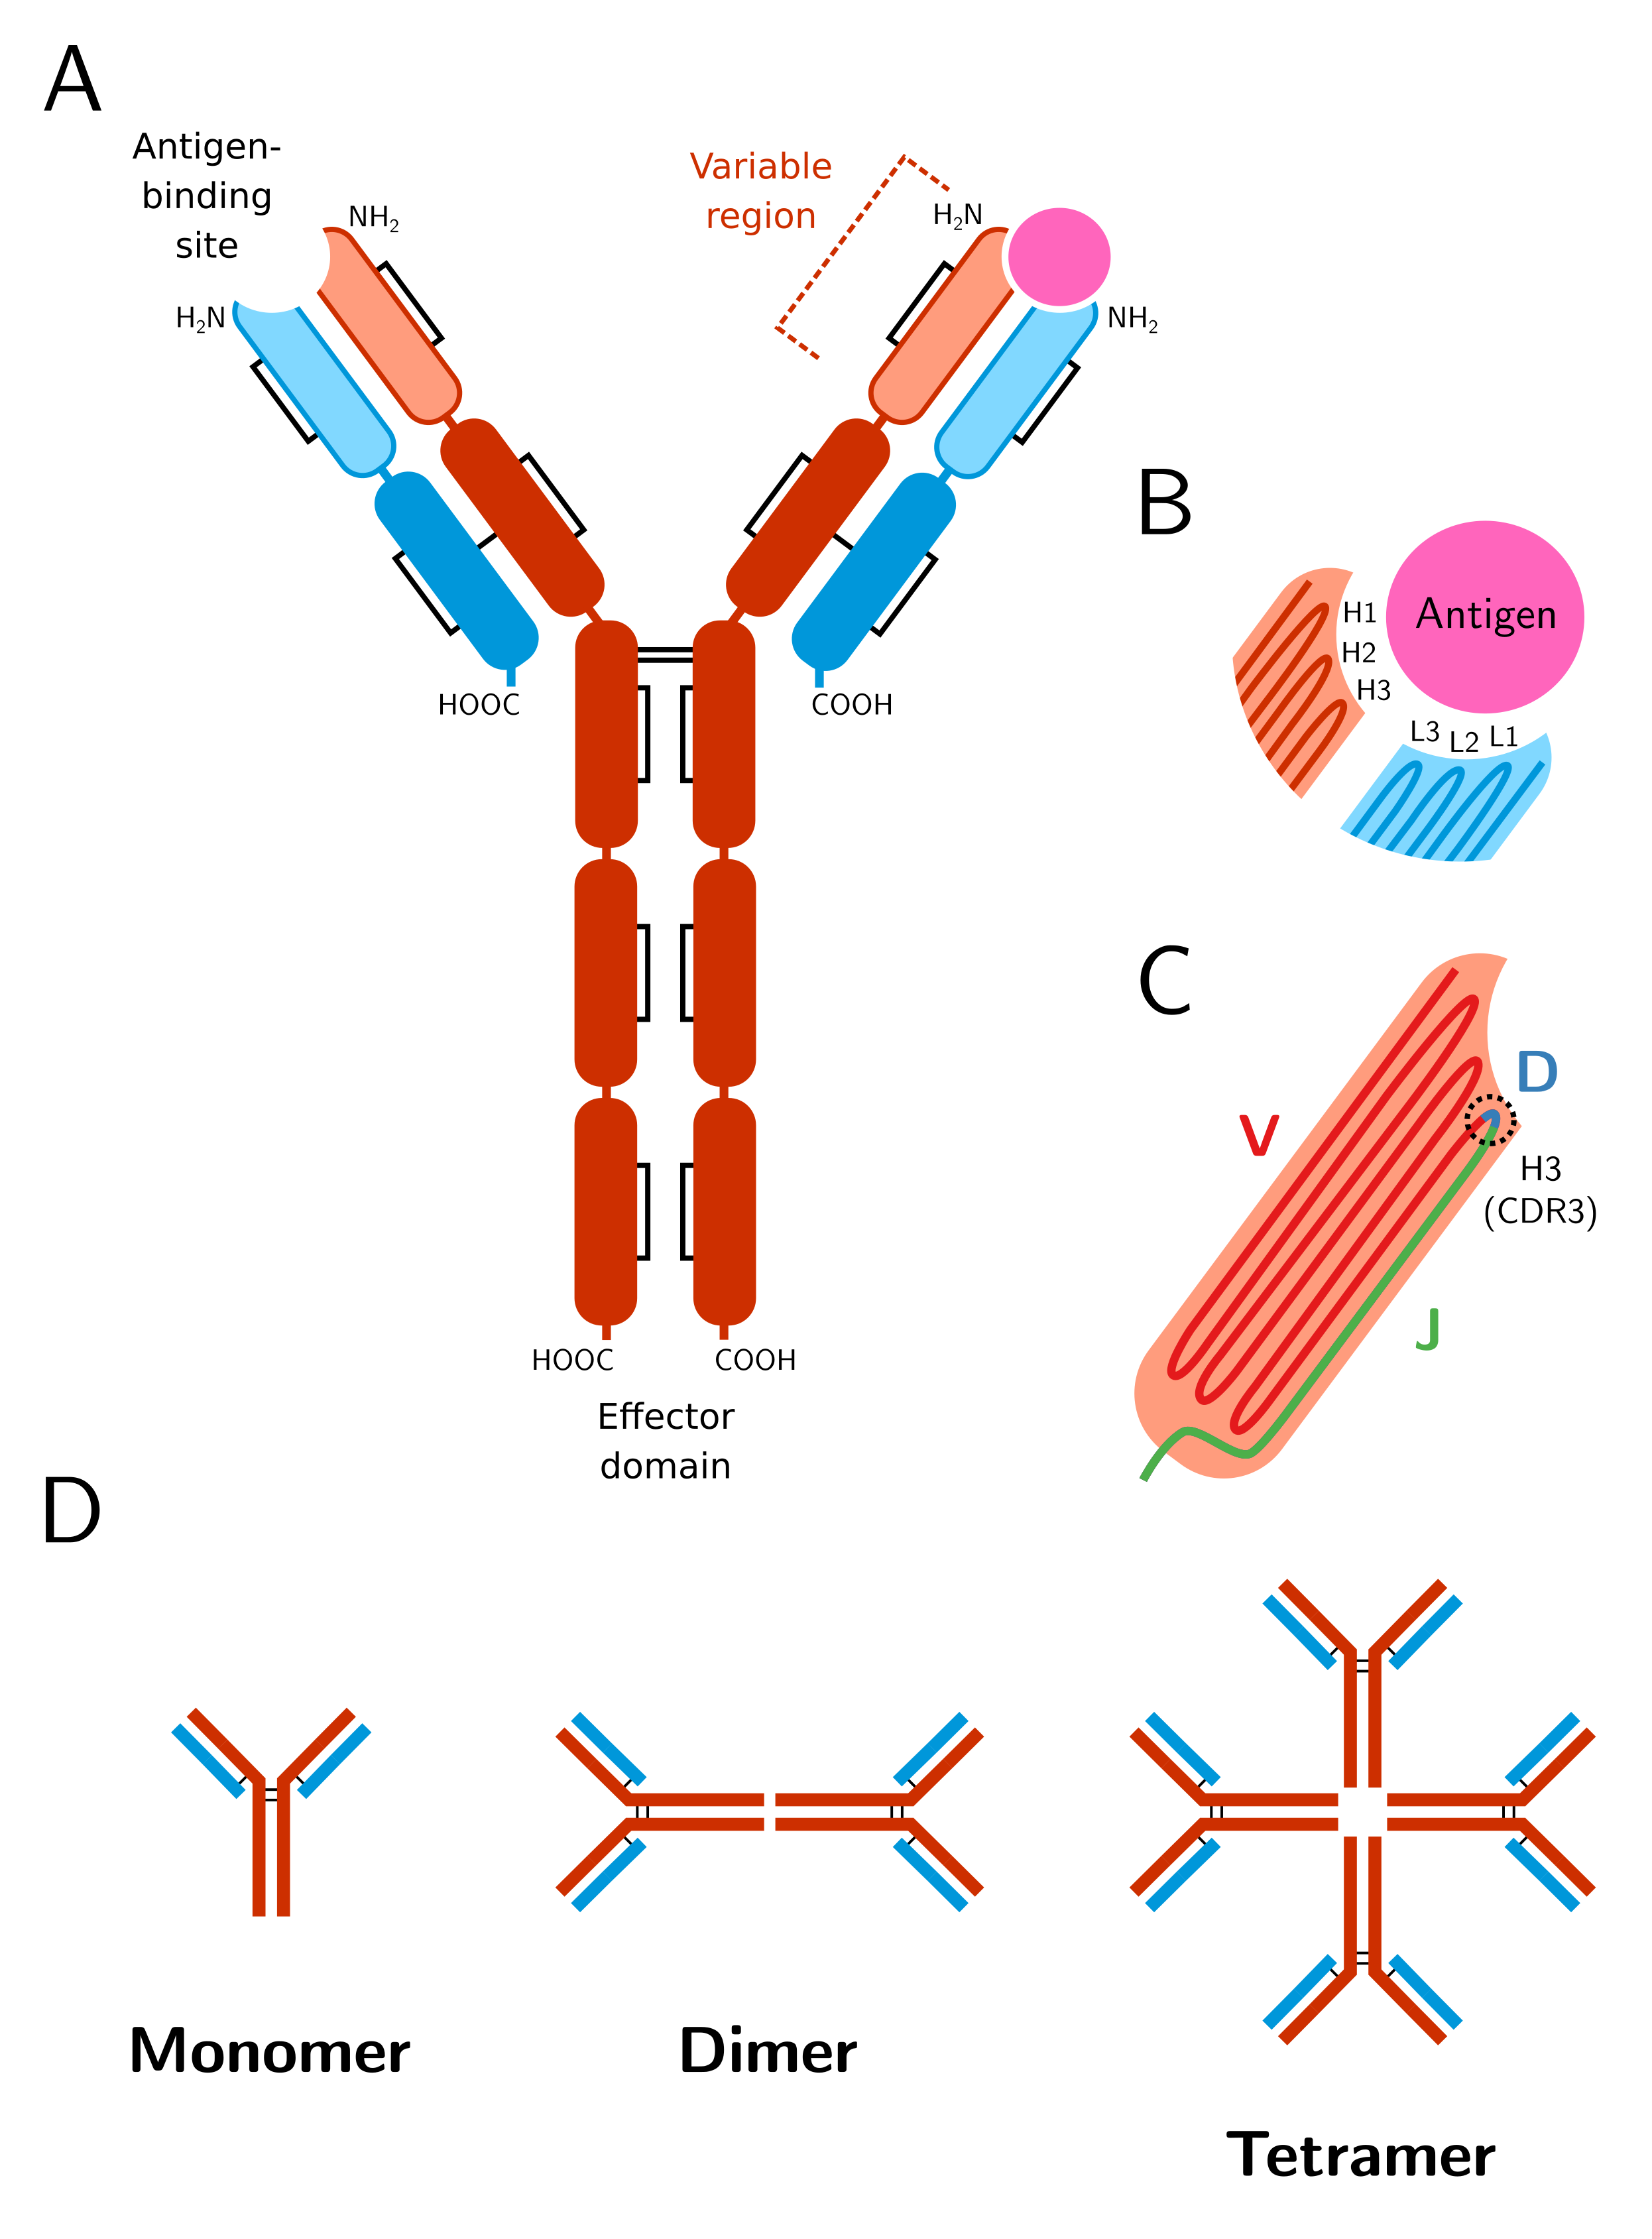
\includegraphics[width=0.9\textwidth]{_Figures/png_edited/antibody-structure}
\begin{subfigure}{0em}
\phantomsubcaption{}
\label{fig:intro-antibody-structure-schematic}
\end{subfigure}
\begin{subfigure}{0em}
\phantomsubcaption{}
\label{fig:intro-antibody-structure-loops}
\end{subfigure}
\begin{subfigure}{0em}
\phantomsubcaption{}
\label{fig:intro-antibody-structure-vdj}
\end{subfigure}
\begin{subfigure}{0em}
\phantomsubcaption{}
\label{fig:intro-antibody-structure-multimers}
\end{subfigure}
\caption[Antibody structure and function]{\textbf{Antibody structure and function:} (A) Schematic of a hingeless secreted antibody monomer, with heavy chains depicted in red, light chains in blue, and bound antigen in pink. Immunoglobulin fold domains are depicted as rounded rectangles, with variable-region domains shown with light shading and constant-region domains with dark. Black lines indicate disulfide bonds. (B) Schematic close-up of an immunoglobulin antigen-binding site, indicating the six loop regions (H1-3 and L1-3) making up the antigen-binding region. (C) Schematic close-up of the heavy-chain variable region, indicating the regions corresponding to the variable, diversity and joining gene segments from the unrecombined \igh{} locus. Note the chimeric nature of the third antigen-binding loop (H3, marked), which is formed by parts of all three gene segments. (D) In the context of antibodies, ``monomer'' refers to a single four-chain antibody protein, while ``dimer'', ``tetramer'' \etc refer to multiple antibodies linked together through covalent or noncovalent interactions.}
\label{fig:intro-antibody-structure}
\end{figure}
% TODO: Actual antibody crystal structure here?

\subsection{Antibody sequence diversification and primary repertoire diversity}
\label{sec:intro_immunity_primary}

% TODO: Discuss allelic exclusion (Magadan)
% TODO: Read up on allelic exclusion in teleosts in Magadan 2015

The immune environment encountered by a vertebrate organism contains an enormous number of different potential pathogenic threats, each of which has its own antigenic signatures and many of which are capable of evolving much more rapidly than the vertebrate host \parencite{jack2015evolution}. In order for the adaptive immune system to cope with this huge diversity of different threats, it must be able to produce antibodies with a correspondingly large diversity of different antigen specificities. The greater the potential diversity of antibody sequences available to the adaptive immune system, the greater its capacity to respond effectively to novel immune threats. In reality, the mechanisms employed by the vertebrate adaptive immune system to diversify its antigen receptors enable an almost unlimited diversity of potential antibody sequences, with a correspondingly vast array of potential antigen specificities \parencite{mora2016quantifying}.

The mechanisms by which the adaptive immune system produces this diversity are dramatic, and rely on a highly unusual underlying gene structure \parencite{jung2006vdjr} and a very high level of cellular wastage \parencite{kogut2012bcells}. In the humoral immune system, antibody diversification takes place during B-cell development in the primary lymphopoietic organs (bone marrow in mammals, anterior kidney in teleosts \parencite{sunyer2013fishing}). Prior to this process, the native antibody loci in B-progenitor cells (and other cell types) is highly fragmented \parencite{jung2006vdjr}, with numerous fragmentary variable-region sequences present in series on the chromosome upstream of the constant-region exons. In the heavy chain locus, these variable-region gene segments can be divided into three categories:

\begin{itemize}
\item \textbf{Variable (\vh) segments} are the longest class of gene segment, at roughly \bp{300} in length. Each V-segment codes for the majority of the variable region of an antibody, including the entirety of the first three framework regions (FWR1-3) and the first two complementarity-determining regions (CDR1-2) as well as the 5' part of CDR3 \parencite{jung2006vdjr} (\Cref{fig:intro-antibody-structure-vdj}). They are therefore highly structured, and include several highly-conserved positions present in virtually all functional V-segments in nearly all species, including two conserved cysteine residues (which code for an intra-domain disulfide bond) and a conserved tryptophan residue following CDR1 \parencite{lefranc2003vnumbering}. Each V-segment is also associated with its own promoter sequence and 5'-UTR, as well as a 5'/C-terminal leader peptide between the translation start site and the start of the functional V-sequence.
\item \textbf{Diversity (\dh) segments} are the shortest class of segment, typically on the order of 10-\bp{20}, and are the least structured \parencite{ruiz1999humandj}. They form the middle part of CDR3 (\Cref{fig:intro-antibody-structure-vdj}) \parencite{schroeder2010immunoglobulins}.
\item \textbf{Joining (\jh) segments} are of intermediate length, typically 50-\bp{60} \parencite{ruiz1999humandj}. They form the 3'/C-terminal part of heavy chain CDR3 and the 5'/N-terminal part of FR4 (\Cref{fig:intro-antibody-structure-vdj}) \parencite{schroeder2010immunoglobulins}. Each J-segment is succeeded on the chromosome by a splice donor site \parencite{magadan2011medaka}, which is used to join the variable region of the antibody sequence to the constant region via RNA splicing following transcription of \igh{} mRNA (\Cref{fig:intro-vdjr-locus}iii). Like \vh segments, \jh segments can be identified from their conserved structure, particularly the conserved tryptophan residue marking the end of CDR3 \parencite{ruiz1999humandj}.
\end{itemize}

In the simplest ``translocon" configuration of the \igh{} locus, blocks of repeated \vh, \dh and \jh segments are present in series on the chromosome in contiguous V-, D- and J-regions (\Cref{fig:intro-vdjr-locus}i) \parencite{schroeder2010immunoglobulins,jung2006vdjr}. During B-cell development, a single \vh, \dh and \jh segment are selected, and the intervening genomic regions are permanently excised from the genome to produce a single contiguous VDJ sequence coding for the complete variable region of an antibody (\Cref{fig:intro-vdjr-locus}ii). The mechanism by which this excision occurs is called VDJ recombination, and relies on a specialised recombinase complex containing lymphocyte-specific recombination-activating genes 1 and 2 (\gene{RAG1} and \gene{RAG2}) \parencite{jung2006vdjr,schatz2011vdjr}. This complex recognises specialised recombination signal sequences (RSSs) flanking each variable gene segment, composed of highly conserved heptamer and nonamer sequences separated by a spacer sequence of conserved length (either 12 or \bp{23}, corresponding respectively to one or two turns of the DNA helix) \parencite{hesse1989rss} (\Cref{fig:intro-vdjr-consensus}). Each functional \vh segment is succeeded by a \bp{23}-spacer RSS in 5'-3' orientation, while each \jh segment is preceded by a \bp{23}-spacer RSS in 3'-5' orientation; each \dh segment, meanwhile, is flanked by \bp{12}-spacer RSSs in 5'-3' and 3'-5' orientation, respectively (\Cref{fig:intro-vdjr-rss}) \parencite{schatz2011vdjr}. 

In VDJ recombination, recombinase complexes bind two of these RSSs and associate with each other to bring the two corresponding gene segments into close proximity (\Cref{fig:intro-vdjr-mechanism}i-iii). A single-strand DNA nick is introduced between each RSS and its gene segment, and the exposed 3'-hydroxyl group of the break attacks the 5'-phosphate on the other strand to produce an asymmetric double-strand break, with the coding sequence terminating in a hairpin loop and the cleaved RSS in a blunt end \parencite{schroeder2010immunoglobulins,schatz2011vdjr} (\Cref{fig:intro-vdjr-mechanism}iv-v). These breaks are then resolved by the ubiquitous non-homologous end-joining machinery of the DNA damage response: the blunt ends of the cleaved RSSs can be directly ligated together, while for the coding sequences the hairpin loops must first be cleaved and the resulting 3'-overhangs resolved \parencite{schroeder2010immunoglobulins,schatz2011vdjr} (\Cref{fig:intro-vdjr-mechanism}vi-vii). The net result of this process is a contiguous V/D or D/J join in the coding sequence and a ligated DNA circle containing the excised RSSs and intervening sequence, which is subsequently degraded. Via unknown mechanisms \parencite{schatz2011vdjr}, the recombination machinery exhibits a strong preference for RSS sequences of different lengths (the so-called ``12/23 rule''), encouraging  D-J and V-D joins while largely preventing V-J joins. 

The simple joining of gene segments during VDJ recombination provides a basic combinatorial sequence diversity, with a number of possible sequences in the simplest case equal to the product of the numbers of \vh, \dh and \jh segments in the \igh{} gene locus. The number of potential \igh{} variable-region sequences in most species, however, is vastly higher than this: in humans, for example, there are roughly 8000 possible functional VDJ combinations \parencite{lefranc2001humanheavy}, but the number of different possible nucleotide sequences exceeds $10^{22}$ \parencite{elhanati2015model}. This huge difference arises from the inexactness with which the coding ends produced by the recombinase complex are joined following RSS excision (\Cref{fig:intro-vdjr-junctions}). Before the two gene segments brought together in VDJ recombination can be joined by NHEJ, the hairpin loops formed by the recombinase complex must be resolved by re-nicking the DNA \parencite{schroeder2010immunoglobulins,schatz2011vdjr}. This re-nicking process is not exact, and often occurs within the coding sequence, resulting in a palindromic 3'-overhang that can be filled in (resulting in palindromic \textit{P-insertions}) or trimmed (resulting in \textit{deletions}). The resulting blunt ends then serve as substrates for the lymphocyte-specific terminal dideoxy transferase enzyme (TdT), which adds a variable number of untemplated nucleotides (nonpalindromic \textit{N-insertions}) prior to sequence ligation \parencite{schroeder2010immunoglobulins,schatz2011vdjr}. As a result, the final recombined sequence is frequently not a clean ligation of the two original gene segments, but an inexact join involving multiple missing terminal positions and/or \textit{de novo} inserted sequence, a phenomenon collectively known as \textit{junctional diversity} (\Cref{fig:intro-vdjr-mechanism}vi-vii) \parencite{flaherty2012chapter}.

The three process contributing to junctional diversity (P insertion, N insertion, and deletion) together vastly increase the potential antibody sequence diversity available to a developing B-cell at the heavy-chain CDR3 region, which as a consequence is by far the most variable single region in determining antigen specificity \parencite{shirai1999h3}. This junctional diversity, however, comes at a substantial cost. The indel mutations introduced by VDJ recombination are not constrained to occur in multiples of three over both junctions, resulting in a high rate of recombinations in which the \vh and \jh segments are out of frame with each other; still more loci are rendered nonfunctional through the introduction of \textit{de novo} STOP codons. As the sequence changes introduced by VDJ recombination are irreversible, many developing B-cells are left with permanently disrupted \igh{} loci on both chromosomes, and are left with no recourse but programmed cell death. In addition, the huge and untemplated sequence diversity introduced in this way means that many B-cells whose \igh{} loci do successfully undergo VDJ recombination are left with BCRs that either cannot effectively bind any antigen or strongly bind self-antigen, resulting in useless antibodies in the first case and a dangerous risk of autoimmunity in the second; these B-cells are eliminated through a process of antigenic selection before \naive B-cells are permitted to exit the primary lymphopoietic organs, resulting in still more wastage as cells with nonfunctional or self-binding antigens undergo programmed cell death. Overall, as many as 90\% of developing B-cells may be eliminated by one or other of these processes before successfully exiting the primary lymphoid organs \parencite{kogut2012bcells}.  

% More details on primary selection in Kogut and its sources if needed

Taken together, the processes of VDJ recombination, junctional diversity and primary selection will produce a population of \naive B-cells with an extremely high diversity of heavy-chain ideotypes, with virtually every \naive B-cell expressing a unique variable-region sequence. Taken together, the resulting population of sequences represents the \textit{primary antibody heavy-chain repertoire} of the organism, and determines the range of different antigen sequences the humoral immune system of that organism can potentially respond to. The diversity of this primary repertoire depends on the native structure of the \igh{} locus in that species (which determines the number of segment choices available to the VDJ-recombination process), the distribution of possible numbers of insertions or deletions contributing to junctional diversity, and the stringency of the primary selection process.

\begin{figure}
\centering
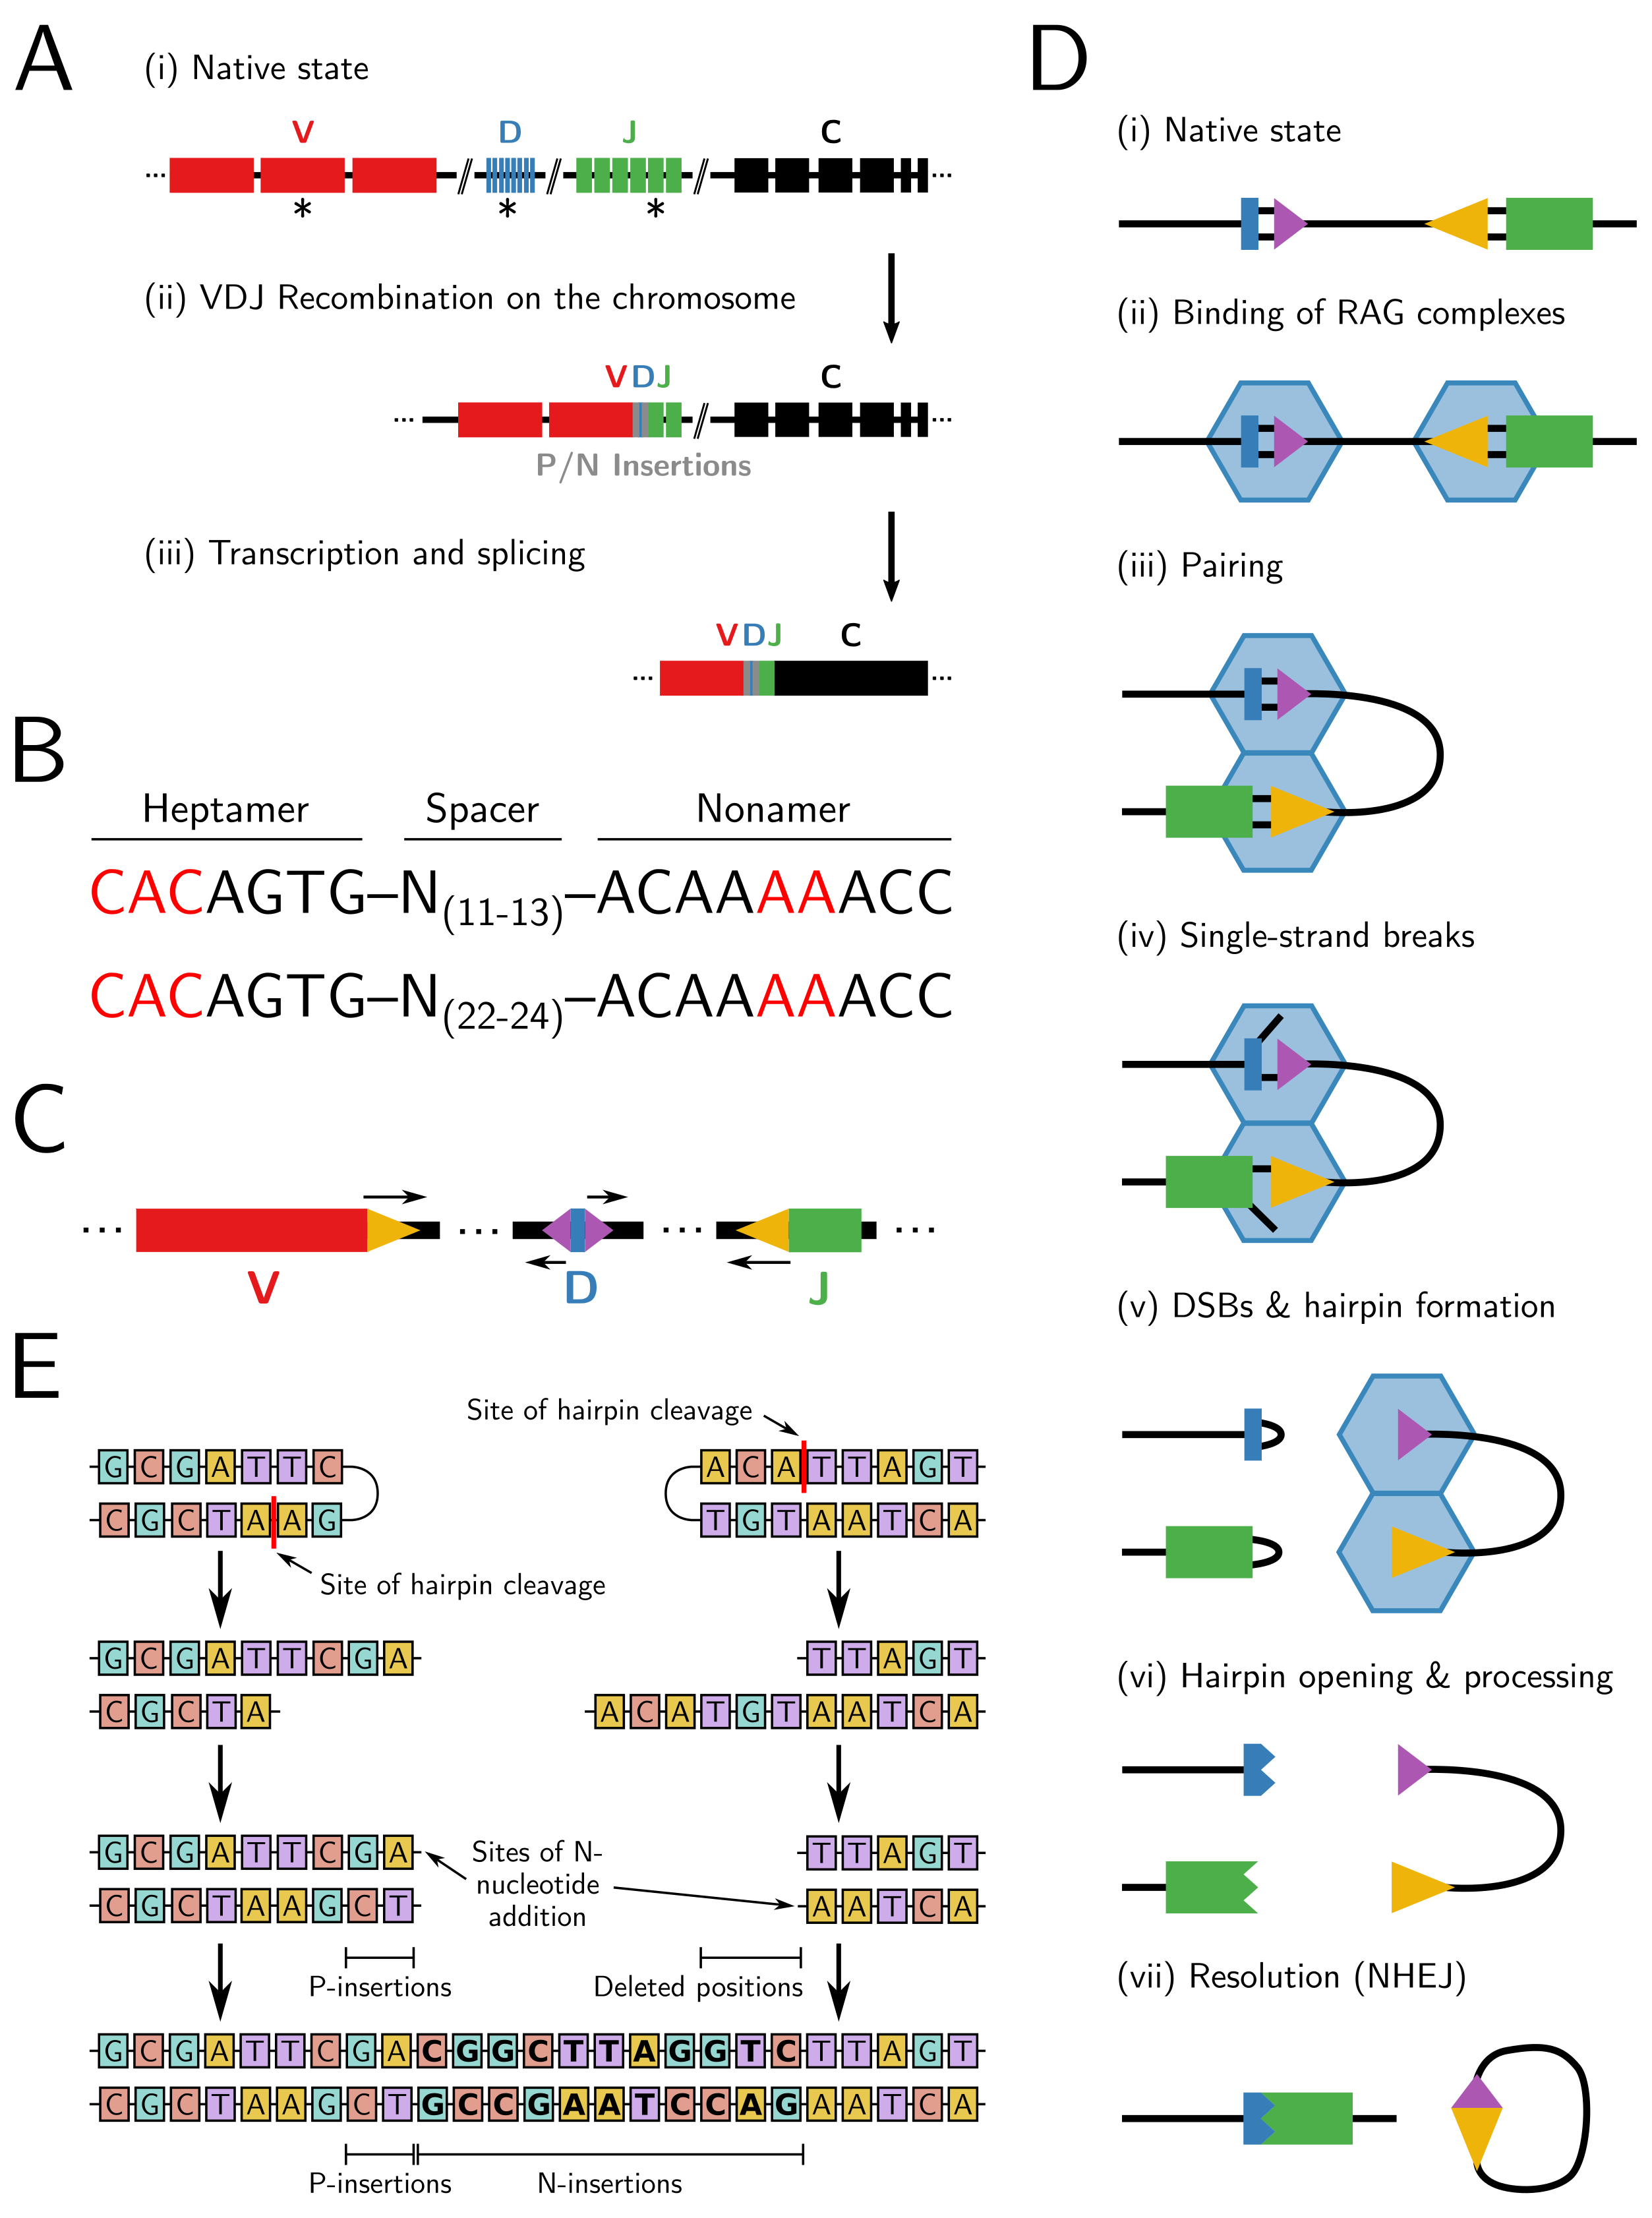
\includegraphics[width=0.95\textwidth]{_Figures/png_edited/primary-diversity}
\begin{subfigure}{0em}
\phantomsubcaption{}
\label{fig:intro-vdjr-locus}
\end{subfigure}
\begin{subfigure}{0em}
\phantomsubcaption{}
\label{fig:intro-vdjr-consensus}
\end{subfigure}
\begin{subfigure}{0em}
\phantomsubcaption{}
\label{fig:intro-vdjr-rss}
\end{subfigure}
\begin{subfigure}{0em}
\phantomsubcaption{}
\label{fig:intro-vdjr-mechanism}
\end{subfigure}
\begin{subfigure}{0em}
\phantomsubcaption{}
\label{fig:intro-vdjr-junctions}
\end{subfigure}
\caption[Primary sequence diversification in antibodies]{\textbf{Primary sequence diversification in antibodies:} (A) Schematic of antibody sequence formation at the locus level. Black asterisks indicate the segments to be recombined. (B) Consensus sequence of short (above) and long (below) RSSs in jawed vertebrates. Nucleotides marked in red are the most strongly conserved and most required for efficient recombination \parencite{hesse1989rss}. (C) Schematic of position and orientation of long (orange) and short (purple) RSSs relative to variable-region gene segments. (D) Schematic of recombination mechanism for a D/J segment pair, illustrating hairpin formation and imprecise end-joining of coding sequences; adapted from \parencite{schatz2011vdjr}, Figure 2. (E) Example of the inexact hairpin resolution mechanisms leading to junctional diversity in (D-vi); adapted from \parencite{flaherty2012chapter}, Figure 10-5.
} 
\label{fig:intro-vdjr}
\end{figure}


%VDJ recombination in the \textit{IGH} locus is highly structured, and occurs in a specific order. First, a D and a J segment are selected and recombined to produce a DJ sequence. Then, a V region is selected and recombined with the DJ to produce a continuous VDJ sequence constituting the variable region of the heavy chain. The complete protein sequence is produced during later transcriptional splicing, which joins this variable-region sequence to downstream constant-region exons to produce a mature \textit{IGH} mRNA. This strict ordering of V/D/J segments, which obtains in the vast majority of recombined sequences observed, is produced through the combination of a variety of regulatory mechanisms. The most basic of these is the structure of the RSSs, which comprise a conserved heptamer and nonamer sequence separated by a relatively unconserved spacer region of either 12 or 23bp \parencite{jung2006vdjr}, corresponding to either one or two turns of the DNA helix. V and J segments in the IGH locus are flanked by RSSs with 23bp spacer regions, while those flanking D-regions have 12bp spacers %citation needed
%As the RAG recombinase specifically recognises pairs of RSSs with dissimilar spacer lengths (a restriction known as the 12/23 or one-turn/two-turn rule), direct V-to-J recombination events are excluded \parencite{jung2006vdjr}. % Better citation if possible.
%
%Complete VDJ recombination places the V-region promoter in close proximity to a highly-conserved enhancer element (known as iE$\mu$) lying between the last J segment and the first constant-region exon \parencite{jung2006vdjr}; this enhancer is important for strong expression of the mature IGH mRNA from the pre-B-cell stage onwards. 

\subsection{\igh{} locus structure in teleost fishes}
\label{sec:intro_teleost_loci}

\Cref{sec:intro_immunity_primary} describes the process of \igh{} locus maturation in terms of an idealised translocon locus with a simple V-D-J-C structure (\Cref{fig:intro-vdjr-locus}). In some species, including humans and mice, \igh{} loci roughly correspond to this simplified structure, albeit with a much larger number of gene segments; however, in many species, including all teleosts, this idealised structure is a significant oversimplification of the actual layout of their \igh{} loci \parencite{fillatreau2013astonishing}. Due to their repetitiveness and complex structure, comprehensive assembly of \igh{} loci is often difficult, and full elucidation of their structure often requires a focused characterisation effort. Nevertheless, a number of teleost loci have been characterised to date, including several species (e.g. three-spined stickleback and medaka) closely related to the African turquoise killifish.

Among teleost fishes, the simplest \igh{} locus structures known to date are exhibited by species such as zebrafish, grasscarp, and fugu (\Cref{fig:intro-teleost-loci-simple}) \parencite{fillatreau2013astonishing}. In these species, the \igh{} locus adopts a V-D-J-\cz{}-D-J-\cm{}-\cd{} structure, with a single shared V-region followed by D- and J-regions specific to the \igh{Z} and \igh{M/D} constant regions, respectively. The rainbow trout locus has a similar organisation, but with two additional V-segments following the \igh{Z} region \parencite{hansen2005trout}. During VDJ recombination in these loci, the choice of variable gene segments also determines the choice of constant region: if a pair of \dh and \jh segments upstream of the \igh{Z} constant region is selected, the cell will express \igh{Z}, while if the segments chosen are downstream of \igh{Z}, that constant region will be excised during VDJ recombination and \igh{M} and/or \igh{D} will be used instead. As a result, VDJ recombination in these species determines both the ideotype of a developing B-cell and its isotype \parencite{fillatreau2013astonishing}.

While some teleost species possess such relatively simple \igh{} loci, many species exhibit much more complicated, and often much larger, locus structures. In many species, multiple distinct subloci (comprising V-, D- and J-regions and least one constant region) are present in tandem on the chromosome, often with distinct combinations of variable gene segments and constant regions (\Cref{fig:intro-teleost-loci-complex}); in a few cases, such as medaka and Atlantic salmon, one or more of these subloci is in inverted orientation relative to the rest of the locus. In some species, such as Atlantic salmon, whole-genome duplication has led to the existence of multiple distinct \igh{} loci on different chromosomes, each of which has its own complement of subloci, gene segments, and constant regions \parencite{yasuike2010salmon}. In this milieu, pseudogenisation of gene segments or constant-region exons is common, resulting in loci with large numbers of pseudogenised V-segments and constant regions.

The diversity in locus size and organisation among teleost fishes is likely to have important consequences for humoral adaptive immunity in these species. The native locus constitutes the raw substrate for the VDJ recombination process, and the number of different \vh, \dh and \jh gene segments available for recombination defines the baseline sequence diversity of antibodies in that species. It is not clear to what extend VDJ recombination can take place across different subloci in the large tandem loci described in \Cref{fig:intro-teleost-loci-complex}; if recombination between subloci is restricted, this will also have important effects on the kinetics of VDJ recombination in a species. The division of an \igh{} locus into tandem subloci may also have effects on the statistics of B-cell maturation, with more subloci conceivably presenting the opportunity for a greater number of recombination attempts before the \igh{} loci of a developing B-cell are exhausted and so reducing the rate at which cells fail to mature successfully; however, to my knowledge little or nothing is known about the effects of locus structure on B-cell developmental processes at present. Finally, variations in the constant regions present in different species are likely to have very important effects on humoral immunity; most fundamentally, whereas \igh{Z/T} appears to be specialised for mucosal adaptive immunity in those teleost species that possess it \parencite{zhang2010igtgut,fillatreau2013astonishing,xu2013igtskin}, it is not known how mucosal immune responses manifest in species lacking this isotype. Given all these important (and potentially-important) effects of \igh{} locus structure on humoral adaptive immunity, characterising the sequence and organisation of this locus is an essential step in understanding the adaptive immune system of any vertebrate species.

\begin{figure}
\centering
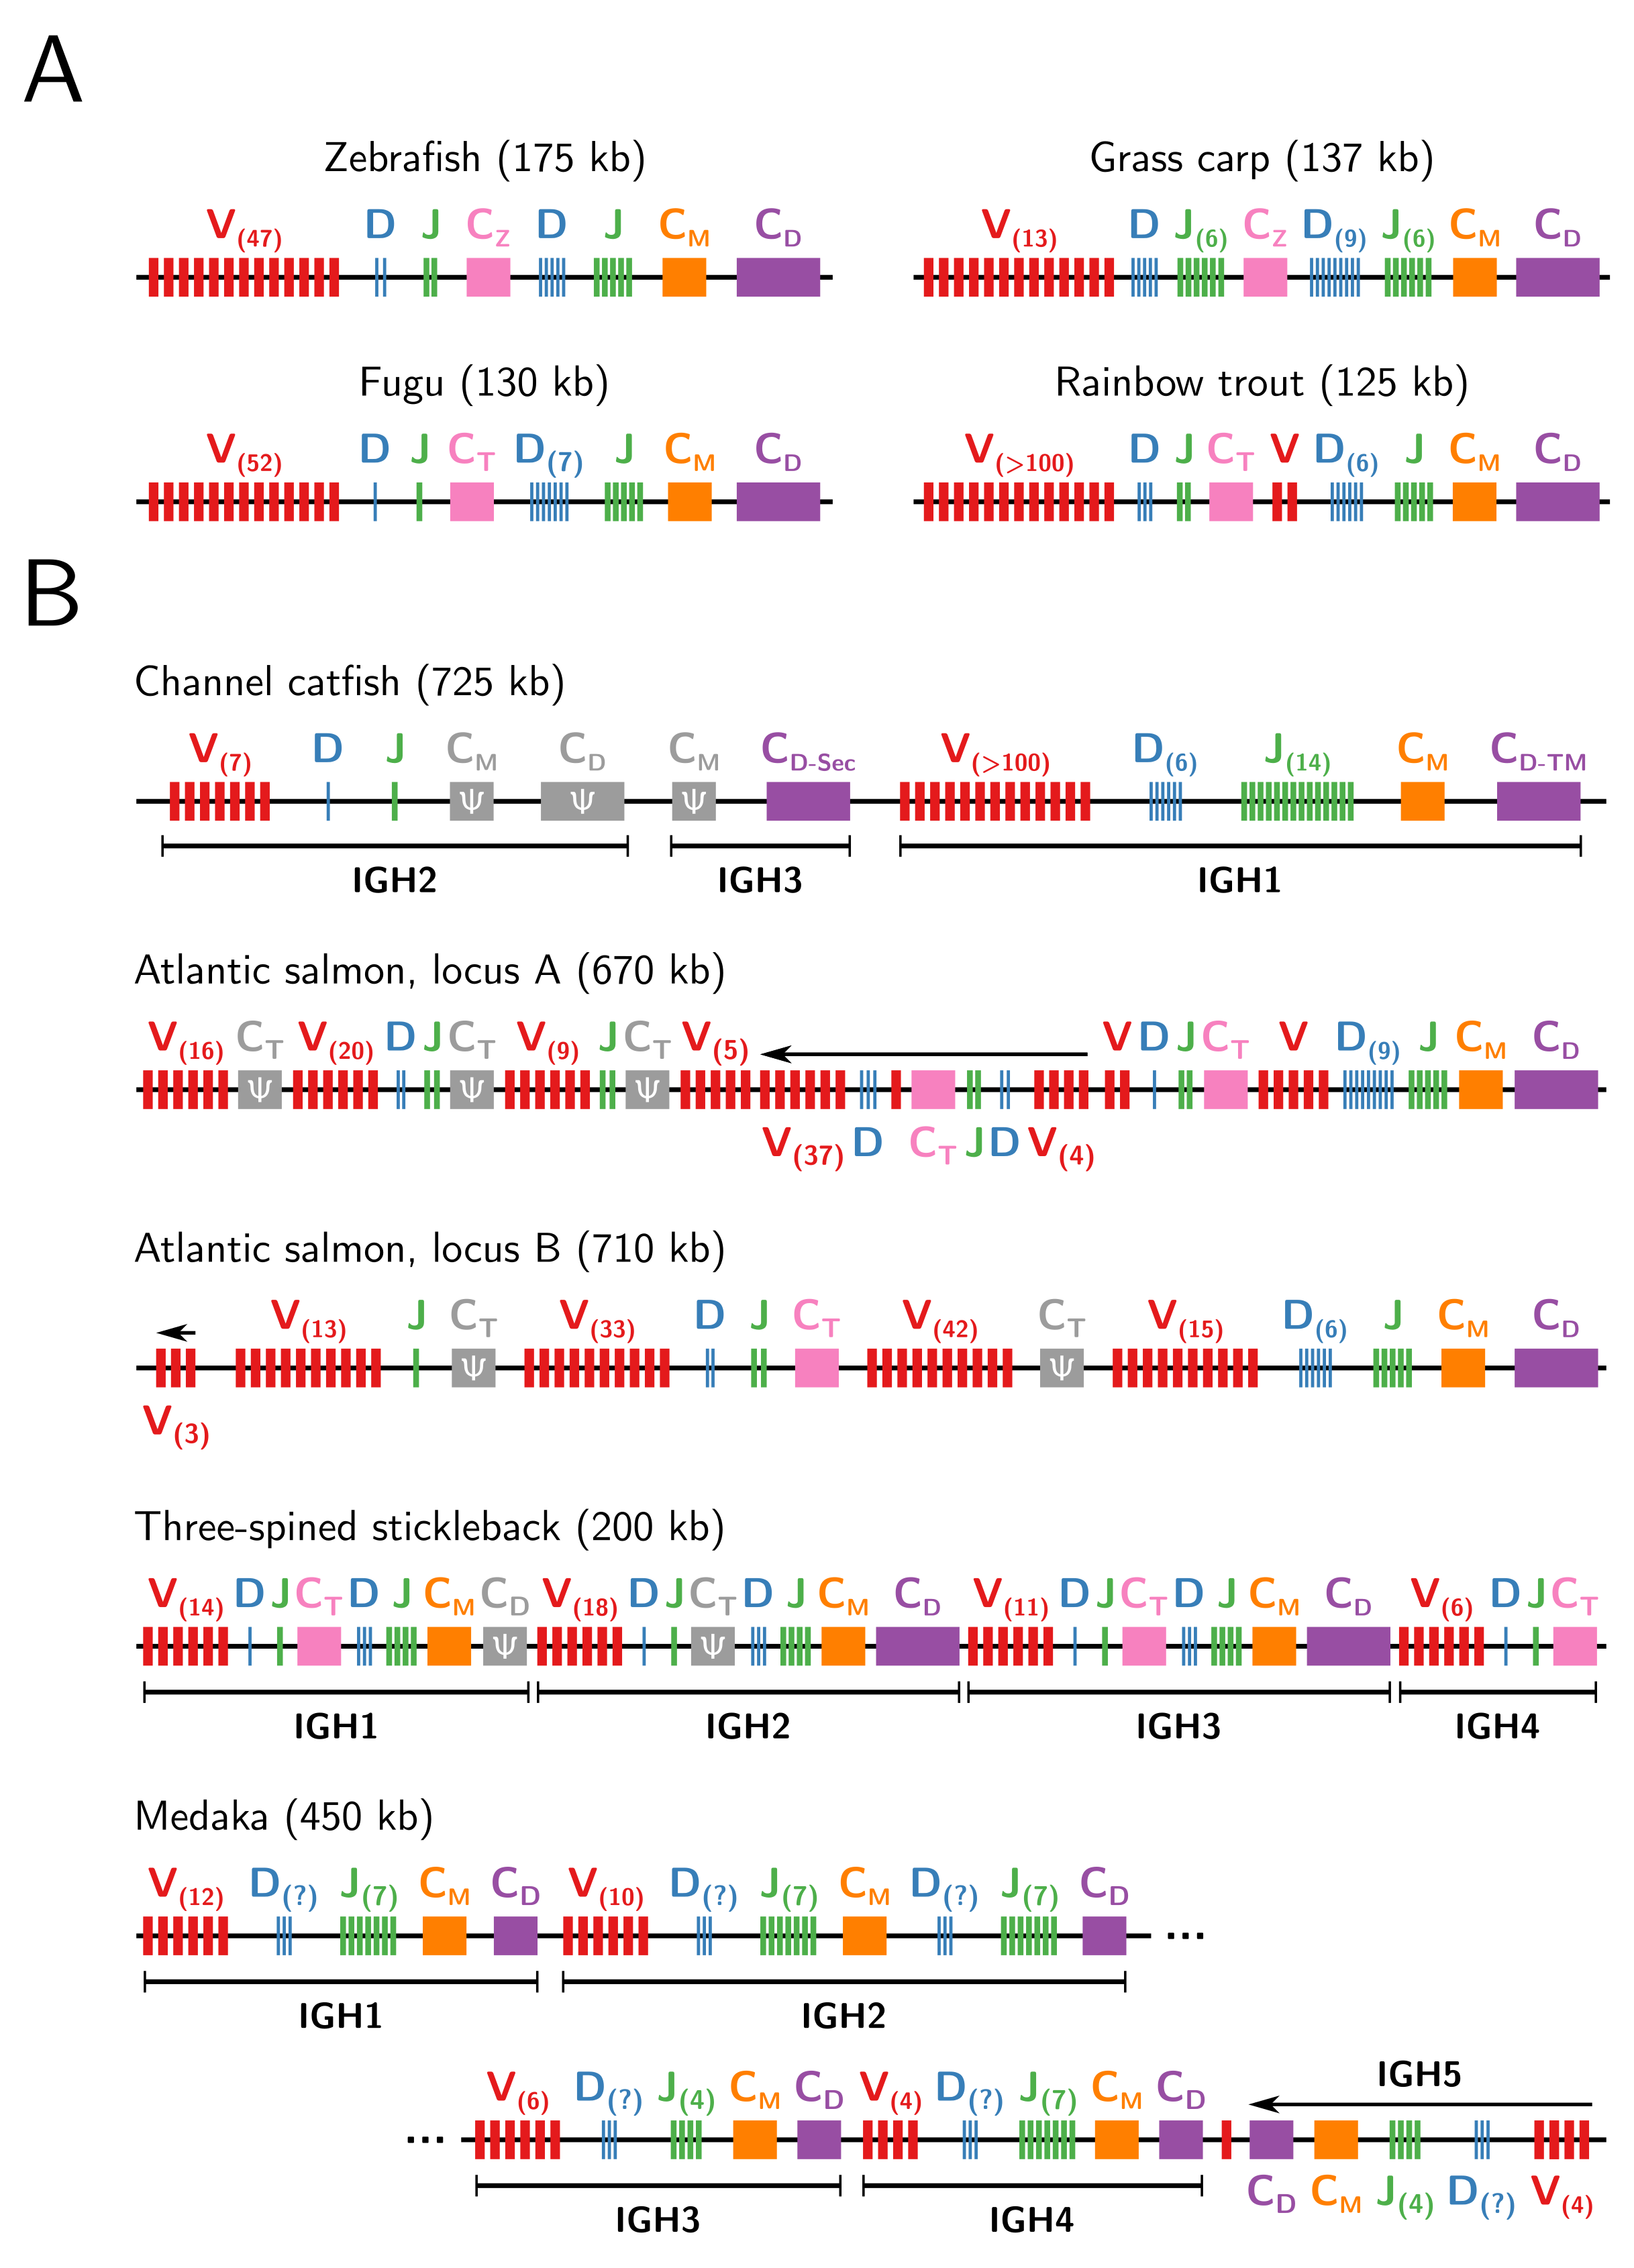
\includegraphics[width=0.85\textwidth]{_Figures/png_edited/teleost-loci}
\begin{subfigure}{0em}
\phantomsubcaption{}
\label{fig:intro-teleost-loci-simple}
\end{subfigure}
\begin{subfigure}{0em}
\phantomsubcaption{}
\label{fig:intro-teleost-loci-complex}
\end{subfigure}
\caption[\igh{} locus structure in teleost fishes]{\textbf{\igh{} locus structure in teleost fishes:} Simplified schematics of \igh{} loci from nine teleost species. (A) In the simplest teleost \igh{} loci, single \igh{Z} and \igh{M/D} constant regions share a common V-region, but are preceded by separate D/J regions. In rainbow trout, a small number of V-segments also separate \igh{Z} from the pre-\igh{M} D-region. (B) In many teleosts, the \igh{} loci are much larger and more complex, with repeated tandem subloci (labelled regions), pseudogenised constant regions (grey, $\psi$), inverted segments (leftward arrows), and other deviations from the classic locus organisation. Loci are not to scale; blocks of more than five segments are condensed and labelled with their segment number, as are some smaller segment blocks for clarity. Adapted from \parencite{fillatreau2013astonishing}, Figure 2 and \parencite{bengten2015fishantibodies}, Figure 4, with additional information from \parencite{magadan2011medaka,bao2010stickleback,gambondeza2011stickleback,yasuike2010salmon,xiao2010grasscarp}.
The number of D-regions in the medaka locus is not provided in the sources.}
\label{fig:intro-teleost-loci}
\end{figure}

\subsection{Affinity maturation and secondary repertoire diversity}
\label{sec:intro_affinity_maturation}

Following VDJ recombination and primary selection, developed \naive B-cells emerge from the primary lymphoid organs and circulate in the periphery. At some point, a subset of these \naive cells will make contact with their cognate antigen. If this contact occurs in the correct signalling context (in particular, in the presence of T-cell help), the B-cell becomes activated and begins to proliferate \parencite{dunnwalters2010bcellageing}. During this clonal expansion process, the B-cell's antibody genes undergo a very high rate of somatic mutation (known as \textit{somatic hypermutation} or SHM), with mutations focused in the complementarity-determining regions coding for the antigen-binding loops of the variable region; in mammals, the rate can be as high as $10^{-3}$ per nucleotide per cell division \parencite{noia2007shm}. This SHM process is orchestrated by the activation-induced cytidine deaminase enzyme (AID), which preferentially targets particular hotspot motifs (canonically  RGYW/WRCY and WA/TW) and deaminates cytidine residues to uracil, which can either be corrected to thymine on DNA replication (resulting in a C-to-T transition mutation) or removed via base-excision repair (resulting in a variety of other mutations) \parencite{magor2015affinity}. As a result, the original antibody sequence of the ancestral \naive cell is diversified into a cluster of related sequences, with widely varying affinity for the cognate antigen.

In order for the combination of clonal expansion and somatic hypermutation to improve the adaptive immune system's ability to respond to the stimulating antigen, the resulting clone needs to undergo a selection process, to identify and advantage cells expressing antibodies with improved antigen affinity. This selection is effected through a competitive process in which clonally-expanded B-cells attempt to bind cognate antigen trapped on the surface of helper cells: those cells which successfully bind antigen receive growth and differentiation signals, while those which do not undergo programmed cell death. In mammals, this process takes place primarily in histologically-distinct germinal centres within specialised secondary lymphoid organs such as the spleen \parencite{howard2006quality,noia2007shm}, in which B-cells that have encountered antigen first undergo clonal expansion and SHM, then compete for antigen on the surface of follicular dendritic cells \parencite{howard2006quality}. In teleosts, which lack specialised, histologically-differentiated germinal centres, B-cell proliferation takes place near clusters of melanomacrophages surrounded by reticular cells, both of which have been attributed an antigen-trapping and -presentation role analogous to that performed by FDCs in mammals \parencite{magor2015affinity}.

While clonal expansion, somatic hypermutation and clonal selection, collectively known as \textit{affinity maturation}, are present in both mammals and teleosts, the increase in antibody affinity resulting from this process in teleosts is far weaker than in mammals (e.g. 3-to-10-fold in rainbow trout, compared to as much as 1000-fold in mammals \parencite{magor2015affinity}). Since SHM appears to be fully functional in those fish so far investigated (albeit with a greater bias towards C-to-T transitions over other mutations) \parencite{magor2015affinity}, this difference seems likely to arise from differences in clonal selection dynamics between teleosts and mammals. The reasons for such a difference are still not entirely clear, but may involve histological differences in where and how affinity maturation takes place in these taxa. In mammalian germinal centres, the ratio between expanded B-cells and FDCs is such that the amount of presenting antigen is limiting, forcing competition for antigen among B-cells and favouring those cells which can bind antigen most strongly \parencite{magor2015affinity}. In teleosts, conversely, proliferating B-cells are far outnumbered by antigen-trapping melanomacrophages and reticular cells, resulting in an oversupply of antigen relative to B-cell demand; this antigen surplus may result in faster overall proliferation, but at the cost of much weaker selection for high-affinity antibodies \parencite{magor2015affinity}.

Following affinity maturation, activated B-cells undergo differentiation into memory cells (which persist in the bloodstream for long periods and provide secondary immune memory) and plasmablasts/plasma cells (which secrete large amounts of antigen to mount a powerful immune response) \parencite{howard2006quality,dunnwalters2010bcellageing}. Affinity-matured cells can also re-enter germinal centres (or their less-developed teleost equivalents) to undergo additional rounds of proliferation, hypermutation and selection \parencite{howard2006quality}; memory cells can also undergo further rounds of affinity maturation, resulting in even larger and more diverse clones and still-higher levels of antigenic affinity. In tetrapods, class switching between different constant-region isotypes also occurs as part of affinity maturation, and is also orchestrated by AID; however, this process is absent in teleosts \parencite{magor2015affinity}.

The combination of the primary (\naive) repertoire described in \Cref{sec:intro_immunity_primary} with the clonal expansions and additional sequence diversity arising from affinity maturation constitutes the \textit{secondary heavy-chain antibody repertoire} of the organism (\Cref{fig:intro-bcell-repertoires}). This is the repertoire actually encountered by incoming pathogens and available to relatively direct experimental interrogation. The structure and diversity of this secondary repertoire depends on the makeup of the primary repertoire, the degree of clonal expansion and hypermutation during affinity maturation, the strength of clonal selection, and the relative abundance of different B-cell subtypes. Inferring the composition of the primary repertoire from that of the secondary is therefore non-trivial, and requires an attempt to distinguish sequences arising from \naive versus activated B-cells or infer the former from the latter; once obtained, the \naive sequences can be used to infer the parameters of the generative process \parencite{elhanati2015model}.

\begin{figure}
\centering
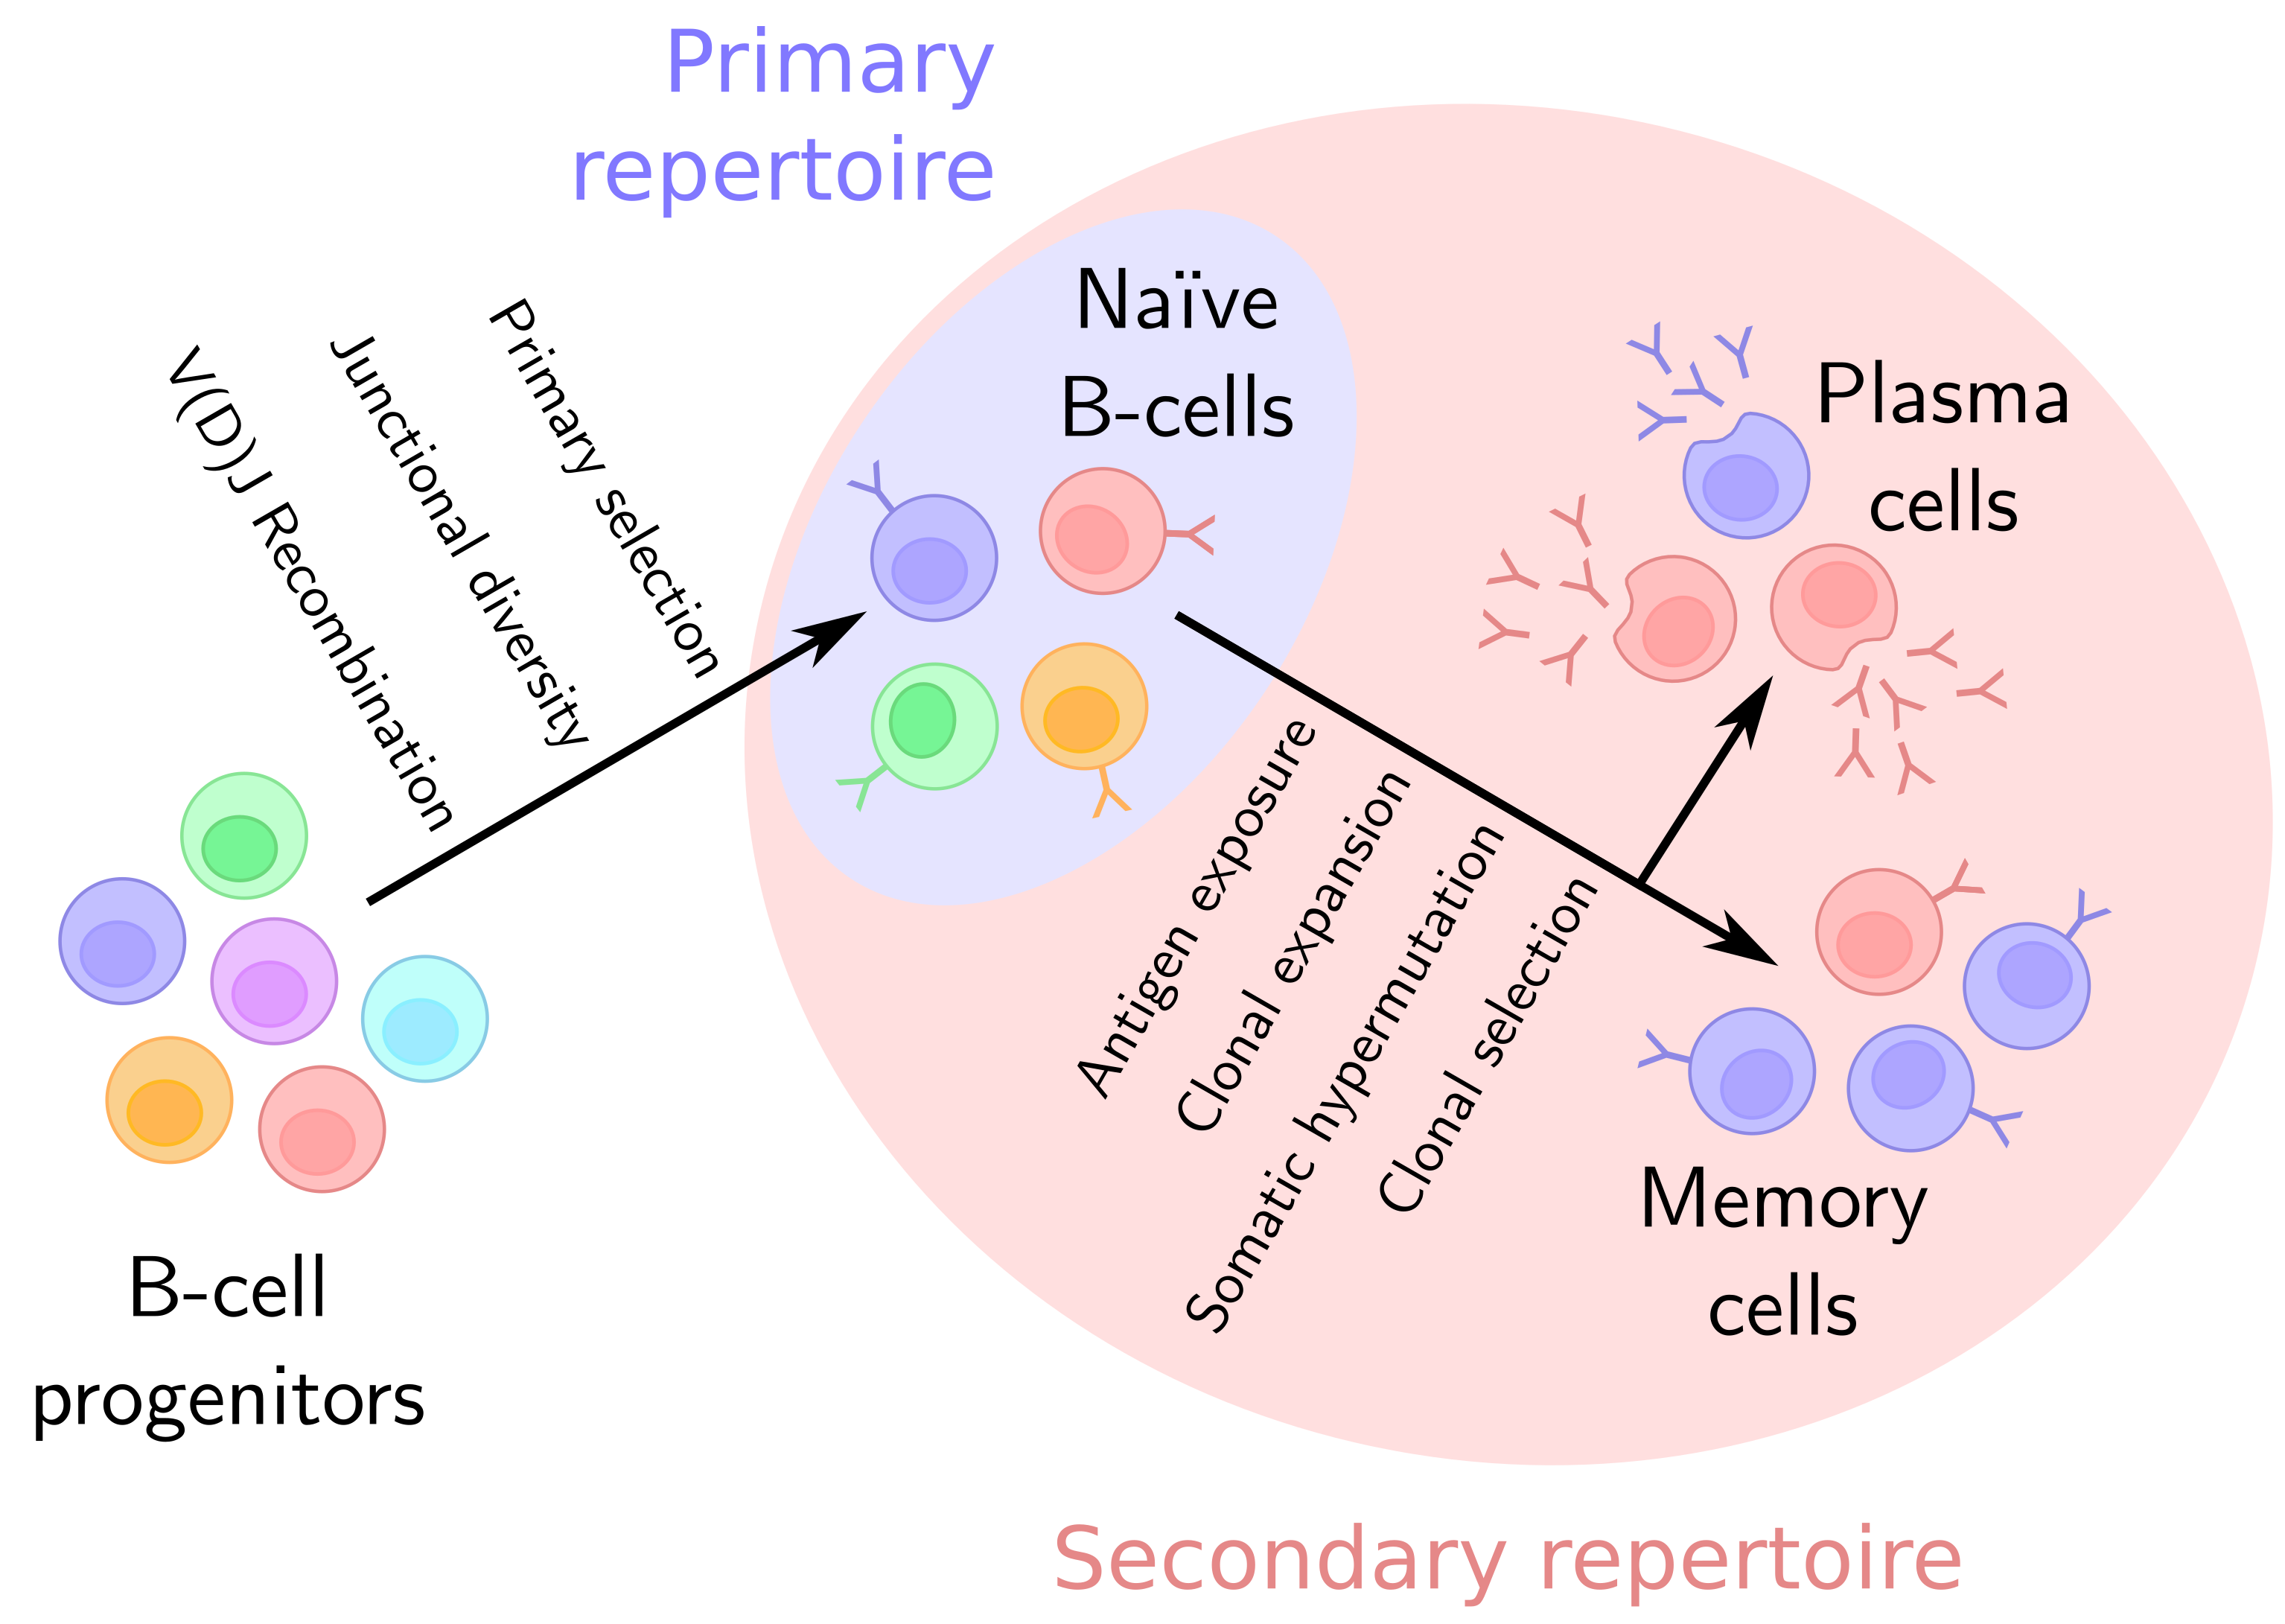
\includegraphics[width=0.9\textwidth]{_Figures/png_edited/bcell-repertoire-primary-secondary}
\caption{\textbf{Primary and secondary antibody repertoires:} Schematic of processes giving rise to the primary (\naive) and secondary (total) B-cell repertoires in the vertebrate immune system. Cell colours indicate clonal membership, with a loss of clonal diversity during primary development (left) and affinity maturation (right). Primary B-cell development (left) takes place in primary lymphoid organs (bone marrow in mammals, anterior kidney in teleosts), while affinity maturation (right) takes place in germinal centres (in mammals) or proto-germinal clusters (in teleosts) in secondary lymphoid organs such as the gut-associated lymphoid tissue (GALT) or spleen.}
\label{fig:intro-bcell-repertoires}
\end{figure}

\section{Humoral adaptive immunosenescence in vertebrates}
\label{sec:intro_immunosenescence}

The immune system of aged vertebrates has long been known to undergo a severe and systemic decline in functionality with age \parencite{segre1977immunosenescence}. As a result of this decline, older individuals exhibit increased susceptibility to a wide range of bacterial, viral, and fungal infectious diseases, as well as higher rates of complications and mortality from those infections when they occur \parencite{sambhara2009vaccination}. In addition, the effectiveness of vaccination against these infections often declines dramatically with age, with older individuals often receiving half or less of the immune protection from vaccination exhibited by younger recipients \parencite{sambhara2009vaccination}. Similar declines in immune functionality with age are also observed in other model organisms, and have been especially well-studied in mice, which share many details of their immune system with humans while being substantially easier to study in depth. While many different parts of the immune system are implicated in this immunosenescent phenotype \parencite{kogut2012bcells}, the decline in the humoral adaptive immune system has emerged as one particularly important contributor \parencite{ademokun2010ageing}.

The changes in the humoral immune system underlying its impaired functionality in old age begin at the level of B-cell development. In mice, the population of haematopoietic stem cells (HSCs) resident in the bone marrow increases in number but exhibits a decreased propensity to regenerate the pool of developing B-cells \parencite{ademokun2010ageing,kogut2012bcells}; factors contributing to this change include a deteriorating bone marrow niche, changes in blood-borne factors affecting HSC differentiation, and the well-known of older mammalian HSCs towards myeloid (rather than lymphoid) cell lineages \parencite{kogut2012bcells,dunnwalters2010bcellageing}. As a result of this change in HSC behaviour, the number of new B-cell progenitor and precursor cells in the bone marrow declines with age in mice; furthermore, these precursors exhibit decreased proliferation capacity, reduced rates of VDJ recombination and an increased rate of apoptosis \parencite{montecino2013immunosenescence,kogut2012bcells,labrie2004bone}. The rate of B-cell output from the bone marrow therefore declines significantly in aged mice compared to young adults, falling as low as 10\% of its level in young mice \parencite{kogut2012bcells}. As these \naive cells also have a shorter lifespan than antigen-experienced memory- and long-lived-plasma-cell populations, the net result of this decline in output from the bone marrow is a decrease in the number of \naive cells in the periphery and a progressive increase in the relative prevalence of antigen-experienced memory and plasma cells \parencite{mehr2011reversing,kogut2012bcells}; the pool of circulating immunoglobulins, meanwhile, becomes progressively dominated by hypermutated antibodies specific to previously-encountered antigens \parencite{kogut2012bcells}. As these \naive cells are essential for responding to novel or mutated immune threats not previously encountered by the immune system, this change is thought to lead to a progressive reduction in the capacity of the humoral immune system to respond effectively to novel threats \parencite{kogut2012bcells}.

Despite the decline in new \naive B-cells produced by the bone marrow, the total number of B-cells in aged mice does not appear to change significantly, reflecting an increase in the absolute number, as well as the relative prevalence, of antigen-experienced B-cell subpopulations. In humans, conversely, the absolute number of total B-cells appears to decline with age \parencite{ademokun2010ageing,montecino2013immunosenescence,aberle2013mechanistic}, with most B-cell subsets showing a significant decline in absolute abundance \parencite{frasca2011age}. Sources differ as to the age-related changes in relative abundance of different B-cell subtypes in humans, with some reporting an increase in the relative prevalence of \naive cells and decrease in that of memory cells\parencite{frasca2011age,blomberg2013age} and others reporting a more mouse-like shift in favour of the memory compartment \parencite{ademokun2010ageing}. These differences may arise from differences in the methods and cell markers used to quantify abundance of different B-cell populations \parencite{ademokun2010ageing}, genuine differences between populations, or the limitations of peripheral blood as a method of sampling the whole-body B-cell population of an individual \parencite{siegrist2009extremes}.

Whatever changes in cellular composition occur in ageing humans, it is clear that both humans and mice undergo a severe age-related decline in B-cell functionality. In humans, the best-understood aspect of this decline is a deterioration in the responsiveness of older patients to vaccination. Older humans frequently exhibit a substantially smaller \parencite{sambhara2009vaccination} and slower \parencite{kogut2012bcells} increase in the titre of antigen-specific serum antibodies in response to vaccination \parencite{sasaki2011limited,aberle2013mechanistic,ademokun2010ageing}, with defects in humoral response observed to vaccines for diseases as diverse as influenza, hepititis A and B, tetanus, diphtheria, pneumococcus and tick-borne encephalitis \parencite{dunnwalters2010bcellageing}. At least in the case of influenza, this decline in specific antibody production is primarily due to a decrease in the number of plasmablasts activated in response to vaccination \parencite{montecino2013immunosenescence,aberle2013mechanistic,sasaki2011limited}.

In addition to being less abundant, the antibodies produced by elderly humans in response to vaccination also appear to be of lower quality: anti-influenza antibodies produced by older human individuals demonstrate reduced ability to effectively neutralise viral haemagglutinin \parencite{kogut2012bcells,sasaki2011limited}, while IGHM antibodies produced by elderly subjects in response to pneumococcal polysaccharide vaccine demonstrate reduced opsonisation ability \parencite{kogut2012bcells}. While basal serum antibody titres actually increase rather than decrease with age in humans and mice \parencite{frasca2009ageing}, suggesting that antibody production \textit{per se} is not impaired with age, these antibodies also decline in quality \parencite{montecino2013immunosenescence}, with measurable increases in the rate of polyspecific and self-reactive antibodies produced in older individuals \parencite{kogut2012bcells}. This decline in baseline antibody quality in older individuals suggests a breakdown in primary B-cell selection in the bone marrow, enabling a greater number B-cells with low-specificity or self-reactive antibody sequences to emerge into the periphery \parencite{ademokun2010ageing}.

Various aspects of affinity maturation are also impaired in aged mammalian B-cells. While memory-cell clones established early in life often persist into old age, \naive B-cells in aged humans demonstrate a severely reduced ability to give rise to new antigen-specific memory B-cells following antigenic stimulation, impairing the establishment of functional immune memory for novel threats \parencite{aberle2013mechanistic}. B-cells from older humans and mice also exhibit impaired class-switch recombination capacity, possibly as a result of decreased AID expression \parencite{montecino2013immunosenescence,blomberg2013age,frasca2011age}, impairing the generation of antibodies with the same specificity but different effector functions. The decreased ability of older individuals to produce high-affinity antigen-specific antibodies \parencite{frasca2011age} also suggests a defect in affinity maturation, though this could also be attributable to the known ageing-related defects in the T-helper and follicular dendritic cells involved in secondary B-cell selection \parencite{montecino2013immunosenescence,aberle2013mechanistic,ademokun2010ageing} rather than changes in the B-cells themselves. Conversely, the effect of ageing on the somatic hypermutation process remains controversial \parencite{henry2019influenza,howard2006quality,ademokun2010ageing,frasca2009ageing}, with different groups reporting an increase, a decrease, or no change in the rate and level of SHM accumulation of different B-cell subtypes with age. 

The various cellular and population-level changes that occur in the humoral immune system with age naturally have important effects on the antibody repertoires of ageing individuals. Aged humans \parencite{siegrist2009extremes} and mice \parencite{dunnwalters2010bcellageing} exhibit increased rates of non-malignant clonal expansions in the memory-cell compartment, which when combined with the apparent maintenance or decline in total B-cell number would lead to a reduction in overall diversity \parencite{dunnwalters2010bcellageing}. Similarly, early techniques that investigated the repertoire by investigating the distribution of CDR3 lengths (CDR3 spetratyping) indicated that older humans frequently exhibit more distorted distributions dominated by CDR3 regions of a particular length, indicative of clonal expansion, and found that older individuals with more distorted spectratypes exhibited greater frailty and worse health and lifespan outcomes than those with more young-like spectratypes \parencite{gibson2009spectratyping}. On the basis of these and similar findings, the antibody repertoire has long been thought to decline in diversity in older individuals, impairing the adaptability of the ageing adaptive immune system.

More recently, the development of specialised high-throughput-sequencing-based techniques for interrogating antibody repertoires (\Igseq, or \igseq \parencite{weinstein2009igseq}) has enabled a few studies to investigate the ageing of these repertoires in greater detail. These studies, primarily on human peripheral blood, have confirmed many observations made using older lower-throughput methods: a reduced number of clonal lineages in older repertoires reflects decreased \naive-cell output from the bone marrow) \parencite{jiang2013vaccine}, while an increase in mean CDR3 length \parencite{wang2014ageing} and the average rate of premature STOP codons \parencite{debourcy2017ageing} in older repertoires similarly support the finding that primary and clonal selection are impaired with age. 
An increase in clonal expansion in older individuals is also observed: 
an \textit{oligoclonal} phenotype, in which one or a few large clones dominate the repertoire, is often seen in peripheral blood from elderly humans but very rarely in the young \parencite{wang2014ageing,debourcy2017ageing}. These expanded clones are persistent before and after vaccination \parencite{debourcy2017ageing} and even across multiple years \parencite{wang2014ageing}; in contrast, large clones observed in young human blood repertoires are typically transient responses to recent antigen challenge \parencite{wang2014ageing}.

The reduction in clonal richness and increase in clonal expansions seen in older individuals contribute to an overall reduction in the estimated number of unique sequences present in the peripheral repertoire \parencite{debourcy2017ageing}, a change observed for both \naive and mutated sequences and exacerbated by a significant reduction in within-clone sequence diversity in at least some elderly individuals \parencite{debourcy2017ageing}. The same study also found a drop in the percentage of unique sequences identified as coming from \naive B-cells, suggesting a mouse-like shift in repertoire prevalence towards antigen-experienced cell types \parencite{debourcy2017ageing}. However, while the alpha (within-individual) sequence diversity of the human peripheral repertoire appears to decline with age, the beta (between-individual) diversity of the repertoire actually increases, with repertoires from older individuals differing more from one another than those of young individuals \parencite{debourcy2017ageing}. Elderly repertoires also showed decreased flexibility in response to immune challenge, with repertoires taken from the same individual pre- and post-vaccination being significantly more similar in elderly than in young samples \parencite{debourcy2017ageing}, perhaps as a result of longer and more individualised histories of antigen exposure. Taken together, these findings suggest a pattern in which human peripheral antibody repertoires progressively lose diversity of the course of the human lifespan, while also becoming increasingly individualised and distinct.

In conclusion, there is strong evidence for a variety of developmental and physiological changes in the B-cell immune system with age in both mice and humans, giving rise to a severe decline in overall functional performance and immune protection. Many of these changes affect the composition of the antibody repertoire, with a reduction in clonal and sequence diversity and an increase in between-individual variability with age in human blood. However, despite this abundance of data, there remain some serious limitations in our knowledge of the ageing antibody repertoire.  From an evolutionary and comparative perspective, almost nothing is known about adaptive immunosenescence in species other than humans and mice; while several \igseq studies have been performed on teleost fish \parencite{weinstein2009igseq,jiang2011determinism,krasnov2017igseq,lund2019salmon,fu2018fugu}, for example, none to my knowledge have investigated B-cell immunosenescence in this taxon. Many of the findings reported above are specific to IGHG or IGHA antibodies in mice and humans \parencite{kogut2012bcells}, and may not generalise to species lacking these isotypes. Even in humans, the majority of immunosenescence studies, including virtually all repertoire studies, are limited to peripheral blood, and therefore primarily sample the minority of B-cells in transition between tissues; the majority of B-cells, which are resident in some immune organ or tissue, are systematically underrepresented in these samples \parencite{siegrist2009extremes,tabibiankeissar2016ageing}. Relatively little is therefore known about how the ageing of the B-cell repertoire differs between organs; the only paper I know of which investigated changes in antibody-repertoire diversity with age in biopsies from multiple human tissues failed to find any significant changes in alpha diversity, except for a significant \textit{increase} in repertoire sequence entropy in old spleen \parencite{tabibiankeissar2016ageing}. No published paper I know of has yet to investigate the ageing of the antibody repertoire at mucosal surfaces, where secreted antibodies play a particularly important role in regulating microbiotal communities and defending the body from pathogenic invasion.

In addition to this lack of spatial resolution in our knowledge of antibody repertoire ageing, there is a serious lack of temporal resolution; most studies of antibody repertoire ageing simply compare a ``young'' group (say 20-30 years of age) with one or two ``old'' groups (say $\geq70$ years of age), with little or no information about the intervening progression of any observed phenotypes \parencite{debourcy2017ageing,tabibiankeissar2016ageing}. The effect of known lifespan-increasing interventions on immune repertoire ageing also remains largely unstudied. Due to their very long lifespans and restrictions on experimental manipulation, humans are unsuitable subjects for these sorts of experiments, as are long-lived vertebrate model organisms such as zebrafish (median lifespan c. 3.5 years \parencite{gerhard2002zebrafish}) and \textit{Xenopus} (median lifespan c. 9 years \parencite{bowler1977longevity}). Even mice (median lifespan c. 2 to 2.5 years for the most common laboratory strains \parencite{yuan2009aging}), though widely used in biogerontology, are inconveniently long-lived for many ageing experiments. Conversely, many major model organisms in ageing research (such as fruit flies and nematode worms) are invertebrates, and so lack a mammal-like adaptive immune system. The development of a short-lived vertebrate species as a model organism for antibody-repertoire experiments would therefore be highly valuable for immunosenescence research, as well as ageing research more generally.

\section{The African turquoise killifish as a model for vertebrate ageing}
\label{sec:intro_killifish}

The genus \textit{Nothobranchius} comprises a broad group of annual freshwater fishes distributed across equatorial and subequatorial Africa \parencite{valdesalici2003lifespan}, with species diversity concentrated in the south-east of the continent \parencite{genade2005annual}. Members of this genus share a suite of adaptations to life in ephemeral pools and rivers, most notably the production of desiccation-resistant embryos capable of surviving through the dry season in a diapause state \parencite{genade2005annual}. Fish from this genus have been known for several decades to  exhibit very rapid growth and short lifespans, consistent with their evolving under conditions of very high extrinsic mortality \parencite{valdesalici2003lifespan}, with many species exhibiting a median lifespan of less than one year. Nevertheless, there is wide variation within the genus in body size, growth rate and lifespan, with species from less arid regions tending to show slower growth and longer median lifespans \parencite{genade2005annual}.

Like other \textit{Nothobranchius} species, the turquoise killifish (\nfu) is a medium-sized annual fish first isolated from ephemeral freshwater pools -- in this case, from a relatively arid region of southeastern Zimbabwe \parencite{genade2005annual,jubb1971new}. Even by the standards of the \textit{Nothobranchius} genus, \Nfu exhibits extremely rapid growth, maturation, and ageing, with the most widely-used laboratory strain (GRZ) exhibiting a median lifespan of just 9-16 weeks \parencite{valdesalici2003lifespan,genade2005annual,terzibasi2008strains,kirschner2012map,valenzano2015genome,smith2017microbiota} -- the shortest lifespan of any captive-bred vertebrate, and a dramatic outlier on the distribution of vertebrate lifespans. Combined with their possession of several important vertebrate-specific adaptations -- including an adaptive immune system -- this extremely short lifespan makes the turquoise killifish a highly promising model organism for ageing research \parencite{harel2015crispr}.

Despite its very short lifespan, \textit{N. furzeri} has been found to show a wide range of senescent phenotypes in even the shortest-lived strains, including lipofuscin deposition \parencite{genade2005annual};  accumulation of senescence markers \parencite{genade2005annual};  increased neurodegenaration \parencite{valenzano2006resveratrol1,valenzano2006resveratrol2}; impaired learning and behavioural phenotypes  \parencite{genade2005annual,valenzano2006resveratrol1}; and a high incidence of degenerative and neoplastic lesions \parencite{dicicco2011histopathology}. These diverse phenotypes indicate that the short lifespan of the turquoise killifish is the result of an accelerated general ageing process, rather than the specific failure of a particular organ or system. Moreover, established anti-ageing interventions such as resveratrol treatment \parencite{valenzano2006resveratrol1}, reduction in ambient temperature \parencite{valenzano2006temperature} and dietary restriction \parencite{terzibasi2009dr} also extend lifespan in the turquoise killifish, indicating a strong analogy with the ageing phenotypes observed in canonical model systems.

Due primarily to its potential as a model organism for ageing research, the turquoise killifish has also seen rapid development as a genetic model. The short-lived GRZ strain has been bred in captivity for fifty years and at least a hundred generations \parencite{terzibasi2007review} and exibits a very high degree of homozygosity \parencite{kirschner2012map,reichwald2009genome,valenzano2009map}, providing a uniform genetic background for experimental interventions. A number of important genetic resources are now available, including several assemblies of the nuclear genome \parencite{reichwald2015genome,valenzano2015genome,willemsen2019popgen}, the most recent of which (\parencite{willemsen2019popgen}, in preparation) is of very high quality. These assemblies have yielded a genome with an estimated size of roughly 1.5 gigabases \parencite{willemsen2019popgen};
karyotyping \parencite{reichwald2009genome} and sequencing analysis \parencite{reichwald2015genome} both indicate a chromosome number of $2n = 38$, corresponding to 19 distinct linkage groups in the haploid genome.

Prior to the work contained in this thesis, almost nothing was known about the adaptive immune system of the turquoise killifish. However, as a teleost, and therefore as a jawed vertebrate, it could be strongly expected to have a roughly mammal-like adaptive immune system, and a number of genes related to B-cell adaptive immunity (including \gene{RAG1}, various B-cell developmental markers, and fragments of antibody genes) were identified in one or more genome annotations. Phylogenetically, the genus \textit{Nothobranchius} falls within the Cyprinodontiformes, and the turquoise killifish is therefore relatively closely related to several species with previously-characterised \igh{} loci, including fugu, stickleback and medaka \parencite{terzibasi2007review,hughes2018teleostphylo}. Despite the relatively unknown state of adaptive immunity in the turquoise killifish, therefore, there was good reason to believe it possessed a functional B-cell immune system similar to those of other teleosts, and therefore comparable in many respects with those of mammalian species, including humans. When combined with its short lifespan and rapid ageing phenotype, this makes the turquoise killifish a potentially highly-valuable model for studying the forms and mechanisms of humoral adaptive immunosenescence in jawed vertebrates. In this thesis, therefore, I characterised the \igh{} locus of the turquoise killifish, established a working \igseq protocol, and performed the first experiments investigating adaptive immunosenescence in this species.

\begin{figure}
\centering
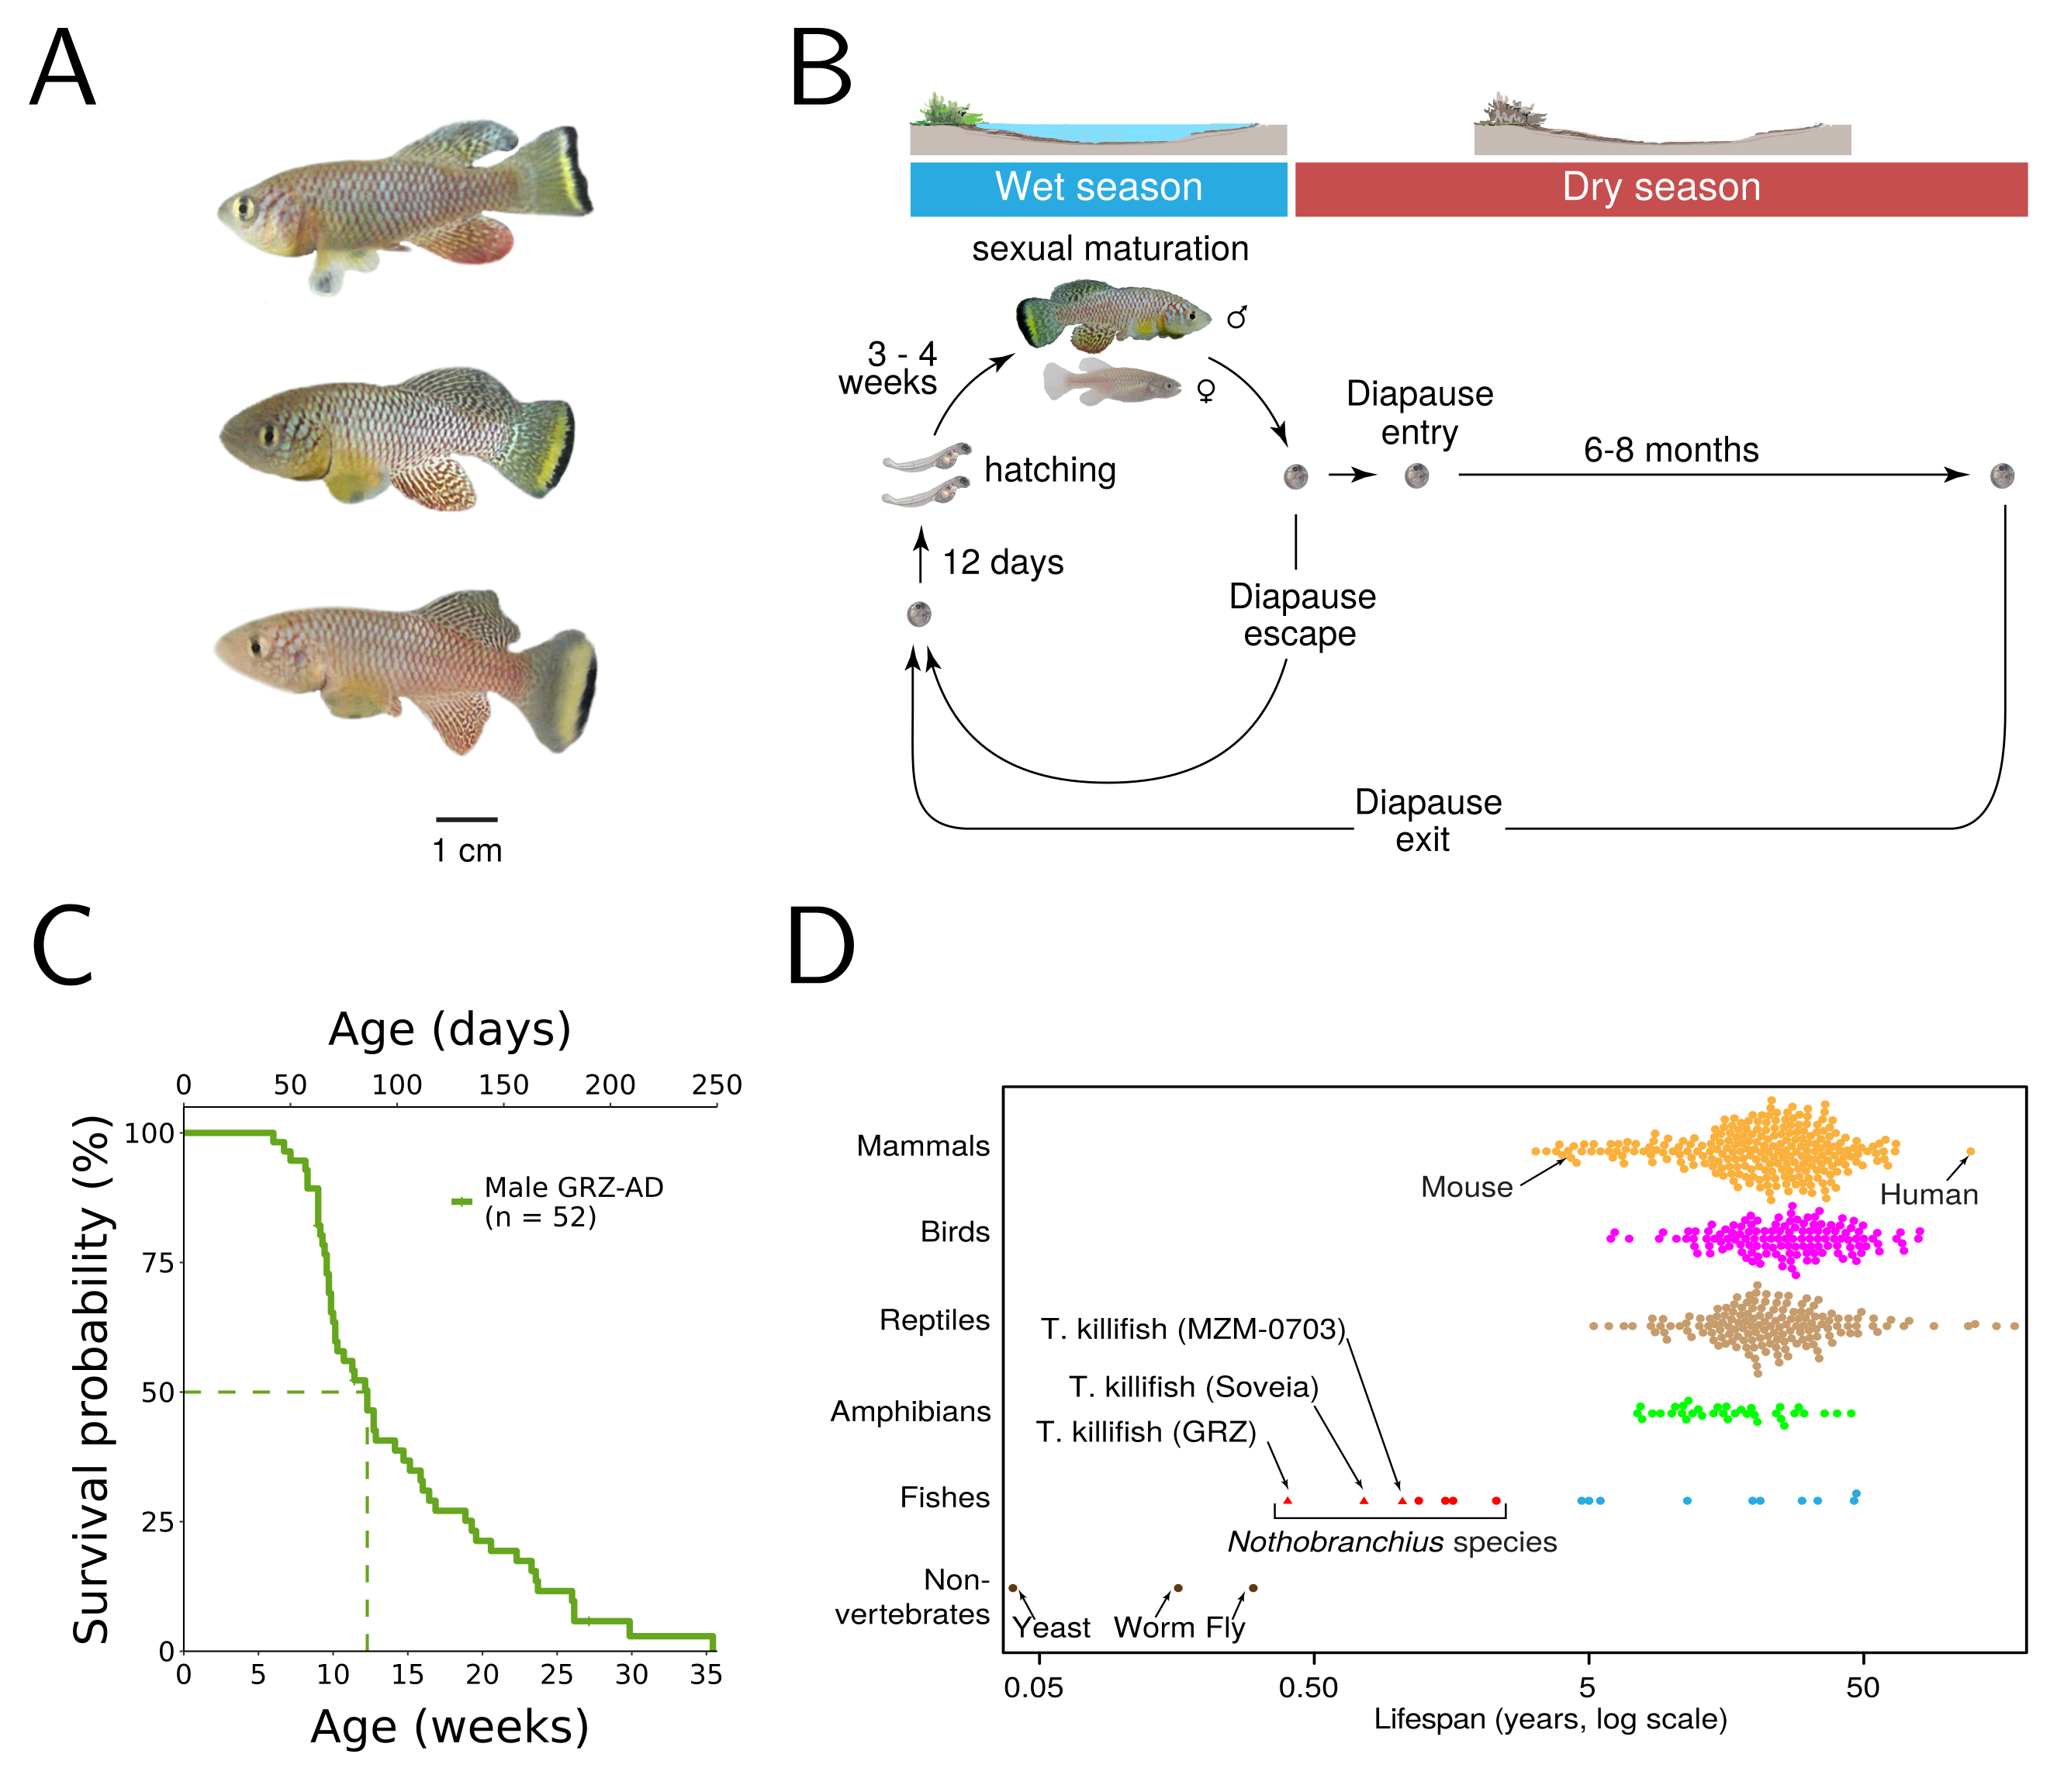
\includegraphics[width=0.95\textwidth]{_Figures/png_edited/intro-turquoise-killifish}
\caption[The turquoise killifish (\nfu) as a model for vertebrate ageing]{\textbf{The turquoise killifish (\nfu) as a model for vertebrate ageing:} (A) Photographs of adult male yellow-tailed turquoise killifish.
(B) Life cycle of the turquoise killifish in its natural environment, showing hatching and breeding during the rainy season and embryo survival in diapause during the dry season.
(C) Example lifespan curve of short-lived GRZ-AD turquoise-killifish males, hatched in December 2016, with a median lifespan of roughly 12 weeks.
(D) Comparison of turquoise-killifish maximum lifespan (red triangles) to other vertebrate species, demonstrating the extremely short lifespan of \Nfu compared to other vertebrates. (A), (B) and (D) adapted from \parencite{valenzano2015genome}, Figure 1.}
\end{figure}
%!TEX root = ../thesis.tex
% TODO: Change this?

\chapter{Materials and methods}  
\onehalfspacing

\pagebreak

%%%%%%%%%%%%%%%%%%%%%%%%%%%%%%%%%%%%%%%%%%%%%%%%%%%%%%%%%%%%%%%%%%%%%%%%%%%%%%%
% FISH HUSBANDRY SECTION
%%%%%%%%%%%%%%%%%%%%%%%%%%%%%%%%%%%%%%%%%%%%%%%%%%%%%%%%%%%%%%%%%%%%%%%%%%%%%%%

\section{Killifish husbandry and sample preparation methods}
\label{sec:methods_husbandry}

Male turquoise killifish (\nfu, GRZ-AD strain) from a single hatching were raised under standard husbandry conditions \parencite{dodzian2018husbandry} and housed from four weeks post-hatching in individual \lt{2.8} tanks connected to a water recirculation system. Fish received \hr{12} of light per day on a regular light/dark cycle, and were fed blood
worm larvae and brine shrimp nauplii twice a day during the week and once a day during the weekend \parencite{dodzian2018husbandry,smith2017microbiota}.

Sacrificed fish (\Cref{tab:igseq-cohorts-fish}) were killed by anaesthetisation in \gl{1.5} Tricaine solution in room-temperature tank water \parencite{carter2011tricaine}, then flash-frozen in liquid nitrogen and ground to a homogenous powder with a pestle in a liquid-nitrogen-filled mortar. The powder was mixed thoroughly and stored at \degC{-80} prior to RNA isolation.

%%%%%%%%%%%%%%%%%%%%%%%%%%%%%%%%%%%%%%%%%%%%%%%%%%%%%%%%%%%%%%%%%%%%%%%%%%%%%%%
% MOLECULAR/WETLAB SECTION
%%%%%%%%%%%%%%%%%%%%%%%%%%%%%%%%%%%%%%%%%%%%%%%%%%%%%%%%%%%%%%%%%%%%%%%%%%%%%%%

\section{Biochemistry and molecular biology methods}

\subsection{Standard methods}

\subsubsection{PCR}
\label{sec:methods_molec_standard_pcr}

The polymerase chain reaction is a well-established method for rapid amplification of a DNA sequence through repeated cycles of denaturation, priming and replication by a high-temperature-tolerant DNA polymerase enzyme \parencite{paul2010hotstartpcr}. Unless otherwise specified, all PCRs in this chapter were performed using \x{2} Kapa HiFi HotStart ReadyMix PCR Kit (\Cref{app:solutions_enzymes}) according to the manufacturer's instructions. Briefly, for a \ul{25} reaction, \ul{12.5} Kapa ReadyMix was combined with \ul{12.5} total of template, nuclease-free water, and primers; these volumes were scaled linearly for reactions of different volumes. The mixture was then heated in a thermocycler as follows:

\begin{center}
\begin{threeparttable}
\begin{tabular}{cccc}\toprule
\textbf{Step} & \textbf{Temperature [\degC{}]} & \textbf{Duration [\secs{}]} & \textbf{Cycles}\\\midrule
Initial denaturation & 95 & 180 & 1 \\\midrule
Denaturation & 98 & 20 & \multirow{3}{*}{$n_c$\tnote{a}}\\
Annealing & $T_a$\tnote{a} \tnote{} & 15 & \\
Extension & 72 & $t_{ext}$\tnote{a} & \\\midrule
Final extension & 72 & $t_{ext} \times 4$\tnote{a} & 1\\
\bottomrule\end{tabular}
\begin{tablenotes}
\item[a] Annealing temperature ($T_a$), extension time ($t_{ext}$) and cycle number ($n_c$) determined separately for each reaction.
\end{tablenotes}
\end{threeparttable}
\end{center}

\subsubsection{Nucleic-acid purification with SeraSure magnetic beads}
\label{sec:methods_molec_standard_serasure}

Nucleic-acid isolation, size-selection and concentration in the \igseq library preparation protocol (and elsewhere where necessary) was performed using SeraSure SPRI (solid phase reversible immobilization) bead preparations \parencite{hawkins1994spri,deangelis1995spri,lennon2010cleanup,fisher2011cleanup}. In SPRI, paramagnetic beads bind DNA in the presence of polyethylene glycol (PEG), with the affinity of the beads for DNA depending on the concentration of PEG in the binding buffer. As a result, the range of nucleic-acid sequence lengths retained by SPRI bead purification depends primarily on the concentration of PEG, which in turn depends on the relative volume of SeraSure bead suspension added to a sample; the higher the concentration, the shorter the minimum fragment length retained during the purification process. In combination with a magnetic rack to remove the DNA-bound beads from suspension, this allows DNA of the desired size range to be isolated from a solution and resuspended in the desired volume of fresh buffer.

To prepare \ml{50} of SeraSure bead suspension for DNA (or DNA:RNA heteroduplex) isolation, a stock of SeraMag beads (\Cref{app:solutions_reagents}) was vortexed thoroughly, then \ml{1} was transferred to a new tube. This tube was then transferred to a magnetic rack and incubated at room temperature for \mins{1}, then the supernatant was removed and replaced with \ml{1} TET buffer (\Cref{app:solutions_buffers}) and the tube was removed from the rack and vortexed thoroughly. This washing process was repeated twice more, for a total of three washes in TET. A fourth cycle was used to replace the TET with incomplete SeraBind buffer (iSB, \Cref{app:solutions_buffers}). The vortexed \ml{1} aliquot of beads in iSB was then transferred to a conical tube containing \ml{28} iSB and mixed by inversion. To add the PEG, \ml{20} \pc{50} (w/v) PEG 8000 solution was dispensed slowly down the side of the conical tube, bringing the total volume to \ml{49}. Finally, this was brought to \ml{50} by adding \ul{250} \pc{10} (w/v) Tween 20 solution and \ul{750} autoclaved water to complete the SeraSure bead suspension.

To perform a bead cleanup, an aliquot of prepared SeraBind solution was vortexed thoroughly to completely resuspend the beads, then the appropriate relative volume of SeraSure suspension was added to a sample, mixing thoroughly by gentle pipetting. The sample was incubated at room temperature for \mins{5} to allow the beads to bind the DNA, then transferred to a magnetic rack and incubated for a further \mins{5} to draw as many beads as possible out of suspension. The supernatant was removed and discarded and replaced with \pc{80} ethanol, to a volume sufficient to completely submerge the bead pellet. The sample was incubated for 0.5-\mins{1}, then the ethanol was replaced and incubated for a further 0.5-\mins{1}. The second ethanol wash was removed, and the tube left on the rack until the bead pellet was almost, but not completely, dry, after which it was removed from the rack. The bead pellet was resuspended in a suitable volume of elution buffer (EB, \Cref{app:solutions_buffers}) then incubated at room temperature for at least 5 minutes to allow the nucleic-acid molecules to elute from the beads.

Unless otherwise specified, the beads from a cleanup were left in a sample during subsequent applications. To remove beads from a sample, the sample was mixed gently but thoroughly to resuspend the beads, incubated for an extended time period (at least \mins{10}) to maximise nucleic-acid elution, then transferred to a magnetic rack and incubated for 2-\mins{5} to remove the beads from suspension. The supernatant (containing the eluted nucleic-acid molecules) was then transferred to a new tube, and the beads discarded.

\subsubsection{Phenol-chloroform extraction and ethanol precipitation of DNA}
\label{sec:methods_molec_standard_phenol}

% TODO: Explain and cite phenol-chloroform extraction

To remove RNA and protein from isolated DNA samples, each sample was diluted to \ul{500} in nuclease-free water and mixed with \ul{500} of equilibrated phenol:chloroform:isoamyl alcohol (PCI) mixture (\Cref{app:solutions_reagents}) in a fume hood. The sample/PCI mixture was shaken vigorously by had for \secs{15} to thoroughly mix the different components, then centrifuged in a benchtop centrifuge (\mins{5}, room temperature, top speed). Again in a fume hood, the mixed sample was angled at \degrees{45}, and the upper aqueous phase containing the DNA was removed and transferred to a new tube while the lower organic phase was discarded. A second aliquot of \ul{500} PCI was added and the sample was mixed, centrifuged and separated as before. Finally, in order to remove residual phenol in the sample, \ul{500} pure chloroform was added to the newly-separated aqueous phase and the sample was once again mixed, centrifuged and separated. 

% TODO: Citation for ethanol precipitation

Following this final round of separation, the DNA in the aqueous phase was precipitated by addition of 0.1 volumes of \mol{3} sodium acetate solution, followed by 2.5 volumes of fresh \pc{100} ethanol. The mixture was mixed gently by inversion, then incubated for 1-\hr{3} at \degC{-80} or at \degC{-20} overnight. The suspension of precipitated DNA was pelleted through centrifugation in a benchtop centrifuge (\mins{30}, \degC{4}, top speed). The supernatant was discarded and replaced with \ul{500} chilled \pc{70} ethanol, and the sample centrifuged again (\mins{5}, \degC{4}, top speed). After this, the supernatant was again discarded, and the samples allowed to air-dry before being resuspended in 30-\ul{50} EB (\Cref{app:solutions_buffers}). 

\subsubsection{Guanidinium thiocyanate-phenol-chloroform extraction of RNA}
\label{sec:methods_molec_standard_qiazol}

% TODO: Explain and cite TRIzol isolation

To isolate total RNA from homogenised killifish tissues, \ml{1} of QIAzol lysis reagent (\Cref{app:solutions_reagents}, containing acid phenol and guanidinium thiocyanate) was added to \g{0.1} of tissue, mixed gently but thoroughly by inversion, then incubated at room temperature for \mins{5} to allow the QIAzol to penetrate the tissue. 0.2 volumes of chloroform was added and the mixture was shaken vigorously for \secs{15}, then incubated at room temperature for \mins{3}. The mixture was then centrifuged (\mins{15}, \degC{4}, \g{12000}). Angling the tube at \degrees{45}, the upper aqueous phase containing the RNA was removed and transferred to a new tube, while the lower organic phase was discarded.

Following phase separation, the RNA was precipitated by adding 0.5 volumes of room-temperature isopropanol, mixing gently by inversion and incubating for \mins{5} at room temperature. The suspension was centrifuged (\mins{10}, \degC{4}, \g{12000}) and the supernatant discarded. 1 volume of freshly prepared \pc{75} ethanol was added and the tube was vortexed briefly and centrifuged again (\mins{5}, \degC{4}, \g{7500}). The supernatant was discarded and the RNA pellet allowed to air-dry for 5-\mins{10}, then resuspended in \ul{50} EB (\Cref{app:solutions_buffers}). The concentration and quality of the resulting total-RNA solution were assayed with the Qubit 2.0 flourometer (Thermo Fisher, RNA BR assay kit) and TapeStation 4200 (Agilent, RNA tape), respectively, according to the manufacturer's instructions.

\subsection{Library size-selection with the BluePippin}
\label{sec:methods_molec_standard_bluepippin}

The BluePippin (Sage Science) is a DNA size-selection system based on agarose gel electrophoresis, which uses timed switching between positively-charged electrodes at a forked gel channel in an agarose cassette to redirect DNA of a desired size range into a separate lane from the rest of the sample \parencite{sage2016bluepippin}. The timing of switching is determined based on the size range input by the user and calibrated using flourescent internal standards, which are added to the sample during the sample preparation process and designed to run well ahead of the possible size ranges for that cassette type. The combination of the choice of cassette and the choice of standards determines which fragment lengths can be effectively isolated using the machine.

For the experiments described in this thesis, a \pc{1.5} cassette with R2 markers were used, enabling size selection of targets in the range of 250--\bp{1500} \parencite{sage2016bluepippin}. Machine calibration and testing, cassette preparation, and protocol design were performed in accordance with the BluePippin documentation and instructions given by the machine software. During this process, the elution wells of the lanes to be used in the size-selection run were emptied and refilled with \ul{40} of electrophoresis buffer (\Cref{app:solutions_reagents}), then sealed for the duration of the run, and a broad-range size-selection protocol with a target range of 400 to \bp{800} was specified. \ul{30} of sample was then combined with \ul{10} of loading solution (\Cref{app:solutions_reagents}) and vortexed to mix, then \ul{40} of buffer was removed from the appropriate loading well and replaced, slowly, with the prepared sample mixture. The protocol was started and run until the final elution was complete. Finally, the eluted samples were removed from the elution wells of the appropriate lanes, and the unused lanes of the cassette were re-sealed for future use.

\subsection{BAC isolation and sequencing}
\label{sec:methods_molec_bacs}

All BAC clones that were sequenced for this research were provided by the FLI in Jena as plate or stab cultures of transformed \textit{E. coli}, which were replated and stored at \degC{4} when not in use. Prior to isolation, the clones of interest were cultured overnight in at least \ml{100} LB medium to produce a large liquid culture. The cultures were then transferred to \ml{50} conical tubes and centrifuged (10-\mins{25}, \degC{4}, \g{3500}) to pellet the cells. After pelleting, the supernatant was carefully discarded and the cells were resuspended in \ml{18} buffer P1 (\Cref{app:solutions_buffers}).

% TODO: Reference (/explanation?) for alkaline lysis

After resuspension, the cultures underwent alkaline lysis to release the BAC DNA and precipitate genomic DNA and cellular debris. \ml{18} lysis buffer P2 (\Cref{app:solutions_buffers}) was added to each tube, which was then mixed gently but thoroughly by inversion and incubated at room temperature for \mins{5}. \ml{10} ice-chilled neutralisation buffer P3 (\Cref{app:solutions_buffers}) was added and each tube was mixed gently but thoroughly by inversion and incubated on ice for \mins{15}. The tubes were then centrifuged (20-\mins{30}, \degC{4}, \g{12000}) to pellet cellular debris and the supernatant transferred to new conical tubes. This process was repeated at least two more times, until no more debris was visible in any tube; this repeated pelleting was necessary to minimise contamination in each sample, as the normal column- or paper-based filtering steps used during alkaline lysis protocols result in the loss of the BAC DNA.

Following alkaline lysis, the BAC (and residual genomic) DNA in each sample underwent isopropanol precipitation: 0.6 volumes of room-temperature isopropanol was added to the clean supernatant in each tube, followed by 0.1 volumes of \mol{3} sodium acetate solution. Each tube was mixed well by inversion, incubated for 10-\mins{15} at room temperature, then centrifuged (\mins{30}, \degC{4}, \g{12000}) to pellet the DNA. The supernatant was discarded and the resulting DNA smear was ``resuspended'' in \ml{1} \pc{100} ethanol and transferred to a \ml{1.5} tube, which was re-centrifuged (\mins{5}, \degC{4}, top speed) to obtain a concentrated pellet. Finally, the peletted samples were resuspended in EB (\Cref{app:solutions_buffers}) and purified of proteins and RNA using phenol:chloroform extraction and ethanol precipitation (\Cref{sec:methods_molec_standard_phenol}).

The resuspended BAC isolates were sent to the Cologne Center for Genomics, where they underwent Illumina Nextera XT library preparation and were sequenced on an Illumina MiSeq sequencing machine (MiSeq Reagent Kit v3, 2x300bp reads).

\subsection{Immunoglobulin sequencing of killifish samples}
\label{sec:methods_molec_igseq}

\subsubsection{RNA template quantification and quality control}
\label{sec:methods_molec_igseq_template}

Total RNA from whole-body killifish samples was isolated as described in \Cref{sec:methods_molec_standard_qiazol}; gut RNA from microbiota transfer experiments \parencite{smith2017microbiota} was already prepared and available. Quantification of RNA samples was performed with the Qubit 2.0 flourometer (RNA BR assay kit), while quality control and integrity measurement was performed using the TapeStation 4200 (RNA tape), both according to the manufacturer's instructions.

\subsubsection{Reverse-transcription and template switching}
\label{sec:methods_molec_igseq_rt}

Reverse transcription of total RNA and template switching for \igseq library preparation was performed using SMARTScribe Reverse Transcriptase (\Cref{app:solutions_enzymes}), in line with the protocol specified in \parencite{turchaninova2016igprep} (Procedure, steps 5-9). Briefly, \ng{750} total RNA from a killifish sample was combined with \ul{2} \umol{10} gene-specific primer (GSP), homologous with the second \ch exon of \Nfu \igh{M} (\Cref{app:oligos_primers}, designed using \program{Primer3} \parencite{untergasser2012primer3}). The reaction volume was brought to a total of \ul{8} with nuclease-free water, and the resulting mixture was incubated for 2 minutes at \degC{70} to denature the RNA, then cooled to \degC{42} to anneal the GSP. % TODO: Citation for purpose of incubation steps (Vollmers?)

Following annealing, the RNA-primer mixture was combined with \ul{12} of reverse-transcription master-mix (\Cref{tab:methods_rt_mm}), including the reverse-transcriptase enzyme and template-switch adapter (\Cref{app:oligos_tsa}, sequence provided in \parencite{turchaninova2016igprep}). The complete reaction mixture was incubated at for \hr{1} at \degC{42} for the reverse-transcription reaction, then mixed with \ul{1} of uracil DNA glycosylase (UDG, \Cref{app:solutions_enzymes}) and incubated for a further \mins{40} at \degC{37} to digest the template-switch adapter. Finally, the reaction product was purified using SeraSure beads (\Cref{sec:methods_molec_standard_serasure}) at \x{0.7} concentration, eluting in \ul{16.5} clean elution buffer (EB, \Cref{app:solutions_buffers}).

\begin{table}[h]
\begin{center}\small
\begin{threeparttable}
\caption{Master-mix components for SMARTScribe reverse transcription, per sample}
\begin{tabular}{llll}\toprule
\textbf{Volume [\ul{}]} & \textbf{Component} & \textbf{Concentration} & \textbf{Reference}\\\midrule
2 & SMARTScribe reverse transcriptase & \unitsul{100} & \Cref{app:solutions_enzymes} \\
4 & SMARTScribe first-strand buffer & \x{5} & \Cref{app:solutions_reagents} \\
2 & SmartNNNa barcoded TSA & \umol{10} & \Cref{app:oligos_tsa}\\
2 & DTT & \mmol{20} & \Cref{app:solutions_reagents}\\
2 & dNTP mix & \umol{10} per nucleotide & \Cref{app:solutions_reagents}\\
0.5 & RNasin RNase inhibitor & \unitsul{40} & \Cref{app:solutions_enzymes}\\\bottomrule
\end{tabular}
\label{tab:methods_rt_mm}
\end{threeparttable}
\end{center}
\end{table}

\subsubsection{PCR amplification and adapter addition} 
\label{sec:methods_molec_igseq_pcr}

Following reverse-transcription, UDG digestion, and cleanup, the reaction mixture underwent three successive rounds of Kapa PCR (\Cref{sec:methods_molec_standard_pcr}, \Cref{tab:methods_igseq_pcr}) each of which was followed by a further round of bead cleanups (\Cref{sec:methods_molec_standard_serasure}, \Cref{tab:methods_igseq_beads}). The first of these PCR reactions added a second strand to the reverse-transcribed cDNA and amplified the resulting DNA molecules; the second added partial Illumina sequencing adapters and further amplified the library, and the third added complete Illumina adapters (\Cref{app:oligos_illumina}, including i5 and i7 indices \parencite{illumina2018adapters}). Primer sequences (\Cref{app:oligos_primers}) homologous to the template-switch adapter (M1SS and M1S) were provided by \parencite{turchaninova2016igprep}, while those homologous to the \cm{1} constant-region exon (IGHC-B and IGHC-C) were designed using \program{Primer3} \parencite{untergasser2012primer3}.

\begin{table}[h]
\def\arraystretch{1.3}
\centering\small
\begin{threeparttable}
\caption{Details of PCR protocols for \Nfu immunoglobulin sequencing}
\begin{tabular}{c|ccc|cc|ccccc}\toprule
\multirow{2}{*}{\textbf{PCR}} & \multicolumn{3}{c|}{\textbf{Protocol details}} & \multicolumn{2}{c|}{\textbf{Primers}} & \multicolumn{4}{c}{\textbf{Volumes (\ul{})\tnote{b}}}\\
 & \# cycles & $T_m$ (\degC{}) & $t_\mathrm{ext}$ (\secs{}) & F & R & Template & Primers (each) & Kapa & H\textsubscript{2}O \\\midrule
1 & 18 & 65 & 15 & IGHC-B & M1SS & 10.5 & 1 (\x{}2) & 12.5 & 0 \\\midrule
2 & 13 & 65 & 15 & M1S+P2 & IGHC-C+P1 & 1 & 0.5 (\x{}2) & 12.5 & 10.5 \\\midrule
3 & 7 to 12\tnote{c} & \textbf{68} & 15 & D50*\tnote{a} & D7**\tnote{a} & 2 & \textbf{0.75} (\x{}2) & 12.5 & 9 \\
\bottomrule
\end{tabular}
\begin{tablenotes}
\item[a] PCR3 primers selected as appropriate for each library's assigned indices; see \Cref{app:oligos_illumina} for more information.
\item[b] If the number of samples to be sequenced was small, all volumes of PCR 3 were doubled for a \ul{50} total PCR volume.
\item[c] See \Cref{tab:methods_igseq_cycles} for specific cycle numbers used in each experiment.
\end{tablenotes}
\label{tab:methods_igseq_pcr}
\end{threeparttable}
\end{table}

\begin{table}[h]
\def\arraystretch{1.5}
\centering\small
\caption{Details of bead cleanups during \Nfu immunoglobulin sequencing}
\begin{threeparttable}
\begin{tabular}{l|c|cc|c}\toprule
\multirow{2}{*}{\textbf{Stage}\tnote{a}} & \multirow{2}{*}{\textbf{Sample volume}} & \multicolumn{2}{c|}{\textbf{Beads volume (\ul{})}} & \multirow{2}{*}{\textbf{Elution volume (\ul{})}\tnote{c}}\\
& & \ul{} & \x{}\tnote{b} & \\\midrule
RT & 21 & 14.7 & 0.7 & 16.5\\
PCR 1 & 25 & 17.5 & 0.7 & 25\\
PCR 2 & 25 & 17.5 & 0.7 & 15\\
PCR 3 & 25\tnote{d} & 20\tnote{d} & 0.8 & 15\tnote{d}\\
Pooling & Varies\tnote{e} & Varies\tnote{e} & 2.5 & 35\\ 
\bottomrule
\end{tabular}
\begin{tablenotes}
\item[a] Each bead cleanup takes place immediately \textit{after} its corresponding stage.
\item[b] Bead volumes are usually given as multiples of the sample volume.
\item[c] All elutions performed in the specified volume of elution buffer (EB, \Cref{app:solutions_buffers}).
\item[d] If PCR 3 reaction volume differs from \ul{25}, bead and elution volumes are rescaled proportionally to sample volume as appropriate.
\item[e] Samples are pooled in equimolar ratio.
\end{tablenotes}
\label{tab:methods_igseq_beads}
\end{threeparttable}
\end{table}

\begin{table}[h]
\def\arraystretch{1.3}
\centering\small
\caption{PCR cycle numbers used for \Nfu immunoglobulin sequencing}
\begin{threeparttable}
\begin{tabular}{c|ccc|cc|ccccc}\toprule
\multirow{2}{*}{\textbf{Experiment}} & \multicolumn{3}{c|}{\textbf{Number of PCR cycles}} & \multirow{2}{*}{\textbf{Reference}}\\
& PCR 1 & PCR 2 & PCR 3 &\\\midrule
Pilot & 18 & 13 & 9 & \Cref{sec:igseq_pilot}\\
Ageing & 18 & 13 & 8 & \Cref{sec:igseq_ageing}\\
Gut & 18 & 13 & 12 &\Cref{sec:igseq_gut}\\
\bottomrule
\end{tabular}
\label{tab:methods_igseq_cycles}
\end{threeparttable}
\end{table}

\subsubsection{Library pooling, size selection and sequencing} 
\label{sec:methods_molec_igseq_seq}

Following PCR3 and its attendant bead cleanup, the total concentration of each library was assayed with the Qubit 2.0 (DNA HS assay kit), while the size distribution of each library was obtained using the TapeStation 4200 (D1000 tape). To obtain the concentration of complete library molecules in each case (as opposed to primer dimers or other off-target bands), the ratio between the concentration of the desired library band (c. 620-\bp{680}) and the total concentration of the sample in the TapeStation assay was calculated for each TapeStation lane, and the total concentration of each library as measured by the Qubit was multiplied by this number to obtain an estimate of the desired figure:

\begin{equation}
\mathrm{Library~concentration} (L) = \mathrm{Qubit~concentration} \times \frac{\mathrm{TapeStation~concentration~[main~band]}}{\mathrm{TapeStation~concentration~[total]}}
\label{eq:library-conc}
\end{equation}

\noindent All the libraries for a given experiment were then pooled, such that the estimated concentration $L$ of each library in the final pooled sample was equal and the total mass of nucleic acid in the pooled sample was at least \ng{240}. The pooled libraries underwent a final bead cleanup (\Cref{sec:methods_molec_standard_serasure}, \Cref{tab:methods_igseq_beads}) to concentrate the samples, then underwent size selection with the BluePippin (\Cref{sec:methods_molec_standard_bluepippin}, \pc{1.5} DF Marker R2, broad 400-800bp). The size-selected pooled samples underwent a final round of quality control (as above) to confirm their collective concentration (at least \nmol{1.5}) and size distribution (one peak at c. 620-\bp{680}). Finally, the pooled and size-selected libraries were sequenced externally on an Illumina MiSeq System (MiSeq Reagent Kit v3, 2x300bp reads, 30\% PhiX spike-in), either at the Cologne Center for Genomics (pilot and ageing experiments) or with Admera Health (gut experiment).

%%%%%%%%%%%%%%%%%%%%%%%%%%%%%%%%%%%%%%%%%%%%%%%%%%%%%%%%%%%%%%%%%%%%%%%%%%%%%%%
% COMPUTATIONAL/BIOINFORMATIC SECTION
%%%%%%%%%%%%%%%%%%%%%%%%%%%%%%%%%%%%%%%%%%%%%%%%%%%%%%%%%%%%%%%%%%%%%%%%%%%%%%%

\section{Computational and analytic methods}
\label{sec:methods_comp}

\subsection{General data processing and pipeline structure}
\label{sec:methods_comp_general}

Unless otherwise specified, processing and analysis of biological data was performed using standard Bioconductor \parencite{huber2015bioconductor} packages: \program[R]{Biostrings} \parencite{pages2017biostrings} and \program[R]{BSgenome} \parencite{pages2018bsgenome} for biological sequence data, \program[R]{GenomicRanges} \parencite{lawrence2013genomicranges} for sequence ranges, and \program[R]{genbankr} \parencite{becker2018genbankr} and \program[R]{rentrez} \parencite{winter2017rentrez} for GenBank files. 

Smith-Waterman and Needleman-Wunsch exhaustive alignments \parencite{needleman1970alignment,waterman1981alignment} were performed using the \snippet{pairwiseAlignment} function from \program[R]{Biostrings}; percentage sequence identities were computed using the \snippet{pid} function from the same package.

Processing of tabular data was performed using the Tidyverse suite of tools, especially \program[R]{readr} \parencite{wickham2018readr}, \program[R]{dplyr} \parencite{wickham2018dplyr}, \program[R]{tidyr} \parencite{wickham2018tidyr} and \program[R]{stringr} \parencite{wickham2018stringr}. \program{snakemake} \parencite{koster2012snakemake} was used to design and run data-processing pipelines.

Unless otherwise specified, standard statistical operations and comparisons were performed using built-in functions from the \program[R]{stats} package in \program{R} \parencite{rcore2018rcore}: \snippet{wilcox.test} for two-sample Mann-Whitney $U$ tests, \snippet{kruskal.test} for multisample Kruskal-Wallis analysis-of-variance tests, \snippet{lm} for linear models, \snippet{glm} for generalised linear models, \snippet{cor} for Pearson product-moment correlation coefficients, \snippet{hclust} for hierarchical clustering, and \snippet{pcoa} for principal co-ordinate analysis.

\subsection{Data visualisation}
\label{sec:methods_comp_visualisation}

Unless otherwise specified, data were visualised using \program[R]{ggplot2} \parencite{wickham2016ggplot2}. Chromosome ideograms, locus structure visualisations, and sashimi plots were constructed using \program[R]{Gviz} \parencite{hahne2016gviz}. Cluster dendrograms and phylogenetic trees were drawn with \program[R]{ggtree} \parencite{guangchuang2018ggtree}, using utilities from \program[R]{ape} \parencite{paradis2018ape} and \program[R]{tidytree} \parencite{guangchuang2018tidytree}. Sequence logos were drawn with \program[R]{ggseqlogo} \parencite{wagih2017ggseqlogo}. 

\subsection{BAC insert assembly}
\label{sec:methods_comp_bacs}

\subsubsection{Identifying BAC candidates for the \nfu \igh{} locus}
\label{sec:methods_comp_bacs_ident}

The first group of candidate BAC clones to be used in the \Nfu locus assembly was identified by searching for scaffolds in a previous assembly of the \Nfu genome (\texttt{NotFur1}, GenBank accession GCA\_000878545.1 \parencite{valenzano2015genome}) that contained either \textit{IGH} gene fragments (\texttt{GapFilledScaffold\_8761}, \texttt{8571}, \texttt{16121}) or genes homologous to those flanking the \textit{IGH} locus in stickleback and medaka (GapFilledScaffold\_2443 and 292). Subsequences from these scaffolds were sent to Kathrin Reichwald at the FLI in Jena, who identified four BAC clones (193A03, 276N03, 209K12, 181N10) with sequenced ends close to the query sequences.

Following sequencing and assembly of these BAC inserts, a further group of BACs was identified using a second, independent genome assembly (GenBank accession 	GCA\_001465895.2, \parencite{reichwald2015genome}) and the database of BAC end sequences, which by then were publicly available. The assembled BAC sequences were found to map within or near a large, gapped region on synteny group 3 of this genome assembly, and BACs were selected that either intruded into this gapped region or had end sequences that mapped to another scaffold aligning to the assembled BAC inserts (scaffold01427, scaffold02214, scaffold01820). In total, 11 further BACs were sequenced and assembled in this second round (223M21, 162F04, 220O06, 248A22, 165M01, 206K13, 154G24, 208A08, 277J10, 109B21, 216D12).

\subsubsection{Sequence trimming, filtering and correction}
\label{sec:methods_comp_bacs_trim}

Demultiplexed, adapter-trimmed MiSeq sequencing data were uploaded by the sequencing provider to Illumina BaseSpace and accessed via the Illumina utility program \program{BaseMount}. Reads from each library were trimmed with \lstinline{Trimmomatic} \parencite{bolger2014trimmomatic} to remove adapter sequences, trim low-quality sequence, and discard any trimmed reads below a minimum lengh:

\begin{lstlisting}
trimmomatic PE -phred33 <forward_reads_fastq> <reverse_reads_fastq> <output_paths> ILLUMINACLIP:<adapter_directory>/TruSeq3-PE.fa:2:30:10 LEADING:20 TRAILING:20 SLIDINGWINDOW:4:30 MINLEN:36
\end{lstlisting}

\noindent Following this, the trimmed reads were filtered to remove \textit{E. coli} genomic DNA and other contaminants by aligning them using \lstinline{Bowtie2} \parencite{langmead2012bowtie2} and retaining read pairs that did not align concordantly:

\begin{lstlisting}
bowtie2 --very-sensitive-local --local --reorder --un-conc <output_prefix> -x <ecoli_genome_index_path> -1 <forward_reads_fastq> -2 <reverse_reads_fastq> -S <sam_file_prefix>
\end{lstlisting}

\noindent Before sequence assembly, the filtered reads then underwent correction, to reduce the impact of errors occurring during the library preparation and sequencing process. In order to increase the reliability of the resulting scaffolds and reduce the impact of ideosyncracies of any given correction tool, the reads were corrected in parallel using two different programs; \program{QuorUM} \parencite{marcais2015quorum}:

\begin{lstlisting}
quorum -d -q "33" -p <output_path> <interleaved_reads_files>
\end{lstlisting}

\noindent and \program{BayesHammer} (the built-in correction tool of the \program{SPAdes} genome-assembly software \parencite{bankevich2012spades,nikolenko2013bayeshammer}):

\begin{lstlisting}
spades.py -1 <forward_reads_fastq> -2 <reverse_reads_fastq> -o <output_path> --disable-gzip-output --only-error-correction --careful --cov-cutoff auto -k 21,33,55,77,99,127 --phred-offset 33
\end{lstlisting}

\subsubsection{Sequence assembly and scaffolding}
\label{sec:methods_comp_bacs_assembly}

Each pair of independently-corrected reads files was then passed to \program{SPAdes} \parencite{bankevich2012spades} for \textit{de novo} genome assembly:

\begin{lstlisting}
spades.py -1 <forward_reads_fastq> -2 <reverse_reads_fastq> -o <output_path> --disable-gzip-output --only-assembler --careful --cov-cutoff auto -k 21,33,55,77,99,127 --phred-offset 33
\end{lstlisting}

Following assembly, any \textit{E. coli} scaffolds resulting from residual contaminating reads were identified by aligning scaffolds to the \textit{E. coli} genome using \program{BLASTN} \parencite{altschul1990blast,altschul1997blast}, and scaffolds containing significant matches were discarded. The remaining scaffolds were then scaffolded using \program{SSPACE} \parencite{boetzer2011sspace}, using jumping libraries from the two killifish genome assemblies mentioned in \Cref{sec:methods_comp_bacs_ident} \parencite{valenzano2015genome,reichwald2015genome}:

\begin{lstlisting}
SSPACE_Standard_v3.0.pl -x 0 -k 5 -a 0.7 -n 15 -z 200 -g 1 -p 0 -l <jumping_library_config_file> -s <spades_scaffolds_file>
\end{lstlisting}

In order to guarantee the reliability of the assembled scaffolds, the assemblies produced with \program{BayesHammer}- and \program{QuorUM}-corrected reads were compared, and scaffolds were broken into segments whose contiguity was agreed on between both assemblies. To integrate these fragments into a contiguous insert assembly, points of agreement between BAC assemblies from the same genomic region (e.g. two scaffolds from one assembly aligning concordantly to one scaffold from another) and between BAC assemblies and genome scaffolds, were used to combine scaffolds where possible. Any still-unconnected scaffolds were assembled together through pairwise end-to-end PCR (\Cref{sec:methods_molec_standard_pcr}, with one primer each on the end of each scaffold designed using \program{Primer3} \parencite{untergasser2012primer3}) and Sanger sequencing (Eurofins).

\subsection{Locus characterisation and assembly}
\label{sec:methods_comp_locus}

\subsubsection{Collating reference sequences}
\label{sec:methods_comp_locus_reference}

Most publications presenting characterisations of \igh{} loci do not provide easy-to-use databases of trimmed and curated gene segments, and the data that is available is often partial and heterogeneous between publications. In order to obtain standardised reference databases for locus characterisation, further analysis was performed on publically-available data from three reference species with previously-characterised \igh{} loci: medaka (\species{Oryzias}{latipes}) \parencite{magadan2011medaka}, zebrafish (\species{Danio}{rerio}) \parencite{danilova2005zebrafish} and three-spined stickleback (\species{Gasterosteus}{aculeatus}) \parencite{bao2010stickleback,gambondeza2011stickleback}, as described below. Following automatic sequence extraction, the reference sequences were checked manually for any severely pathological (e.g. out-of-frame) sequences and edited before being used for inference in novel loci.

\subsubsubsection{Medaka}

\noindent GenBank files of the annotated medaka \igh{} locus were downloaded from the supplementary information of the medaka locus paper (\parencite{magadan2011medaka}, additional file 6) and corrected to make them parsable by \program[R]{genbankr}. Locus sequence and annotation ranges were extracted from these GenBank files into \fmt{FASTA} and tab-separated tabular formats, respectively, and segment annotations were renamed to match the naming conventions used in other species. \vh, \dh, \jh and constant-region-exon nucleotide sequences were extracted from the locus sequence using these annotations. Amino-acid sequences for \vh, \jh and constant-region sequences were obtained automatically by identifying the reading frames which minimised the number of STOP codons in each sequence.

\subsubsubsection{Stickleback}

\noindent Limited sequence information on the \igh{} locus in stickleback, including \vh segments and bulk (non-exon-separated) constant regions was provided in a GenBank file in the locus characterisation paper for medaka (\parencite{magadan2011medaka}, additional file 6), while additional sequence information (including \dh and \jh nucleic-acid sequences and amino-acid sequences of constant-region exons) was extracted manually from one of the stickleback locus papers (\parencite{bao2010stickleback},  Figure S1 to S4) into \fmt{FASTA} files. As with medaka, the GenBank reference file was downloaded, corrected and parsed to yield a \fmt{FASTA} file of the locus sequence and tab-separated tabular files of annotation ranges. \vh sequences were extracted from the locus sequence using these annotation ranges and translated as specified for medaka above; \jh sequences provided by \parencite{bao2010stickleback} were translated such that the final nucleotide formed the last position of the final codon.

To obtain nucleic-acid sequences of the constant-region exons, the amino-acid sequences from \parencite{bao2010stickleback} were aligned to the locus sequence with \program{TBLASTN} \parencite{gertz2006tblastn}, with a query coverage threshold of 40\% and a maximum of three HSPs per query sequence:

\begin{lstlisting}
tblastn -query <ch_aa_fasta> -subject <gac_locus_fasta> -qcov_hsp_perc 40 -max_hsps 3 -outfmt '<output_format>' > <output_path>
\end{lstlisting}

\noindent with the following standardised tabular output format: 

\begin{lstlisting}
6 qseqid sseqid pident qcovhsp length mismatch gapopen gaps sstrand qstart qend sstart send evalue bitscore qlen slen
\end{lstlisting}

\noindent To filter out alignments across subloci, any alignment of an exon upstream of the annotated boundaries of its corresponding bulk constant region (whose ranges were specified in the GenBank file) was discarded; the alignment with the highest score for each exon was then used to extract the corresponding nucleic-acid sequence from the locus. In order to control for any errors, either during manual extraction of locus sequences from the paper or in the paper itself, these nucleic-acid sequences were then re-translated to generate new amino-acid sequences, again using the translation frame producing the fewest STOP codons; these sequences were then used in place of the reference files in downstream applications.

\subsubsubsection{Zebrafish}

\noindent GenBank files corresponding to the zebrafish \igh{} locus were provided (without segment annotations) on GenBank by \parencite{danilova2005zebrafish}; this publication also provided detailed co-ordinates for the \vh, \dh and \jh segments (but not constant exons) on these sequences. Aligned amino-acid sequences were provided for the exons of \igh{M} and \igh{Z}, but no detailed information about \igh{D} exons could be found for these sequences; as a result, reference information about \igh{D} was not used from this species.

As with stickleback, the amino-acid sequences provided were aligned to the locus sequences  with \program{TBLASTN} to identify and extract exon nucleic-acid sequences, which were then translated using the frame yielding the fewest STOP codons for each sequence. \vh sequences were obtained using the ranges provided in \parencite{danilova2005zebrafish} and translated in the same manner. \dh and \jh nucleotide sequences were obtained directly from \parencite{danilova2005zebrafish}; as with stickleback, \jh amino-acid sequences were obtained by translating the nucleotide sequences in the frame such that the final nucleotide formed the last position of the final codon.

\subsubsection{Identifying putative locus sequences}
\label{sec:methods_comp_locus_scaffolds}

In order to identify sequences in a genome assembly potentially containing part of an \igh{} locus, reference \vh, \jh and constant-region nucleotide and amino-acid sequences were mapped to the assembly using \program{BLAST} \parencite{altschul1990blast,altschul1997blast}. Nucleotide sequences were aligned to the locus using the relatively permissive \program{blastn} algorithm (as opposed to e.g. \program{megablast} or \program{dc-megablast}):

\begin{lstlisting}
blastn -tastk blastn -query <reference_exon_fasta> -subject <locus_fasta> -outfmt "<output_format>"
\end{lstlisting}

Protein sequences, meanwhile, were aligned using the standard \program{blastp} algorithm:

\begin{lstlisting}
\noindent blastp -query <reference_exon_fasta> -subject <locus_fasta> -outfmt '<output_format>'
\end{lstlisting}

\noindent In both cases, the tabular output format specified in \Cref{sec:methods_comp_locus_reference} was used, to provide a predictable format for downstream processing of \program{BLAST} alignment tables.

Following alignment of reference sequences, overlapping alignments to reference segments of the same segment type, isotype (if applicable) and exon number (if applicable) were collapsed together, keeping track of the number of collapsed alignments and the best E-values and bitscores obtained for each alignment group. Alignment groups with a very poor maximum E-value ($> 0.001$) were discarded, as were groups consisting of fewer than two alignments and groups overlapping with a much better alignments to a different sequence type, where ``much better'' was defined as a bitscore difference of at least 33. Following resolution of conflicts, \vh and \ch alignments underwent a second filtering step of increased stringency, requiring a minimum E-value of $10^{-10}$ to be retained. 

Following alignment filtering, scaffolds containing surviving alignments to at least two distinct segment types (where \vh, \jh, and each type of constant-region exon each counted as one segment type), or alignments to one segment type covering at least 1\% of the scaffold's total length were retained as potential locus scaffolds. To reduce computational runtime spent processing irrelevant sequence on long scaffolds, each candidate scaffold so identified was trimmed to 100kb before the first putative gene segment and 100kb after the last one; in the case of \nfu and \xma, these ranges were further reduced following more thorough segment characterisation (\Cref{sec:methods_comp_locus_segments}).

The exact reference sequences used for this extraction process differed depending on the genome being analysed. For \nfu (\Cref{sec:nfu-locus}), the reference sequences extracted from medaka, stickleback and zebrafish (\Cref{sec:methods_comp_locus_reference}) were used; for \xma (\Cref{sec:xma-locus}), gene segments inferred for \Nfu were also included; and for other species (\Cref{sec:locus_comparative}), the reference sequences plus those inferred for both \Nfu and \Xma were used.

\subsubsection{Locus sequence finalisation}
\label{sec:methods_comp_locus_final}

In the case of both \nfu and \xma, a single chromosome (chromosome 6 in \Nfu, chromosome 16 in \Xma) was identified as bearing the \igh{} locus in that species. In the case of \Xma, this was the only segment-bearing scaffold identified in the genome, and the completed locus sequence was obtained by simply trimming the chromosomal sequence at either end of the segment-bearing region. In contrast, multiple scaffolds from the \Nfu genome were also identified as bearing at least one potential \igh{} segment (\Cref{tab:nfu-locus-scaffolds}). In order to identify which of these were in fact part of the locus and integrate them into a contiguous sequence, BAC candidates identified and assembled as described in \Cref{sec:methods_comp_bacs} were incorporated into the assembly.

To do this, all assembled BAC inserts were screened for \igh{} locus segments in the same manner described for genome scaffolds (\Cref{sec:methods_comp_locus_scaffolds}). Passing BACs (\Cref{tab:nfu-locus-bacs}) were aligned to the candidate genome scaffolds with \program{BLASTN} and integrated manually together, giving priority in the event of a sequence conflict to (i) any sequence containing a gene segment missing from the other, and (ii) the genome scaffold sequence if neither sequence contained such a segment. BACs and scaffolds which could not be integrated into the locus sequence in this way were discarded as orphons.

\subsubsection{Locus segment characterisation}
\label{sec:methods_comp_locus_segments}

Detailed characterisation of \igh{} gene segments was performed on finished \igh{} locus sequences for \xma and \nfu, and on isolated candidate scaffolds for other species, using the same reference segment databases used to identify candidate scaffolds for that species in \Cref{sec:methods_comp_locus_scaffolds}. % For Xma they are the same.
The specific methods used depended on segment type.

\subsubsubsection{\vh}

\noindent To identify \vh segments on newly characterised loci, reference \vh segments were used to construct a multiple-sequence alignment with \program{PRANK} \parencite{loytynoja2014prank}:

\begin{lstlisting}[language=bash]
prank -d=<reference_vh_db> -o=<output_path> -gaprate=0.00001 -gapext=0.00001 -F -termgap
\end{lstlisting}

\noindent The resulting alignment was used as an input to \program{NHMMER} \parencite{wheeler2013nhmmer,eddy2011hmm,eddy2009homology,eddy2008alignment}, which constructs a Hidden Markov Model from a multiple-sequence alignment and uses it to identify matching sequences in a reference sequence:

\begin{lstlisting}[language=bash]
nhmmer --dna --notextw --tblout <output_path> -T 80 <vh_alignment> <locus_sequence_path>
\end{lstlisting}

\noindent where \snippet{-T 80} specified the minimum alignment score required to report a match. The resulting match table was used to identify candidate ranges in the locus sequence corresponding to \vh segments; these ranges were extended by 9bp at either end to account for boundary errors, and the corresponding nucleotide sequences were extracted to a FASTA file. Each sequence was then checked and refined manually: 3' ends were identified by the start of the RSS heptamer sequence (consensus \sequence{CACAGTG} \parancite{hesse1989rss}), if present, while 5' ends and FR/CDR boundaries were identified using IMGT/DomainGapAlign \parencite{ehrenmann2011domaingapalign} with the default settings. Where necessary, IMGT/DomainGapAlign was also used to IMGT-gap the \vh segments in accordance with the IMGT unique numbering \parencite{lefranc2003vnumbering}.

An initial amino-acid sequence for each \vh segment was produced automatically from the extracted nucleotide sequence by identifying the reading frame which minimised the number of STOP codons in the sequence; this worked well for most segments. \vh amino-acid sequences were then refined (and in a few cases re-translated) using the manually-refined nucleotide sequences, including end-refinement and FR/CDR boundary identification.

Following extraction and manual curation, \vh segments were grouped into families based on their pairwise sequence identity. In order to assign segments to families, the nucleotide sequence of each \vh segment in a locus was aligned to each other segment using Needleman-Wunsch global alignment, and the resulting matrix of pairwise sequence identities was used to perform single-linkage heirarchical clustering on the \vh segments. The resulting dendrogram was cut at 80\% sequence identity to obtain \vh families. These families were then numbered based on the order of the first-occurring \vh segment from that family in the first \igh{} sublocus in which the family is represented, and each \vh segment was named based on its parent sublocus, its family, and its order among elements of that family in that sublocus (\Cref{nfu-vh-coords,xma-vh-coords-1,xma-vh-coords-2,xma-vh-coords-3,xma-vh-coords-4,xma-vh-coords-5}).

\subsubsubsection{\jh}

\noindent As with \vh segments, \jh segments were identified by building a multiple-sequence alignment with \program{PRANK} and using it to construct an HMM with \program{nhmmer}; the parameters used were the same as for \vh segments, except that there was no minimum score for \program{nhmmer} to report a sequence match (\snippet{-T 0} instead of \snippet{-T 80}). The resulting sequence ranges were extended by \bp{20} on either end and extracted into FASTA format. These sequences were then trimmed automatically by identifying the RSS heptamer sequence at the 5' end and the splice junction motif (\texttt{GTA}) at the 3' end, then checked and refined manually.

\begin{wraptable}{r}{5.5cm}
\caption{Regex patterns used to search for conserved W118 residues in \jh sequences during AUX file generation}\label{tab:jh-aux-patterns}
\begin{tabular}{r>{\ttseries}l}\toprule  
\# & Pattern \\\midrule
1 & TGGGBNNNNGBN\\
2 & TGGGBNNNGBN\\
3 & TGGGBNNNNNGBN\\
4 & TGGGBNNNNNNGBN\\
5 & TGGGBN\\\bottomrule
\end{tabular}
\end{wraptable}

\program{IgBLAST} \parencite{ye2013igblast} identifies CDR3 boundaries for recombined IGH VDJ sequences using an auxiliary file specifying the reading frame of each \jh segment, along with the co-ordinate of the conserved \texttt{TGG} codon (corresponding to the conserved W118 residue in the recombined sequence \parencite{lefranc2014immunoglobulins}) marking the CDR3/FR4 boundary. An auxiliary file for the inferred \jh segments was generated automatically by searching for the conserved sequence using a series of regular-expression patterns of decreasing stringency (\Cref{tab:jh-aux-patterns}), taking the first match in each sequence as the desired residue; this determined both the reading frame and the W118 sequence co-ordinate. Once generated, the auxiliary file was then used to determine the reading frame for automatically translating the \jh sequences; both the auxiliary file and amino-acid \fmt{FASTA} file were then edited to incorporate any manual refinements made to the \jh nucleotide sequences.

Curated \jh sequences were named based on their order within their parent sublocus and, where applicable, on whether they were upstream of IGHZ or IGHM constant regions (\Cref{tab:nfu-jh-coords-seg,tab:xma-jh-coords-seg}).

\subsubsubsection{\dh}

\noindent Unlike \vh and \jh gene segments, \dh segments are too short and variable to be found effectively using an HMM-based search strategy. Instead, \dh segments in assembled loci were located using their distinctive pattern of flanking recombination signal sequences (\Cref{sec:intro_immunity_primary}): an antisense RSS in 5', then a short D-segment, then a sense RSS in 3'. Potential matches to this pattern were searched for using \program{FUZZNUC} from the EMBOSS collection of bioinformatics tools \parencite{rice2000emboss}, with a high error tolerance to account for deviations from the conserved sequence in either or both of the RSSs:

\begin{lstlisting}
fuzznuc -pattern 'GGTTTTTGTN(10,14)CACTGTGN(1,25)CACAGTGN(10,14)ACAAAAACC' -pmismatch 8 -rformat gff -outfile <output_path> <locus_sequence_path>
\end{lstlisting}

\noindent This generated a \fmt{GFF} file \parencite{stein2010generic} of permissive matches, representing potential \dh segments; these were then grouped by sequence co-ordinate, and higher-mismatch candidates overlapping with a lower-mismatch alternative were discarded.

Orientation of \dh segments based on their own sequence is challenging, as the segments themselves have no clear conserved structure and the flanking RSSs are rotationally symmetric. To overcome this problem and orientate the \dh segments on the locus, the table of \dh candidate ranges was combined with previously-identified (and easier to orientate) \vh and \jh ranges. Each \dh candidate was then orientated based on the orientations of its flanking segments: segments with an oriented segment immediately upstream or downstream adopted the orientation of that segment, while segments with contradictory orientation information were discarded. This process was repeated until all \dh segments had either been orientated or discarded.

After orientation, the \dh ranges were used to extract \dh sequences in FASTA format from the locus sequence; these sequences then underwent a second, more stringent filtering step, in which sequences lacking the most conserved positions in each RSS \parencite{hesse1989rss} were discarded \parencite{grep}:

\begin{lstlisting}
grep -B 1 '[ACTG]\{{25,27\}}TG[ACTG]\{{1,25\}}CA[ACTG]\{{25,27\}}' <dh_fasta> | sed '/^--$'/d > <output_fasta>
\end{lstlisting}

Finally, the identified \dh candidates were checked manually, candidates without good RSS sequences were discarded, and flanking RSS sequences were trimmed to obtain the \dh segment sequences themselves. As with \jh, these were numbered based on their order within their parent sublocus and, when applicable, on whether they were upstream of IGHZ or IGHM constant regions (\Cref{tab:nfu-dh-coords-seg,tab:xma-dh-coords-seg}).

\subsubsubsection{CH}

\noindent To detect and identify constant-region exons in the characterised loci, constant-region nucleotide and protein sequences from reference species were mapped to the locus sequence using \program{BLAST} \parencite{altschul1990blast,altschul1997blast}, in the same manner described for putative locus scaffolds in \Cref{sec:methods_comp_locus_scaffolds}.
Following alignment of reference sequences, overlapping alignments to reference segments of the same isotype and exon number were collapsed together, keeping track of the number of collapsed alignments and the best E-values and bitscores obtained for each alignment groups. Alignment groups with a very poor maximum E-value ($> 0.001$) were discarded, as were groups overlapping with a much better alignments to a different isotype or exon type, where ``much better'' was defined as a bitscore difference of at least 16.5. Where conflicting alignments to different isotypes or exon types co-occurred without a sufficiently large difference in bitscore, both alignment groups were retained for manual resolution of exon identity.

% TODO: Explain difference in filtering stringency between segment identification and here (33 vs 16.5)

Following resolution of conflicts, alignment groups underwent a second filtering step of increased stringency, requiring a minimum E-value of $10^{-8}$ and at least two aligned reference exons over all reference species to be retained. Each surviving alignment group was then converted to a sequence range, extended by \bp{10} at each end to account for truncated alignments failing to cover the ends of the exon, and used to extract the corresponding exon sequence into \format{FASTA} format. These sequences then underwent manual curation to resolve conflicting exon identities, assign exon names and perform initial end refinement based on putative splice junctions.

In order to validate intron/exon boundaries and investigate splicing behaviour among \textit{IGH} constant-region exons in \Nfu and \Xma, published RNA-sequencing data (\Cref{tab:rnaseq-sources}) were aligned to the annotated locus using STAR \parencite{dobin2013star}. In both cases, reads files from multiple individuals were concatenated and aligned together, in order to make the intron/exon boundary changes in mapping behaviour as clear as possible. 

% TODO: Add software version table at the end (STAR version = version 2.5.2b)

Before aligning the RNA-seq reads, each locus underwent basic repeat masking, using the built-in zebrafish repeat parameters from \program{RepeatMasker} \parencite{smith2016repeatmasker}:

\begin{lstlisting}[language=bash]
RepeatMasker -species danio -dir <masked_locus_dir> -s <unmasked_locus_path>
\end{lstlisting}

\noindent After masking, a \program{STAR} genome index was generated from each locus:

\begin{lstlisting}[language=bash]
STAR --runMode genomeGenerate --genomeDir <star_index_directory_path> --genomeFastaFiles <masked_locus_path> --genomeSAindexNbases <sa_index>
\end{lstlisting}

\noindent where the \snippet{--genomeSAindexNbases} option determines the size of the suffix-array index and is dependent on the length of the reference sequence being indexed : 

\begin{equation}
\mathrm{SA~index~size~(bits)} = \frac{\log_2(\mathrm{length~of~reference~sequence})}{2} - 1
\label{eq:sa_index}
\end{equation} % TODO: Citation needed for this equation

\noindent Following index generation, the RNA-seq reads were mapped to the generated index as follows:

\begin{lstlisting}[language=bash]
STAR --genomeDir <star_index_directory_path> --readFilesIn <input_reads> --outFilterMultimapNmax 5 --alignIntronMax 10000 --alignMatesGapMax 10000
\end{lstlisting}

\noindent where the \snippet{--outFilterMultimapNmax} option excludes read pairs mapping to more than five distinct co-ordinates in the reference sequence, the \snippet{--alignIntronMax} option excludes reads spanning predicted introns of more than \kb{10}, and the \snippet{--alignMatesGapMax} option excludes read pairs mapping more than \kb{10} apart. Following alignment, the resulting \format{SAM} files were processed into sorted, indexed \format{BAM} files using \program{SAMtools} \parencite{li2009samtools} and visualised with Integrated Genomics Viewer (\program{IGV}, \parencite{robinson2011igv,thorvaldsdottir2013igv}) to determine intron/exon boundaries of predicted exons, as well as the major splice isoforms present in each dataset.

In order to reduce time and memory requirements for generating alignment figures (\Cref{fig:nfu-locus-sashimi,fig:xma-locus-sashimi}), secondary alignments were performed on truncated loci consisting only of the IGHM/D or (where present) IGHZ constant regions, plus a few flanking kilobases on each side. In these cases, the additional parameters constraining multimapping, intron length and mate distance were not necessary due to the much shorter and less repetitive reference sequence.

For species other than \Nfu or \Xma, intron/exon boundaries were predicted manually based on BLASTN and BLASTP alignments to closely-related species and the presence of conserved splice-site motifs (\texttt{AG} at the 5' end of the intron, \texttt{GT} at the 3' end \parencite{shapiro1987splice}). In cases where no 3' splice site was expected to be present (e.g. for CM4 or TM2 exons), the nucleotide exon sequence was terminated at the first canonical polyadenylation site (\texttt{AATAAA} if present, otherwise one of \texttt{ATTAAA}, \texttt{AGTAAA} or \texttt{TATAAA} \parencite{ulitsky2012polya}), while the amino-acid sequence was terminated at the first STOP codon. In many cases, it was not possible to locate a TM2 exon due to its very short (typically two-amino-acid-residue) conserved coding sequence. % TODO: Citations/examples for TM2 length

\subsubsection{Synteny analysis}
\label{sec:methods_comp_locus_synteny}

Synteny between subloci in the \Nfu locus was analysed using \program[R]{DECIPHER}'s standard synteny pipeline \parencite{wright2016decipher}, which searches for chains of exact $k$-mer matches within two sequences:

\begin{lstlisting}[language=R]
DBPath <- tempfile()
DBConn <- dbConnect(SQLite(), DBPath)

Seqs2DB(seqs = <sublocus_1_sequence>, type = "XStringSet", dbFile = DBConn, identifier = "IGH1", verbose = FALSE)
Seqs2DB(seqs = <sublocus_2_sequence>, type = "XStringSet", dbFile = DBConn, identifier = "IGH2", verbose = FALSE)

dbDisconnect(DBConn)

SyntenyObject <- FindSynteny(dbFile = DBPath, verbose = FALSE)
\end{lstlisting}

\noindent Cross-locus sequence comparisons between gene segments were performed analogously to the comparisons involved in \vh family assignment, with \snippet{pairwiseAlignment} and \snippet{pid} from \program[R]{Biostrings}.


\subsection{Phylogenetic trees}
\label{sec:methods_comp_trees}


\subsubsection{Species tree construction and annotation}
\label{sec:methods_comp_trees_species}

Information about the interrelationships of most of the teleost taxa discussed in this thesis was obtained from the comprehensive teleost phylogeny of Hughes \textit{et al.} \parencite{hughes2018teleostphylo}, while additional, higher-resolution information on the interrelationships of African killifishes missing from that tree was provided by Cui \textit{et al.} \parencite{cui2019annual}. As no single published tree covered all the species of interest, a simple cladogram of relatioships was constructed manually from the information provided by these two sources. Annotations (e.g. of clade membership or isotype status) were added using \program[R]{tidytree} \parencite{guangchuang2018tidytree}.

\subsubsection{Phylogenetic inference on \igh{} locus sequences}
\label{sec:methods_comp_trees_phylo}

Three phylogenetic trees were inferred from molecular data of \igh{Z} gene segments: one on the \vh segments on \nfu and \xma, one on \ch exons from all species, and one on \igh{Z} constant-regions of \igh{Z} bearing species. In all cases, a sequence \format{FASTA} database was assembled from the relevant species. As identical sequences can cause problems during phylogenetic analysis, entries with completely identical sequences  were then collapsed together into a single \format{FASTA} sequence, which was relabelled with the names of all its parent sequences. 

A multiple-sequence alignment of the remaining sequences was then constructed with \program{PRANK}:

\begin{lstlisting}
prank -d=<ch_fasta> -o=<output_prefix> DNA -termgap
\end{lstlisting}

\noindent The resulting alignment was passed to the maximum-likelihood phylogenetic inference program \lstinline{RAxML} (\parencite{stamatakis2005raxml3,stamatakis2006raxml6,stamatakis2014raxml8}, version 8.2.12), using the SSE3-enabled parallelised version of the software, the standard GTR-Gamma nucleotide substitution model, and built-in rapid bootstrapping:

\begin{lstlisting}
raxmlHPC-PTHREADS-SSE3 -f a -m GTRGAMMA -s <ch_prank_alignment> -w <output_dir> -N <n_bootstrap_replicates> -x <bootstrap_seed> -p <parsimony_seed> -n <output_suffix>
\end{lstlisting} 

\noindent Finally, the bootstrap-annotated \snippet{RAxML_bipartitions} file was inspected and rooted manually in \program{Figtree} \parencite{rambaut2012figtree}, before being annotated and visualised in \program{R} with \program[R]{tidytree} and \program[R]{ggtree}, respectively.

\subsubsubsection{\vh-segment tree}

\noindent In order to build a phylogenetic tree of \vh segments from the \Nfu and \Xma \igh{} loci, all \vh sequences from those loci were labelled with their origin species and combined together into a single \format{FASTA} file. Sequences with more than 25\% missing characters were discarded prior to \program{PRANK} alignment. During tree-inference with \program{RAxML}, 100 bootstrap replicates were used.

\subsubsubsection{\ch exon tree}

\noindent To build a phylogenetic tree of \ch exons, nucleotide sequences of constant exons from all species involved in this study were labelled with their origin species and combined into a single \format{FASTA} file, which was then filtered to discard transmembrane exons, secretory tails, and sequences with more than 25\% missing characters. In addition, CM4 nucleotide sequences were trimmed to the coding region, removing the 3'-UTR. As with the \vh-segment tree described above, 100 bootstrap replicates were used during tree-inference with \program{RAxML}. As the outgroup among \ch exon groups is unknown, the tree was visualised in unrooted format (\Cref{fig:ch-tree-all}).

\subsubsubsection{\igh{Z} tree}

\noindent To investigate the evolution of \igh{Z}, the \cz{1-4} exons from each \igh{Z} constant region found in any of the analysed genomes were concatenated together into a single sequence and labelled with the source species and constant region. In the event of partial constant regions missing one or more \cz{} exons, the remaining exons were concatenated together in the usual order. Following database processing and alignment, \program{RAxML} tree-inference was run using 1000 bootstrap replicates, in order to increase the reliability and precision of the support values obtained. % TODO: Discuss collapsing polytomous nodes

\subsection{Ig-Seq data pre-processing}
\label{sec:methods_comp_igpreproc}

Unless otherwise specified, pre-processing utilities used in the following sections were provided by the \program{pRESTO} \parencite{vanderheiden2014presto} and \program{Change-O} \parencite{gupta2015changeo} suites of Ig-Seq processing tools.

\subsubsection{Sequence uploading and annotation}
\label{sec:methods_comp_igpreproc_annot}

Demultiplexed, adapter-trimmed MiSeq sequencing data were uploaded by the sequencing provider to Illumina BaseSpace and accessed via the Illumina utility program \program{BaseMount}. Library annotation information (fish ID, sex, strain, age at death, death weight, etc.) were added to the read headers of each library \format{FASTQ} file:

\begin{lstlisting}
ParseHeaders add -f <field_keys> -u <field_values> -s <input_reads_file>
\end{lstlisting}

\noindent The replicate and individual identity of each library were then added as additional annotations, by concatenating sets of other annotations together as specified by the user:

\begin{lstlisting}
ParseHeaders.py merge -f <field_keys> -k INDIVIDUAL --act cat -s <annotated_reads_file>
ParseHeaders.py merge -f <field_keys> -k REPLICATE --act cat -s <annotated_reads_file>
\end{lstlisting}

\noindent Following annotations, reads from different libraries were pooled together, then split by replicate identity:

\begin{lstlisting}
SplitSeq.py group -s {input} -f REPLICATE s <pooled_reads_file>
\end{lstlisting}

\noindent This pooling and re-splitting process enables all reads considered to be a single replicate to be processed together even if sequenced separately, maximising the effectiveness of UMI-based pre-processing while also allowing all replicates to be processed in parallel.

\subsubsection{Quality control, primer masking and UMI extraction}
\label{sec:methods_comp_igpreproc_mask}

After pooling and re-splitting, the raw read set underwent quality control, discarding any read with an average Phred score \parencite{ewing1998phred} of less than 20:

\begin{lstlisting}
FilterSeq quality -q 20 -s <input_reads_file>
\end{lstlisting}

\noindent Following quality filtering, the reads underwent processing to identify and remove invariant primer sequences. To do this, known primer sequences were aligned to each read from a fixed starting position, and the best match on each read was identified and trimmed. Initially, the primer sequences from the third PCR step of the library prep protocol were used, trimming off primer sequences corresponding to part of the constant \cm{1} exon and the 5' invariant part of the template-switch adapter:

\begin{lstlisting}
MaskPrimers score --mode cut --start 0 -s <3prime_read_file> -p <CM1_primer_file>;
MaskPrimers score --mode cut --start 0 -s <5prime_read_file> -p <TSA_primer_file>
\end{lstlisting}

\noindent Following this, the forward reads underwent a second round of masking using the 3' invariant part of the TSA sequence (\sequence{CTTGGGG}), and the intervening 16 bases were extracted and recorded in each read header as that read's unique molecular identifier (UMI):

\begin{lstlisting}
MaskPrimers score --mode cut --barcode --start 16 --maxerror 0.5 -s <masked_5prime_read_file> -p <TSA_3prime_sequence_file>
\end{lstlisting}

\noindent As the match sequence for this second round of masking is shorter and more error-prone than the primer sequences used in the first round, an increased mismatch tolerance (\snippet{--maxerror 0.5}) was permitted, increasing the number of reads with successfully-extracted UMIs.

\subsubsection{Barcode error handling}
\label{sec:methods_comp_igpreproc_correct}

In order to reduce the level of barcode errors in each dataset, primer-masked \igseq reads underwent barcode clustering, in which reads with the same replicate identity and highly similar UMI sequences were grouped together into the same molecular identifier group (MIG). To do this, 5'-reads were clustered by UMI sequence using  \program{CD-HIT-EST} \parencite{li2006cdhit,fu2012cdhit} with a 90\% sequence identity cutoff, with cluster identities being recorded in a new CLUSTER field in each read header \parencite{vanderheiden2018perscomm}:

\begin{lstlisting}
SplitSeq group -s <masked_reads_file> -f REPLICATE;
ClusterSets barcode -f BARCODE -k CLUSTER --cluster cd-hit-est --prefix B --ident 0.9 -s <split_reads_file>
\end{lstlisting}

In order to split any genuinely distinct MIGs accidentally united by this process, as well as to reduce the level of ``natural'' barcode collisions, the reads then underwent a second round of clustering, this time separately on the read sequences within each barcode cluster using \program{VSEARCH} (an open-source alternative to \program{USEARCH} \parencite{edgar2010usearch,rognes2016vsearch}).
This time, the cluster dendrogram was cut at 75\% total sequence identity, and each subcluster was separated into its own distinct MIG \parencite{vanderheiden2018perscomm}:

\begin{lstlisting}
ClusterSets set -f CLUSTER -k CLUSTER --cluster vsearch --prefix S --ident 0.75 -s <clustered_reads_file>
\end{lstlisting}

These clustering thresholds (90\% for barcode clustering, 75\% for barcode splitting) were identified empirically as the values that maximise the number of reads passing downstream quality checks in turquoise-killifish data.

The cluster annotations from these two clustering steps were combined into a single annotation, uniquely identifying each MIG in each replicate. These annotations were further modified to designate the replicate identity of each read, giving each MIG a unique annotation across the entire dataset. These annotations were copied to the reverse reads, such that each read pair had a matching MIG annotation, and reads without a mate (due to differential processing of the two reads files) were discarded:

\begin{lstlisting}
ParseHeaders collapse -s <clustered_5prime_reads> -f CLUSTER --act cat;
ParseHeaders merge -f REPLICATE CLUSTER -k RCLUSTER --act set -s <annotated_5prime_reads>;
PairSeq -1 <reannotated_5prime_reads> -2 <3prime_reads> --1f BARCODE CLUSTER RCLUSTER --coord illumina
\end{lstlisting}

\subsubsection{Consensus-read generation and pair merging}
\label{sec:methods_comp_igpreproc_consensus}

Following barcode clustering, the \igseq forward reads were grouped based on cluster identity, and the reads in each cluster grouping were aligned and collapsed into a consensus read sequence:

\begin{lstlisting}
BuildConsensus --bf RCLUSTER --cf <header_fields> --act <copy_actions> --maxerror 0.1 --maxgap 0.5 -s <annotated_reads_file>
\end{lstlisting}

\noindent Positions at which at least half the aligned reads in the MIG had a gap character were deleted from the consensus (\snippet{--maxgap 0.5}), while MIGs with a mismatch rate from the consensus of more than 10\% were discarded from the dataset (\snippet{--maxerror 0.1}). The resulting \format{FASTQ} file contained a single consensus sequence for each cluster annotation, labelled with its CONSCOUNT (the total number of reads contributing to that consensus sequence),  the number of reads allocated to each barcode in the cluster, and various header fields (\snippet{<header_fields>}) propagated from the contributing reads by summing or concatenating the values from each contributing read (\snippet{<copy_actions>}). An identical consensus-read-generation step was performed on the reverse reads.

After consensus-read generation had been performed for both 5' and 3' reads, the annotations attached to each read were again unified across read pairs with matching cluster identities, and consensus reads without a mate of the same cluster identity were dropped:

\begin{lstlisting}
PairSeq -1 <5prime_consensus_reads> -2 <3prime_consensus_reads> -coord presto
\end{lstlisting}

\noindent Following consensus-read generation and annotation unification, consensus-read pairs with matching cluster annotations were aligned and merged into a single contiguous sequence. Where possible, this was done by simply aligning the two mate sequences against each other; where this was not possible (e.g. due to the lack of a significant sequence overlap) the consensus reads were instead aligned with \program{BLASTN} \parencite{altschul1990blast,altschul1997blast} to a reference database of \vh sequences to generate a merged sequence, with \sequence{N} characters used to separate pairs that aligned in a non-overlapping manner on the same \vh segment \parencite{vanderheiden2014presto}:

\begin{lstlisting}
AssemblePairs sequential --coord presto --scanrev --aligner blastn --rc tail --1f <header_fields> -1 <5prime_consensus_reads> -2 <3prime_consensus_reads> -r <vh_fasta_file>
\end{lstlisting}

\noindent In either case, annotation fields were copied to the new merged sequence from the forward consensus read, with the fields to be copied specified by \snippet{--1f <header_fields>}. Sequence pairs for which both alignment approaches failed were discarded.

\subsubsection{Collapsing identical sequences and singleton removal}
\label{sec:methods_comp_igpreproc_collapse}

To quantify the abundance of each unique sequence present in each sample, merged consensus sequences with identical insert sequences but distinct MIG assignments were collapsed together into a single \format{FASTQ} entry, recording the number, size and UMI makeup of contributing MIGs in each case in the sequence header alongside any existing annotation information:

\begin{lstlisting}
CollapseSeq --inner --cf <header_fields> --act <copy_actions> -n 20 -s <merged_consensus_seqs>
\end{lstlisting}

\noindent The collapsed sequences from each replicate identity in the dataset were then concatenated into a single file for easier downstream processing. 

As sequences represented by only a single read across all MIGs in the dataset (so-called \textit{singleton} sequences, with a \snippet{CONSCOUNT} of no more than 1) could not be corrected by UMI clustering or consensus building, they are not considered reliable for downstream processing and analysis \parencite{vanderheiden2018perscomm}; as a result, they were here identified and separated from the other collapsed sequences:

\begin{lstlisting}
SplitSeq group -f CONSCOUNT --num 2 -s <collapsed_consensus_seqs>
\end{lstlisting}

\noindent Finally, the non-singleton sequences so identified were converted into \format{FASTA} format with \program{seqtk} \parencite{li2016seqtk} for downstream processing:

\begin{lstlisting}
seqtk seq -a <non_singleton_consensus_seqs> > <presto_fasta_output>
\end{lstlisting}

\subsubsection{Assigning VDJ identities with IgBLAST}
\label{sec:methods_comp_igpreproc_igblast}

To assign \vh, \dh and \jh identities to the corrected, collapsed consensus sequences produced by the \program{pRESTO} pipeline, gene segment databases were aligned to the \format{FASTA} output from \Cref{sec:methods_comp_igpreproc_collapse} with \program{IgBLAST} \parencite{ye2013igblast}. To do this, each reference file was converted into a \program{BLAST} database with \snippet{makeblastdb}, and the output \format{FASTA} file was aligned to these databases with \snippet{igblastn}:

\begin{lstlisting}
makeblastdb -parse_seqids -dbtype nucl -in <vh_reference_fasta> -out <vh_db_prefix>;
makeblastdb -parse_seqids -dbtype nucl -in <dh_reference_fasta> -out <dh_db_prefix>;
makeblastdb -parse_seqids -dbtype nucl -in <jh_reference_fasta> -out <jh_db_prefix>;
igblastn -ig_seqtype Ig -domain_system imgt -query <presto_fasta_output> -out <igblast_output> -germline_db_V <vh_db_prefix> -germline_db_D <dh_db_prefix> -germline_db_J <jh_db_prefix> -auxiliary_data <jh_aux_file> -outfmt '7 std qseq sseq btop'
\end{lstlisting}

\noindent A \jh auxiliary file (\Cref{sec:methods_comp_locus_segments}) was used to indicate the reading frame and CDR3 boundary co-ordinate of each \jh sequence in the reference database (\snippet{-auxiliary_data <jh_aux_file>}).

\subsubsection{Clonotype inference with Change-O}
\label{sec:methods_comp_igpreproc_clones}

Following V/D/J identity assignment, the output \format{FASTA} file from \Cref{sec:methods_comp_igpreproc_collapse}, raw reference segment databases from \Cref{sec:methods_comp_locus_segments} and segment assignments from \Cref{sec:methods_comp_igpreproc_igblast} were used to construct a tab-delimited \program{Change-O} sequence database:

\begin{lstlisting}
MakeDb igblast --regions --scores --failed --partial --asis-calls --cdr3 -i <igblast_output> -s <presto_fasta_output> -r <vh_reference_fasta> <dh_reference_fasta> <jh_reference_fasta>
\end{lstlisting}

\noindent where \snippet{--failed} indicates that invalid sequences should be included in a separate database rather than discarded outright, \snippet{--regions} and \snippet{--cdr3} indicate that the database should include comprehensive FR and CDR annotations, \snippet{--scores} indicates that the database should include alignment score metrics, \snippet{--partial} indicates that sequences with incomplete V/D/J alignments (e.g. those without an unambiguous V- or J-assignment) should not automaticall qualify as failed, and \snippet{--asis-calls} instructs the program to accept assignments to V/D/J databases with non-standard name formatting. Following database construction, each entry was given a unique name on the basis of its replicate identity and ordering, and the database was filtered to exclude sequences with a V-alignment score of less than 100 (\Cref{sec:igseq_pilot_composition}).

In order to compute the appropriate distance threshold for clonotype assignment, each sequence was assigned a nearest-neighbour Hamming distance within the repertoire, using the related \program{R} packages \program[R]{SHazaM} and \program[R]{Alakazam} \parencite{gupta2015changeo}:

\begin{lstlisting}[language=R]
tab <- readChangeoDb(<named_db_path>) %>% mutate(ROW = seq(n()))
dist_pass <- distToNearest(tab, model = "ham", normalize = "len", fields = "INDIVIDUAL", first = FALSE)
dist_fail <- tab %>% filter(! ROW %in% dist_pass$ROW) %>%·mutate(DIST_NEAREST = NA) 
writeChangeoDb(bind_rows(dist_pass, dist_fail), <db_output_path>)
\end{lstlisting}

\noindent where \snippet{model = "ham"} indicates that a single-nucleotide Hamming distance metric is to be used, \snippet{normalize = "len"} that distances should be normalised by total sequence length, \snippet{first = FALSE} determines how to handle ambiguous V/J calls, and \snippet{fields = "INDIVIDUAL"} that only distances between sequences from the same source individual should be considered.

Following assignment of nearest-neighbour distances, a distance threshold for clonotyping was computed by fitting a pair of unimodal distributions to the nearest-neighbour distribution over all sequences and selecting the threshold that minimises the maximises the average of sensitivity and specificity when assigning a point to one of these distributions (\Cref{sec:igseq_pilot_clones}) \parencite{nouri2018threshold}. As with nearest-neighbour distance assignment, this was done in \program{R} using \program[R]{SHazaM} and \program[R]{Alakazam}; all four possible models (fitting either a normal or gamma distribution to each of the two peaks) were tried, and the one with the highest maximum likelihood was used to compute the threshold value:

\begin{lstlisting}[language=R]
tab <- readChangeoDb(<changeo_db_path_with_distances>)
models <- c("gamma-gamma", "gamma-norm", "norm-gamma", "norm-norm")
thresholds <- numeric(length(models))
likelihoods <- numeric(length(models))
for(n in 1:length(models)){
  obj <- tryCatch(findThreshold(as.numeric(tab$DIST_NEAREST), method = "gmm", model = "hmm", cutoff = "opt"), error = function(e) return(e$message), warning = function(w) return(w$message))
  thresholds[n] <- ifelse(isS4(obj), obj@threshold, NA)
  likelihoods[n] <- ifelse(isS4(obj), obj@loglk, NA)
}
if (!all(is.na(thresholds))) write(thresholds[last(which(likelihoods == max(likelihoods, na.rm = TRUE))], <threshold_output_path>)
\end{lstlisting} 

\noindent Following inference of the correct distance threshold, clonotype inference was performed on the sequence database by grouping sequences by V- and J-assignment and CDR3 length, computing pairwise Hamming distances between each pair of CDR3 sequences in each group, and performing single-linkage clustering on the resulting distance matrix \parencite{gupta2017hierarchical}, with a maximum of one permitted ambiguous \sequence{N} character in the CDR3 sequence:

\begin{lstlisting}
DefineClones --act set --model ham --sym min --norm len --failed -d <changeo_db> --dist <cluster_distance_threshold> --gf INDIVIDUAL --link single --maxmiss 1
\end{lstlisting}

\noindent where \snippet{--act set} tells the program how to handle ambiguous V/D/J assignments, \snippet{--model ham} specifies the clustering metric as the pairwise Hamming distance; \snippet{--norm len} indicates that the Hamming distances should be normalised by sequence length; \snippet{--sym min} specifies that, in the event of asymmetric \texttt{A -> B} and \texttt{B -> A} distances (e.g. arising from length normalisation) the minimum distance should be used; \snippet{--dist} specifies the distance threshold at which to cut the clustering dendrogram; and \snippet{--gf INDIVIDUAL} states that only sequences from the same individual can belong to the same clone.

Finally, the clonotype numbers assigned to each individual were combined with the group ID of each clonotype to give a unique ID for each clonotype in the dataset.

\subsubsection{Germline inference and segment annotation}
\label{sec:methods_comp_igpreproc_germ}

After threshold determination and clonotyping, a so-called ``full-length germline sequence'' is constructed for each sequence. To do this for a given sequence, germline V/J sequences are trimmed of deleted positions and concatenated together, separated by a masked region with length corresponding to the inserted nucleotides and remaining \dh sequence:

\begin{lstlisting}
CreateGermlines -g dmask --cloned -d <clonotyped_changeo_db> -r <vh_reference_fasta> <dh_reference_fasta> <jh_reference_fasta> --failed
\end{lstlisting}

\noindent where \snippet{-g dmask} indicates that \dh nucleotides should be masked in the germline sequence, and \snippet{--failed} indicates that sequences that fail germline assignment should be retained in a separate database. Importantly, \snippet{--cloned} indicates that sequences from the same clone should recieve the same germline assignment, based on a simple majority rule among sequences in the clone; this process also enables assignment of unambiguous segment identities to ambiguously-assigned sequences within larger clones, improving segment calls in the dataset. 

Following germline inference, each sequence in the dataset was annotated according to whether or not it possessed V/D/J assignments and whether these assignments were ambiguous (i.e. whether multiple possible assignments were given rather than just one), and combined VJ and VDJ assignments were obtained by concatenating the individual segment assignments as appropriate. The processed sequence databases were then passed on to downstream analysis pipelines as outlined in \Cref{sec:methods_comp_igdownstream}.

\subsubsection{Tracking read survival}
\label{sec:methods_comp_igpreproc_readsurv}

Read survival during the pre-processing pipeline was tracked for each replicate at each stage from importation of raw reads to clonotyping (no sequences were lost during germline inference). During the \program{pRESTO} pipeline, read counting was performed by extracting sequence headers into a tab-delimited table

\begin{lstlisting}
ParseHeaders.py table -s <input_seqs> -f INDIVIDUAL REPLICATE <other_fields>
\end{lstlisting}  

\noindent with other fields (e.g. CONSCOUNT) as appropriate to the stage in the pipeline. \program{Change-O} databases, meanwhile, were already in tab-delimited tabular format. Following conversion to tabular format where necessary, read survival for each replicate was assessed by aggregating the CONSCOUNT fields of each sequence assigned to each replicate; prior to consensus-building, each sequence was assigned a CONSCOUNT of 1, making this equivalent to simply counting the number of sequences.

\subsection{Downstream analysis of antibody repertoires}
\label{sec:methods_comp_igdownstream}

\subsubsection{Clonal counts and inter-replicate correlations}
\label{sec:methods_comp_igdownstream_clones}

Following the completion of the pipeline from \Cref{sec:methods_comp_igpreproc}, the number and proportion of sequences successfully assigned clonotypes was evaluated by counting the number of unique sequences in the final \program{Change-O} databases with missing (NA) clonal identities. The size of each clone in the dataset was found by counting the number of unique sequences assigned to that clone, either in total or for each replicate separately; a clone was designated to be present in a replicate if at least one sequence in that replicate was assigned to that clone. Following inference of clone sizes in each replicate, the correlation between replicates was computed using a simple Pearson's product-moment correlation coefficient (implemented in \snippet{cor} in \program{R}) comparing their respective vectors of clone sizes.

\subsubsection{Zipf approximation of rank:frequency distributions}
\label{sec:methods_comp_igdownstream_zipf}

To obtain the rank:frequency distributions of clones in a \program{Change-O} database, the size of each clone in each repertoire (\Cref{sec:methods_comp_igdownstream_clones}) was divided by the total number of unique sequences in that repertoire to obtain a relative frequency for each clone; these frequencies were then ranked in descending order within each repertoire. The resulting distributions could then be plotted on a log:log plot to visualise the underlying distribution. Best-fit Zipf distributions could then be obtained for each repertoire using maximum-likelihood estimation, either on all clones or after excluding some number of the largest clones in each repertoire:

\begin{lstlisting}[language=R]
lzipf <- function(f, s){
  # Compute the negative log-likelihood of a set of frequencies
  # under a Zipf distribution with parameter s
  s * sum(f * log(1:length(f))) + sum(f) * log(H(length(f), s))
}

dzipf <- function(r, s, N){
  # Return the predicted frequency of a rank r under a Zipf 
  # distribution for a population with total size N
  (1/(r^s))/H(N, s)
}

compute_zipf_slope <- function(frequencies, n_exclude){
  m <- mle(function(s) lzipf(frequencies[-(1:n_exclude)], s), start = list(s=1))
  return(m@coef[["s"]])
}

# Add Zipf slope and predicted clonal frequencies to a
# pre-computed clone table
clone_table <- clntab %>% group_by(INDIVIDUAL) %>% arrange(CLONE_RANK) %>% mutate(S = compute_zipf_slope(CLONE_SIZE, n_exclude), EXP_FREQUENCY = dzipf(CLONE_RANK, S, n()), EXP_SIZE = sum(CLONE_SIZE) * EXP_FREQUENCY))
\end{lstlisting}

\noindent The resulting expected frequency from the fitted Zipf distribution could then be overlaid on the actual observed frequency to compare the fit of the inferred distribution to the actual clonal repertoire (\Cref{sec:igseq_pilot_clones}). Meanwhile, the ranks and frequencies computed as part of the estimation process could be used to compute the observed P20 of the repertoire (i.e. the sum of frequencies of all clones with rank 20 or less), as well as the expected P20 (i.e. the sum of frequences for those clones predicted by the fitted Zipf distribution).


\subsubsection{Rarefaction analysis for inter-experiment comparison}
\label{sec:methods_comp_igdownstream_rarefaction}

Inter-individual comparisons of metrics such as clonal counts, P20, or the proportion of large clones in the repertoire make the implicit assumption that the sampling process (in particular, the sampling effort) used to obtain each repertoire was similar between the individuals being compared. When this is not the case -- when the number of cycles used to amplify each library or the number of sequencing reads per library differs between individuals, for example -- sample composition is liable to differ systematically between repertoires, making comparisons using such metrics unreliable. In the case of immune repertoire sequencing, the very large number of small clones in most immune repertoires  \parencite{mora2016diversity} means that increased sampling depth is likely to lead to larger clonal counts, lower P20 values, and smaller proportions of large clones.

In order to compare the clonal richness and P20 values of antibody repertoires from different \igseq experiments in the turquoise killifish in a more reliable manner, I performed rarefaction analysis \parencite{gotelli2001rarefaction} on these repertoires at the level of unique sequences. For each of a range of sample sizes (from $10^2$ to $10^4$ unique sequences), sequence entries in the pre-processed \program{Change-O} database were repeatedly subsampled without replacement from the repertoire of each individual in each experiment, for a total of 20 iterations per sample size. For each experiment, individual, and sample size, the number of small (fewer than 5 unique sequences), large (5 or more unique sequences) and total clones for each individual, as well as the P20, was computed for each subsample, and the mean and standard deviation of each measurement was computed across subsamples. The resulting rarefaction curves (of clonal count or P20 vs sample size) could then be plotted and used to compare repertoires of different experiments at any given sample size (\Cref{sec:igseq_gut}).

\subsubsection{Hill diversity spectra}
\label{sec:methods_comp_igdownstream_spectra}

The procedure for computing Hill diversity spectra (\Cref{app:diversity}) from a \program{Change-O} sequence database was adapted (and substantially expanded) from the code for the same purpose provided in the \program{R} package \program[R]{Alakazam} \parencite{gupta2015changeo,stern2014bcells}. To begin with, columns in the database were specified designating how to divide the entries into an outer group (e.g. an age group), a finer inner group (e.g. an individual), and an even-finer ``clone'' group (by default the clonal identity, but could also be a V(D)J identity or any other set of sequence categories). Counts of unique sequences were then computed for each ``clone'' within each inner group (\snippet{clone_tab}), and aggregated to find total sequence counts for each inner group (\snippet{group_tab}):

\begin{lstlisting}[language=R]
clone_tab <- data %>% group_by_(.dots = c(outer_group, inner_group, clone_field)) %>% dplyr::summarize(COUNT = n())
group_tab <- clone_tab %>% group_by_(.dots = c(outer_group, inner_group)) %>% dplyr::summarize_(SEQUENCES = interp(~sum(x, na.rm = TRUE), x = as.name("COUNT")))
\end{lstlisting}

\noindent The size of the bootstrap replicates (\snippet{NSAM}) for each sample was then computed as the minimum across all inner groups, and a table of \snippet{nboot} bootstrap replicates of ``clonal'' frequencies, each of size \snippet{NSAM}, was computed for each outer-group/inner-group combination through multinomial resampling:

\begin{lstlisting}[language=R]
bootstrap_abundance <- function(nboot, clone_tab, group_tab, outer_group_name, outer_group_value, inner_group_name, inner_group_value, clone_field){
	# Generate independent bootstrap samples for a given
	# group combination in a clone table
	gtab <- group_tab[group_tab[[outer_group_name]] == 
		outer_group_value & 
		group_tab[[inner_group_name]] == 
		inner_group_value,]
	ctab <- clone_tab[clone_tab[[inner_group_name]] == 
		inner_group_value & 
		clone_tab[[outer_group_name]] == 
		outer_group_value,]
	# Get sequence number for resampling
	n <- gtab$NSAM
	# Get abundances of each clone in group
	abund_obs <- ctab$COUNT
	# Infer abundances of observed and unseen clones using
	# Chao's method (functions provided in alakazam)
	p1 <- adjustObservedAbundance(abund_obs)
	p2 <- inferUnseenAbundance(abund_obs)
	# Adjusted vector of clonal frequencies
	abund_inf <- c(p1, p2)
	# Specify clone names for known and unknown clones
	n1 <- ctab[[clone_field]]
	n2 <- paste("UNKNOWN", inner_group_value,
		seq_along(p2), sep = "_")
	names_inf <- c(n1, n2)
	# Use inferred clone distribution and resampling size to 
	# generate independent bootstrap samples through
	# multinomial sampling
	sample_mat <- rmultinom(nboot, n, abund_inf)
	sample_tab <- melt(sample_mat, varnames = 
		c(clone_field, "ITER"), value.name = "N")
	sample_tab[[clone_field]] <- 
		names_inf[sample_tab[[clone_field]]]
	sample_tab[[outer_group_name]] <- outer_group_value
	sample_tab[[inner_group_name]] <- inner_group_value
	return(sample_tab)
}

compute_inner_bootstrap <- function(nboot, clone_tab, group_tab, outer_group_name, outer_group_value, inner_group_name, clone_field){
	# For each inner group in an outer group, compute
	# bootstrap counts and return a concatenated table
	bootstraps <- tibble()
	gtab <- group_tab[group_tab[[outer_group_name]] == 
		outer_group_value,]
	for (g in gtab %>% pull(inner_group_name) %>% unique){
		sample_tab <- bootstrap_abundance(nboot, 
			clone_tab, group_tab, 
			outer_group_name, outer_group_value, 
			inner_group_name, g, clone_field)
		bootstraps <- bind_rows(bootstraps, sample_tab)
	}
	return(bootstraps)
}

compute_outer_bootstrap <- function(nboot, clone_tab, group_tab, outer_group_name, inner_group_name, clone_field){
	# Compute inner bootstrap values for each outer group
	# and collate values in a single table
	bootstraps <- tibble()
	for (G in group_tab %>% pull(outer_group_name) %>% 
		unique){
		sample_tab <- compute_inner_bootstrap(nboot, 
			clone_tab, group_tab, 
			outer_group_name, G,
			inner_group_name, clone_field)
		bootstraps <- bind_rows(bootstraps, sample_tab)
	}
	return(bootstraps)
}

bootstraps <- compute_outer_bootstrap(nboot, clone_tab, group_tab, outer_group, clone_field)
\end{lstlisting}

\noindent Following bootstrap generation, individual Hill diversity numbers (\Cref{app:diversity-unitary-hill}) could be computed for each inner group for each bootstrap replicate (using \program[R]{alakazam}'s built-in \snippet{calcDiversity} function \parencite{gupta2015changeo,stern2014bcells}) for each diversity order in a vector of orders \snippet{Q}:

\begin{lstlisting}[language=R]
bs_tab <- bootstraps %>% group_by_(.dots = c(outer_group, inner_group, "ITER"))
div_tab_bs_solo <- tibble()
for (q in Q){
	dt <- summarise(bs_tab, Q = q, 
		D = calcDiversity(N, q = q), N_GROUP = 1)
	div_tab_bs_solo <- bind_rows(div_tab_bs_solo, dt)
}
\end{lstlisting}

\noindent Similarly, different sorts of aggregate diversity spectrum (\Cref{app:diversity-structured}) could be computed for each outer group:

\begin{lstlisting}[language=R]
# Gamma diversity (simple diversity over each outer group0
bs_tab_gamma <- bootstraps %>% group_by_(.dots = c(group_within, clone_field, "ITER")) %>% summarise(N = sum(N)) %>% group_by_(.dots = c(outer_group, "ITER"))
div_tab_bs_gamma <- tibble()
for (q in Q){
	dt <- summarise(bs_tab_gamma, Q = q,
		D = calcDiversity(N, q = q))
	div_tab_bs_gamma <- bind_rows(div_tab_bs_gamma, dt)
}

# Alpha diversity (average diversity across inner groups
# within each outer groups)
bs_tab_alpha <- bootstraps %>% group_by_(.dots = c(outer_group, inner_group, "ITER"))
div_tab_split <- tibble()
for (q in Q){
	dt <- summarise(bs_tab_alpha, Q = q,
		D = calcDiversity(N, q = q))
	div_tab_split <- bind_rows(div_tab_split, dt)
}
div_tab_bs_alpha <- div_tab_bs_alpha %>% group_by_(.dots = c(outer_group, "ITER", "Q")) %>% summarise(D = ifelse(dplyr::first(Q) != 1, mean(D^(1-dplyr::first(Q)))^(1/(1-dplyr::first(Q))),  exp(mean(log(D)))), N_GROUP = n())

# Beta diversity (gamma/alpha)
div_tab_bs_beta <- full_join(div_tab_bs_gamma, div_tab_bs_alpha, by = c(outer_group, "ITER", "Q"), suffix = c("_GAMMA", "_ALPHA")) %>% mutate(D= D_GAMMA/D_ALPHA) %>% select(-D_GAMMA, -D_ALPHA)
\end{lstlisting}

\noindent Finally, each diversity spectrum was grouped by diversity order and summarised across bootstrap replicates, to obtain means and standard-deviations diversity (and therefore 95\,\% confidence intervals) at each diversity order. Solo, alpha and gamma spectra could then be plotted (and compared between groups or against other diversity metrics) directly from these summarised tables; however, as the beta diversity of an outer group depends on the number of inner groups it contains (\snippet{N_GROUP}), beta spectra of outer groups of different sizes needed to be rescaled to a common range (0 for minimum possible beta-diversity, 1 for maximum) prior to plotting in order to be comparable (\Cref{app:diversity-structured-rescaling}):

\begin{lstlisting}[language=R]
beta_rescaled <- <summarised_beta_diversity> %>% mutate(D = (D-1)/(N_GROUP-1), D_UPPER = (D_UPPER-1)/(N_GROUP-1), D_LOWER = (D_LOWER-1)/(N_GROUP-1), D_SD = D_SD/(N_GROUP-1)) %>% select(-N_GROUP)
\end{lstlisting}

\subsubsection{Repertoire Dissimilarity Index (RDI)}
\label{sec:methods_comp_igdownstream_rdi}

The Repertoire Dissimilarity Index (RDI) \parencite{bolen2017rdi} is a pairwise distance metric between immune repertoires, based on the relative prevalence of different gene segments (or combinations of segments) in each repertoire. To compute a set of pairwise RDIs between a group of repertoires, the number of sequences assigned to each segment-choice identity is first counted for each repertoire. These counts vectors are then downsampled without replacement to the size of the repertoire with the fewest unique sequences, then normalised to sum to some constant factor. The normalised counts are then transformed with the inverse hyperbolic sine function, which is roughly linear for values close to zero and logarithmic for values greater than one \parencite{bolen2017rdi}; this transformation puts greater weight on rare segment-choice categories to prevent them being dominated by changes in the most prevalent categories \parencite{bolen2017rdi}. Finally, the distance between each pair of repertoires is calculated as the Euclidean distances between their respective transformed counts vectors. This process is then repeated multiple times with independent downsamplings, and the final RDI between each pair of repertoires is given as the arithmetic mean across all iterations.

In this thesis, RDIs were computed based on the VJ-assignment of each sequence in each repertoire. To compute VJ-RDIs between repertoires in a collated \program{Change-O} database, the database was first filtered to remove sequences with missing or ambiguous V- or J-calls. The database columns denoting VJ-identity and repertoire membership (by replicate for the pilot dataset, by individual for the ageing and gut dataset) were then extracted, and used to construct a VJ-counts table in the format specified by the \program[R]{rdi} package \parencite{bolen2017rdi} in \program{R}:

\begin{lstlisting}[language=R]
# Extract VJ and ID columns
genes <- pull(<filtered_changeo_db>, <vj_call_field>)
annots <- as.character(pull(filtered_changeo_db>, <repertoire_id_field>))

# Create counts table
counts <- calcVDJcounts(genes = genes, seqAnnot = annots, simplifyNames = TRUE, splitCommas = FALSE)
\end{lstlisting}

\noindent The RDI between each pair of repertoires could then be computed as described above using the provided \snippet{calcRDI} function from the \program[R]{rdi} package \parencite{bolen2017rdi}:

\begin{lstlisting}[language=R]
rdi <- calcRDI(counts, nIter = 100)
\end{lstlisting}

\noindent where \snippet{nIter = 100} specifies that the RDI measurements should be averaged over 100 iterations.

Following RDI computation, hierarchical (average-linkage) clustering was performed on the resulting distance matrix, and the dendrogram of the resulting clustering structure was visualised using \program[R]{ggtree}. Principal co-ordinate analysis (PCoA) was performed using standard \program{R} \snippet{pcoa} function, then processed into standard tabular format for visualisation:

\begin{lstlisting}[language=R]
# Perform PCoA
pc <- pcoa(rdi)

# Percentage of variation in each dimension
pc_var <- pc$values %>% pull(Broken_stick) %>% (function(x) round(x*100, 1))

# Extract co-ordinates in first two axes into data frame
pc_tab <- tibble(REPERTOIRE = rownames(as.matrix(rdi)), PCO1 = pc$vectors[,1], PCO2 = pc$vectors[,2])
\end{lstlisting}

\subsubsection{Analysing generative repertoire diversity with \program{IGoR}}
\label{sec:methods_comp_igdownstream_igor}

The processes generating the primary antibody repertoire include VDJ recombination, P-insertion/deletion at the ends of the selected gene segments, and N-insertion between them (\Cref{sec:intro_immunity_primary}). The enormous potential diversity of sequences generated by these processes makes it impossible to accurately model the generative processes by explicitly assigning probabilities to each possible sequence in the primary repertoire, as in any given sample of rearranged sequences the observed probability of the vast majority of possible sequences will be zero \parencite{marcou2018igor}. The program \program{IGoR} bypasses this problem by instead explicitly estimating the probability distributions of each contributing stochastic process separately, producing a generative model that can be used to estimate the entropy of the generative process, or to generate new, simulated sequences drawn from the same probability distribution \parencite{marcou2018igor}. In this thesis, I used \program{IGoR} to estimate these processes in turquoise killifish, in order to investigate the diversity and composition of the killifish generative repertoire and the changes that take place in the generative process with age.

\subsubsubsection{Preparing sequence databases for \program{IGoR}}

Before fitting a generative model with \program{IGoR}, the pre-processed \program{Change-O} database must be further processed to exclude functional sequences and (to the greatest extent possible) sequences produced by affinity maturation rather than primary sequence generation.

To begin with, the pre-processed \program{Change-O} database of all sequences in all repertoires for a given experiment is further processed with \program[R]{SHazaM} \parencite{gupta2015changeo} in \program{R} to collapse each clone down to a single strict-majority-rule consensus sequence:

\begin{lstlisting}[language=R]
# First exclude sequences with missing clonal assignments
changeo_db <- changeo_db[!is.na(changeo_db[[clone_field]]),]

# Collapse each clone to a single consensus sequence
changeo_db_collapsed <- collapseClones(changeo_db, cloneColumn = "CLONE", sequenceColumn = "SEQUENCE_IMGT", germlineColumn = "GERMLINE_IMGT_D_MASK", method = "mostCommon", includeAmbiguous = FALSE, breakTiesStochastic = FALSE, expandedDb = NULL)
\end{lstlisting}

\noindent In order to assign functional statuses to these new consensus sequences, they were then extracted into \format{FASTA} format, assigned V/J identities and CDR3 boundaries with \program{IgBLAST}, then re-imported into \program{Change-O} database format, after which functional sequences could be identified and discarded:

\begin{lstlisting}
# Extract consensus DB into FASTA Format
ConvertDb fasta -d <consensus_db_path> -o <consensus_fasta_path> --if SEQUENCE_ID --sf SEQUENCE_OUT --mf INDIVIDUAL REPLICATE <other fields> 

# Assign VDJ identities etc. with IgBLAST
makeblastdb -parse_seqids -dbtype nucl -in <vh_reference_fasta> -out <vh_db_prefix>;
makeblastdb -parse_seqids -dbtype nucl -in <dh_reference_fasta> -out <dh_db_prefix>;
makeblastdb -parse_seqids -dbtype nucl -in <jh_reference_fasta> -out <jh_db_prefix>;
igblastn -ig_seqtype Ig -domain_system imgt -query <consensus_fasta_path> -out <igblast_output_path> -germline_db_V <vh_db_prefix> -germline_db_D <dh_db_prefix> -germline_db_J <jh_db_prefix> -auxiliary_data <jh_aux_file> -outfmt '7 std qseq sseq btop'

# Re-import into Change-O, with new VDJ assignments and
# functional status
MakeDb igblast --regions --scores --partial --asis-calls --cdr3 -i <igblast_output> -s <consensus_fasta_path> -r <vh_reference_fasta> <dh_reference_fasta> <jh_reference_fasta>

# Split functional from nonfunctional sequences
ParseDb split -f FUNCTIONAL -d <new_consensus_db>
\end{lstlisting}

\noindent These operations produced a pooled database of nonfunctional, semi-\naive sequences from all individuals in all sample groups. Before running \program{IGoR} on these databases, they then needed to be split by INDIVIDUAL (for individual models) or sample group annotation (for pooled models):

\begin{lstlisting}
ParseDb split -d <nonfunctional_consensus_db> -f <split_field> 
\end{lstlisting}

\noindent Finally, each split database was then re-extracted into \program{FASTA} format for importation by \program{IGoR}:

\begin{lstlisting}
ConvertDb fasta -d <split_nonfunctional_db> -o <split_nonfunctional_fasta> --if SEQUENCE_ID --sf SEQUENCE_INPUT
\end{lstlisting}

\subsubsubsection{Model inference with \program{IGoR}}

Following sequence preparation, the model-inference process by \program{IGoR} took place in several steps. First, the sequences from the previous section were converted into the correct format:

\begin{lstlisting}
igor -set_wd <working_directory> -read_seqs <split_nonfunctional_fasta>
\end{lstlisting}

\noindent These sequences were then aligned to reference V/D/J databases, using V/J ``anchor'' files to specify the CDR3 boundaries for each V/J identity:

\begin{lstlisting}
igor -set_wd <working_directory> -set_genomic --V <vh_reference_fasta> --D <vh_reference_fasta> --J <vh_reference_fasta> -set_CDR3_anchors --V <v_anchor_file> --J <j_anchor_file> -align --all
\end{lstlisting}

\noindent These alignments could then be used to infer a generative model for the repertoire, by fitting probability distributions for V/D/J-choice, N-insertions, P-insertions, and deletions:

\begin{lstlisting}
igor -set_wd <working_directory> -set_custom_model <default_model> -set_genomic --V <vh_reference_fasta> --D <vh_reference_fasta> --J <vh_reference_fasta> -set_CDR3_anchors --V <v_anchor_file> --J <j_anchor_file> -infer
\end{lstlisting}

\noindent The inferred model was then \textit{evaluated}, to generate parseable parameter and probability-distribution files:

\begin{lstlisting}
igor -set_wd <working_directory> -load_last_inferred -evaluate -output --scenarios 5 --Pgen --coverage VJ_gene
\end{lstlisting}

\noindent Finally, having inferred a generative model for each individual and pooled repertoire with \program{IGoR}, the inferred gene-choice, insertion and deletion probability distributions, along with the inferred entropy of each component of the model, were extracted from \program{IGoR}'s output files with \program[python]{pygor}, a \program{Python} package supplied as part of the \program{IGoR} program.
%!TEX root = ../thesis.tex
% TODO: Change this?

\chapter{The \textit{IgH} locus in \textit{Nothobranchius furzeri}}  
\onehalfspacing

{\LARGE First Draft, \today}

\renewcommand{\floatpagefraction}{.85}%
\renewcommand{\topfraction}{.85}%

%\section*{Summary}
%
%
%The turquoise killifish IgH locus resembles that of medaka, the most closely-related teleost species with a characterised \textit{IgH} locus, in several important respects, including an unusual IgM-TM splice pattern different from most teleosts and the absence of the teleost-specific antibody isotype IgZ/T. The shared absence of IgZ/T in these related species was particularly striking, as all previously-characterised teleost loci except medaka and grasscarp have been found to possess this isotype. Given their relatedness, it was hypothesised that \dots
\pagebreak

% Sections

\section{Introduction} % TODO: Cite this properly

The native structure of the immunoglobulin heavy chain (\igh{}) locus determines the state space of antibody heavy-chain diversity in a species, including the range of \vh, \dh and \jh segment choices available in VDJ recombination, the relationship between VDJ recombination and isotype choice, and the ability of processes such as segment inversion, gene conversion and class-switch recombination to affect the diversity and functionality of the antibody repertoire. The diversity produced by VDJ recombination, junctional diversity and secondary diversification processes in this locus are responsible for the majority of variation in antigen-specificity within a B-cell population, while the choice of isotype among the available \igh{} constant regions determines the antibody's effector function and relationship with the rest of the immune system. Understanding the native structure of the \igh{} locus is therefore essential for understanding how the adaptive immune system functions in an organism, while comparing loci between species enables the evolutionary history of adaptive immunity across lineages to be analysed, providing crucial insight into the complex history of this essential biological system. Last but not least, by providing thorough documentation of the \igh{} gene segments present in a species, characterising the \igh{} locus in a species is an essential forerunner to quantitative analysis of adaptive immunity using immunoglobulin sequencing. % Too long?

Previous work has characterised \igh{} locus structure in a number of teleost species, including zebrafish, medaka, stickleback, rainbow trout, fugu, and several salmonid species. This work has revealed striking diversity in the size, structure and functionality of teleost \igh{} loci. However, the number of loci characterised is very small compared to the evolutionary diversity of known teleost species, and is mainly confined to major aquaculture species (trout, catfish, salmon) or research models (zebrafish, stickleback, medaka), with characterised species often quite distantly related to one another across the teleost evolutionary tree. This relatively sparse sampling of teleost \igh{} loci has left wide swathes of teleost diversity without any characterised \igh{} loci, and has prevented higher-resolution analysis of locus structural evolution across closely related species.

In this chapter, therefore, I present complete characterisations of the \igh{} loci of two important model organisms from the Cyprinodontiformes, a diverse clade of primarily freshwater teleost fish. \nfu, the turquoise killifish, has recently emerged as an important model system for ageing research, % TODO: Add link to intro section on TK: (see \Cref{sec:intro-killifish})
and is also of evolutionary and ecological interest due to its short lifespan, extreme natural environment, and unusual life history. The southern platyfish \xma, meanwhile, is an important model organism in evolutionary ecology and population genetics. %, and \dots . % TODO: More about Xiphophorus here, plus citations
Comparing the \igh{} loci of these two closely-related species reveals dramatic and unexpected differences in immune structure, which when combined with previously-published loci from related species suggest unexpected patterns of locus evolution within this group of teleost fishes: most strikingly, the specialised mucosal antibody isoform \igh{Z} appears to have been independently lost in multiple closely-related lineages. 

To further investigate this and other surprising features of \igh{} locus evolution in this lineage, I performed a partial reconstruction and analysis of the \igh{} loci from ten further cyprinodontiform species (\Cref{fig:species-tree-large-taxa}), as well as from a new and improved genome assembly of medaka (\textit{Oryzias latipes}). Phylogenetic analysis of these data confirms the repeated duplication and loss of \igh{Z} in this lineage and provides evidence for ????. % TODO: fill this in after completing multispecies analysis section
Taken together, this analysis significantly extends our knowledge of \igh{} locus and especially constant-region diversity in teleost fish, and establishes the cyprinodontiforms, and especially the African killifishes, as a highly promising collection of model systems for comparative evolutionary immunology.

\begin{figure}
	\centering
	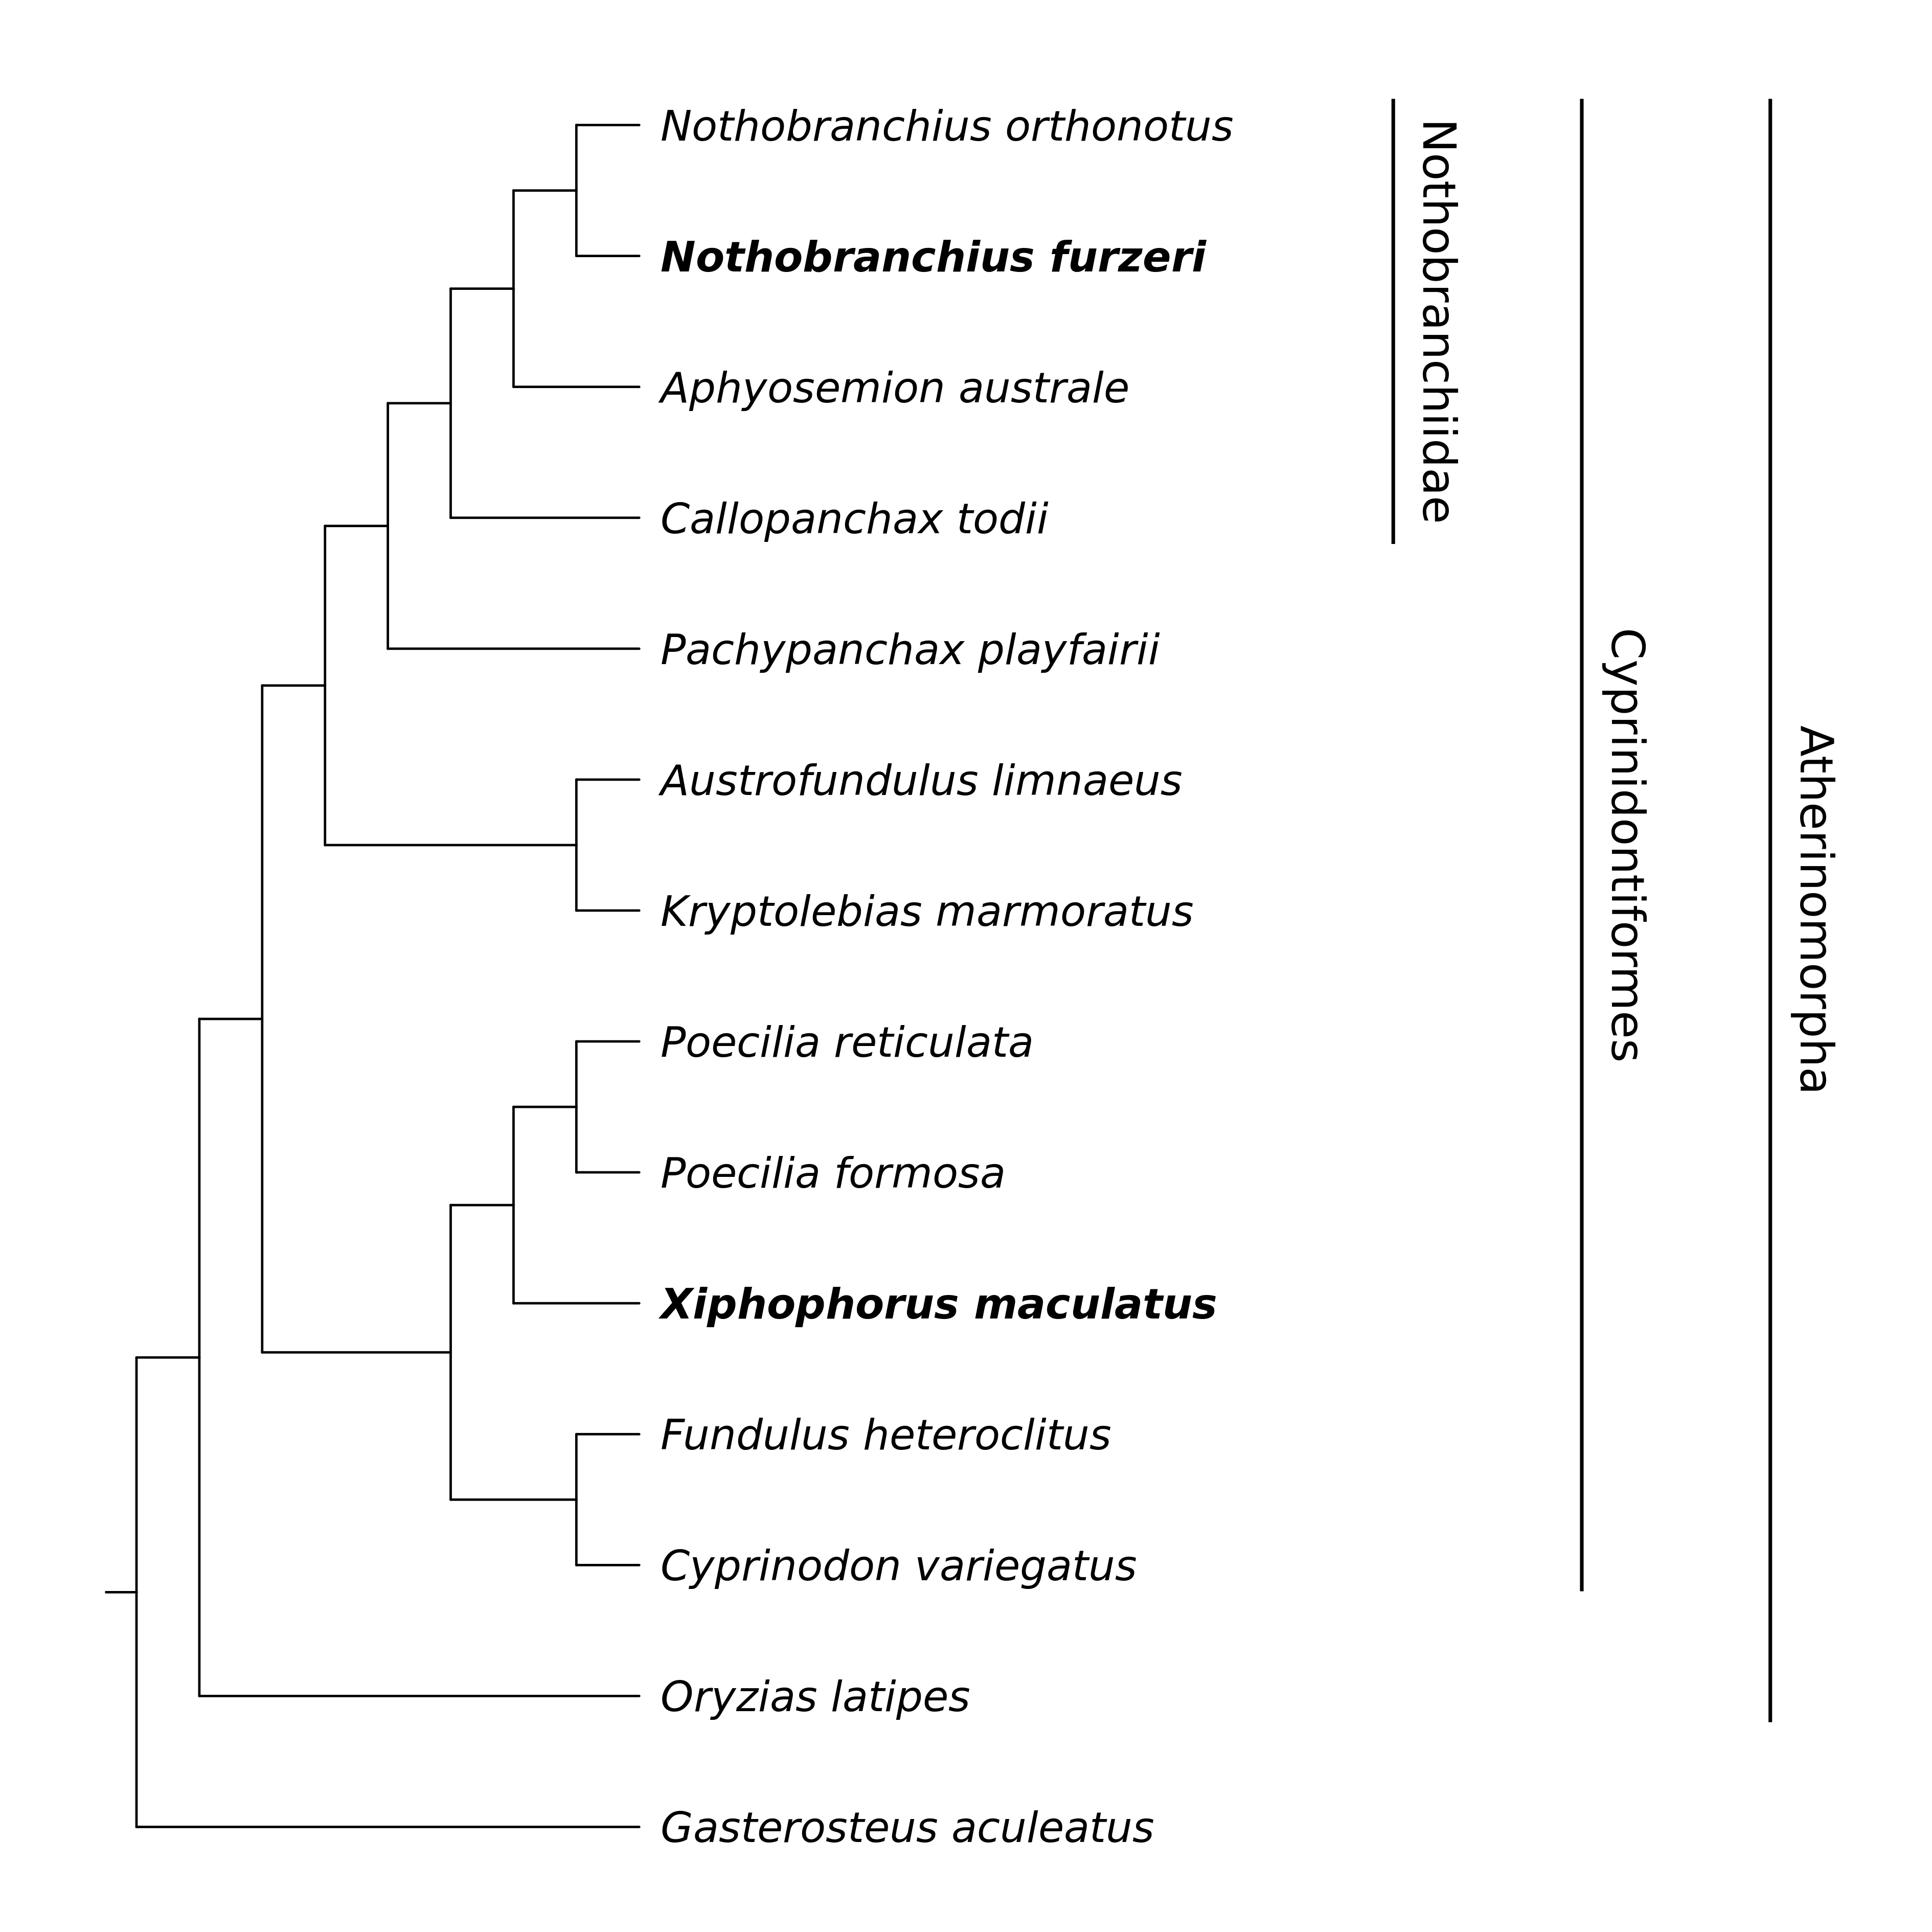
\includegraphics[width=0.9\textwidth]{_Figures/png/species-tree-large-taxa}
	\caption[Cladogram of analysed species]{\textbf{Cladogram of species included in this analysis.} Boldface type indicates species for which new, complete \igh{} locus assemblies were generated for this study; other species were either previously-characterised reference species (\species{G. aculeatus}, \species{O. latipes}) or underwent constant-region characterisation only (all other species). Labelled vertical bars designate higher taxa of interest.}
	\label{fig:species-tree-large-taxa}
\end{figure}

%%%%%%%%%%%%%%%%%%%%%%%%%%%%%%%%%%%%%%%%%%%%%%%%%%%%%%%%%%%%%%%%%%%%%%%%%%%%%%%
% KILLIFISH LOCUS SECTION
%%%%%%%%%%%%%%%%%%%%%%%%%%%%%%%%%%%%%%%%%%%%%%%%%%%%%%%%%%%%%%%%%%%%%%%%%%%%%%%

\section{The \igh{} locus of \nfu}
\label{sec:nfu-locus}

\subsection{Assembling the \Nfu \igh{} locus}
\label{sec:nfu-locus-assembly}

In order to locate and characterise the \nfu \igh{} locus, databases of \vh, \jh, and \ch exon sequences were collated from the published locus sequences of three reference species (zebrafish \parencite{danilova2005zebrafish}, three-spined stickleback \parencite{bao2010stickleback,gambondeza2011stickleback}, and medaka \parencite{magadan2011medaka}) and aligned to the \nfu genome (NFZ2.0) with \program{BLAST} \parencite{altschul1990blast,altschul1997blast}. Genome scaffolds with high-confidence alignments to at least two distinct segment types or covering at least 1\% of the scaffold's total length were retained for downstream analysis as potential locus candidates. In total, one chromosome (chr6) and 6 unincorporated scaffolds were identified as potentially covering part of the locus sequence (\Cref{tab:nfu-locus-scaffolds}), with chromosome 6 bearing the majority of identified gene segments.  %TODO: Add genome accession when available

\begin{table}[bh]
\centering
\caption{\Nfu genome scaffolds containing putative \igh{} locus fragments.}
\begin{threeparttable}
\begin{tabular}{cccccccc}\toprule
\textbf{Scaffold} & \textbf{Total length (kb)} & \textbf{V} & \textbf{J} & \textbf{\cm{}} & \textbf{\cd{}} & \textbf{\cz{}} & Included in locus?\\\midrule
chr6 & 6195.6 & 15 & 7 & 5 & 11 & 0 & Yes\\\midrule
scf10901 & 1.4 & 0 & 0 & 0 & 3 & 0 & Yes\\
scf21863 & 13.5 & 1 & 0 & 0 & 0 & 0 & No\\
scf35954 & 16.3 & 3 & 0 & 0 & 0 & 0 & No\\
scf36277 & 18.9 & 2 & 1 & 0 & 0 & 0 & No\\
scf37083 & 17.7 & 1 & 0 & 0 & 0 & 0 & No\\
scf9157 & 7.2 & 0 & 7 & 4 & 0 & 0 & Yes\\\bottomrule
\end{tabular}

\end{threeparttable}
\label{tab:nfu-locus-scaffolds}
\end{table}

\begin{table}[bh]
\centering
\caption{\Nfu BAC-library inserts containing putative \igh{} locus fragments.}
\begin{threeparttable}
\begin{tabular}{cccccccc}\toprule
\textbf{BAC ID} & \textbf{Insert length (kb)} & \textbf{V} & \textbf{J} & \textbf{\cm{}} & \textbf{\cd{}} & \textbf{\cz{}} & Included in locus?\\\midrule
154G24 & 106.6 & 17 & 1 & 0 & 0  & 0 & No\\
162F04 & 119.4 & 5  & 1 & 0 & 0  & 0 & No\\
165M01 & 110.7 & 15 & 1 & 0 & 0  & 0 & Yes\\
206K13 & 106.7 & 17 & 1 & 0 & 0  & 0 & No\\
208A08 & 103.2 & 17 & 1 & 0 & 0  & 0 & Yes\\
209K12 & 133.0 & 1  & 8 & 4 & 20 & 0 & Yes\\
220O06 & 104.8 & 4  & 1 & 0 & 0  & 0 & No\\
223M21 & 99.3  & 17 & 1 & 0 & 0  & 0 & No\\
248A22 & 47.3  & 7  & 0 & 0 & 0  & 0 & No\\
276N03 & 127.9 & 7  & 0 & 0 & 0  & 0 & Yes\\
277J10 & 120.8 & 17 & 1 & 0 & 0  & 0 & Yes\\
\bottomrule\end{tabular}

\end{threeparttable}
\label{tab:nfu-locus-bacs}
\end{table}

In order to determine which of the putative locus scaffolds were in fact part of the \igh{} locus, integrate these into a contiguous locus sequence, and provide additional information on any missing gene segments, bacterial artificial chromosome insert sequences from the killifish genome project BAC library \parencite{reichwald2015genome} were included in the locus assembly. BAC candidates, whose ends had already been sequenced as part of the genome project, were identified as potentially containing part of the locus sequence on the basis of their ends aligning to promising candidate scaffolds from a previous genome assembly (first round) or to the insert sequences of previously sequenced BAC inserts (second round). Once identified,  BAC candidates were isolated from culture by alkaline lysis, sequenced on an Illumina MiSeq sequencing machine, and assembled and scaffolded with \program{SPAdes} and \program{SSPACE}, respectively. Complete BAC insert assemblies were generated from these scaffolds by manual alignment to overlapping genome scaffolds and other BAC inserts, combined with PCR and Sanger sequencing of intervening sequences.

Finally, the assembled BAC inserts were screened for \igh{} locus segments in the same manner described for genome scaffolds, and passing insert sequences (\Cref{tab:nfu-locus-bacs}) were aligned to and integrated with the identified candidate scaffolds to produce a contiguous locus assembly. To minimise the probability of losing relevant gene segments to assembly errors, priority in the event of a sequence conflict between BACs and scaffolds was given first to any sequence containing a segment missing from the other; if neither the BAC assembly nor the genome scaffolds met this condition, priority was given to the genome scaffold over the BAC assembly. In total, 3 candidate scaffolds (including chromosome 6) and 5 BAC inserts were included in the final locus assembly, while 4 scaffolds and 6 BACs were excluded as likely representing isolated \igh{} orphon segments elsewhere in the genome. The correspondence between the final locus sequence and the sequences used to construct it is shown in \Cref{fig:nfu-locus-aln}.

\begin{figure}
\centering
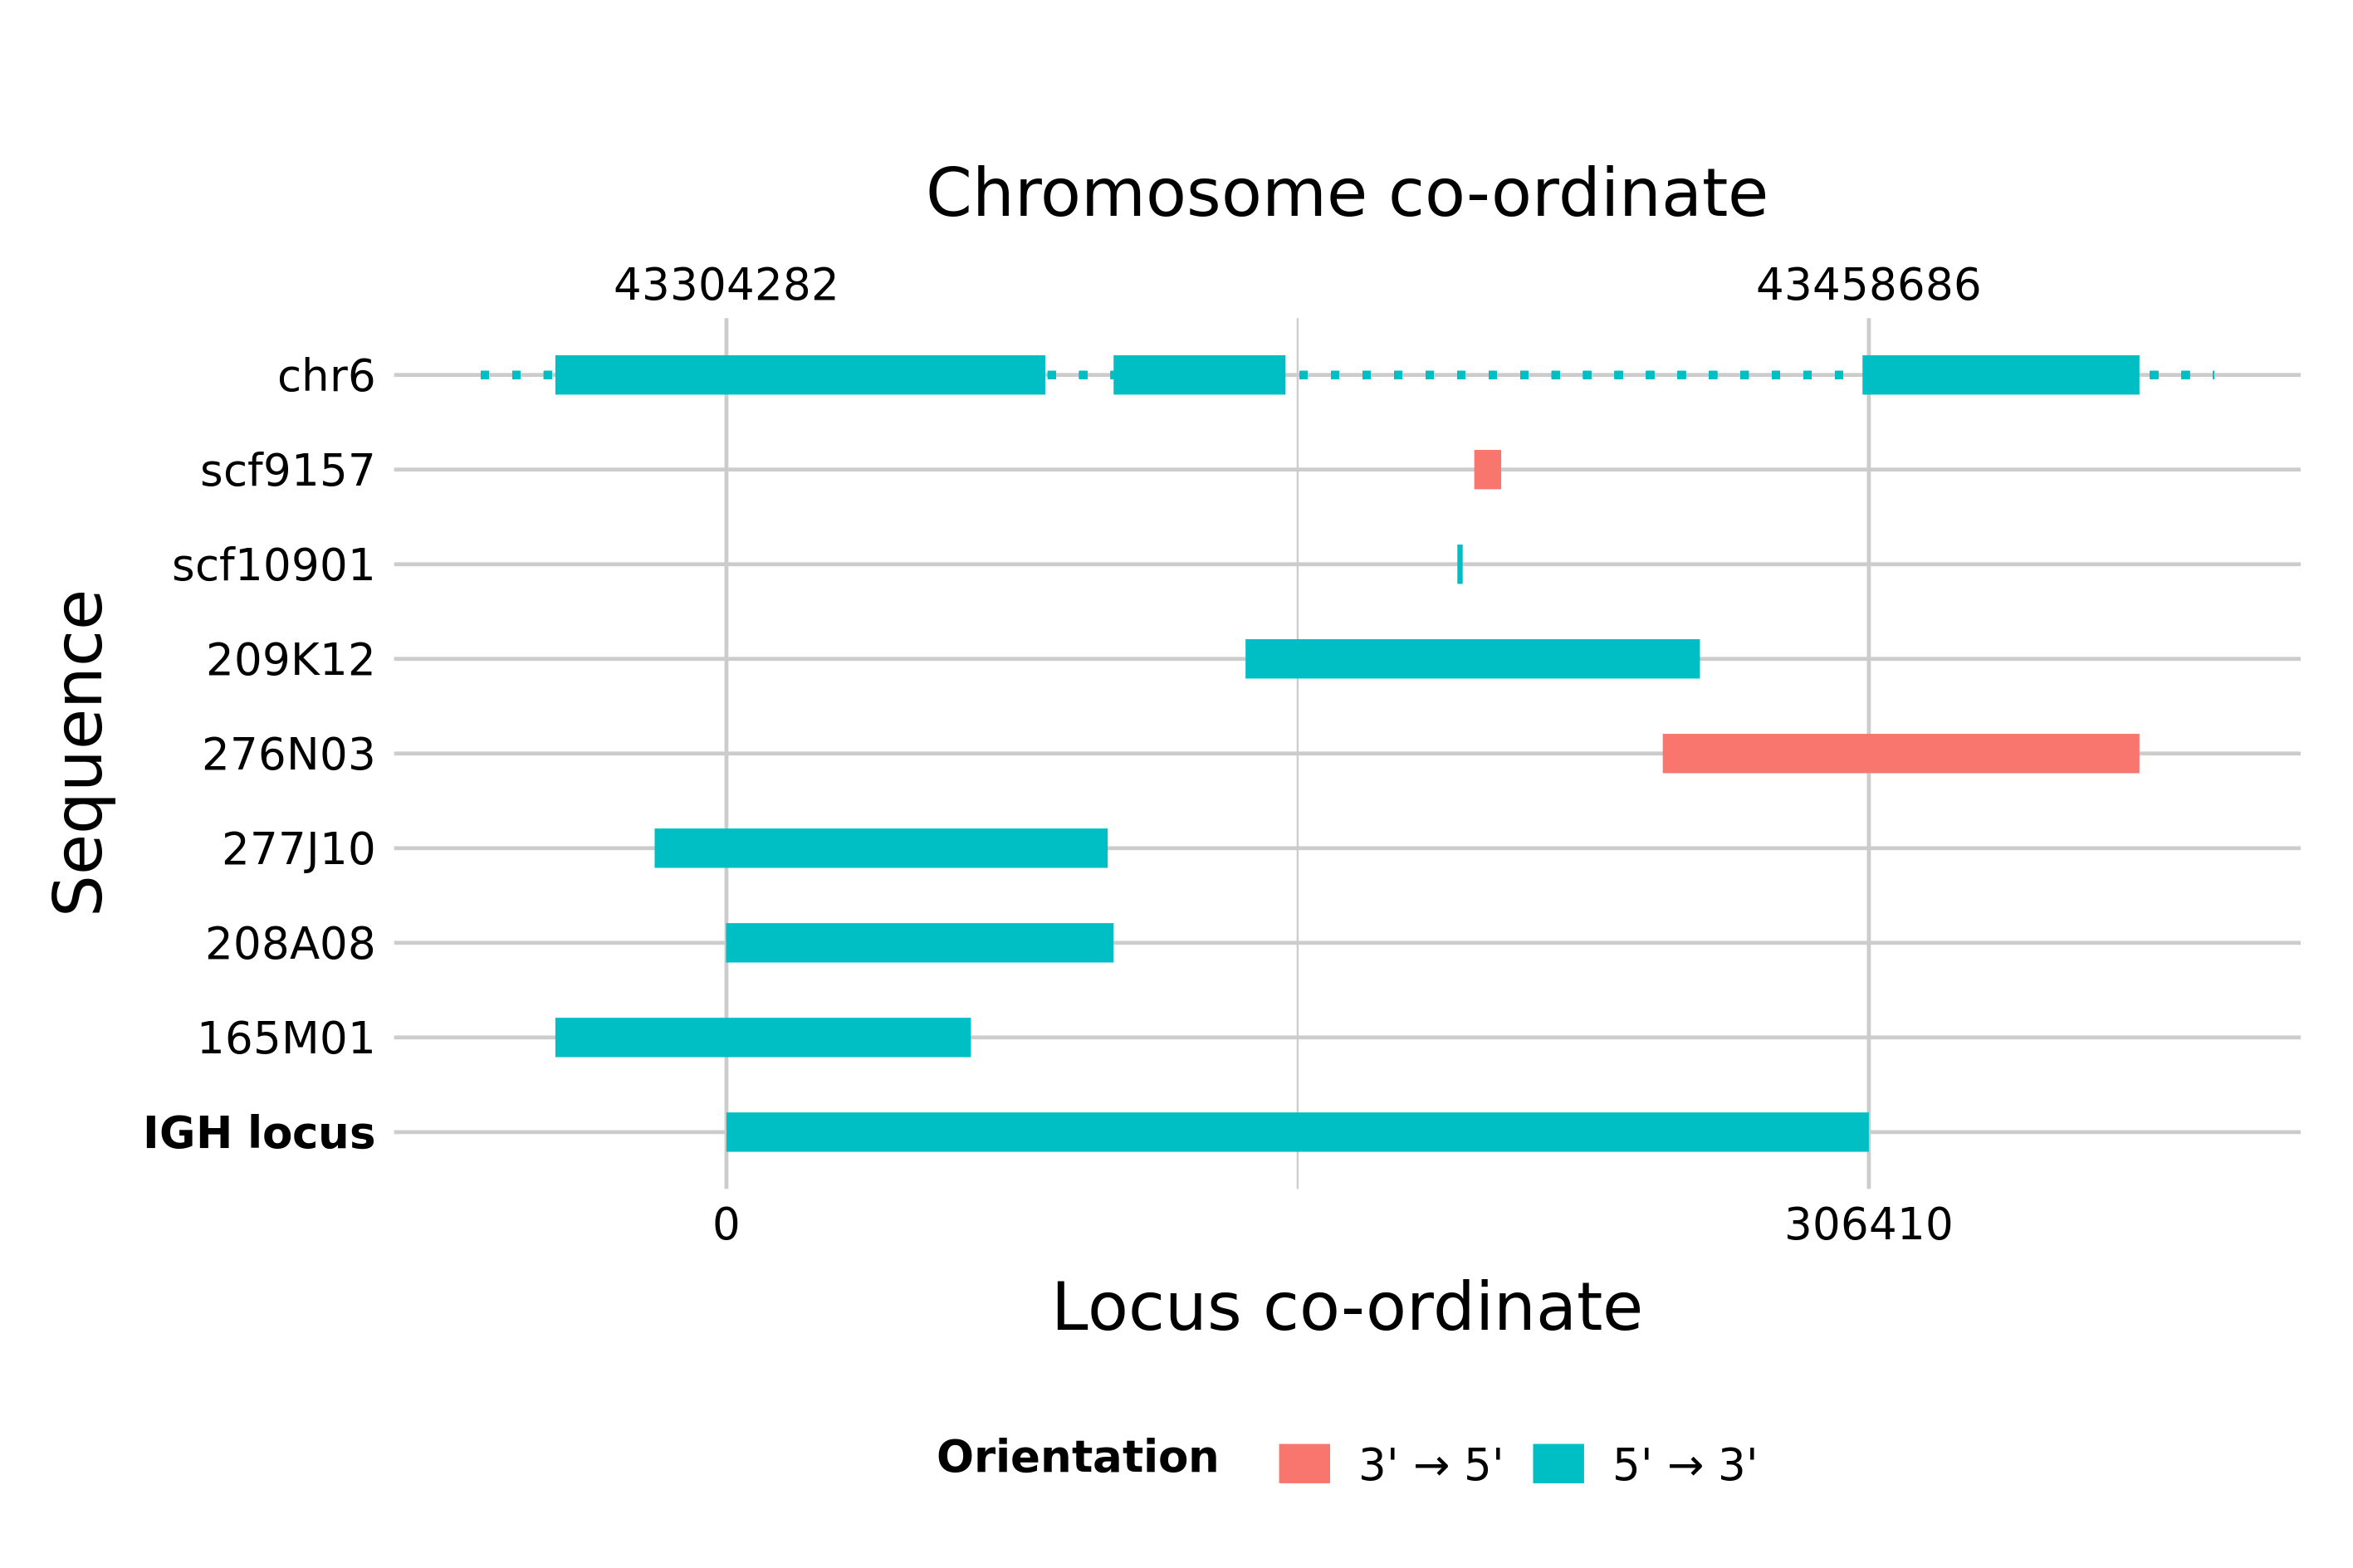
\includegraphics[width=\textwidth]{_Figures/png/nfu-locus-aln}
\caption[Assembling the \Nfu \igh{} locus]{\textbf{Assembling the \Nfu \igh{} locus:} Schematic of genome scaffolds and BAC inserts contributing to the \Nfu \igh{} locus sequence, with their corresponding place within the locus sequence (bottom axis). Internal gaps with dotted lines indicate locus regions with no corresponding locus sequence, as a result of intercalation of BAC or scaffold sequences.}
\label{fig:nfu-locus-aln}
\end{figure}

\subsection{Overall locus structure}
\label{sec:nfu-locus-structure}
	
The turquoise killifish genome contains a single \igh{} locus approximately 306 kilobases in length, located on chromosome 6 of the \Nfu genome (\Cref{fig:nfu-locus-map-a}). This locus comprises two complete subloci, \igh{1} (\kb{155}) and \igh{2} (\kb{118}), present in tandem and each occupying a classic {\vh-\dh-\jh-\ch} translocon configuration. This modified translocon structure, with multiple translocon subloci present in tandem, has been observed in a number of teleost \igh{} loci including catfish, medaka and stickleback \parencite{fillatreau2013astonishing}. Unusually, however, the smaller \igh{2} sublocus in \nfu \igh{} is present in antisense relative to the larger \igh{1}, with the two subloci beginning at opposite ends of the locus and facing each other in the middle (\Cref{fig:nfu-locus-map-b}). Such a multi-orientation locus structure has only previously been observed in medaka, the closest relative of the turquoise killifish to have its locus characterised prior to the present study \parencite{magadan2011medaka}; it is interesting to see this unusual feature reproduced here, raising the question of whether that this ideosyncracy is homologous between the two loci.
	
Compared to other closely-related loci, the killifish locus is relatively sparse and simple, with comparatively low functional complexity relative to its overall size. For example, whereas the stickleback locus fits four subloci, 49 V segments and 10 constant regions into c. \kb{200} \parencite{bao2010stickleback,gambondeza2011stickleback}, the killifish locus, despite being ~50\% longer, contains only 2 subloci, four constant regions and 24 V segments (including pseudogenised Vs). This difference results from the unusually large amount of nonfunctional sequence padding the killifish locus, resulting in large gaps between variable segments and in some cases between constant-region exons (\Cref{fig:nfu-locus-map-b}); this high prevalence of repetitive DNA is consistent with the rest of the TK genome, which comprises more than 60\% repetitive sequence \parencite{willemsen2019popgen}, compared to just over 15\% in stickleback \parencite{yuan2018repeats}. % TODO: Reference for Nfu repeat level - Cui et al ...
	
The two subloci in the turquoise killifish locus are generally highly similar in their functional sequence, with a high degree of synteny between their functional regions (\Cref{fig:nfu-locus-synteny}). The greatest degree of divergence occurs in the \vh and \dh regions, with what appear to be repeated deletion events in IGH2 resulting in a substantially lower number of \vh and \dh segments compared to IGH1; conversely, the \jh and constant regions are almost identical between two subloci. These patterns are discussed in more detail in \Cref{sec:nfu-locus-constant,sec:nfu-locus-variable}.
	
\begin{figure}
	\centering
	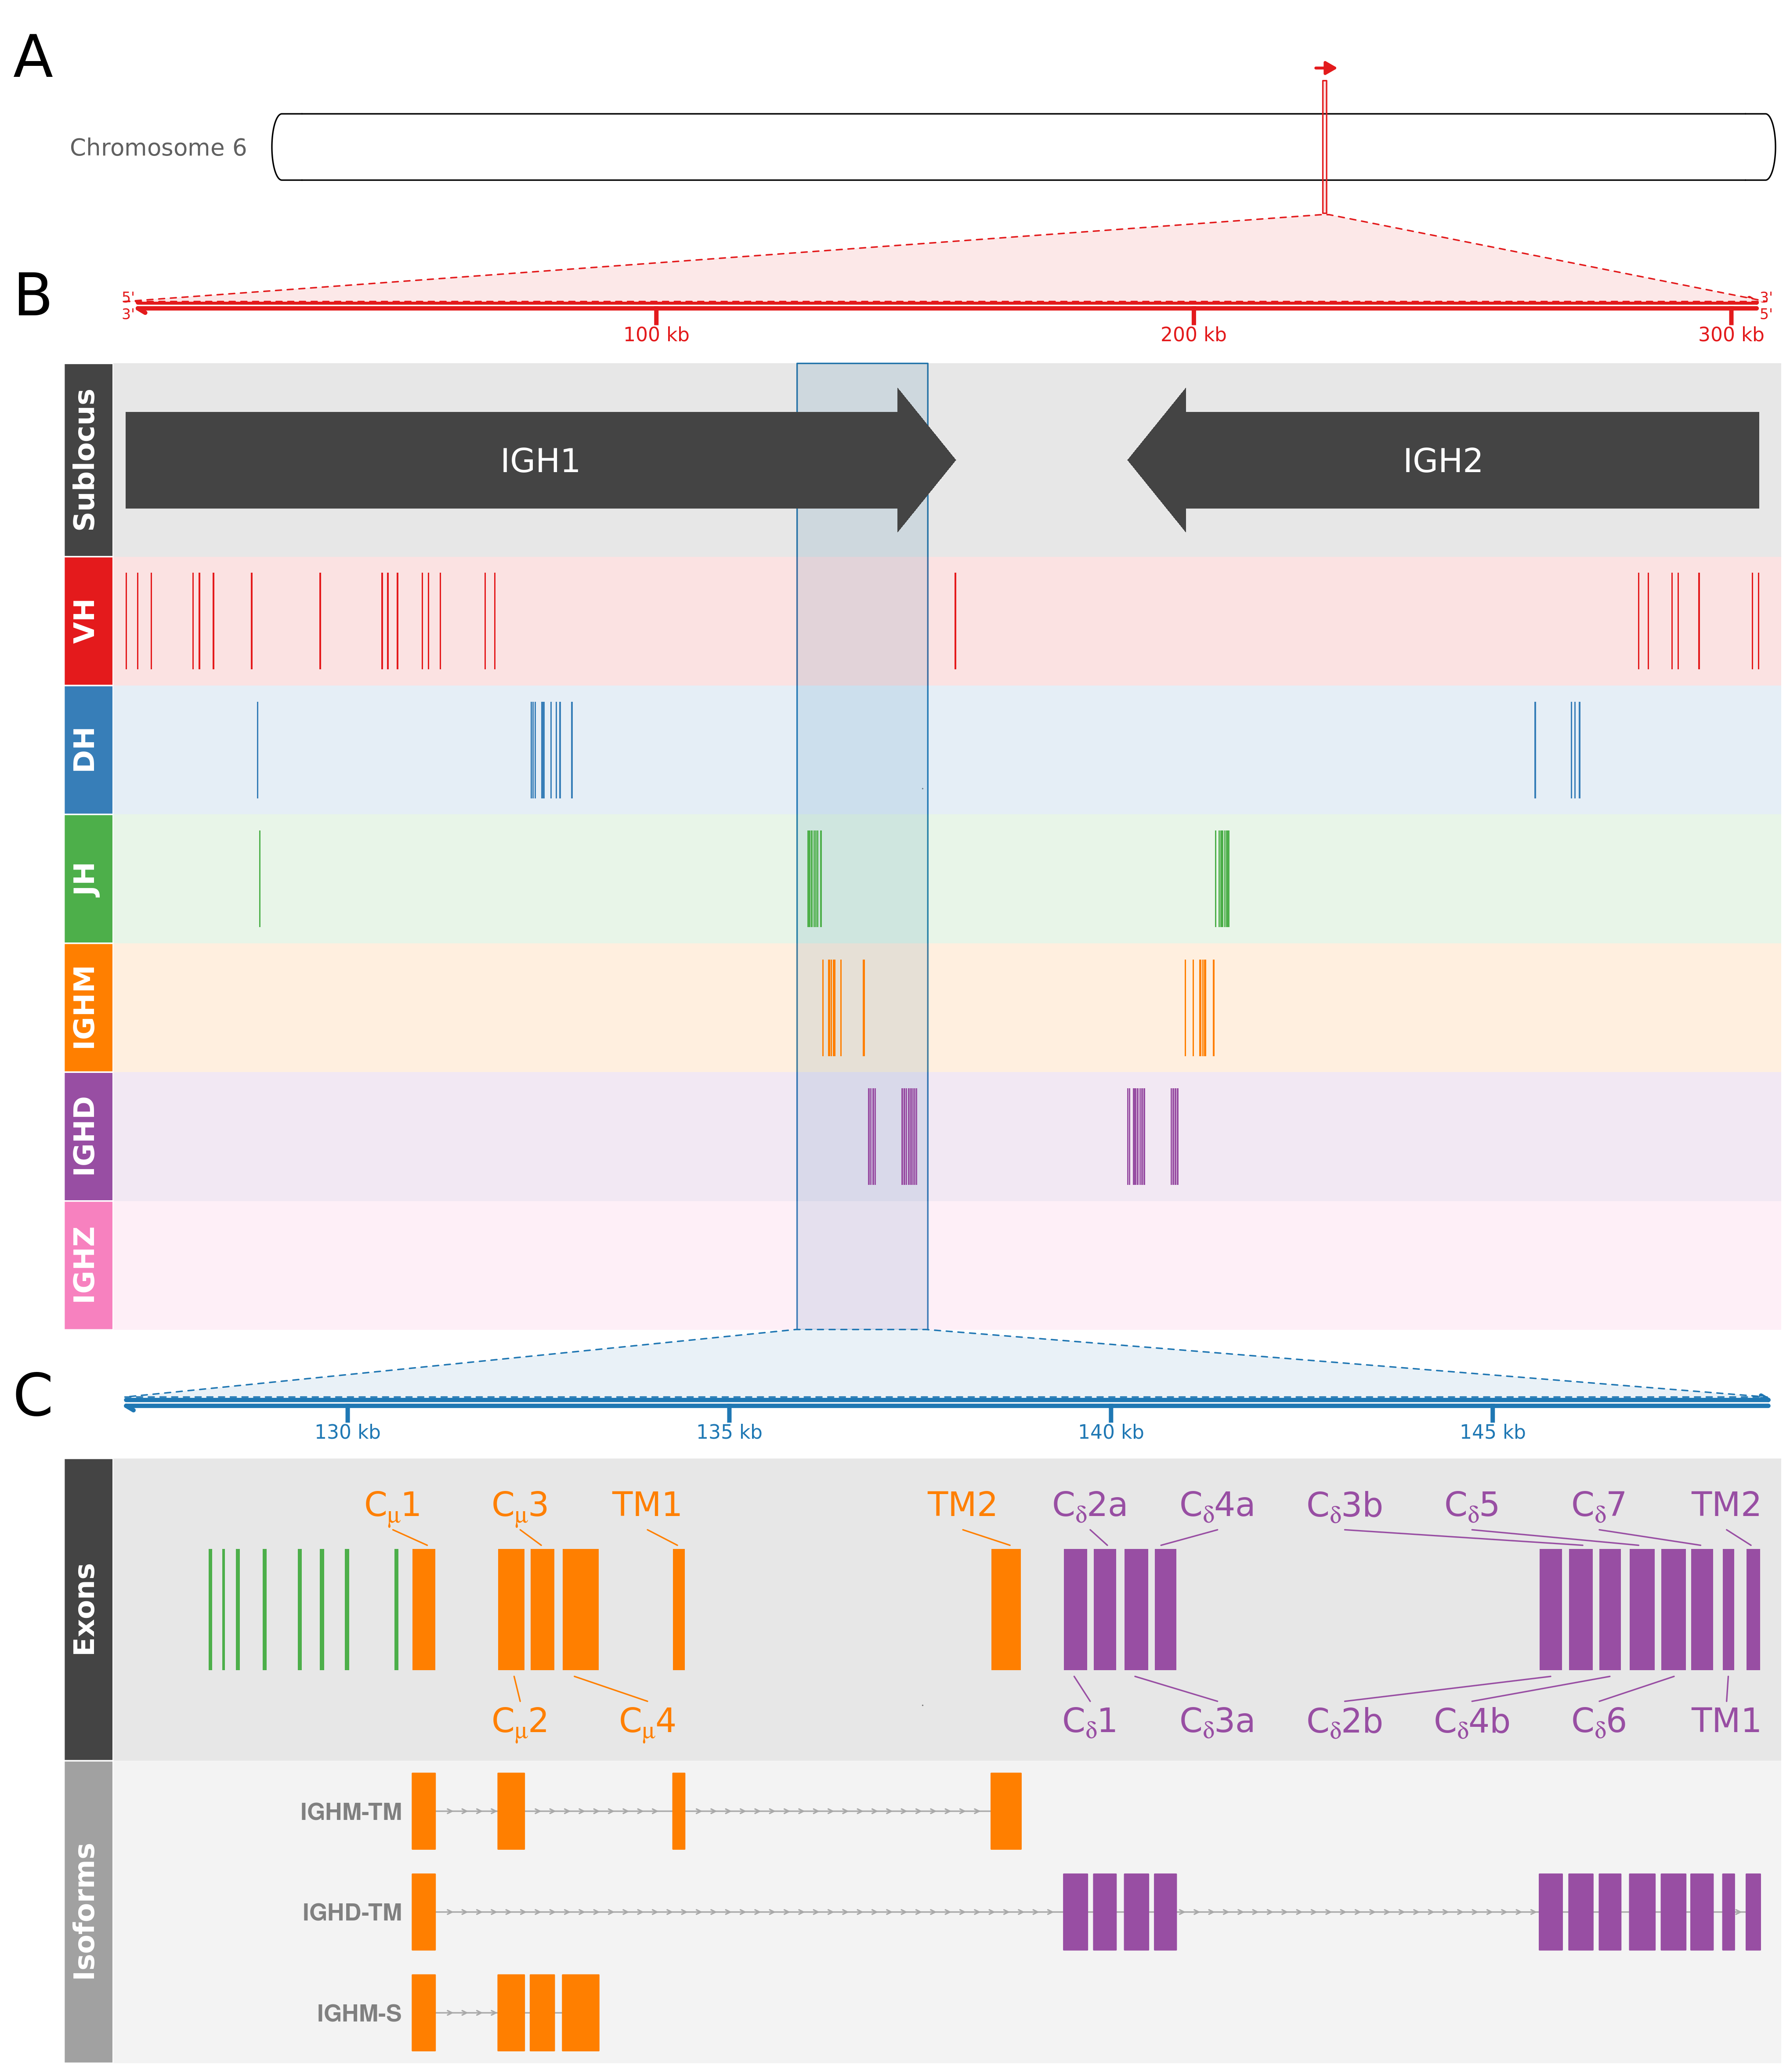
\includegraphics[width=\textwidth]{_Figures/png/nfu-locus-map}
			    \begin{subfigure}{0em}
        \phantomsubcaption{}
        \label{fig:nfu-locus-map-a}
    \end{subfigure}
    \begin{subfigure}{0em}
        \phantomsubcaption{}
        \label{fig:nfu-locus-map-b}
    \end{subfigure}
    \begin{subfigure}{0em}
        \phantomsubcaption{}
        \label{fig:nfu-locus-map-c}
        \end{subfigure}
	\caption[The immunoglobulin heavy chain (\igh{}) locus in \nfu]{\textbf{The immunoglobulin heavy chain (\igh{}) locus in \nfu:} (A) Position of the \igh{} locus on chromosome 6 of the \Nfu genome. (B) Arrangement of \vh, \dh, \jh and constant-region gene segments on the \Nfu \igh{} locus. All segments follow the orientation of their parent sublocus, indicated in the uppermost track. (C) Detailed map of the constant regions of the \textit{IGH1} sublocus, indicating the position and identity of the constant-region exons and the exon composition of expressed \igh{} isoforms in the turquoise killifish.}
	\label{fig:nfu-locus-map}
	\end{figure}
	
\begin{figure}
	\centering
	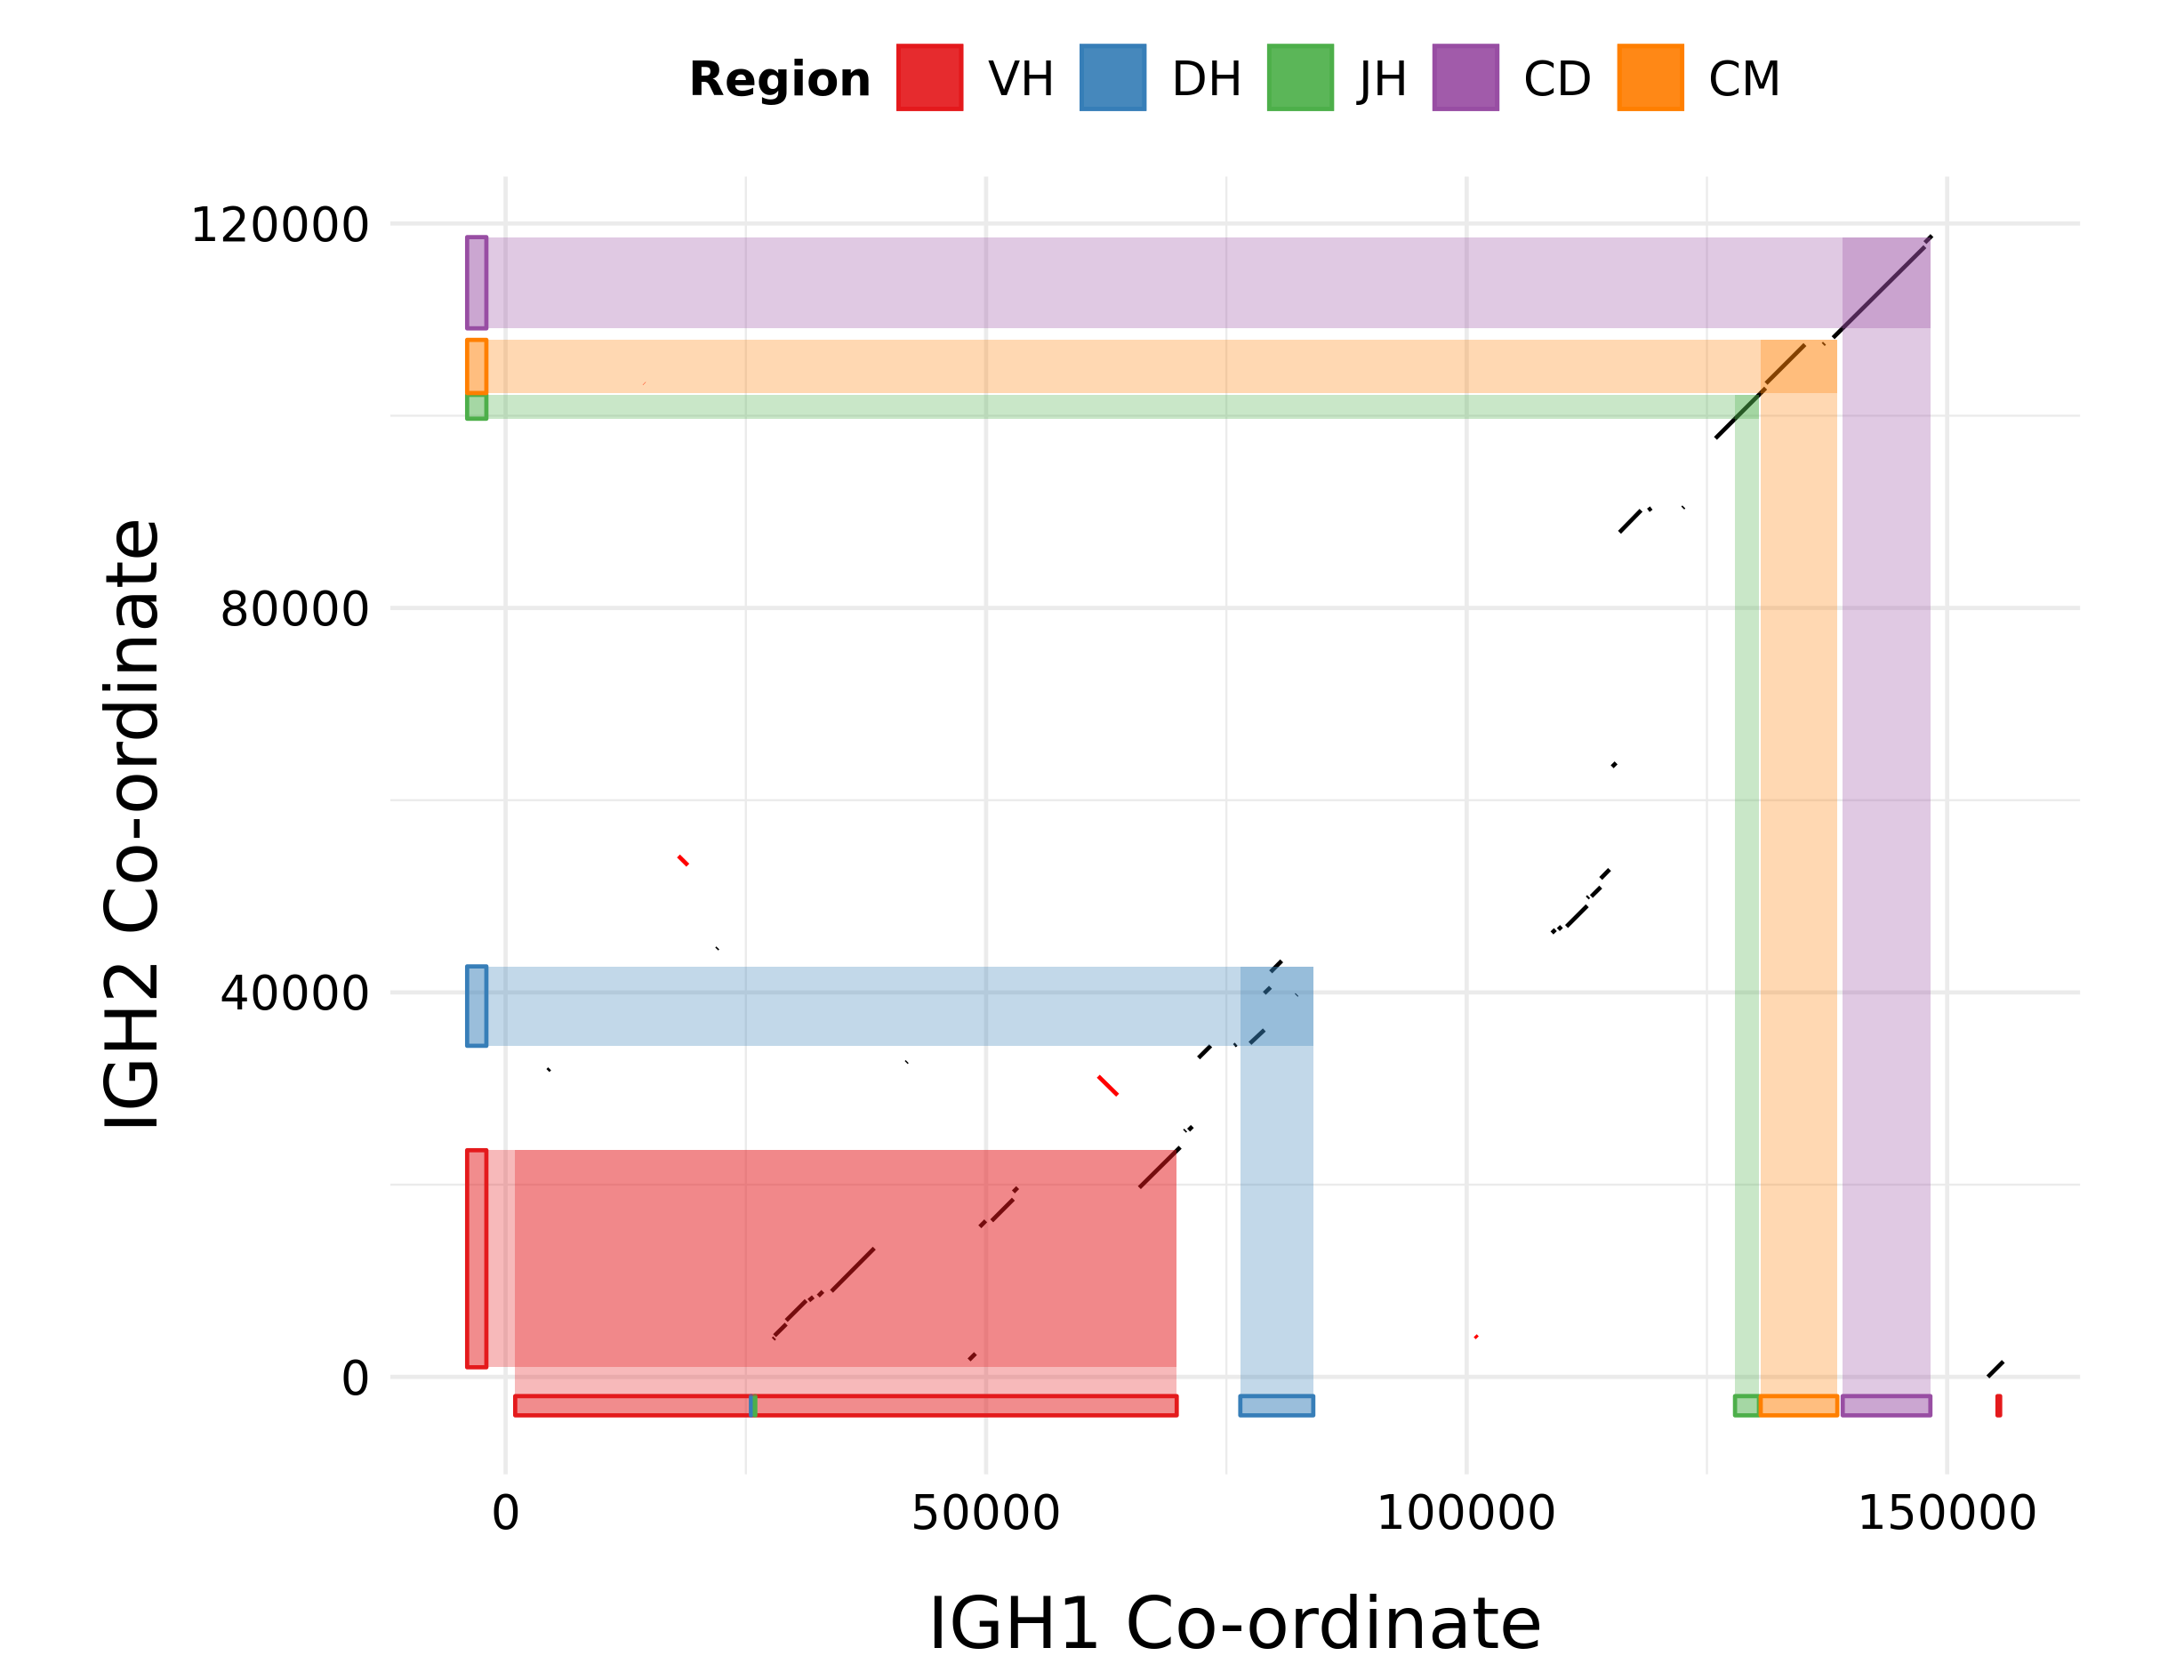
\includegraphics[width=0.9\textwidth]{_Figures/png/nfu-locus-dots}
	\caption[Sequence homology between subloci in \Nfu \igh{}]{\textbf{Sequence homology between subloci in \Nfu \igh{}:} Synteny plot of sequential best matches between \igh{1} and \igh{2} subloci, with gene segment regions indicated by coloured rectangles along each axis.}
	\label{fig:nfu-locus-synteny}
\end{figure}
	
	\subsection{Constant regions}
	\label{sec:nfu-locus-constant}
	
	The \textit{isotype} (also known as the \textit{class}) of an antibody determines its functional role within the immune system, including its possible effector functions and whether it can be secreted \parencite{schroeder2010immunoglobulins}. Three antibody isotypes have been identified to date in teleost fishes: \igh{M}, \igh{D} and \igh{Z} (a.k.a. \igh{T}, \igh{T/Z} or \igh{Z/T}) \parencite{fillatreau2013astonishing,bengten2015fishantibodies,magadan2015fishrepertoires}. Of these, \igh{M} and \igh{D} are highly primitive within the jawed vertebrates and found in most or all other vertebrate groups; within the teleosts, both appear to be universal \parencite{bengten2015fishantibodies}. Conversely, \igh{Z} is a teleost-specific isotype which is absent in other vertebrate taxa; within the teleosts, most characterised \igh{} loci possess \igh{Z}, but at least two (medaka and channel catfish) have been found to lack it \parencite{fillatreau2013astonishing,bengten2015fishantibodies}. In rainbow trout, \igh{Z} has been found to play a specialised mucosal role in the immune system analagous to that of \igh{A} in mammals \parencite{zhang2010igtgut,xu2013igtskin}, and it is widely assumed to play this specialised role throughout the teleosts; it is as yet unclear how mucosal immunity is effected in species lacking \igh{Z}.
	
	In order to investigate constant regions in the \nfu \igh{} locus, putative exon sequences were identified using \program{BLAST} alignments to the reference sequence databases described in \Cref{sec:nfu-locus-assembly}, and intron/exon bounderies were refined through alignment of published RNA-sequencing data from killifish gut (\parencite{smith2017microbiota}, BioProject accession PRJNA379208, young and old untreated groups) using \program{STAR} \Cref{fig:nfu-locus-sashimi}. Strikingly, the \nfu \igh{} locus appears to completely lack any \igh{Z} constant region, with no \cz{} exons or \igh{Z} transmembrane exons being found on either \igh{1} or \igh{2}. Given the widespread prevalence and specialised mucosal role of \igh{Z} in teleosts, its surprising absence in turquoise killifish (\Cref{fig:nfu-locus-map-b}) immediately raises questions about the nature, kinetics and efficacy of mucosal adaptive immunity in this species. The similar absence of \igh{Z} in medaka, which again is the closest relative of \Nfu with a characterised locus, raises further questions about the evolutionary history of \igh{Z} in the Atherinomorpha: does the shared absence of \igh{Z} in these species indicate a single ancestral deletion event, or parallel loss of this important isoform within both the Cyprinodontiformes (including the turquoise killifish) and Beloniformes (including medaka)? This latter question requires higher phylogenetic resolution to address effectively, and is investigated further in \Cref{sec:xma-locus} and \Cref{sec:comparative}.
	
	While \igh{Z} is completely missing from the \Nfu \igh{} locus, \igh{M}, the most primitive and widely-found isotype in jawed vertebrates, is present in its expected location, immediately downstream of the main \jh-region in both subloci. This constant region occupies the standard six-exon configuration, with four \cm{} exons and two transmembrane exons present in series on the chromosome (\Cref{fig:nfu-locus-map-b,fig:nfu-locus-map-c,fig:teleost-igm-exons-a}, \Cref{tab:nfu-ch-coords}). As with other species, both secreted and transmembrane isoforms of \igh{M} are present in the transcriptome, with secreted \igh{M} (\igh{M-S}) consisting of \cm{1-4} (\Cref{fig:nfu-locus-map-c,fig:nfu-locus-sashimi-a,fig:teleost-igm-exons-b}); however, the exon configuration of transmembrane \igh{M} (\igh{M-TM}) deviates from both that seen in mammals (in which exon TM1 is spliced to a cryptic splice site within \cm{4}) and most teleosts (in which the canonical splice site following \cm{3} is used and \cm{4} is excised) \parencite{fillatreau2013astonishing}. Rather, turquoise-killifsh \igh{M-TM} resembles that of medaka, in which both \cm{3} and \cm{4} are excluded and the canonical splice site at the end of \cm{2} is spliced directly to TM1 (\Cref{fig:teleost-igm-exons-c,fig:teleost-igm-exons-d,fig:teleost-igm-exons-e}). This similarity to medaka again raises the possibility that this unusual feature may be a conserved feature of both lineages; however, the underlying mechanism giving rise to this difference in splicing behaviour is unknown.
	
		Unlike \igh{M}, the exon structure of \igh{D} is highly variable across the teleosts, ranging from roughly 7-17 \cd{} exons in addition to the transmembrane domains \parencite{fillatreau2013astonishing}. The core structure of \igh{D} comprises seven \cd{} exons (\cd{1-7}), but some subset of these exons may be missing or duplicated in any given species -- in medaka, for example, \cd{5} is missing in all subloci \parencite{magadan2011medaka}, while in many species (e.g. zebrafish, salmon, and channel catfish) \cd{2-4} are duplicated in two or more tandem blocks \parencite{fillatreau2013astonishing}. This latter configuration is also observed in turquoise killifish, in which the \igh{D} constant region immediately follows \igh{M} in both subloci and has a 

\cd{1}-(\cd{2}-\cd{3}-\cd{4})$_2$-\cd{5}-\cd{6}-\cd{7}-TM1-TM2 

	\noindent configuration, for a total of 12 exons per \igh{D} constant region (\Cref{fig:nfu-locus-map-b,fig:nfu-locus-map-c}, \Cref{tab:nfu-ch-coords}). All of these exons appear to be expressed in tandem, resulting in a much longer transcript than is observed for any isoform of \igh{M} (\Cref{fig:nfu-locus-map-c,fig:nfu-locus-sashimi-b}). As in other teleost species, \igh{D} in the turquoise killifish includes a chimeric \cm{1} exon at the 5' end of the constant-region transcript, for a total of 13 exons per \igh{D-TM} mRNA (\Cref{fig:nfu-locus-sashimi-b}).

	While the best-known form of \igh{D} in teleosts is transmembrane, secreted \igh{D} has been observed in at least two teleost species, with different mechanisms used in each case: in channel catfish, one dedicated sublocus has a dedicated IgD secretory exon in place of the transmembrane exons \parencite{bengten2006catfish}, while in rainbow trout (and possibly some other species like Atlantic salmon and cod) a run-on event at the end of \cd{7} results in the production of a secretory tail in a manner similar to secretory IgZ \parencite{ramirezgomez2012secretoryigd}. However, neither a specialised secretory exon nor a \cd{7} secretory tail could be detected in turquoise killifish, suggesting that IgD may only be expressed in transmembrane form in this species.
	
	In the case of both \igh{M} and \igh{D}, the constant regions are present in their expected configuration in each sublocus and are highly similar in sequence between the subloci, with an average of 98.4\% nucleotide sequence identity for corresponding IgM exons and 99.3\% for corresponding IgD exons (\Cref{fig:nfu-ch-aln} and \Cref{tab:nfu-ch-aln}) in pairwise Needleman-Wunsch alignments \parencite{needleman1970align}. This high level of similarity indicates either a very recent duplication event to produce the second sublocus or a high level of sequence conservation in both subloci, with the latter explanation suggesting that both subloci continue to be functional and active in the immune system.
	
	\begin{figure}
	\centering
		    \begin{subfigure}{0em}
        \phantomsubcaption{}
        \label{fig:teleost-igm-exons-a}
    \end{subfigure}
    \begin{subfigure}{0em}
        \phantomsubcaption{}
        \label{fig:teleost-igm-exons-b}
    \end{subfigure}
    \begin{subfigure}{0em}
        \phantomsubcaption{}
        \label{fig:teleost-igm-exons-c}
    \end{subfigure}
    \begin{subfigure}{0em}
        \phantomsubcaption{}
        \label{fig:teleost-igm-exons-d}
    \end{subfigure}
    \begin{subfigure}{0em}
        \phantomsubcaption{}
        \label{fig:teleost-igm-exons-e}
    \end{subfigure}
	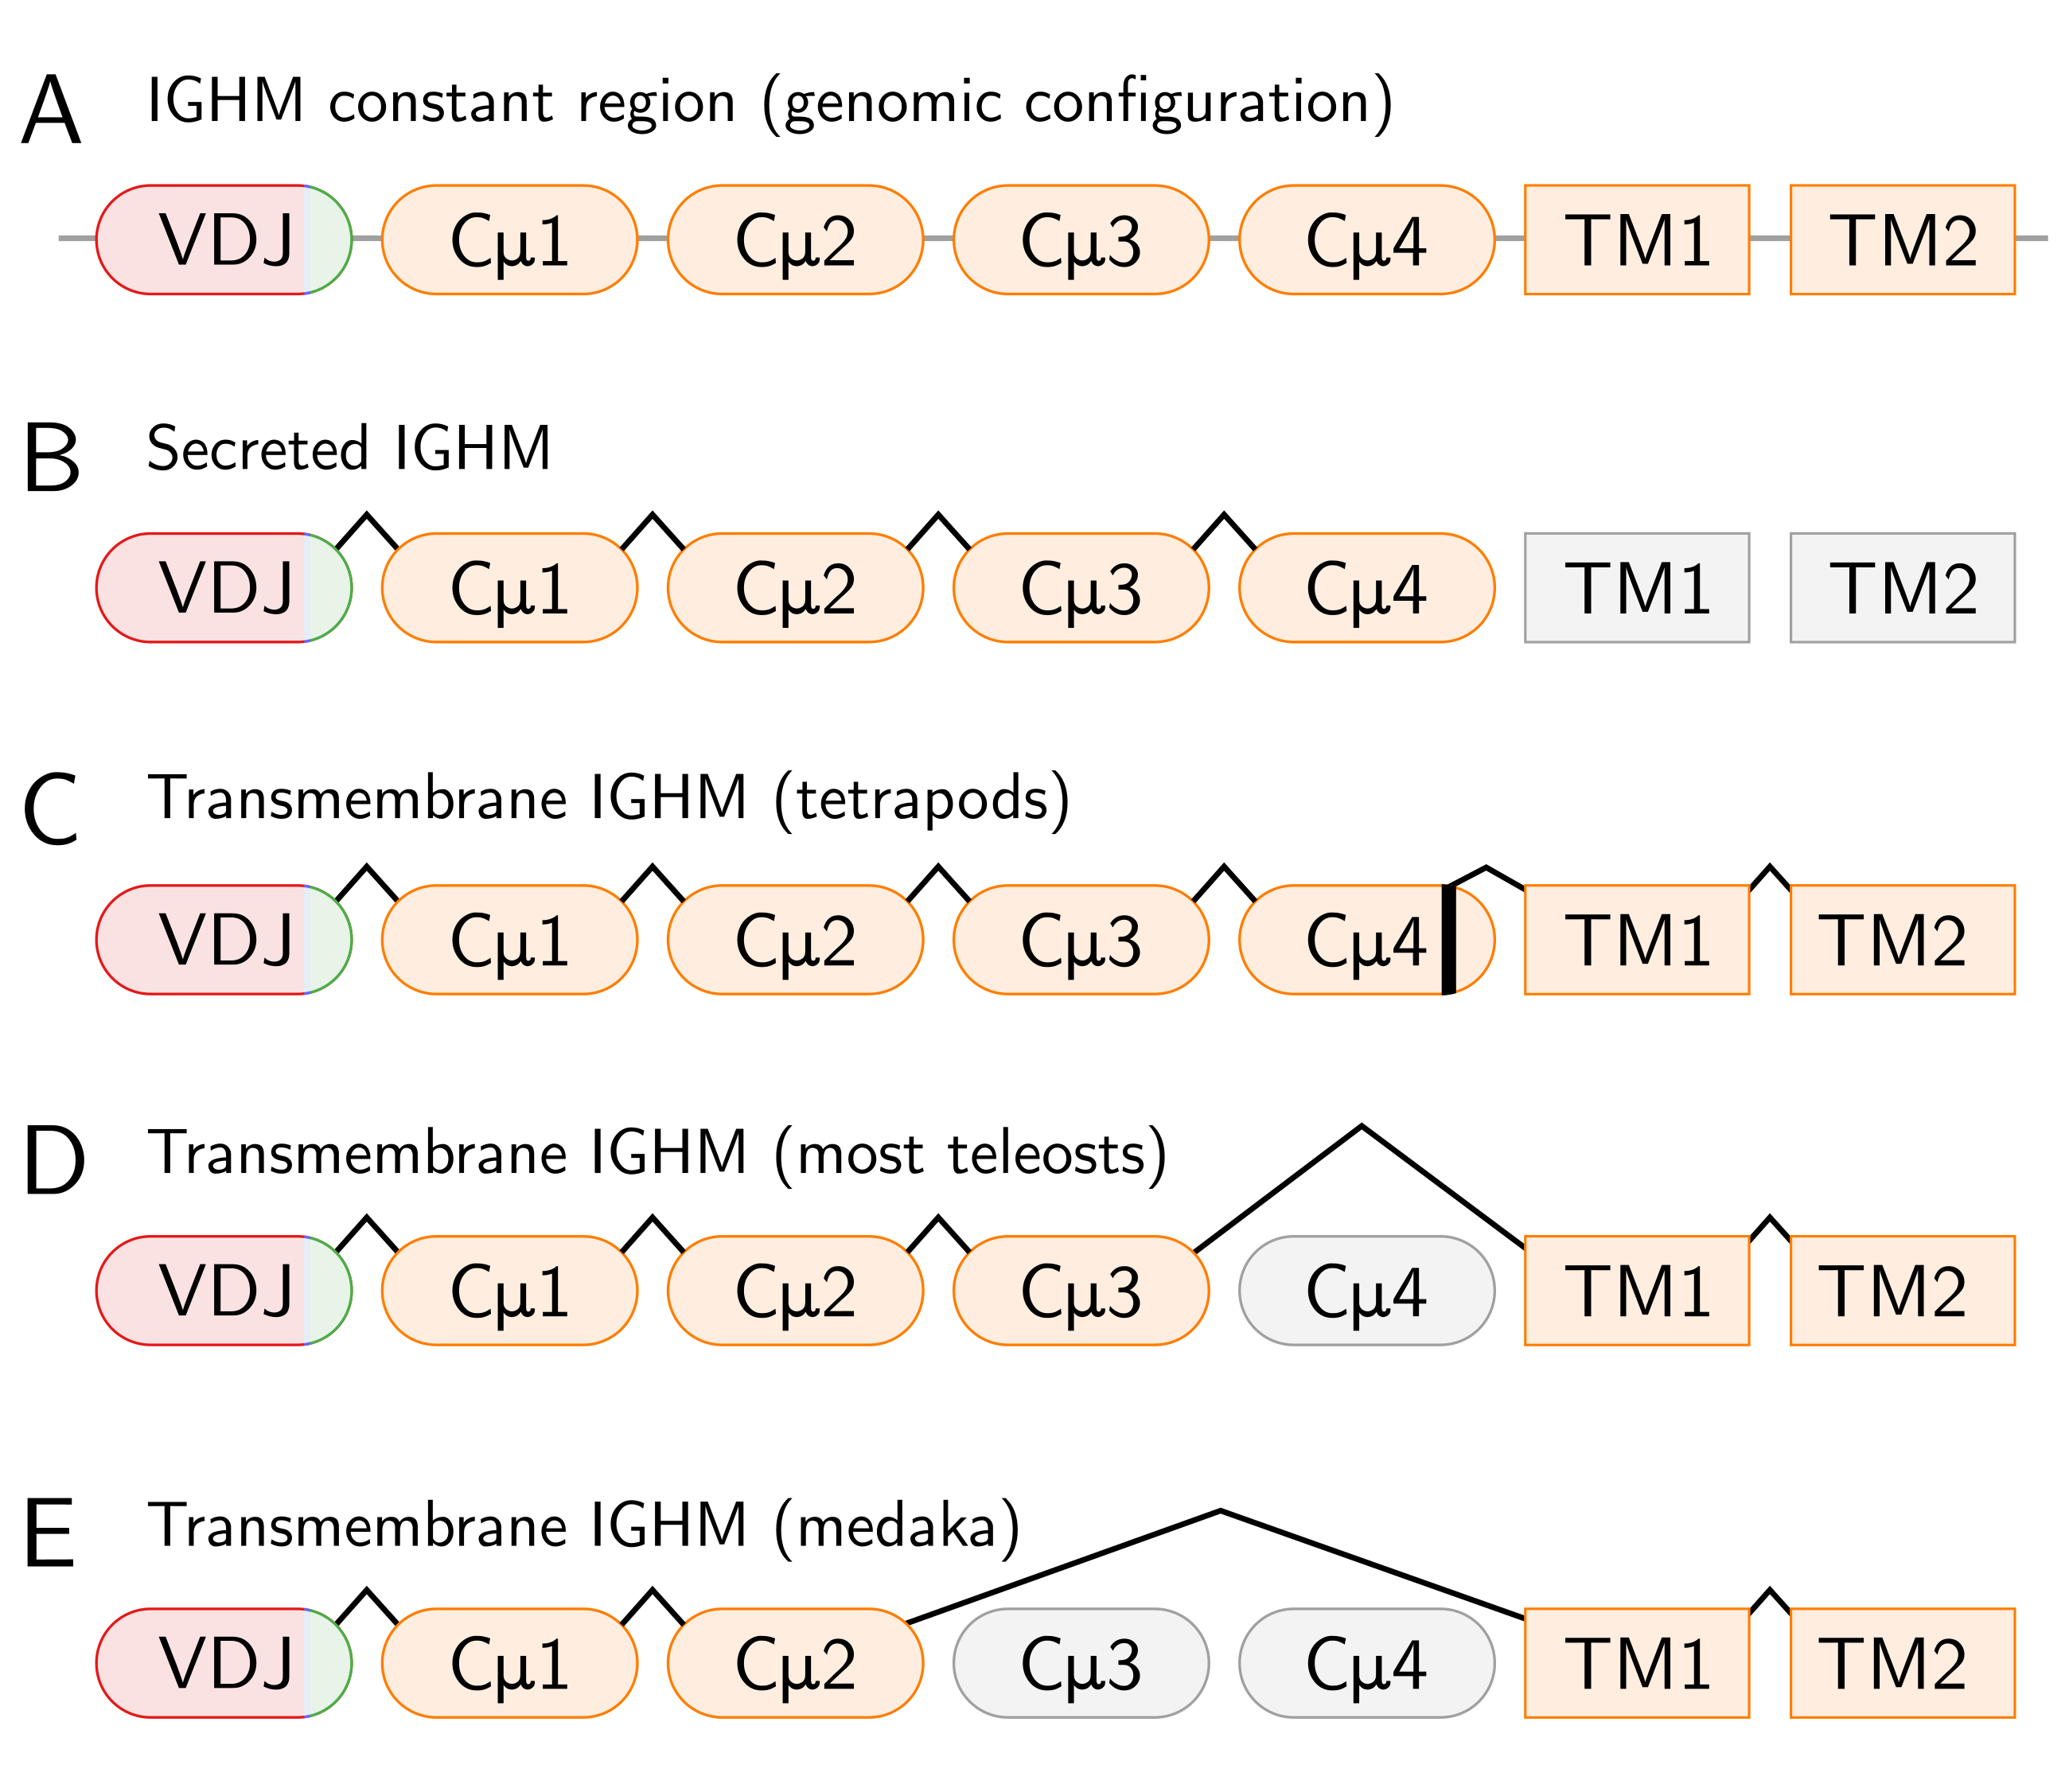
\includegraphics[width=0.8\textwidth]{_Figures/png_edited/teleost-igm-exons}
	\caption[IgM exon usage in other vertebrates]{\textbf{\igh{M} exon usage in other vertebrates:} Schematic of \igh{M} splice patterns in different isoforms and taxonomic groups; (A) standard genomic (pre-splicing) configuration of \igh{M}, following VDJ recombination; (B) exon configuration of secreted \igh{M} (\igh{M-S}) in tetrapods and teleosts; (C) exon configuration of transmembrane \igh{M} (\igh{M-TM}) in tetrapods, demonstrating the use of a cryptic splice site in \cm{4}; (D) standard \igh{M-TM} exon configuration in teleosts, demonstrating the direct splicing of \cm{3} to TM1 and exclusion of \cm{4}; (E) unusual \igh{M-TM} exon configuration observed in medaka, in which both \cm{3} and \cm{4} are excluded. Figure adapted from Fillatreau \textit{et al.} (2013).}
	\label{fig:teleost-igm-exons}
	\end{figure}
	
	\begin{figure}
	\centering
		\begin{subfigure}{0em}
        \phantomsubcaption{}
        \label{fig:nfu-locus-sashimi-a}
    \end{subfigure}
    \begin{subfigure}{0em}
        \phantomsubcaption{}
        \label{fig:nfu-locus-sashimi-b}
    \end{subfigure}
	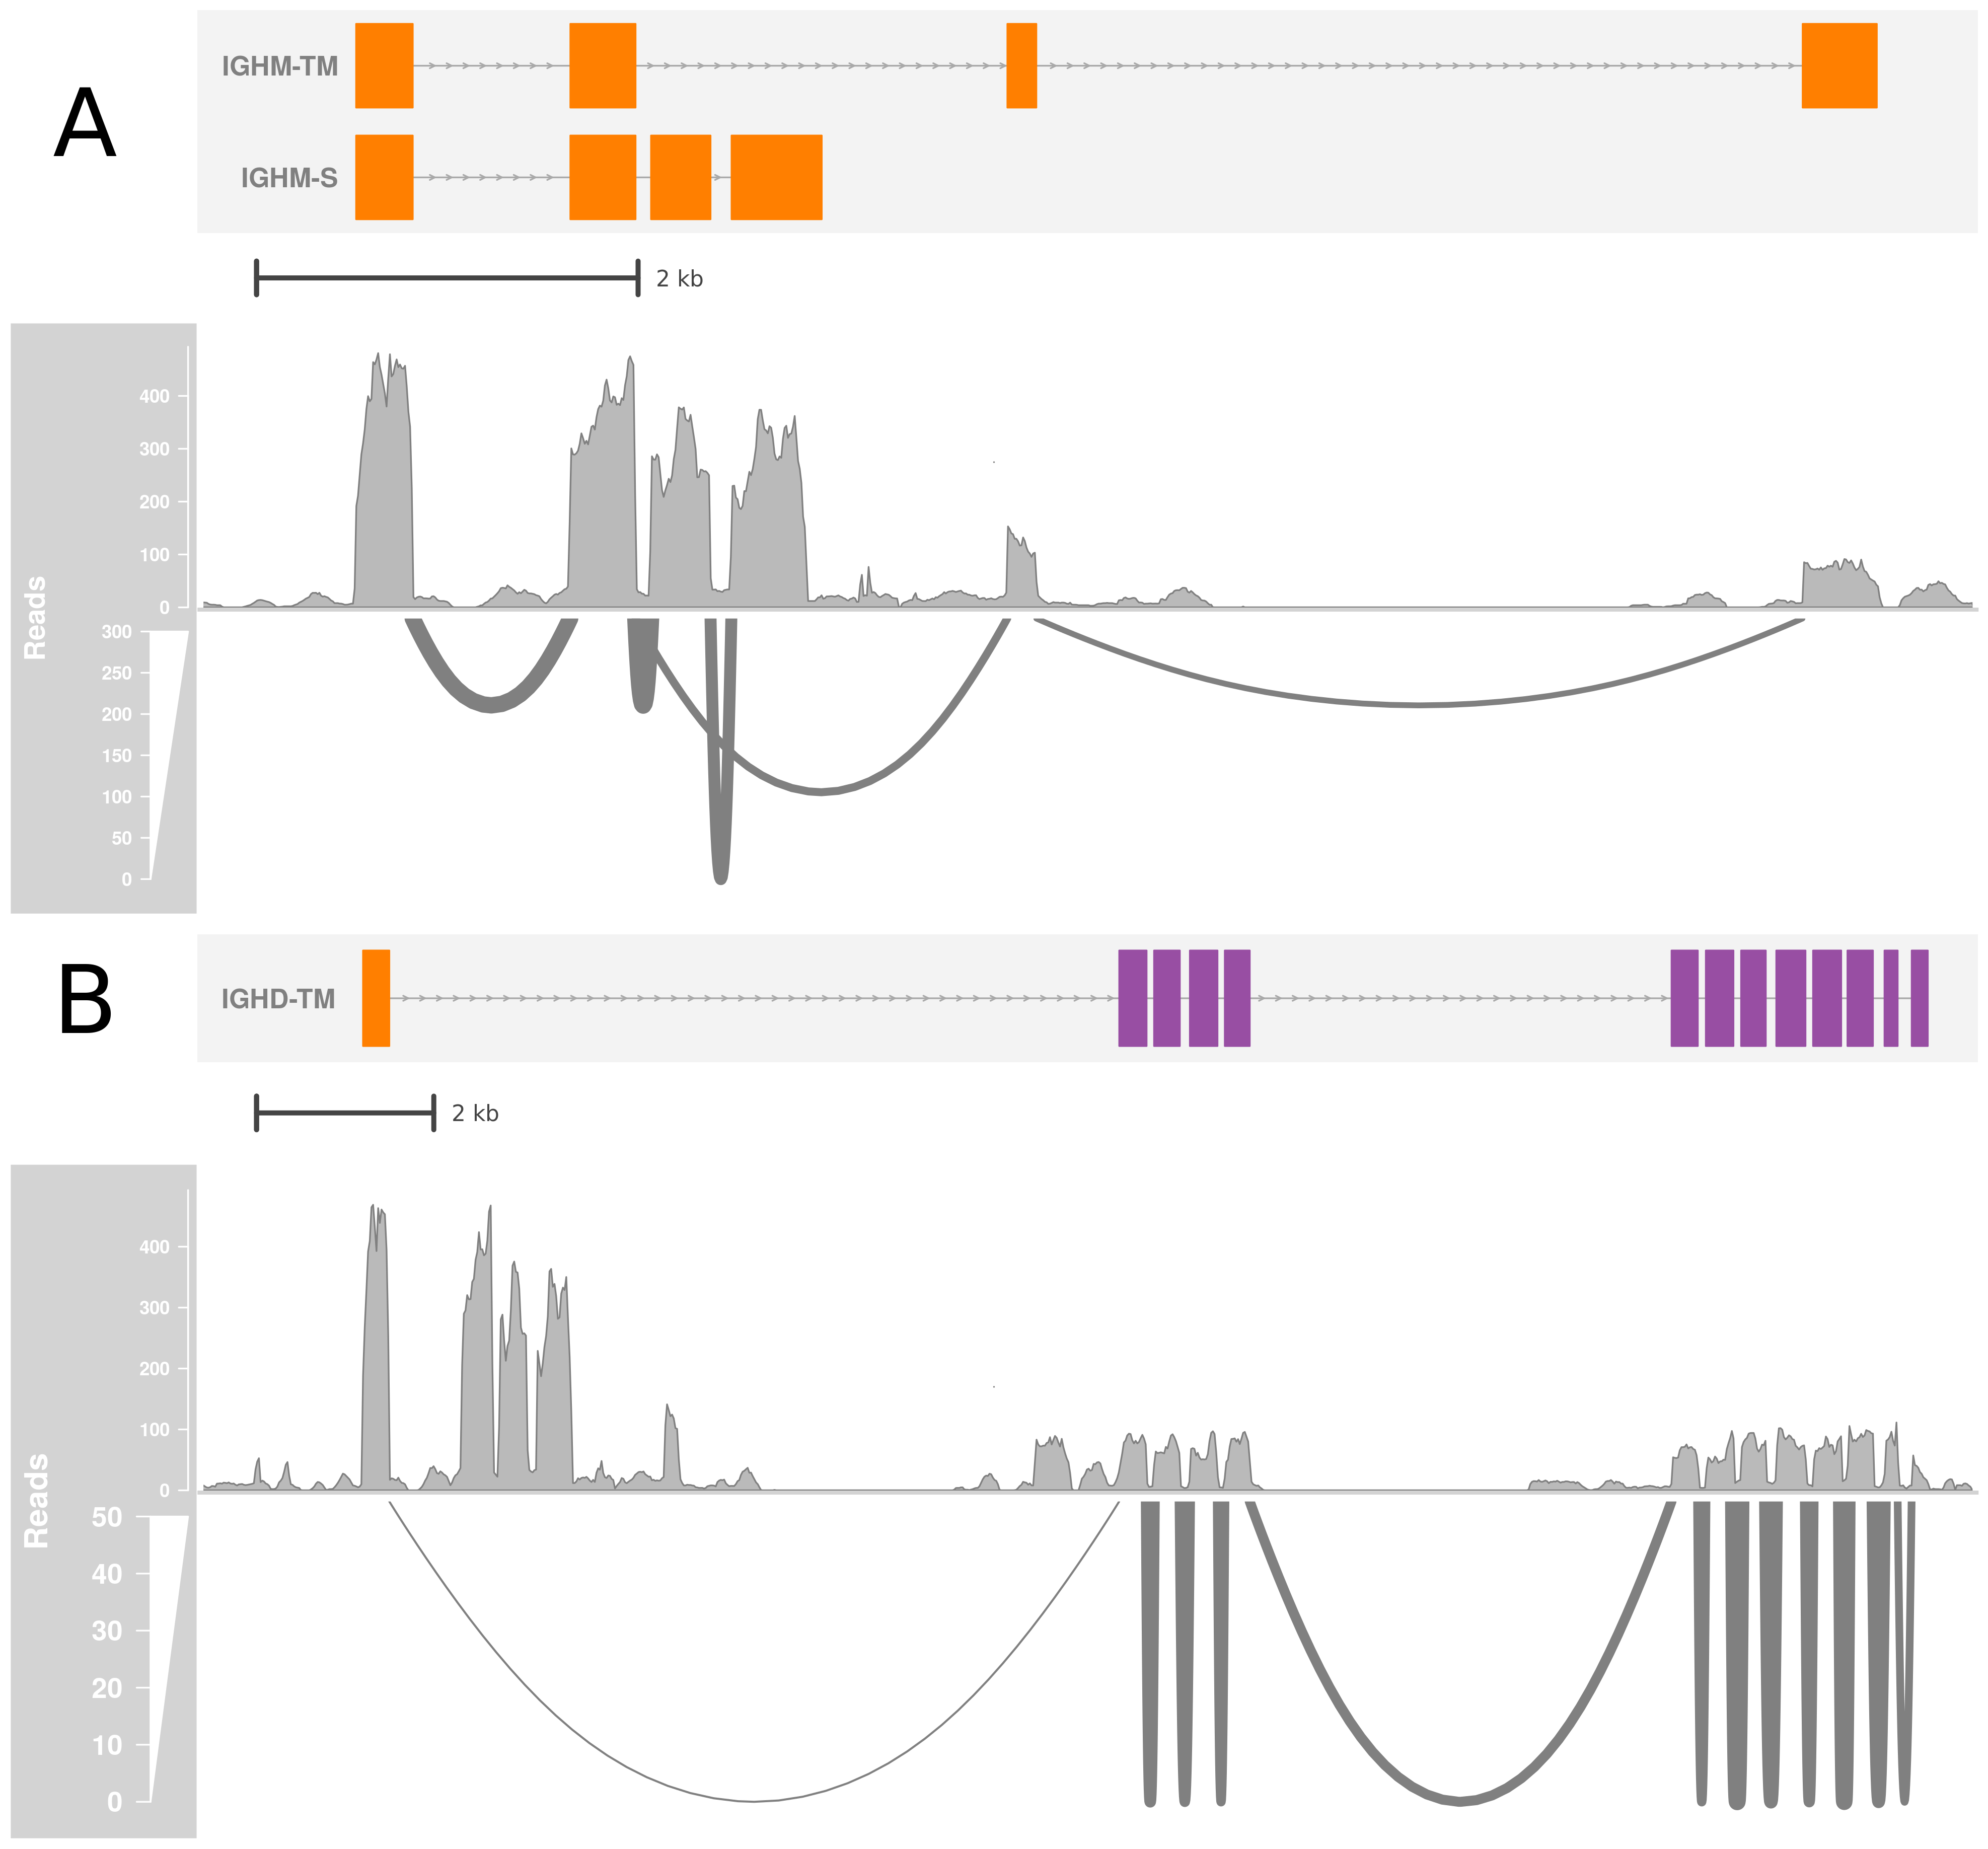
\includegraphics[width=\textwidth]{_Figures/png/nfu-locus-sashimi}
	\caption[Constant-region isoforms in \Nfu]{\textbf{Constant-region isoforms in \Nfu:} Coverage and sashimi plots of \program{STAR}-aligned RNA-seq reads from \Nfu gut samples \parencite{smith2017microbiota}, demonstrating the splicing behaviour of \igh{1} constant-region isoforms. (A) \igh{M} exon splicing, showing alternative splicing patterns of \igh{M-TM} and \igh{M-S}; (B) \igh{D} exon splicing, including chimeric splicing of \cm{1} to \cd{1}.}
	\label{fig:nfu-locus-sashimi}
	\end{figure}
	
	\begin{figure}
	\centering
	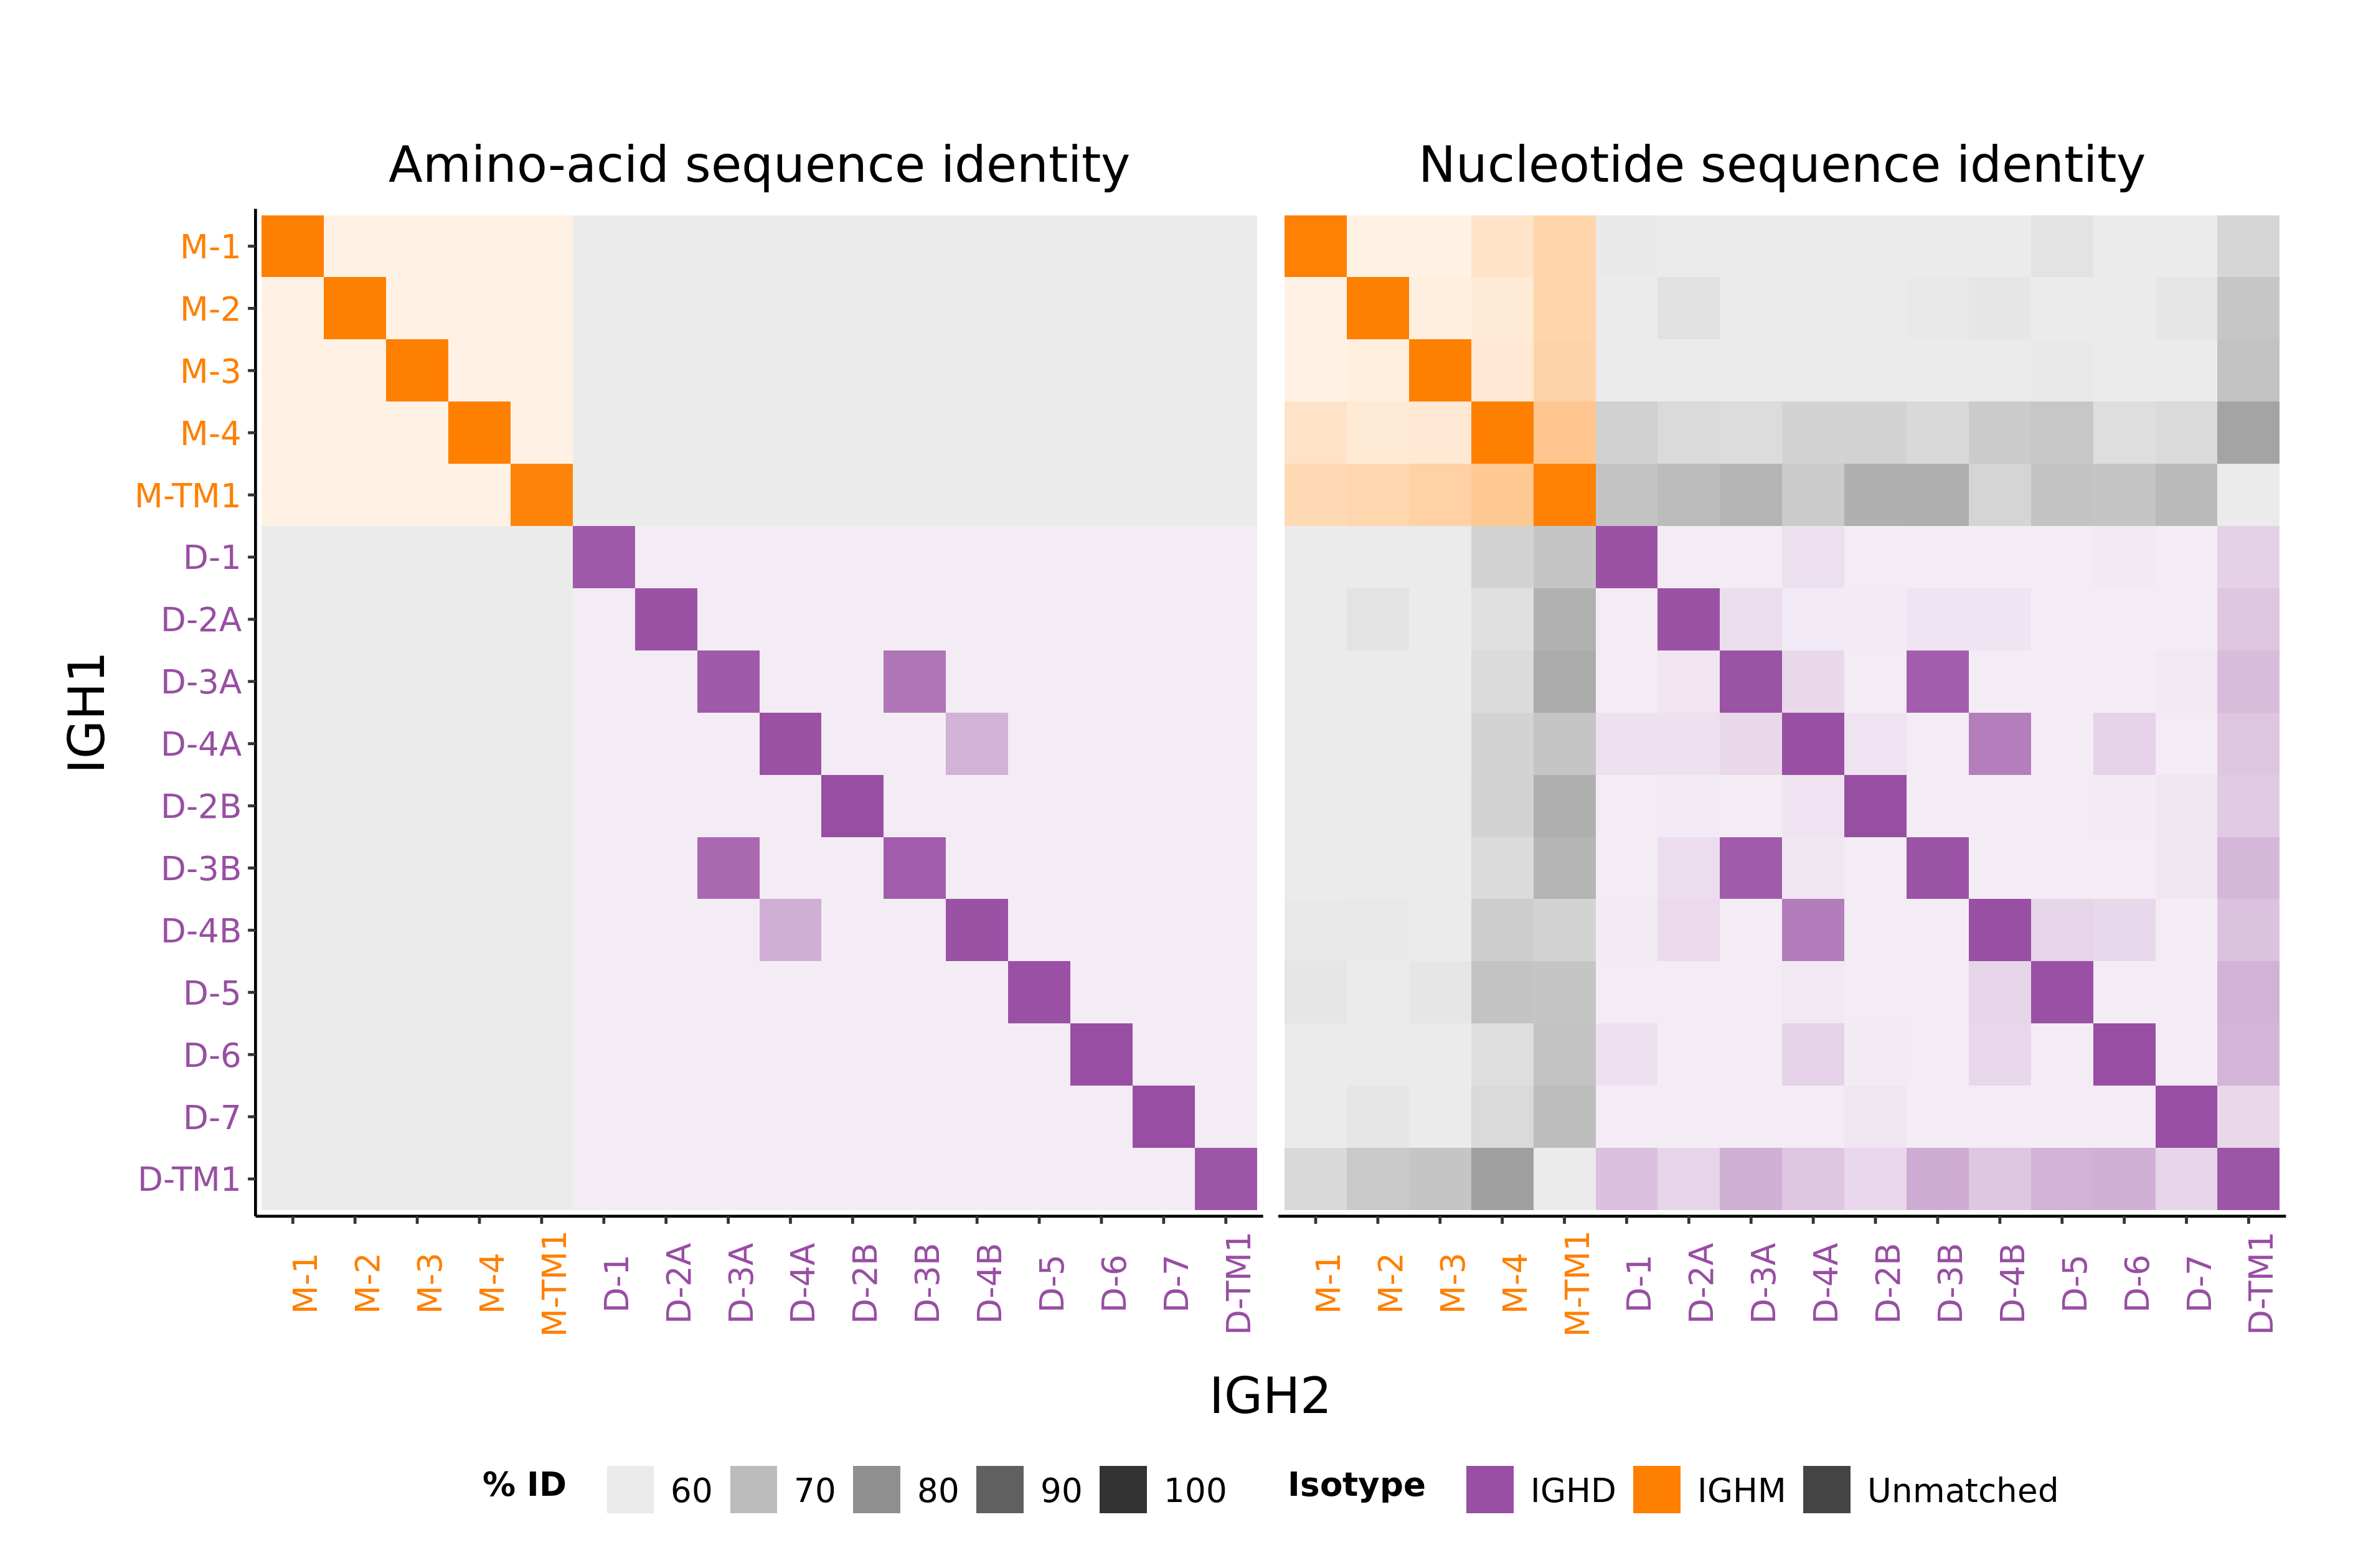
\includegraphics[width = \textwidth]{_Figures/png/nfu-ch-aln}
	\caption[Cross-sublocus sequence similarity in constant-region exons in \Nfu \textit{IGH}]{\textbf{Cross-sublocus sequence similarity in constant-region exons in \Nfu:} Heatmap of percentage sequence identity between amino-acid (right) and nucleotide (left) sequences of constant-region exons (excluding \igh{M-TM2} and \igh{D-TM2}) from the two subloci of \Nfu \textit{IGH}, calculated using pairwise Needleman-Wunsch global alignments..}
	\label{fig:nfu-ch-aln}
	\end{figure}
	
	\begin{table}\centering
		\caption[Cross-sublocus sequence similarity between corresponding constant-region exons in \Nfu \textit{IGH}]{\textbf{Cross-sublocus sequence similarity in constant-region exons in \Nfu:} Percentage sequence identities of pairwise Needleman-Wunsch global alignments between nucleotide (NT) or amino-acid (AA) sequences of corresponding exons from the two subloci of \Nfu \textit{IGH}.}
	% latex table generated in R 3.5.1 by xtable 1.8-3 package
% Wed Dec 19 17:33:43 2018
\begin{tabular}{llrr}
  \toprule Isotype & Exon & NT & AA \\ 
  \midrule M & 1 & 99.66 & 100.00 \\ 
  M & 2 & 100.00 & 100.00 \\ 
  M & 3 & 100.00 & 100.00 \\ 
  M & 4 & 100.00 & 100.00 \\ 
  M & TM1 & 99.34 & 98.00 \\ 
  M & TM2 & 91.67 & 100.00 \\ 
  D & 1 & 99.03 & 97.06 \\ 
  D & 2A & 98.97 & 98.96 \\ 
  D & 3A & 98.72 & 97.09 \\ 
  D & 4A & 99.65 & 98.92 \\ 
  D & 2B & 100.00 & 100.00 \\ 
  D & 3B & 98.72 & 96.12 \\ 
  D & 4B & 99.64 & 98.91 \\ 
  D & 5 & 99.09 & 99.08 \\ 
  D & 6 & 100.00 & 100.00 \\ 
  D & 7 & 100.00 & 100.00 \\ 
  D & TM1 & 97.99 & 97.96 \\ 
  D & TM2 & 99.44 & 100.00 \\ 
   \bottomrule \end{tabular}

	\label{tab:nfu-ch-aln}
	\end{table}
	
\subsection{Variable regions}
\label{sec:nfu-locus-variable}
	
Variable-region gene segments in the killifish \igh{} locus were identified with a variety of methods, depending on the type of gene segment being analysed. \vh candidates were identified probabilistically using Hidden Markov Models constructed by \program{nhmmer} \parencite{wheeler2013nhmmer} from \program{PRANK} \parencite{loytynoja2014prank} multiple-sequence alignments of reference sequences, with the 3'-ends of each V-exon identified by the presence of a recombination-signal sequence (RSS) \parencite{schroeder2010immunoglobulins} and the 5'-ends refined using \program{IMGT-DomainGapAlign} \parencite{ehrenmann2011domaingapalign}. \jh candidates were also identified using \program{nhmmer}, with segment ends identified by the presence of an RSS (5') and a \sequence{GTA} splice-site motif (3') \parencite{magadan2011medaka}. Finally, \dh-segments, being too short and variable in sequence for HMM-based approaches to be effective, were identified by searching for pairs of flanking RSS sequences in opposite orientation, using fuzzy pattern-matching (with EMBOSS \program{FUZZNUC} \parencite{rice2000emboss}) to conserved RSS sequence motifs.
	 
In total, 24 \vh-segments, 14 \dh-segments and 17 \jh-segments were identified in the \Nfu locus (\Cref{tab:nfu-vh-coords,tab:nfu-dh-coords-seg,tab:nfu-jh-coords-seg}), of which the majority (17 \vh, 10 \dh and 8 \jh) were present in \igh{1}. Of the \vh segments identified, three contain premature STOP codons, though none is out-of-frame; conversely, all the \dh and \jh segments identified appear to be in-frame and functional, with no premature STOP codons. However, in all cases a minority of segments contain RSS sequences that deviate significantly from the expected consensus sequence (\Cref{tab:nfu-vh-coords,tab:nfu-dh-coords-rss5,tab:nfu-dh-coords-rss3,tab:nfu-jh-coords-rss}); it is unclear whether these sequences can recombine to successfully produce mature VDJ sequences \textit{in vivo}. In the case of the \vh segments, of the six sequences without clearly functional RSS sequences, three also contain premature STOP codons, suggesting the changes to the RSS in these cases may arise from relaxed purifying selection on already-pseudogenised sequences.

Apart from these few exceptions, however, the recombination signal sequences (RSS) marking the ends of the \vh, \dh and \jh gene segments in the \Nfu locus otherwise strongly resemble those of other characterised teleosts, which in turn resemble those of non-teleost loci (\Cref{fig:nfu-rss-seqlogo-all,fig:nfu-rss-seqlogo-sep}). The overall heptamer and nonamer consensus sequences (\texttt{CACAGTG} for heptamers and \texttt{ACAAAAACC} for nonamers) closely matched those expected from the literature \parencite{schroeder2010immunoglobulins}, while in 88\% of cases the spacer region was within 1bp of the expected length (12bp for D-RSSs, 23bp for V- and J-RSSs); unexpectedly, the greatest number of \vh-RSSs had a 22bp (rather than 23bp) spacer, but this is unlikely to interfere with RSS functionality. Overall, the RSSs in the turquoise killifish appear to be supporting the normal operation of VDJ-recombination in this species.

Of the \vh, \dh and \jh segments identified, all but one of each type of segment is located within contiguous V-, D-, and J-regions within each sublocus, supporting a modified translocon configuration for killifish \igh. The exceptions to this are \igh{1D01} and \igh{1J01}, which are embedded within the \igh{1} V-region, and a single \vh segment located in between the \igh{D} contant regions of the two subloci (\Cref{fig:nfu-locus-map-b}). The unusual location of \igh{1D01} and \igh{1J01} may represent the result of a transposition event within the \igh{} locus; however, their close colocalisation and 5' position within the \igh{1} sublocus, as well as the fact that neither has a close paralogue in \igh{2} (\Cref{fig:nfu-dj-alignment-b}), suggest that they may instead represent the remnant of a formerly present \igh{Z} constant region, as these typically have dedicated D/J segments independent of those serving \igh{M}. Given its forward orientation, meanwhile, the orphaned \vh-segment was assigned to the \igh{1} sublocus as \igh{1V1-07}; however, if annotated correctly, it is unlikely to successfully recombine with segments in either sublocus due to its unusual location.
		
\begin{table}[hb]
	\centering
	\begin{threeparttable}
	\centering
	\caption{Number of functional \vh-segments and \vh-families in other teleost species.}
	\label{tab:teleost-vh-counts}
	\begin{tabular}{ccccc}\toprule
	\multirow{2}{*}{	\textbf{Common Name}} & \multirow{2}{*}{\textbf{Species}} & \textbf{\# Functional} & \textbf{	\# \vh} & \multirow{2}{*}{\textbf{Source}} \\
	& & \textbf{\vh Segments} & \textbf{Families} & \\\midrule
	Zebrafish & \textit{Danio rerio} & 39 & 13\,\tnote{1} & \parencite{magadan2015fishrepertoires} \\
	Grasscarp & \textit{Ctenopharyngodon idella} & 8 & 5\,\tnote{2} & \parencite{xiao2010grasscarp} \\
	Fugu & \textit{Takifugu rubripes} & 34 & 3 & \parencite{magadan2015fishrepertoires} \\
	Medaka & \textit{Oryzias latipes} & 35 & 6 & \parencite{fillatreau2013astonishing,magadan2011medaka} \\
	Stickleback & \textit{Gasterosteus aculeatus} & 49 & 4 & \parencite{magadan2015fishrepertoires} \\
	Turquoise killifish & \textit{Nothobranchius furzeri} & 21\,\tnote{3} & 6 & -- \\
	\bottomrule\end{tabular}
	\begin{tablenotes}
	\item[1] \vh families in zebrafish identified based on 70\% (rather than 80\%) sequence identity.
	\item[2] It is not clear what clustering method or threshold was used to identify \vh families in grasscarp.
	\item[3] Excluding \vh segments with nonsense or frameshift mutations, but not those with uncertain or missing RSS sequences.
	\end{tablenotes}
	\end{threeparttable}
\end{table}
	
\vh sequences within an \igh{} locus are conventionally grouped into families on the basis of nucleotide sequence identity, with a typical identity cutoff of 80\% \parencite{magadan2015fishrepertoires}. In order to group the \Nfu \vh genes into families, pairwise Needleman-Wunsch global alignments were performed on each pair of \vh sequences to obtain pairwise identity scores, followed by single-linkage clustering on the resulting identity matrix. Cutting the dendrogram at 80\% sequence identity revealed a total of six \vh families, of which four contained more than one \vh segment (\Cref{fig:nfu-vh-families}); this number of \vh families in the \Nfu locus is roughly in line with those found in related species (\Cref{tab:teleost-vh-counts}). Of these, V1 and V2 make up the bulk (42\% and 29\% respectively) of the \vh segments in the locus. V2 and V4 are highly similar, and all the members of V4 are pseudogenised by premature STOP codons; it may therefore be more appropriate to regard V4 as a pseudogenised subfamily of V2 than as a \vh family in its own right.

The total number of functional \vh segments in the killifish locus is unusually small in comparison to the total numbers observed in many other teleost species (\Cref{tab:teleost-vh-counts}); however, the number of segments per sublocus is in line with the numbers seen in closely-related species (2 to 12 in medaka, 6 to 18 in stickleback), with the overall difference mainly arising from a difference in the number of subloci per locus. A similar pattern is observed with \dh and \jh segments, with similar numbers of segments per sublocus in killifish and closely-related species, especially medaka. It therefore appears that the per-sublocus segment diversity available to the turquoise killifish is similar to that of previously characterised species, with any difference in total available diversity at this level arising from differences in the number of functional subloci rather than the size of the V/D/J-regions \textit{per se}.

As can be seen from \Cref{fig:nfu-locus-synteny}, much of the V-, D- and especially J-region sequence in the \Nfu locus is syntenic between the two \igh{} subloci, with downstream portions of the \igh{2} V-region corresponding to downstream parts of the \igh{1} region. Of the seven \vh segments in \igh{2}, six have a correspending segment on \igh{1} with which they share at least 97\% sequence identity (\Cref{fig:nfu-vh-families}), and these partner segments are largely (though not entirely) colinear in their ordering between the two subloci. A similar pattern can be observed for the D- and (especially) the J-regions: of the four \dh segments detectable in \igh{2}, three (\igh{2D02} to \igh{2D04}) are identical with another block of adjacent \dh segments in \igh{1} (\igh{1D05} to \igh{1D07}), while the \jh-regions exhibit almost complete sequence identity between the eight \jh segments of the main \jh region in \igh{1} and the eight \jh segments in \igh{2} (\Cref{fig:nfu-dj-alignment}).
		
Nevertheless, as is clear from \Cref{fig:nfu-locus-synteny}, there are large portions the \igh{1} variable region, including the first 25 kilobases of the V-region, for which no corresponding sequence exists in \textit{IGH2}, and there are many \vh and \dh segments in \igh{1} (and a much smaller number in \igh{2}) for which no close homologue exists in the other sublocus. Taken together, these data are consistent with a model in which \igh{2} was produced via duplication and inversion of all or part of \igh{1}, followed by subsequent deletion events in the redundant, and structurally volatile, \igh{2} \vh and \dh regions. However, it is not clear at present how to distinguish between this model and an alternative one of expansion in \igh{1}, or to identify why the \jh region is so much more conserved between subloci than either the \vh or \jh regions.

	
	\begin{figure}
	\centering
	\begin{subfigure}{0em}
	\phantomsubcaption{}
    \label{fig:nfu-vh-families-a}
    \end{subfigure}
    \begin{subfigure}{0em}
    \phantomsubcaption{}
    \label{fig:nfu-vh-families-b}
    \end{subfigure}
	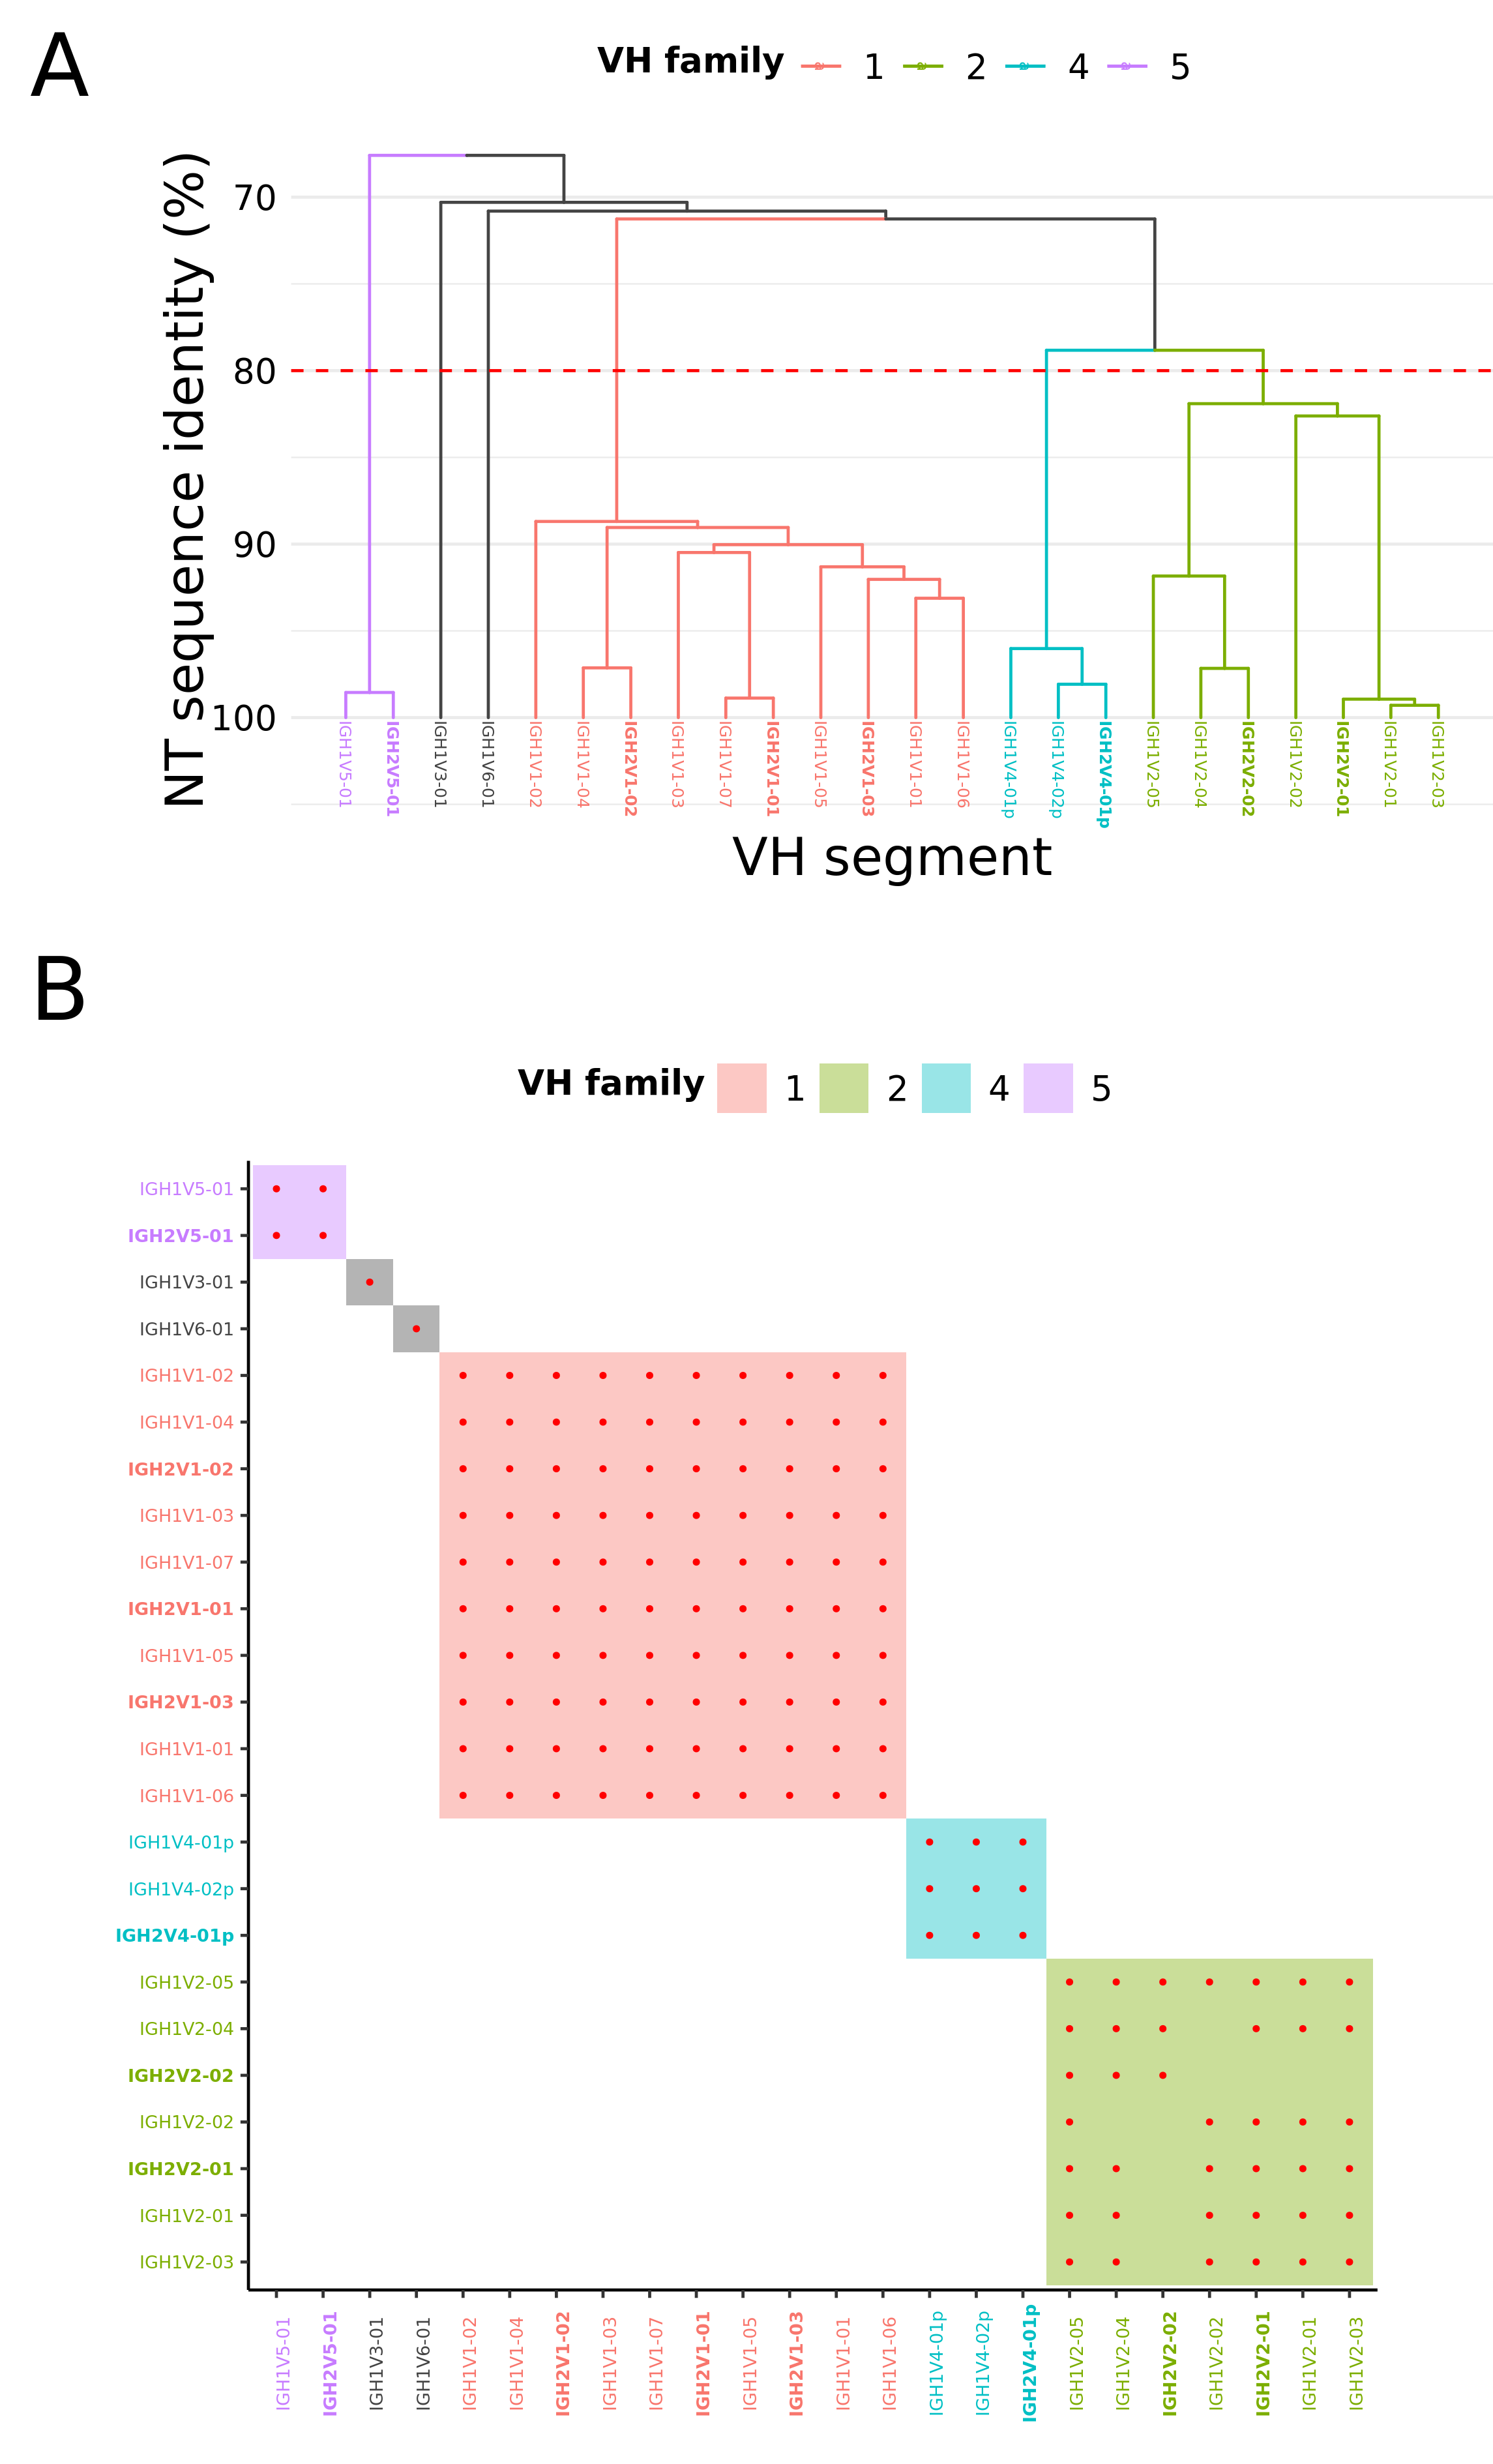
\includegraphics[width=0.8\textwidth]{_Figures/png/nfu-vh-families.png}
	\caption[\vh families in the in \Nfu \igh{} locus]{\textbf{\vh families in the in \Nfu \igh{} locus:} (A) Dendrogram of sequence similarity of \vh segments in the \Nfu \igh{} locus, arranged by single-linkage clustering on nucleotide sequence identity. The red line indicates the 80\% cutoff point for family assignment, while branch colour indicates family membership. (B) Heatmap of family relationships among \Nfu \vh segments, with coloured shading indicating families and red dots indicating pairwise nucleotide sequence identity of at least 80\%. In both subfigures, \vh families containing multiple segments are coloured, single-segment families are in grey, and segments from the \igh{2} sublocus are displayed in \textbf{boldface}.}
	\label{fig:nfu-vh-families}
	\end{figure}

\begin{figure}
\centering
	\centering
	\begin{subfigure}{0em}
	\phantomsubcaption{}
    \label{fig:nfu-dj-alignment-a}
    \end{subfigure}
    \begin{subfigure}{0em}
    \phantomsubcaption{}
    \label{fig:nfu-dj-alignment-b}
    \end{subfigure}

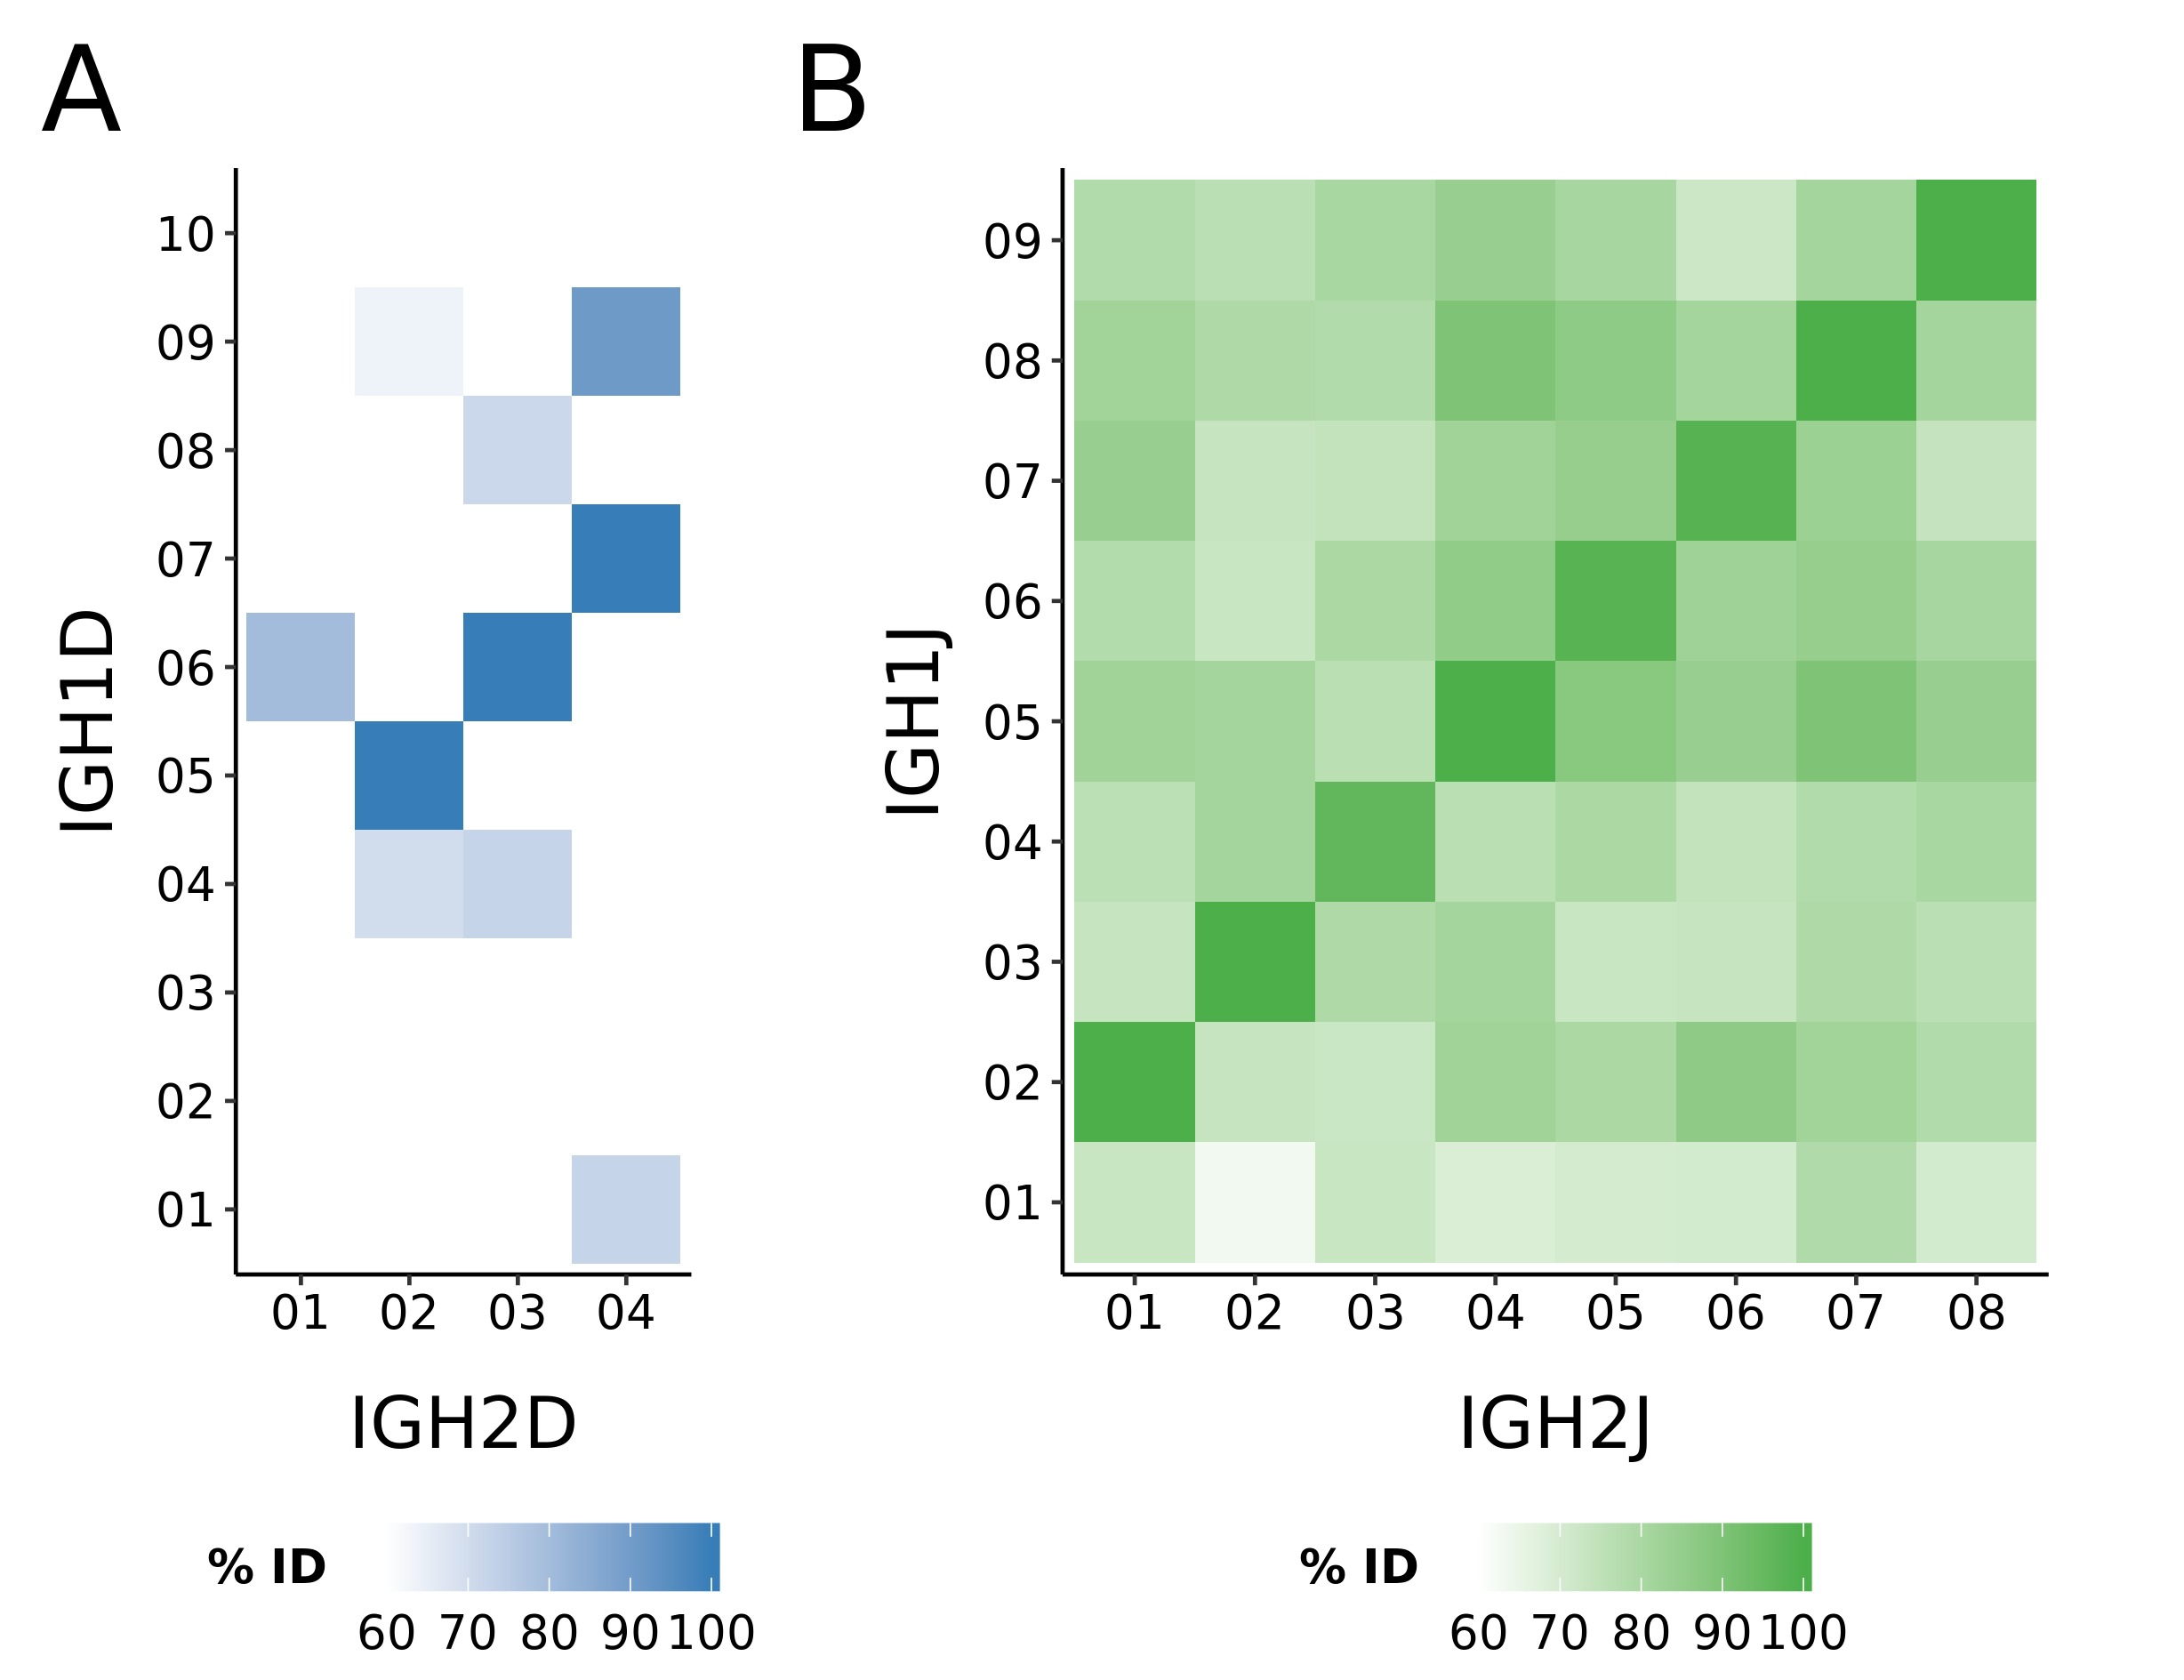
\includegraphics[width=0.6\textwidth]{_Figures/png/nfu-dj-aln}
\caption[Cross-sublocus sequence similarity in \dh and \jh gene segments in \Nfu]{\textbf{Cross-sublocus sequence similarity in \dh and \jh gene segments in \Nfu:} Heatmap of percentage nucleotide sequence identities of Needleman-Wunsch global alignments between (A) \dh and (B) \jh gene segments in IGH1 vs IGH2, revealing syntenic runs of highly similar sequences across both subloci.}
\label{fig:nfu-dj-alignment}
\end{figure}	
	
	\begin{figure}
	\centering
	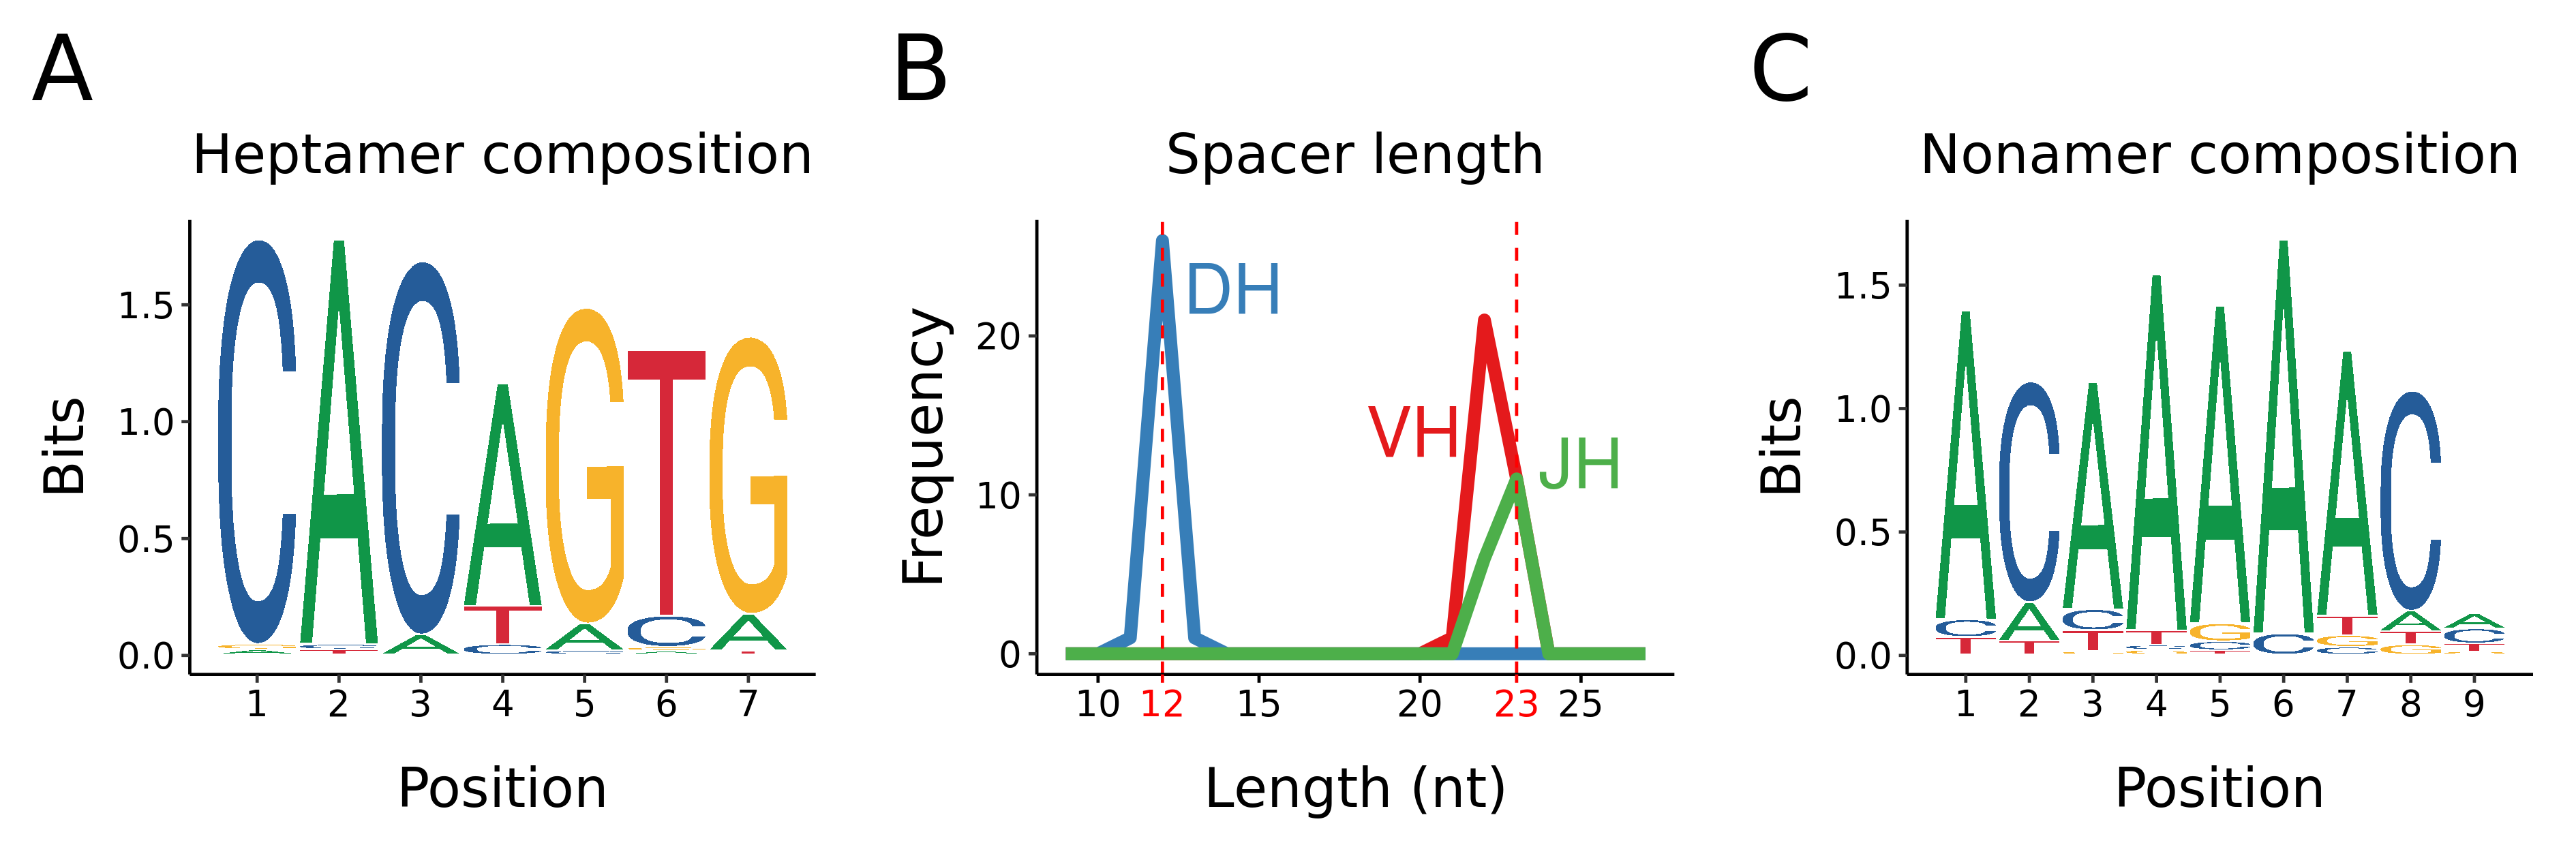
\includegraphics[width=\textwidth]{_Figures/png/nfu-rss-seqlogo-all}
	\caption[Recombination signal sequences in the \Nfu \textit{IGH} locus]{\textbf{Recombination signal sequences in the \Nfu \textit{IGH} locus:} (A) Sequence composition of conserved heptamer sequences across all \Nfu heavy-chain RSSs; (B) length distribution of unconserved spacer sequences in \Nfu heavy-chain RSSs; (C) sequence composition of conserved heptamer sequences across all \Nfu heavy-chain RSSs.}
	\label{fig:nfu-rss-seqlogo-all}
	\end{figure}
	
\FloatBarrier



\clearpage

%%%%%%%%%%%%%%%%%%%%%%%%%%%%%%%%%%%%%%%%%%%%%%%%%%%%%%%%%%%%%%%%%%%%%%%%%%%%%%%
% KILLIFISH LOCUS SECTION
%%%%%%%%%%%%%%%%%%%%%%%%%%%%%%%%%%%%%%%%%%%%%%%%%%%%%%%%%%%%%%%%%%%%%%%%%%%%%%%

\section{The \igh{} locus in \xma}
\label{sec:xma-locus}
	
	The turquoise killifish \igh{} locus shares many features with other characterised teleost loci, including a modified tandem-translocon configuration with intact \vh, \dh, \jh and constant regions (\Cref{fig:nfu-locus-map-b}), a four-exon secreted configuration of \igh{M} (\Cref{fig:nfu-locus-sashimi-a}), an expanded \igh{D} constant region with tandem \cd{}-exon block repeats (\Cref{fig:nfu-locus-sashimi-b,fig:nfu-locus-map-b},), a conserved RSS structure (\Cref{fig:nfu-rss-seqlogo-all}), and a chimeric \cm{1} in \igh{D} (\Cref{fig:nfu-locus-sashimi-b}). However, it also exhibits many ideosyncratic features that differ from those observed in most characterised teleost loci, including an unusually small number of \vh segments (\Cref{fig:nfu-vh-families} and \Cref{tab:teleost-vh-counts}), a four-exon \cm{1}-\cm{2}-TM1-TM2 configuration of transmembrane \igh{M} (\Cref{fig:nfu-locus-sashimi-a}), an inverted sublocus present in antisense (\Cref{fig:nfu-locus-map-b}), and a complete absence of \igh{Z}.
	
Many of these peculiarities, including the unusual \igh{M-TM} splicing pattern, inverted sublocus, and lack of \igh{Z}, are shared with the \igh{} locus of medaka (\textit{Oryzias latipes}), which is the closest relative of \textit{Nothobranchius furzeri} to have its immunoglobulin heavy chain locus characterised prior to this study \parencite{magadan2011medaka}. Given the close relationship between the two species, the shared unusual features of their \igh{} loci suggested a common origin of these traits  in the common ancestor of both species. If this hypothesis were correct, one would expect \igh{Z} to also be absent in any other descendents of this common ancestor, including other cyprinodontiform species.

To investigate this hypothesis further, I performed a complete characterisation of the \igh{} locus in the platyfish \textit{Xiphophorus maculatus}, another cyprinodontiform species that has seen widespread use as a model organism \parencite{schartl2013platyfish}. Surprisingly, the \Xma locus shared none of the unusual features shared between the turquoise-killifish and medaka loci, strongly suggesting independent loss of \igh{Z} in both groups and implying a high level of volatility in \igh{} locus structure within the Atherinomorpha.

\subsection{Overall structure}
\label{sec:xma-locus-structure}
	
As was the case with the \Nfu \igh{} locus, candidate genome scaffolds from the most recent \xma genome assembly (Genbank accession GCA\_002775205.2) were identified by alignment to \igh{} gene segments from zebrafish, stickleback and medaka, supplemented in this case with segments from the newly-characterised \Nfu locus itself. In contrast to the more fragmented results in \Nfu, this process identified a single sequence region on one chromosome of the \Xma locus, which was extracted and characterised as described for the assembled \Nfu locus (\Cref{sec:nfu-locus}) without the need for further sequencing or assembly.

The \Xma \igh{} locus so identified occupies roughly \kb{293} on chromosome 16 (scaffold NC\_036458.1; \Cref{fig:xma-locus-map-a}). Unlike in turquoise killifish and medaka, all identified gene segments share a common orientation; no evidence of a second sublocus in antisense could be identified. In stark contrast with both killifish and medaka, the single ``sublocus" comprising \Xma \igh{} contains not one but two \igh{Z} constant regions, along with a hugely extended V-region extending over almost \kb{250} and containing more than 120 \vh-segments. This enormous \vh-diversity greatly exceeds that of any characterised teleost \igh{} locus except perhaps that of rainbow trout \parencite{bengten2015fishantibodies}, while the presence of multiple \igh{Z} constant regions without intervening \igh{M} or \igh{D} is also highly unusual \parencite{fillatreau2013astonishing}. 

Even cursory examination of the \Xma \igh{} locus is therefore sufficient to reveal a unique and highly interesting structure with many unexpected differences from both turquoise killifish and medaka (\Cref{fig:species-tree-small}, columns 1-5). In particular, since \Xma is more closely related to \Nfu than either is to medaka, the presence of \igh{Z} in the former strongly suggests at least two independent loss events in the Atherinomorpha, indicating an unexpected level of volatility in the evolution of this important isotype.
 
	\begin{figure}
	\centering
	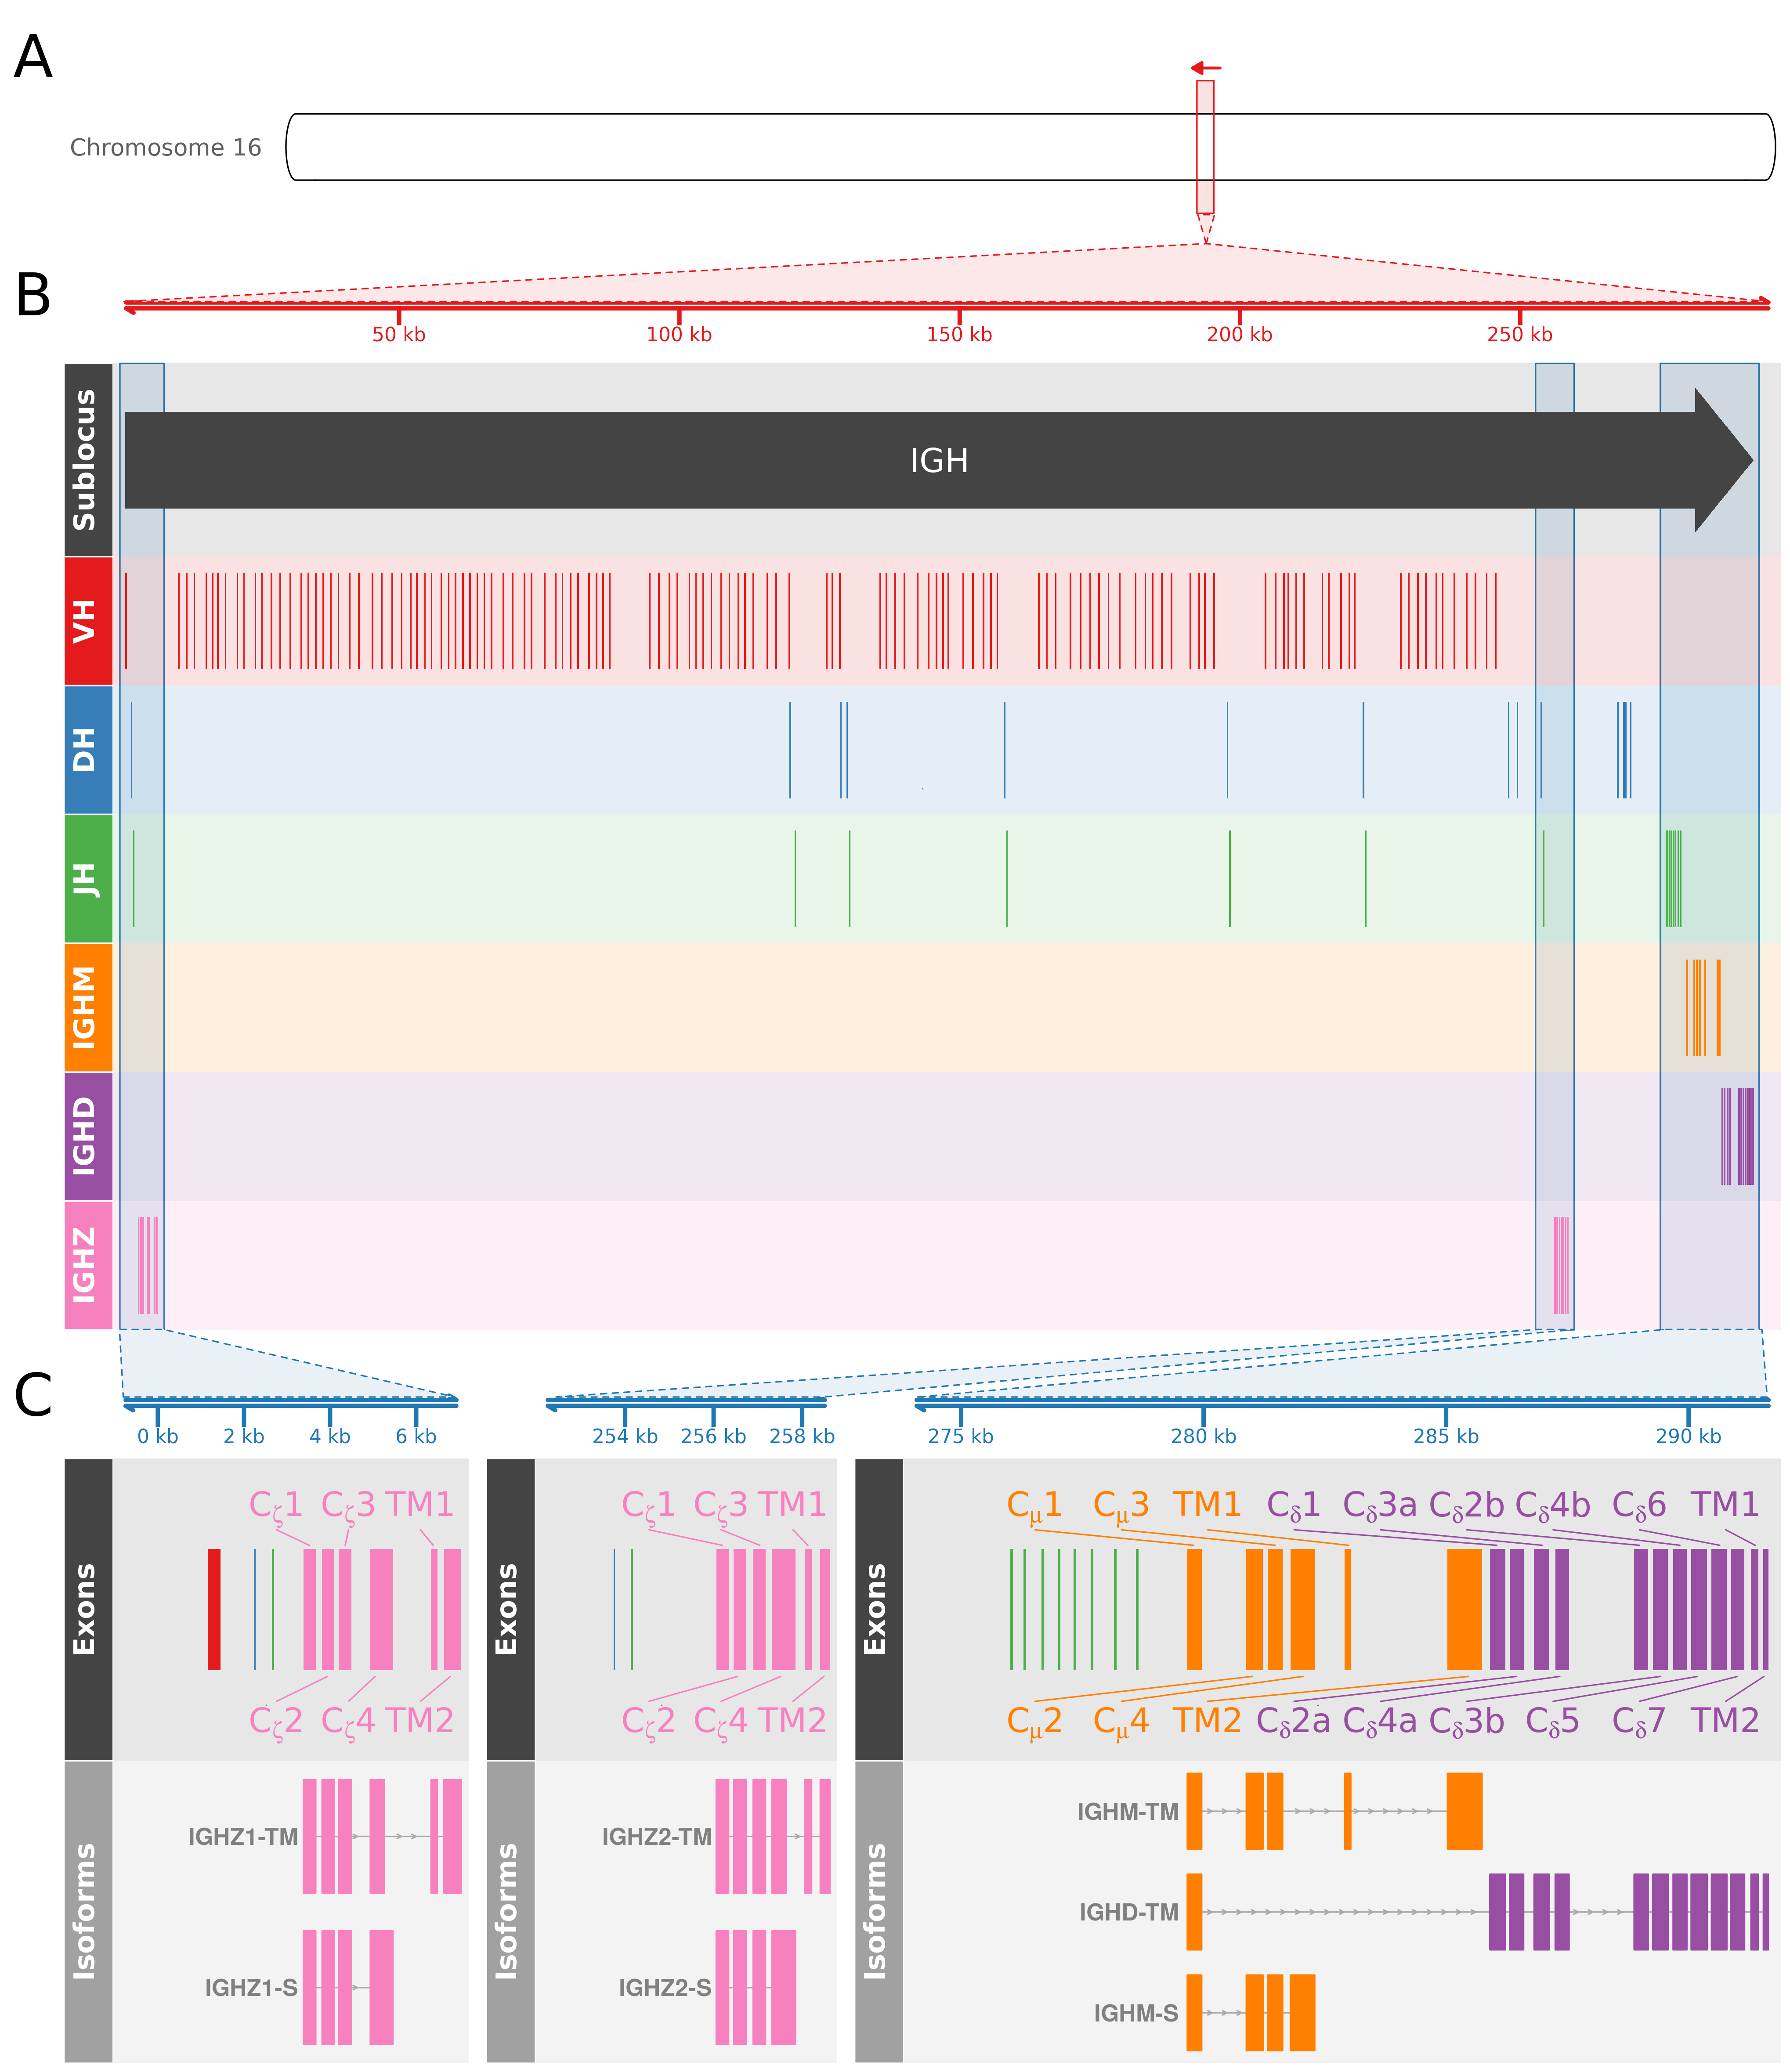
\includegraphics[width=\textwidth]{_Figures/png/xma-new-locus-map}
	\caption[The immunoglobulin heavy chain (\textit{IGH}) locus in \textit{}]{\textbf{The immunoglobulin heavy chain (\textit{IGH}) locus in \textit{Xiphophorus maculatus}:} (A) Position of the \textit{IGH} locus on chromosome (group) 16 of the \Xma genome. (B) Arrangement of \vh, \dh, \jh and constant-region gene segments on the \Xma \igh{} locus. (C) Detailed map of the \igh{Z1}, \igh{Z2} and \igh{M/D} constant regions, indicating the position and identity of the constant-region exons and the exon composition of expressed \igh{} isoforms in \Xma. Note change of orientation between subfigures (A) and (B-C).}
	\begin{subfigure}{0em}
        \phantomsubcaption{}
        \label{fig:xma-locus-map-a}
    \end{subfigure}
    \begin{subfigure}{0em}
        \phantomsubcaption{}
        \label{fig:xma-locus-map-b}
    \end{subfigure}
    \begin{subfigure}{0em}
        \phantomsubcaption{}
        \label{fig:xma-locus-map-c}
    \end{subfigure}
	\label{fig:xma-locus-map}
\end{figure} % TODO: Fix to remove IGHZ2-S

\begin{figure}
\centering
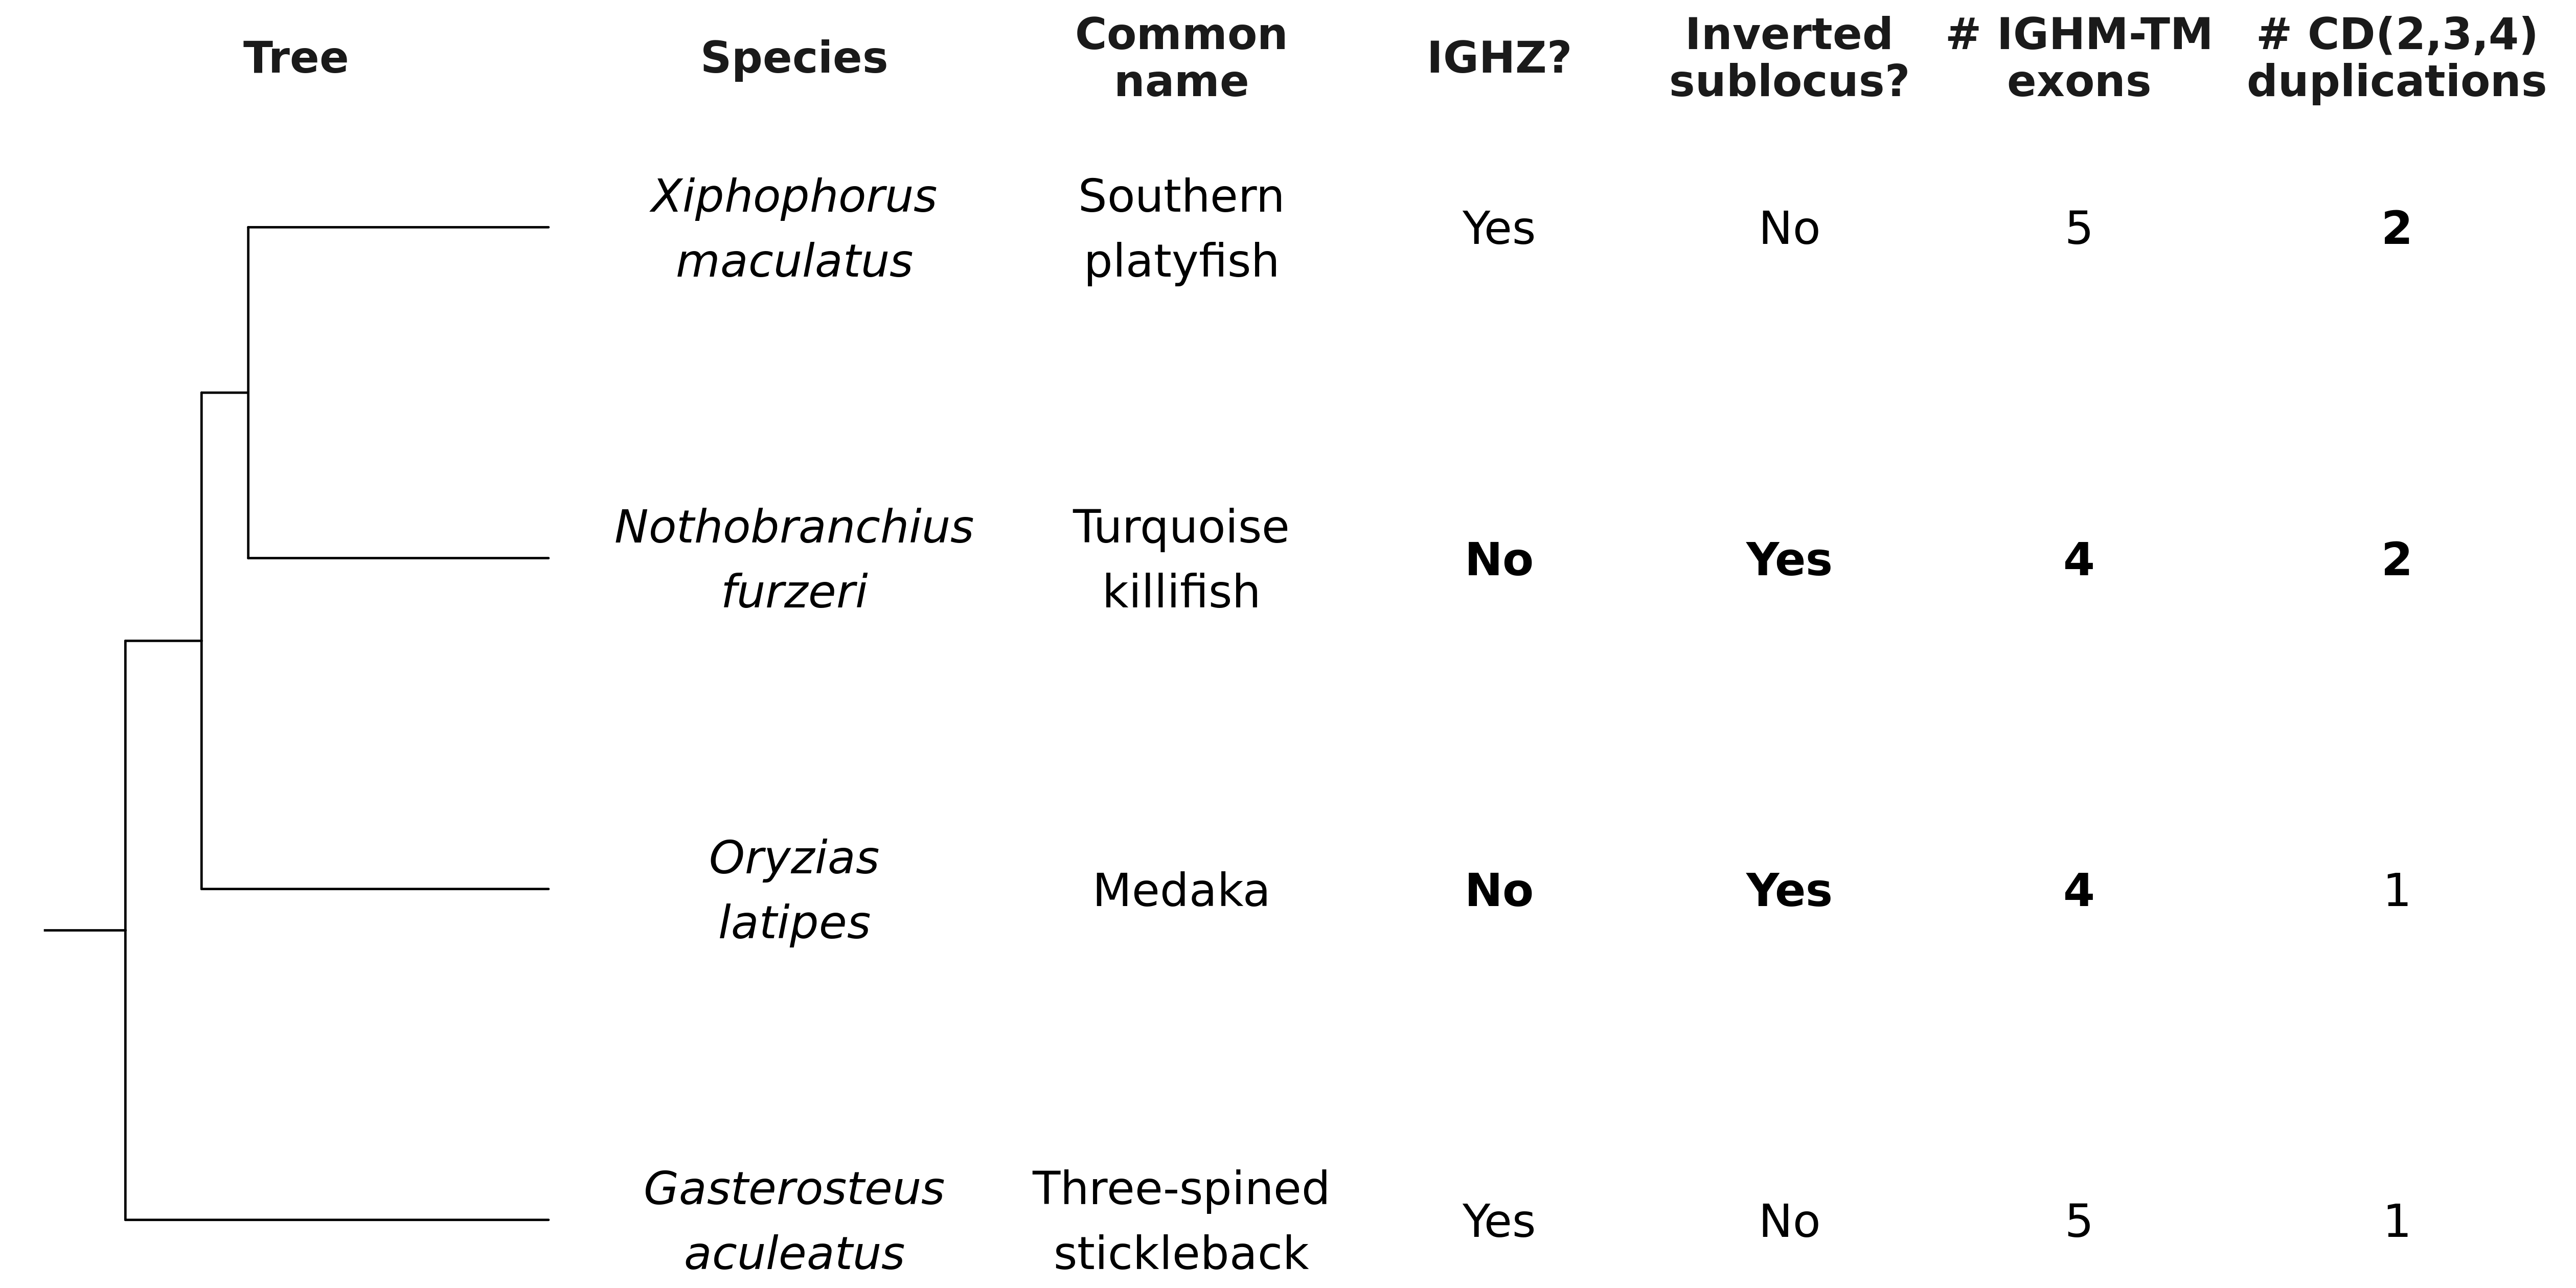
\includegraphics[width=\textwidth]{_Figures/png/species-tree-small}
\vspace{0.5em}
\caption[Summary of important \igh{} phenotypes in killifish, platyfish, and medaka]{\textbf{Summary of important \igh{} phenotypes in killifish, platyfish, and medaka:} Cladogram of the evolutionary relationship between southern platyfish (\xma), turquoise killifish (\nfu) and medaka (\species{Oryzias}{latipes}), with three-spined stickleback (\species{Gasterosteus}{aculeatus}) as an outgroup. The state of various \igh{} phenotypes of interest are annotated to the right of the tree; states deviating from the expected teleost configuration are in bold.}
\label{fig:species-tree-small}
\end{figure}
	
\subsection{Constant regions}
\label{sec:xma-locus-constant}
	
As discussed briefly in \Cref{sec:xma-locus-structure}, the \Xma \igh{} locus contains two distinct \igh{Z} constant regions: one in the usual position immediately preceding the \igh{M}-associated D- and J-regions, the other, unexpectedly, at the far 5'-extremity of the locus (\Cref{fig:xma-locus-map-b}). Both \igh{Z} constant regions occupy the expected configuration, with four \cz{} exons, two transmembrane exons, and a secretory tail (\Cref{fig:xma-locus-map-c}, \Cref{tab:xma-ch-coords}). However, in contrast to the duplicate constant regions in \Nfu, the two \igh{Z} constant regions in \Xma are quite distinct from each other in sequence, with an average of only \pc{64} nucleotide and \pc{48} amino-acid sequence identity between corresponding \cz{} exons (\Cref{fig:xma-cz-aln}, \Cref{tab:xma-cz-aln}). This unexpectedly high level of sequence divergence suggests a relatively ancient duplication event, and raises the possibility that the lineage giving rise to \Nfu may have lost not one, but two distinct \igh{Z} constant regions.
	
\begin{figure}
	\centering
	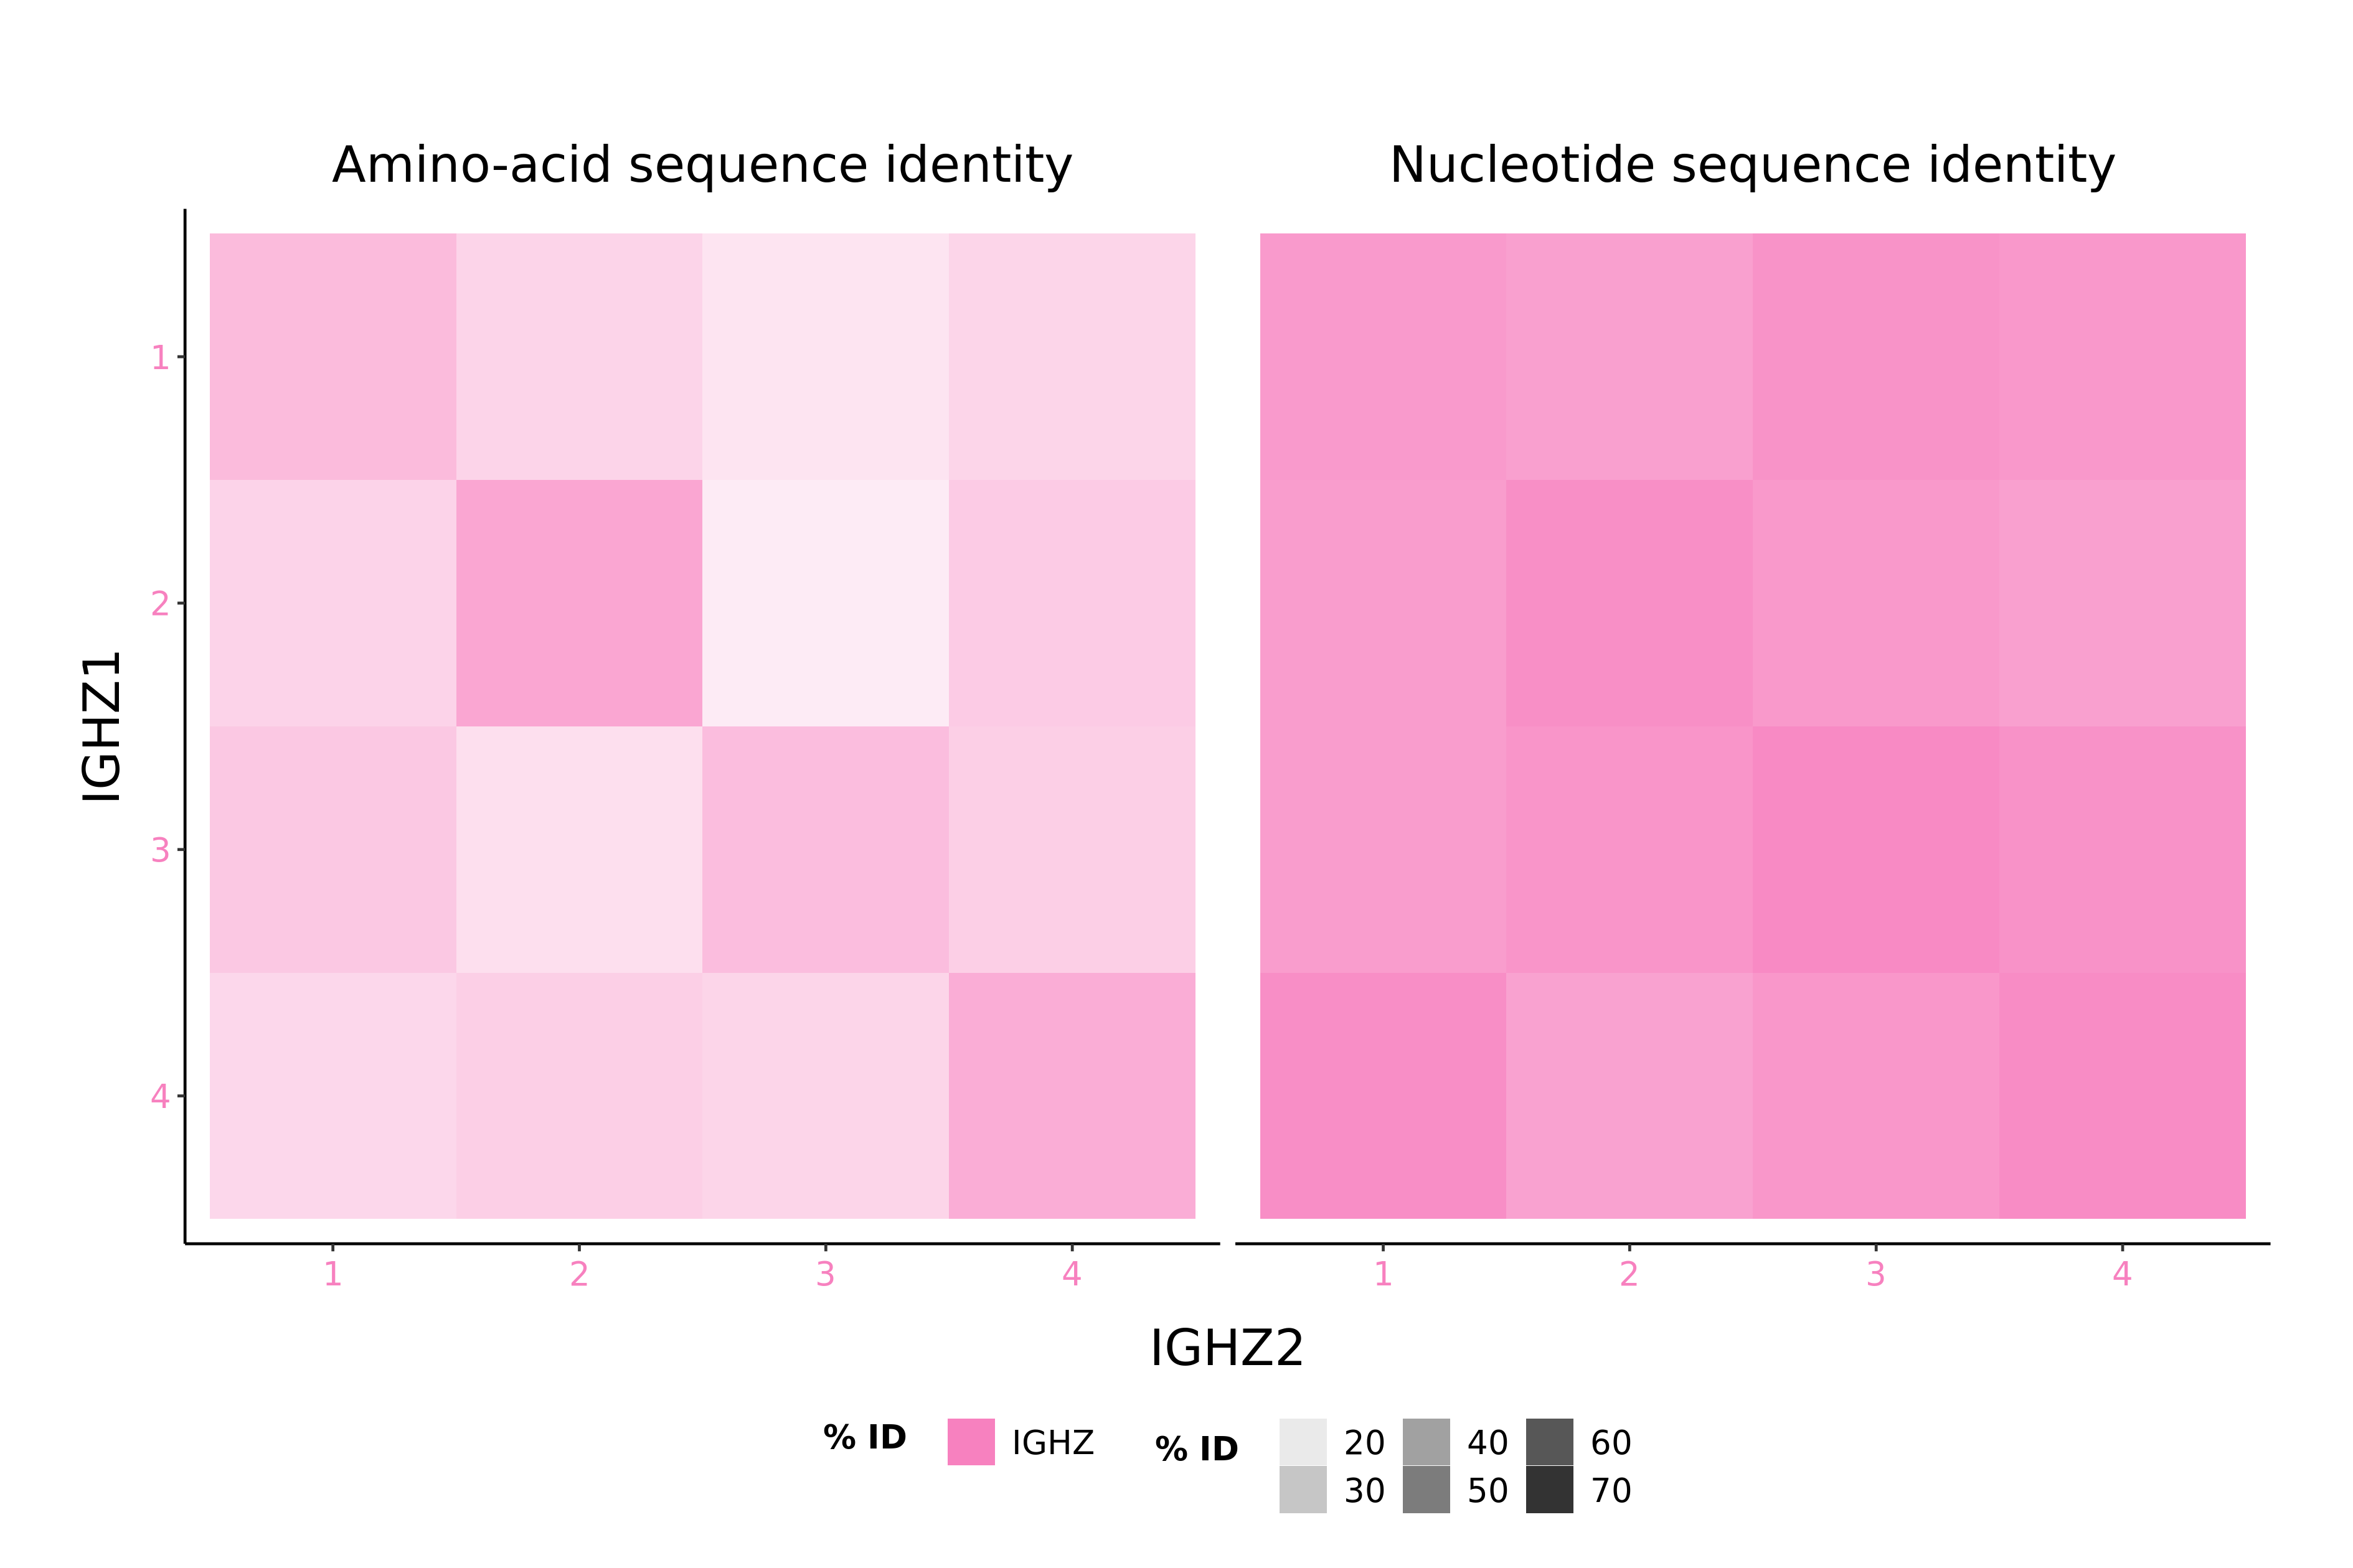
\includegraphics[width=0.8\textwidth]{_Figures/png/xma-new-cz-aln}
	\caption[Sequence similarity between \igh{Z} constant-regions in \Xma]{\textbf{Sequence similarity between \igh{Z} constant-regions in \Xma:} Heatmap of percentage sequence identity between amino-acid (right) and nucleotide (left) sequences of \cz{} exons from the two \Xma \igh{Z} constant regions, calculated using pairwise Needleman-Wunsch global alignments.} % TODO: Combine isotype and identity legends
	\label{fig:xma-cz-aln}
\end{figure}

\begin{table}
	\centering
	\caption[Sequence similarity between \igh{Z} constant-regions in \Xma]{\textbf{Sequence similarity between \igh{Z} constant-regions in \Xma:} Percentage sequence identities of pairwise Needleman-Wunsch global alignments between nucleotide (NT) or amino-acid (AA) sequences of corresponding \cz{} exons from the two \igh{Z} constant regions of \Xma \textit{IGH}.}
	% latex table generated in R 3.5.2 by xtable 1.8-3 package
% Tue Jan  8 14:15:22 2019
\begin{tabular}{llrr}
  \toprule Isotype & Exon & NT & AA \\ 
  \midrule Z & 1 & 59.14 & 44.57 \\ 
  Z & 2 & 63.93 & 53.41 \\ 
  Z & 3 & 66.19 & 43.48 \\ 
  Z & 4 & 65.15 & 50.49 \\ 
   \bottomrule \end{tabular}

	\label{tab:xma-cz-aln}
\end{table}

\begin{table}\centering
    \caption{Co-ordinate table of constant-region exons in the \xma \igh{} locus.}
    	% latex table generated in R 3.5.2 by xtable 1.8-3 package
% Tue Jan  8 15:33:35 2019
\begin{tabular}{llrrrl}
  \toprule Name & Isotype & Start & End & Length & Strand \\ 
  \midrule IGHZ1-1 & Z & 3380 & 3667 & 288 & + \\ 
  IGHZ1-2 & Z & 3814 & 4098 & 285 & + \\ 
  IGHZ1-3 & Z & 4195 & 4497 & 303 & + \\ 
  IGHZ1-4 & Z & 4934 & 5263 & 330 & + \\ 
  IGHZ1-S & Z & 5264 & 5459 & 196 & + \\ 
  IGHZ1-TM1 & Z & 6345 & 6490 & 146 & + \\ 
  IGHZ1-TM2 & Z & 6645 & 7043 & 399 & + \\ 
  IGHZ2-1 & Z & 256059 & 256337 & 279 & + \\ 
  IGHZ2-2 & Z & 256453 & 256734 & 282 & + \\ 
  IGHZ2-3 & Z & 256893 & 257171 & 279 & + \\ 
  IGHZ2-4 & Z & 257319 & 257636 & 318 & + \\ 
  IGHZ2-S & Z & 257637 & 257850 & 214 & + \\ 
  IGHZ2-TM1 & Z & 258059 & 258213 & 155 & + \\ 
  IGHZ2-TM2 & Z & 258410 & 258629 & 220 & + \\ 
  IGHM-1 & M & 279664 & 279960 & 297 & + \\ 
  IGHM-2 & M & 280880 & 281224 & 345 & + \\ 
  IGHM-3 & M & 281321 & 281629 & 309 & + \\ 
  IGHM-4 & M & 281789 & 282291 & 503 & + \\ 
  IGHM-TM1 & M & 282910 & 283034 & 125 & + \\ 
  IGHM-TM2 & M & 285028 & 285740 & 713 & + \\ 
  IGHD-1 & D & 285902 & 286219 & 318 & + \\ 
  IGHD-2A & D & 286310 & 286597 & 288 & + \\ 
  IGHD-3A & D & 286814 & 287128 & 315 & + \\ 
  IGHD-4A & D & 287250 & 287534 & 285 & + \\ 
  IGHD-2B & D & 288876 & 289166 & 291 & + \\ 
  IGHD-3B & D & 289262 & 289576 & 315 & + \\ 
  IGHD-4B & D & 289680 & 289964 & 285 & + \\ 
  IGHD-5 & D & 290052 & 290381 & 330 & + \\ 
  IGHD-6 & D & 290472 & 290789 & 318 & + \\ 
  IGHD-7 & D & 290865 & 291152 & 288 & + \\ 
  IGHD-TM1 & D & 291286 & 291434 & 149 & + \\ 
  IGHD-TM2 & D & 291541 & 291642 & 102 & + \\ 
   \bottomrule \end{tabular}

    \label{tab:xma-ch-coords}
\end{table}

While the state of \igh{Z} constant regions differs markedly between \Xma and \Nfu, the configurations of the \igh{M} and \igh{D} constant regions of the two species are quite similar, with a {\cm{1}-\cm{2}-\cm{3}-\cm{4}-TM1-TM2} configuration for \igh{M} and a {\cd{1}-(\cd{2}-\cd{3}-\cd{4})$_2$-\cd{5}-\cd{6}-\cd{7}-TM1-TM2} configuration for \igh{D} (\Cref{fig:xma-locus-map-b,fig:xma-locus-map-c}, \Cref{tab:xma-ch-coords}). In the \Xma locus, these constant regions and \igh{Z1} adopt the standard configuration seen in comparatively simple teleost \igh{} loci like those of zebrafish and fugu, with a {\vh-\dh-\jh-\textbf{CZ}-\dh-\jh-\textbaf{CM}-\textbf{CD}} arrangement that allows the choice between \igh{Z} and \igh{M/D} usage to be made via the choice of \dh segment during VDJ-recombination. However, whether such a mechanism is also responsible for the choice between these constant regions and \igh{Z1}, which lies more than \kb{200} away and upstream of the great majority of \vh segments in the locus (\Cref{sec:xma-locus-variable}) is questionable.

In order to investigate the expressed isoforms present in \Xma, published RNA-sequencing reads from various platyfish tissues (BioProject accession PRJNA420092, all libraries). were aligned together to the \igh{Z} and \igh{M/D} constant regions with \program{STAR}. The results indicate the expected six-exon transmembrane configuration in both \igh{Z1} and \igh{Z2}, as well as a secretory form of \igh{Z1} comprising \cz{1} to \cz{4} plus a \bp{23} secretory tail formed by a transcriptional run-on event from \cz{4} (\Cref{fig:xma-locus-sashimi-z1,fig:xma-locus-sashimi-z2}). However, while an in-frame secretory tail of similar length (\bp{20}) can be found in \igh{Z2}, it does not appear to be expressed in the read sets analysed here, indicating that \igh{Z2} may only be expressed in transmembrane form in the individuals sampled (\Cref{fig:xma-locus-sashimi-z2}).

Meanwhile, the results for \igh{D} (\Cref{fig:xma-locus-sashimi-d}) indicate a similar configuration to that observed in turquoise killifish, with a chimeric \cm{1} followed by 10 \cd{} exons and two transmembrane exons; as in \Nfu, neither a dedicated \igh{D} secretory exon nor a post-\cd{7} secretory tail was identified, suggesting that \igh{D} may be produced solely in transmembrane form in this species. Secretory \igh{M} (\igh{M-S}) was also found to occupy the same four-exon configuration seen in turquoise killifish and elsewhere. However, the configuration observed for transmembrane \igh{M} (\igh{M-TM}) did not correspond to the four-exon structure shared between turquoise killifish and medaka (\Cref{fig:nfu-locus-sashimi-a}); rather, \igh{M-TM} in \Xma occupies the five-exon configuration seen in most characterised teleosts (\Cref{fig:teleost-igm-exons-d}). This surprising difference indicates that two different splice configurations of \igh{M-TM} persist in the cyprinodontiform lineage, and raises the question of what, if any, functional difference arises from the presence or absence of \cm{3} in transmembrane \igh{M} in different species. However, it remains unclear whether this pattern of exon usage (\Cref{fig:species-tree-small}) is the result of independent changes in medaka and turquoise killifish or of a reversion in \Xma to the primitive teleost configuration.
	
\begin{figure}
	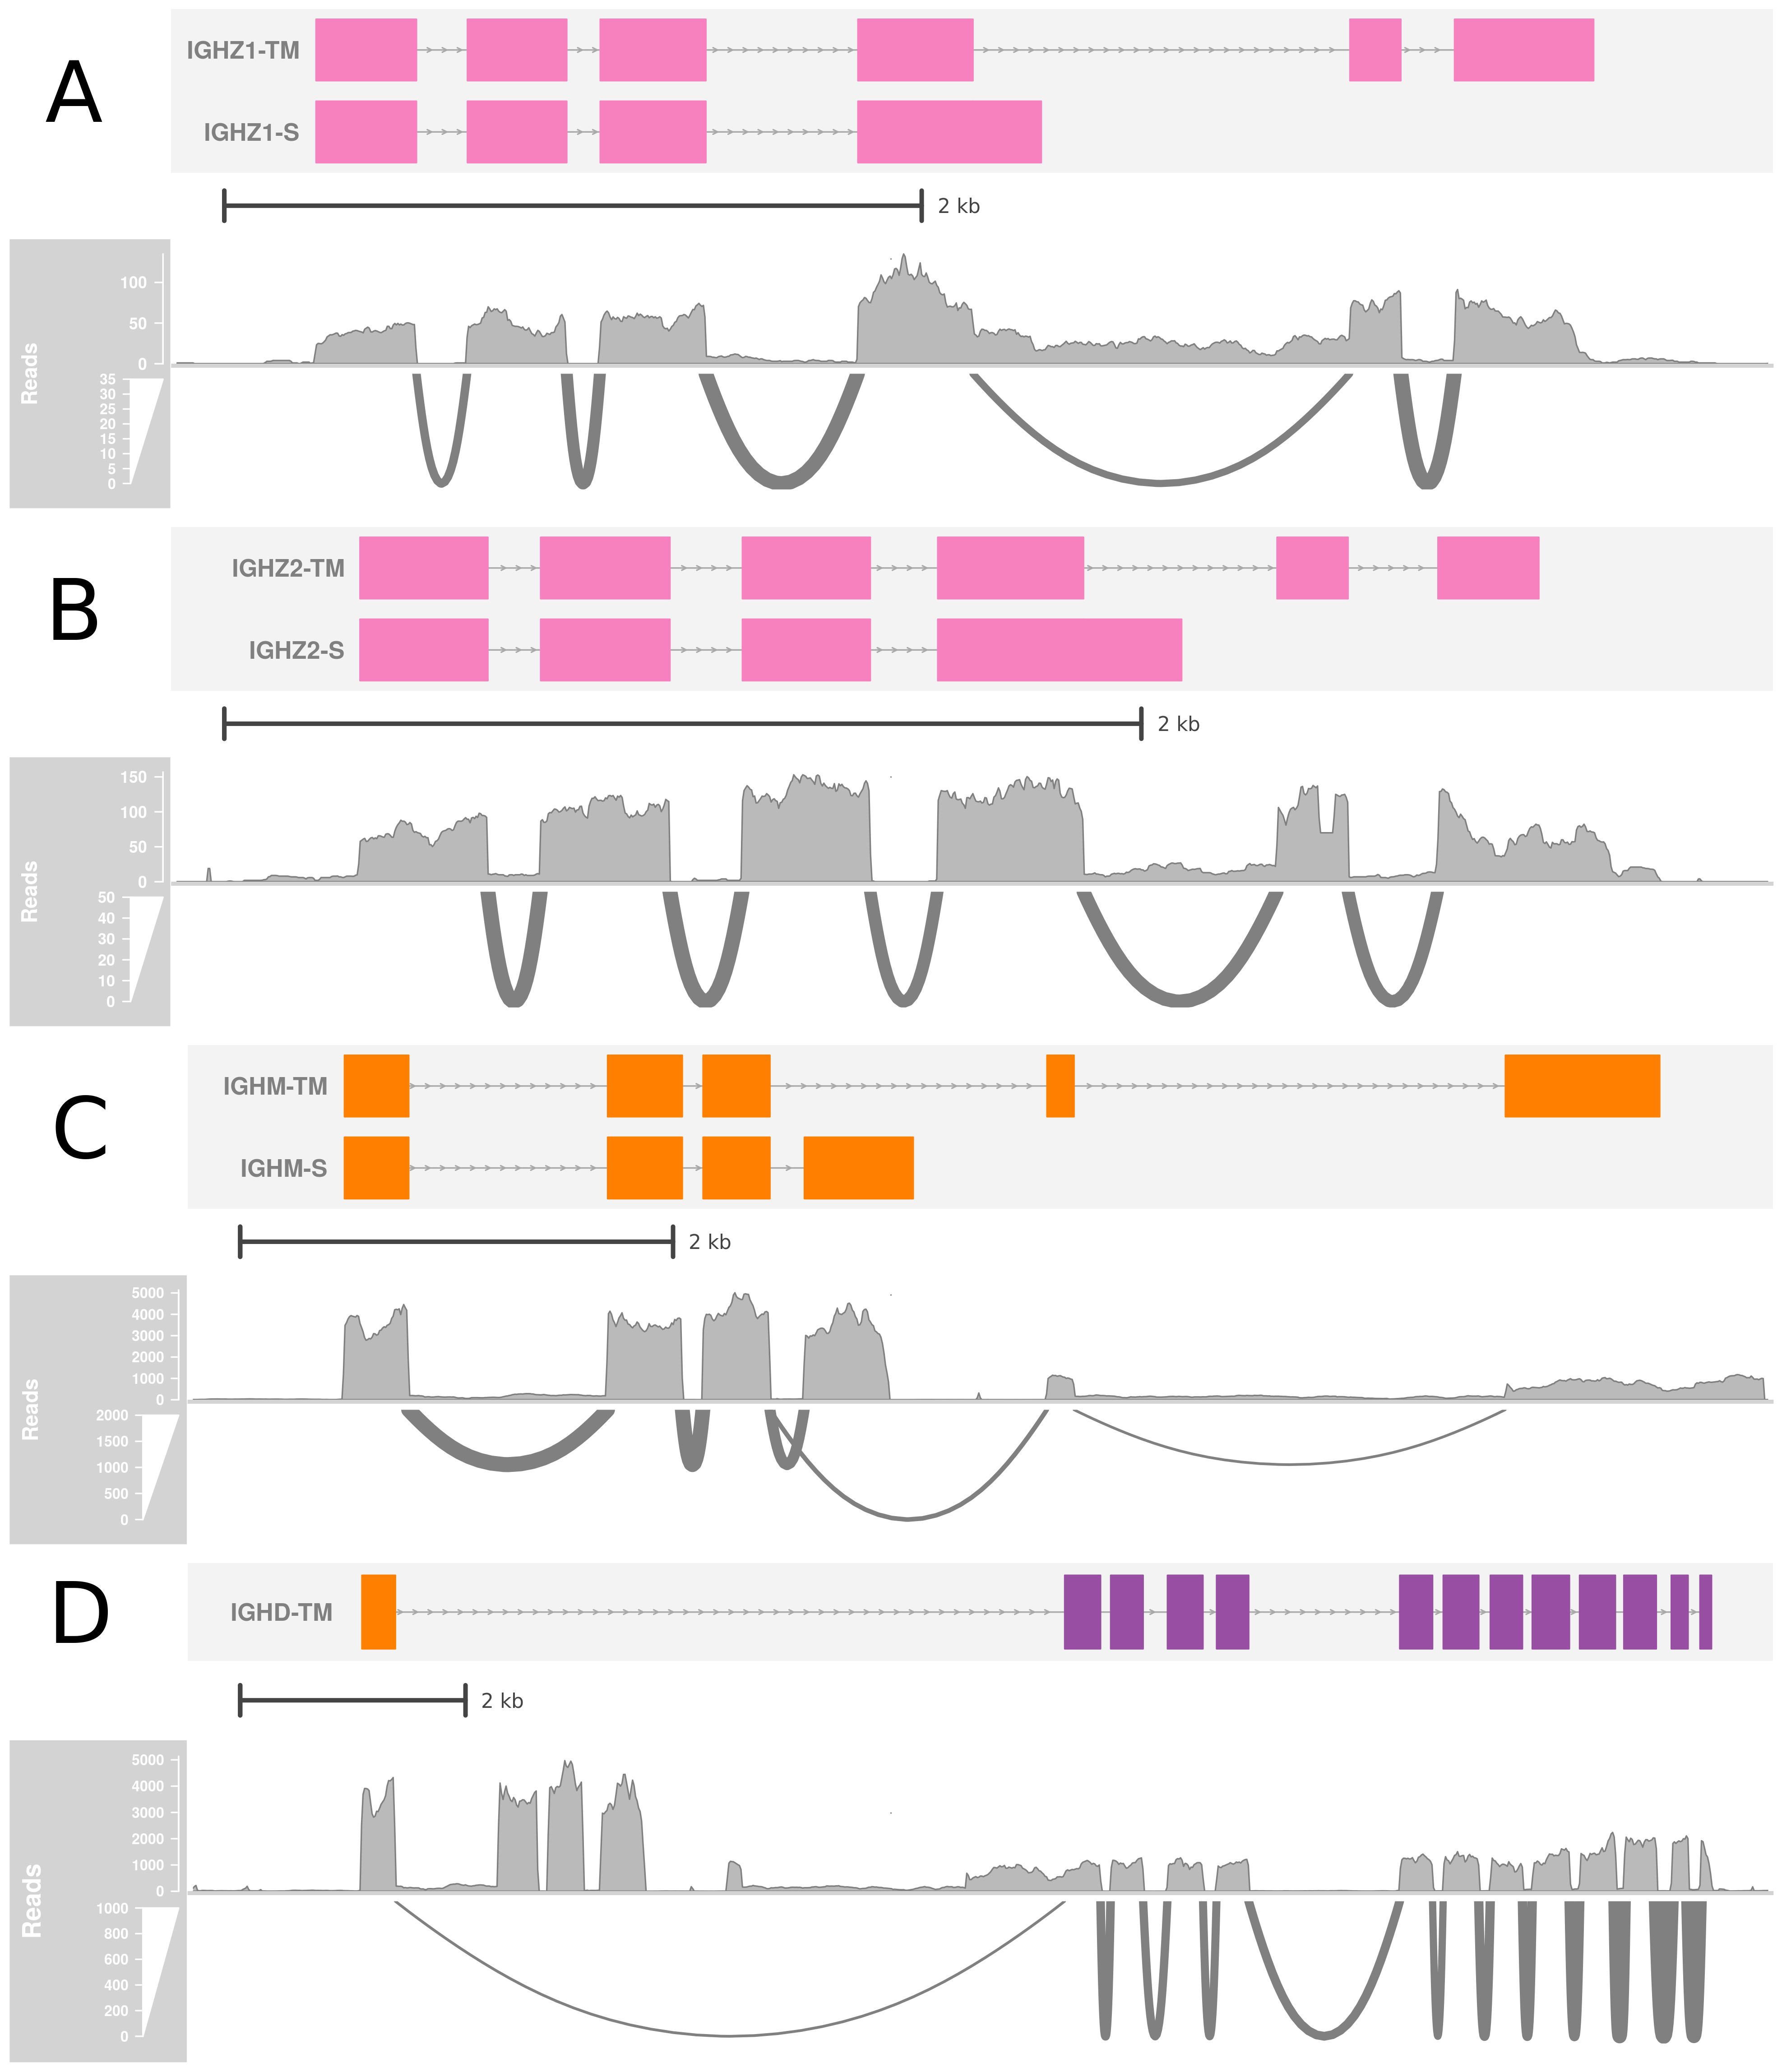
\includegraphics[width=\textwidth]{_Figures/png/xma-new-locus-sashimi}
	    \begin{subfigure}{0em}
        \phantomsubcaption{}
        \label{fig:xma-locus-sashimi-z1}
    \end{subfigure}
    \begin{subfigure}{0em}
        \phantomsubcaption{}
        \label{fig:xma-locus-sashimi-z2}
    \end{subfigure}
	\begin{subfigure}{0em}
        \phantomsubcaption{}
        \label{fig:xma-locus-sashimi-m}
    \end{subfigure}
    \begin{subfigure}{0em}
        \phantomsubcaption{}
        \label{fig:xma-locus-sashimi-d}
    \end{subfigure}
	\caption[Constant-region isoforms in \Xma]{\textbf{Constant-region isoforms in \Xma:} Coverage and sashimi plots of STAR-aligned RNA-seq reads from \Xma samples, demonstrating the splicing behaviour of \igh{} constant-region isoforms. (A) \igh{Z1} exon splicing, showing alternative use of the \cz{4}/TM1 splice junction and the post-\cz{4} secretory tail; (B) \igh{Z2} exon splicing; (C) IGHM exon splicing, showing alternative splicing patterns of IGHM-TM and IGHM-S; (D) IGHD exon splicing, including splicing of \cm{1} to \cd{1}.}
	\label{fig:xma-locus-sashimi}
	\end{figure}

	
\subsection{Variable regions}
\label{sec:xma-locus-variable}

In total, 125 \vh segments, 14 \dh segments and 15 \jh segments were identified in the \Xma IGH locus (\Cref{fig:xma-locus-map-b}). Of these, exactly one \vh (\igh{V01-01}), \dh (\igh{DZ01}) and \jh (\igh{JZ01}) lie upstream of the \igh{Z1} constant region, indicating that the variable-region sequence diversity available to this isotype is limited to a single VDJ combination. In contrast, the variable region between the end of \igh{Z1} and the start of \igh{Z2} is highly expanded, with 124 tightly-clustered \vh segments -- more than five times the total number seen in \Nfu, and more than seven times the number in the largest \Nfu sublocus. Of these 124 \vh segments, 106 (\pc{86}) are apparently functional, with the remainder pseudogenised by a variety of frameshift mutations, nonsense mutations, or truncation events (\Cref{tab:xma-vh-coords-1,tab:xma-vh-coords-2,tab:xma-vh-coords-3,tab:xma-vh-coords-4,tab:xma-vh-coords-5}); it remains to be seen whether \igh{V01-01} is also capable of recombining with \dh segments downstream of the \igh{Z1} constant region, and so constitutes part of the range of VDJ combinations available to the other constant regions. The \vh sequences in the \Xma locus are much more tightly packed than in the \Nfu locus, consistent with a lower overall prevalence of repetitive regions (21\%) in the \Xma genome \parencite{yuan2018repeats}.
	
In total, the \vh regions in \Xma \textit{IGH} fall into 23 families, of which eight contain multiple segments (\Cref{fig:xma-vh-families-tree,fig:xma-vh-families-map}); strikingly, the single \vh segment serving IGHZ (\igh{V01-01}) represents a separate family which is distinct from any other segment in the locus. To further investigate the evolutionary history of these families, the \vh segments from both the \Xma and \Nfu \igh{} loci were aligned together with \program{PRANK}, and the resulting alignment was used to construct a phylogenetic tree with \program{RAxML} \parencite{stamatakis2014raxml8,stamatakis2005raxml3,stamatakis2006raxml6}; the resulting tree (\Cref{fig:nfu-xma-vh-tree-nt}) revealed a clear interrelationship between the largest families in both loci (\Xma V02 and \Nfu V1), with a similar relationship observed for the second-largest families (\Xma V03 and \Nfu V2). 
In accordance with the close sequence relationship noted in \Cref{sec:nfu-locus-variable}, \Nfu V4 falls comfortably within the V03/V2 subtree, supporting its status as a pseudogenised subfamily of \Nfu V2.
		
In addition to its highly expanded \vh region, the variable region of the \Xma locus is unusual in the arrangement of its \dh and \jh segments (\Cref{tab:xma-dh-coords-seg,tab:xma-jh-coords-seg}): in addition to the relatively densely-packed blocks of four \dh and eight \jh regions between \igh{Z1} and \igh{M}, and the smaller groups of three \dh segments and one \jh segment between the last \vh segment and \igh{Z1}, small numbers of \dh and \jh segments are interspersed between blocks of \vh segments in the extended V-region between \igh{Z1} and \igh{Z2} (\Cref{fig:xma-locus-map-b}). Many of these segments are arranged such that groups of one or two \dh segments are closely associated with a single \jh segment, raising the possibility of a more cluster-like behaviour in which each VDJ group acts as a distinct recombination unit. However, the presence of larger D- and J-regions more closely upstream of the constant regions suggests a more conventional translocon behaviour; it remains to be seen which of these traditional models of antigen-receptor structure more closely matches the \textit{in vivo} recombination behaviour of this locus.
		
Finally, as is the case with \Nfu, the recombination signal sequences (RSSs) in \Xma IGH correspond closely to the standard expectations across the vertebrates, with the expected heptamer and nonamer consensus sequences and spacer length distributions (\Cref{fig:xma-rss-seqlogo-all,fig:xma-rss-seqlogo-sep}, 97.6\% of RSS spacers within \bp{1} of the expected conserved length).	
	
	\begin{figure}
	\centering
	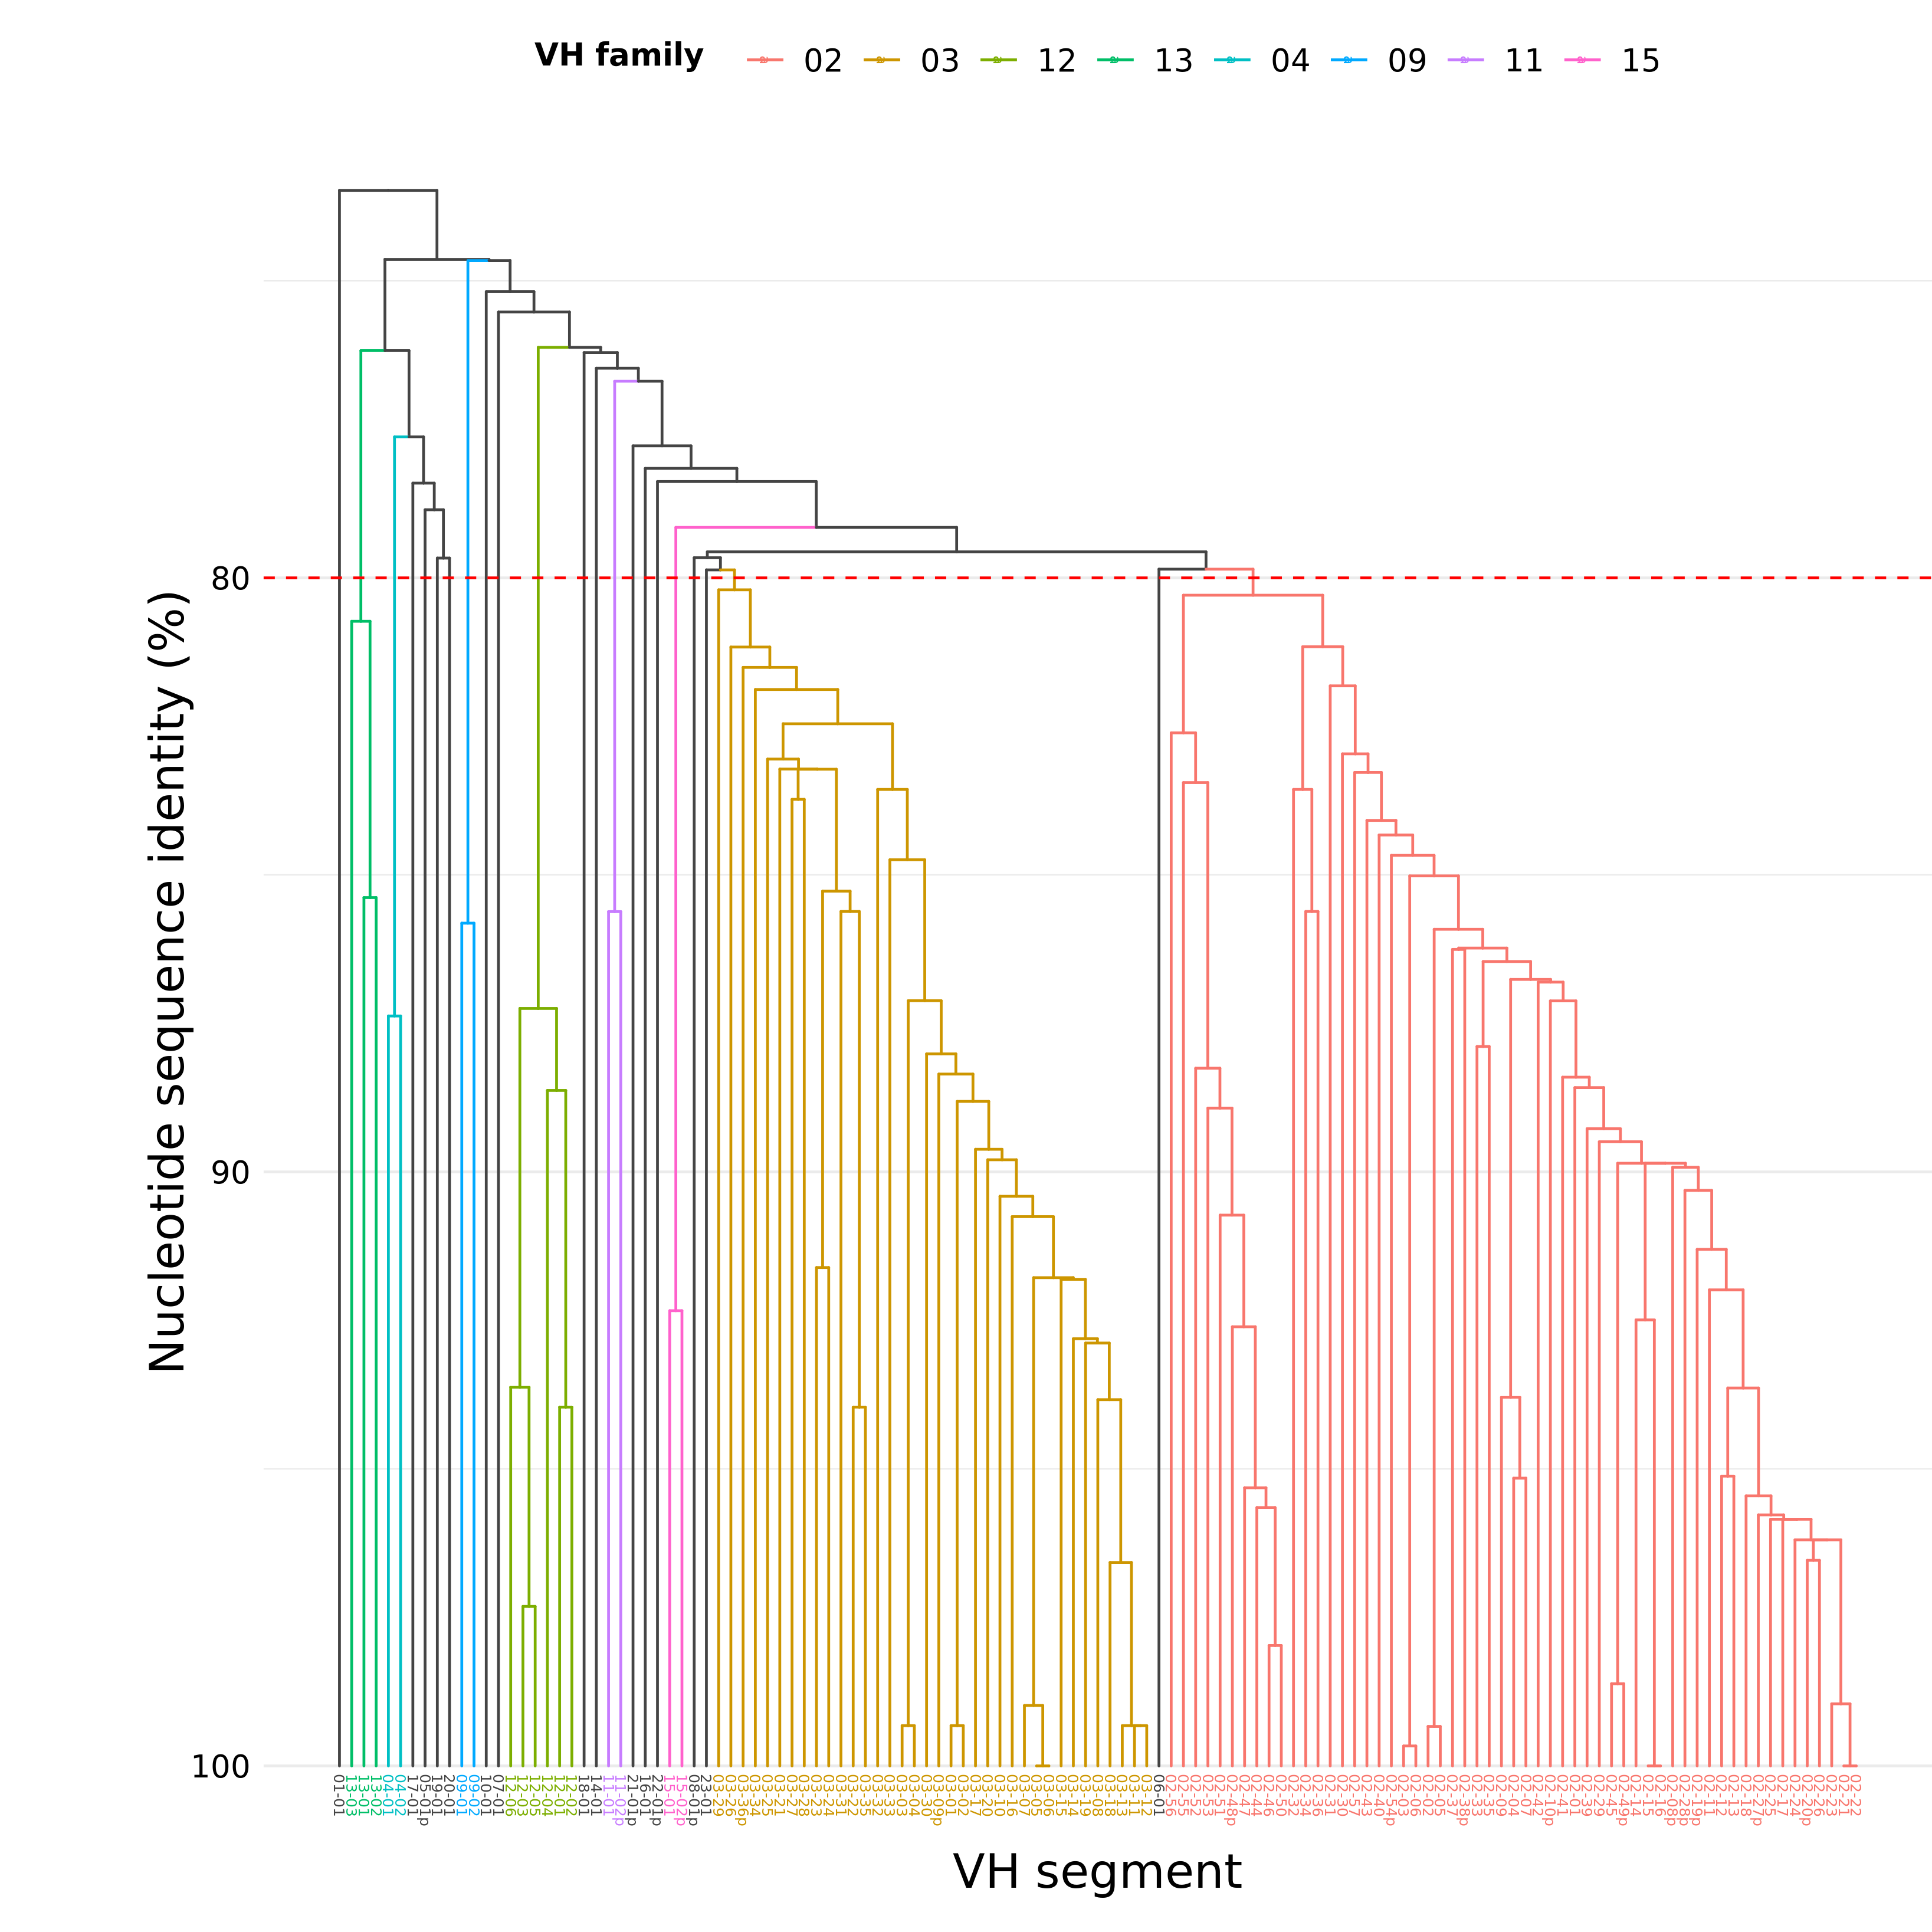
\includegraphics[width=\textwidth]{_Figures/png/xma-vh-families-tree}
	\caption[Dendrogram of \vh families in the in \Xma \textit{IgH} locus]{\textbf{Dendrogram of \vh families in the in \Xma (\textit{IgH}) locus:} Dendrogram of sequence similarity of \vh segments in the \Xma locus, arranged by single-linkage clustering on nucleotide sequence identity. The red line indicates the 80\% cutoff point for family assignment, while branch colour indicates family membership:  \vh families containing multiple segments are uniquely coloured, while single-segment families are in grey.}
	\label{fig:xma-vh-families-tree}
	\end{figure}
	
	\begin{figure}
	\centering
	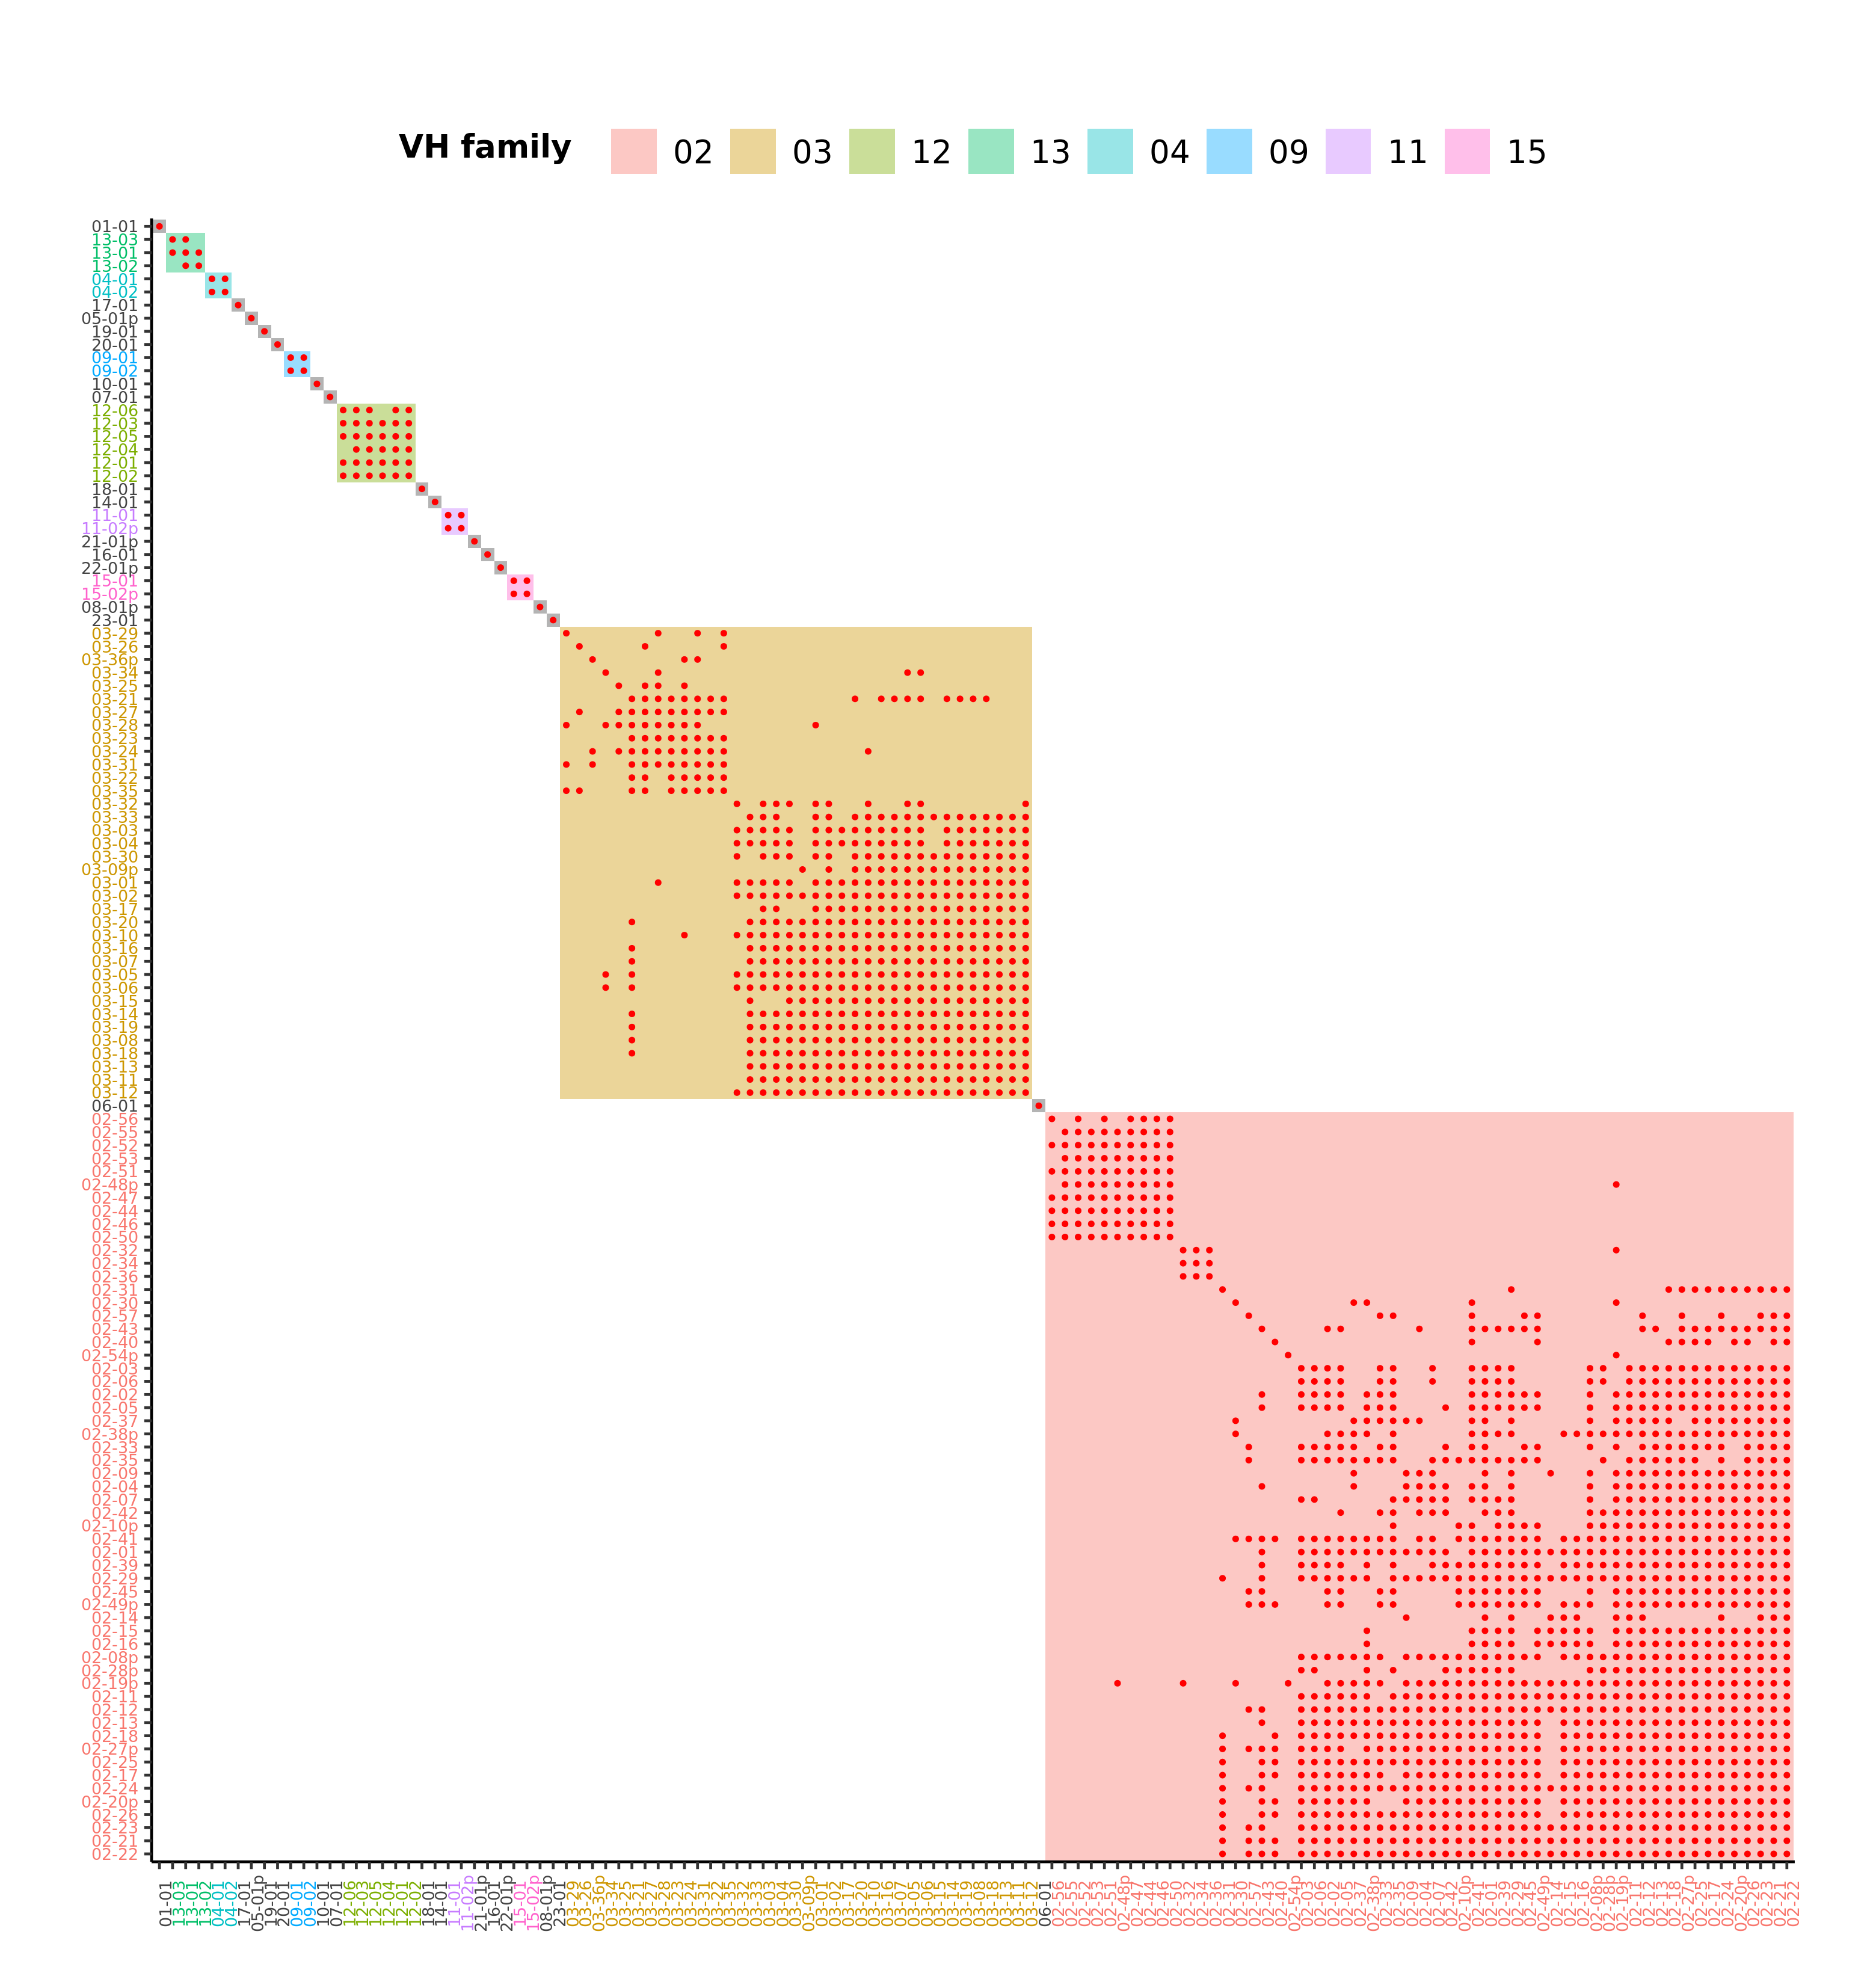
\includegraphics[width=\textwidth]{_Figures/png/xma-vh-families-map}
	\caption[Heatmap of \vh families in the in \Xma \textit{IgH} locus]{\textbf{Heatmap of \vh families in the in \Xma (\textit{IgH}) locus:} Heatmap of family relationships among \Xma \vh segments, with coloured shading indicating families and red dots indicating pairwise nucleotide sequence identity of at least 80\%. \vh families containing multiple segments are uniquely coloured, while single-segment families are in grey.}
	\label{fig:xma-vh-families-map}
	\end{figure}
	
	\begin{figure}
	\centering
	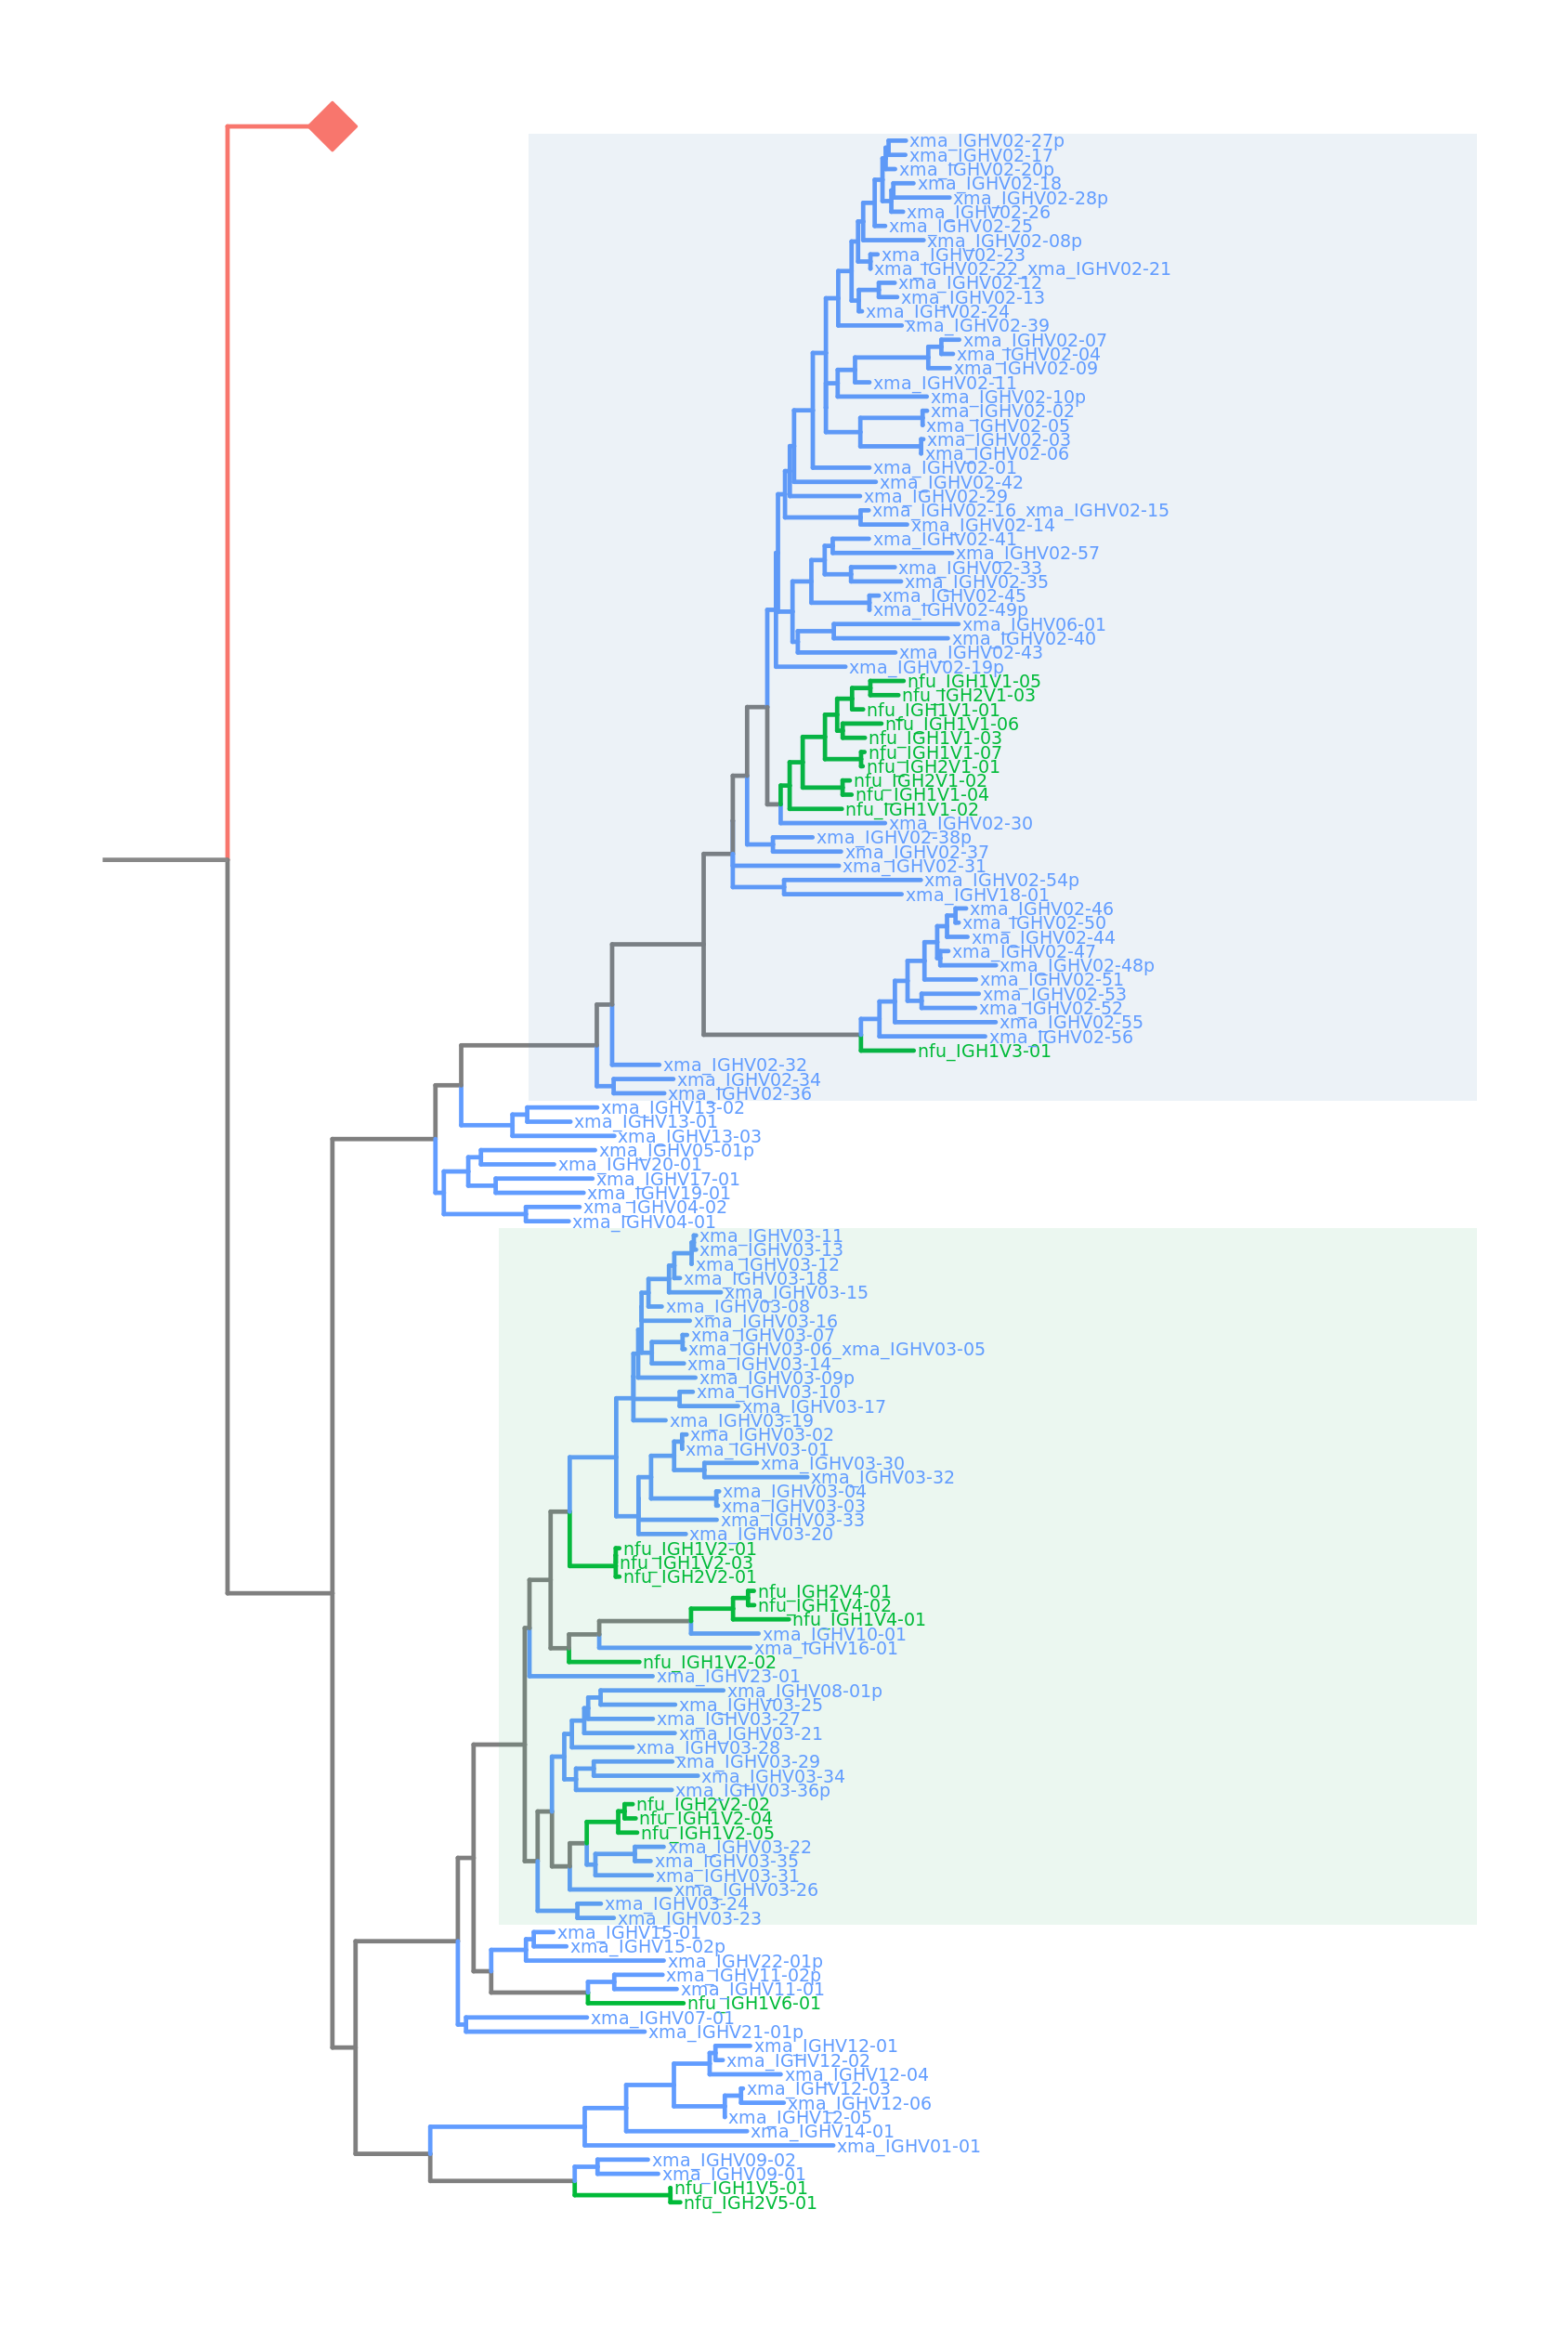
\includegraphics[width=0.8\textwidth]{_Figures/png/nfu-xma-vh-tree-nt.png}
	\caption[Evolutionary relationships between \vh families in \Xma and \Nfu]{\textbf{Evolutionary relationships between \vh families in \Xma and \Nfu:} Phylogenetic tree of evolutionary relationships between \textit{IGH} \vh segments in \Nfu and \Xma, as inferred from the nucleotide sequences of \vh segments from both loci. Note the close interrelationship between the largest (blue zone) and second-largest (green zone) families in each species. The red diamond indicates the location of the outgroup, which is composed of zebrafish \textit{TRB} V-segments.}
	\label{fig:nfu-xma-vh-tree-nt}
	\end{figure}
	
	\begin{figure}
		\begin{subfigure}{0em}
        \phantomsubcaption{}
        \label{fig:xma-rss-seqlogo-all-heptamer}
    \end{subfigure}
    \begin{subfigure}{0em}
        \phantomsubcaption{}
        \label{fig:xma-rss-seqlogo-all-spacer}
    \end{subfigure}
    \begin{subfigure}{0em}
        \phantomsubcaption{}
        \label{fig:xma-rss-seqlogo-all-nonamer}
    \end{subfigure}
	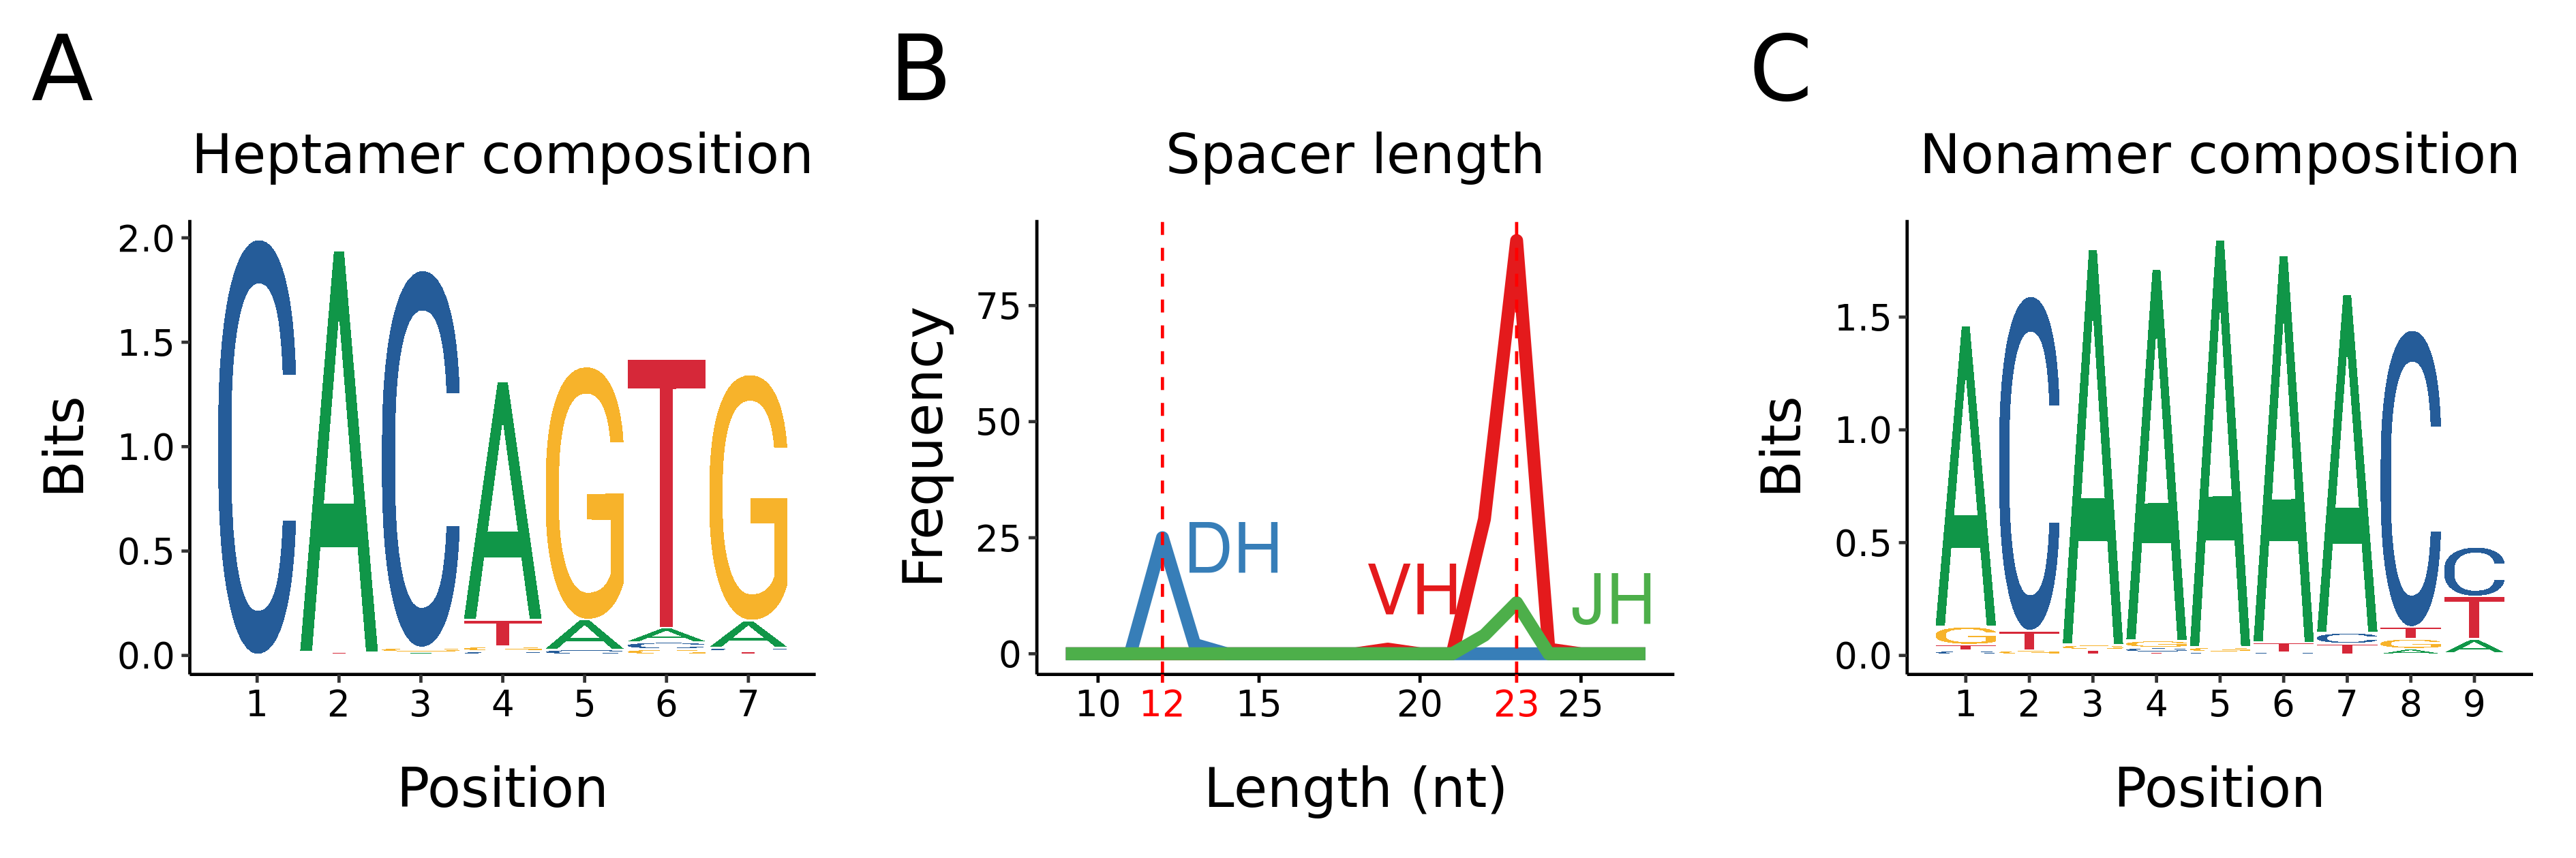
\includegraphics[width=\textwidth]{_Figures/png/xma-new-rss-seqlogo-all}
	\caption[Recombination signal sequences in the \Xma \textit{IGH} locus]{\textbf{Recombination signal sequences in the \Xma \textit{IGH} locus:} (A) Sequence composition of conserved heptamer sequences across all \Xma heavy-chain RSSs; (B) length distribution of unconserved spacer sequences in \Xma heavy-chain RSSs; (C) sequence composition of conserved heptamer sequences across all \Xma heavy-chain RSSs.}
	\label{fig:xma-rss-seqlogo-all}
	\end{figure}
	
	\begin{figure}
	\centering
	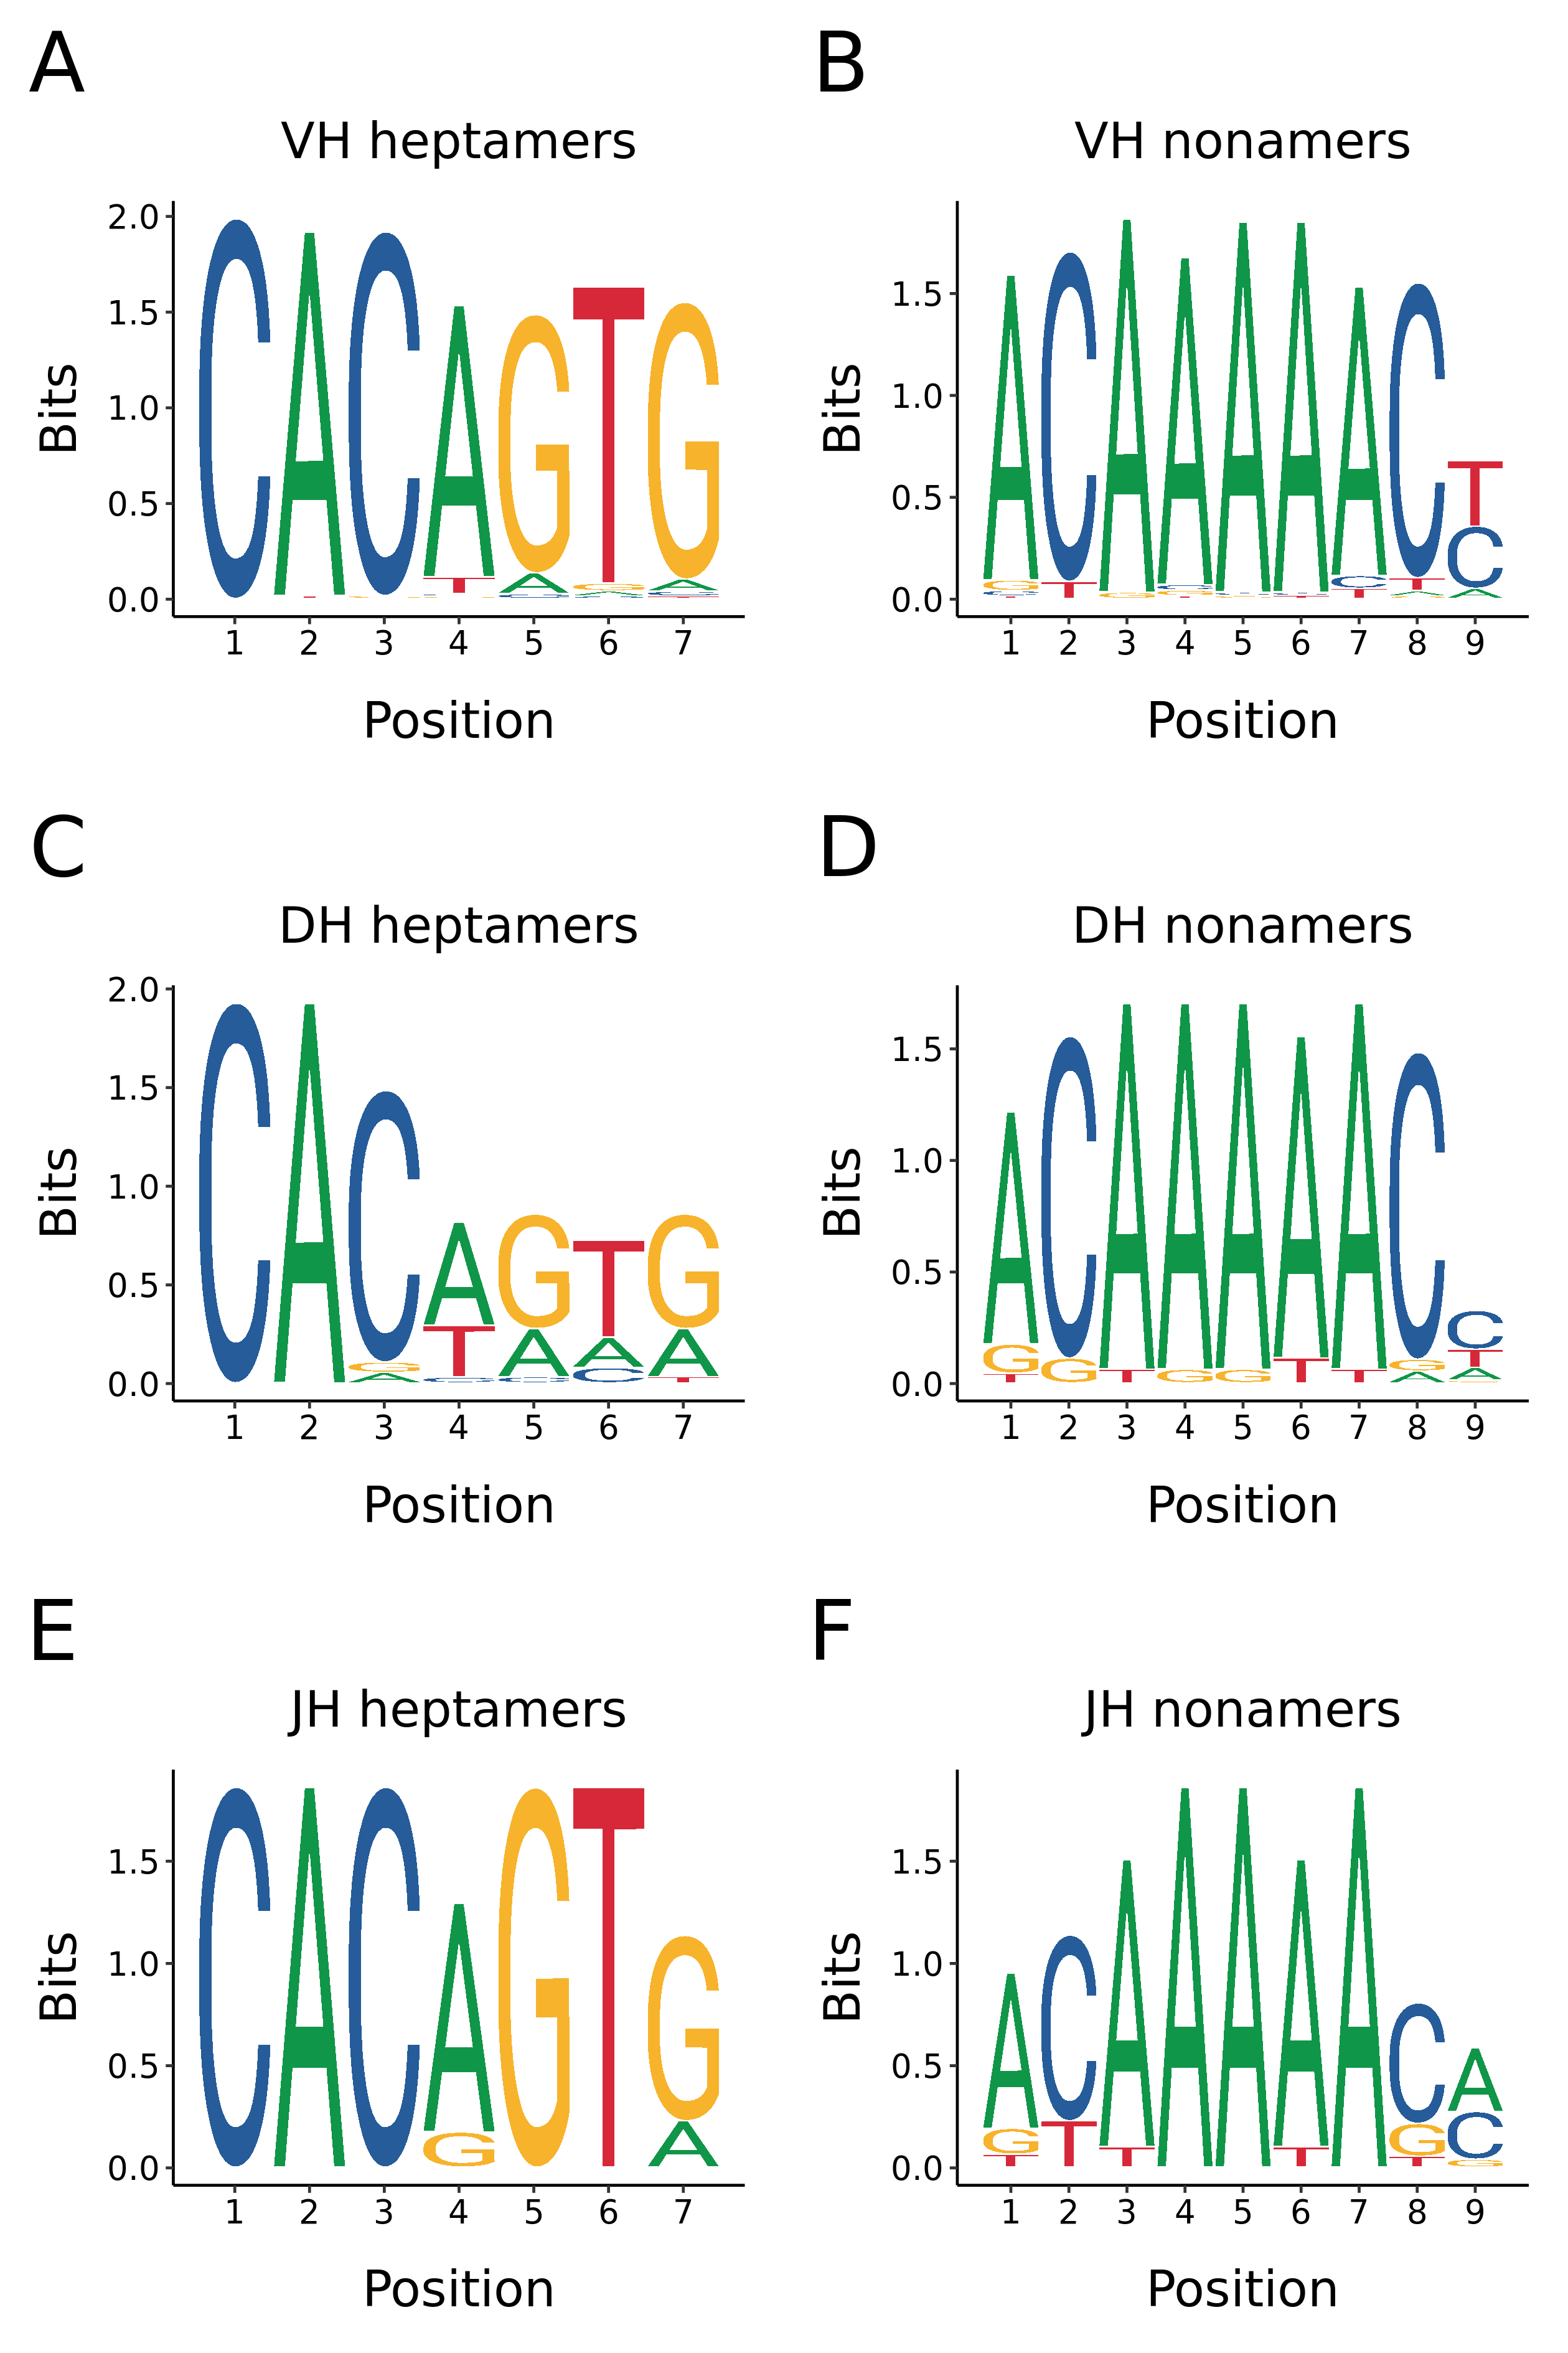
\includegraphics[width=0.9\textwidth]{_Figures/png/xma-new-rss-seqlogo-sep}
	\caption[\Xma recombination signal sequences by segment type]{\textbf{\Xma recombination signal sequences by segment type:} Sequence composition of conserved heptamer (A,C,E) and nonamer (B,D,F) sequences from \Xma heavy-chain RSSs associated with \vh (A,B), \dh (C,D) or \jh (E,F) gene segments.}
	\label{fig:xma-rss-seqlogo-sep}
	\end{figure}

\FloatBarrier

	
\afterpage{%
    \begin{landscape}
        \centering
        \vspace*{\fill}
        \scriptsize
		% latex table generated in R 3.5.2 by xtable 1.8-3 package
% Tue Jan  8 15:33:33 2019
\begin{tabular}{lrrrlrlllrrl}
  \toprule Name & Start & End & Length & Strand & RSS Start & Heptamer & Spacer Length & Nonamer & RSS End & RSS Length & Comment \\ 
  \midrule IGHV01-01 & 1159 & 1450 & 292 & + & 1451 & CACAGTG & 23 & GTAAAAACC & 1489 & 39 &  \\ 
  IGHV02-01 & 10534 & 10825 & 292 & + & 10826 & CACAGTG & 23 & ACAAAACCC & 10864 & 39 &  \\ 
  IGHV02-02 & 11961 & 12261 & 301 & + & 12262 & CACTGTG & 23 & ACAAAAACT & 12300 & 39 &  \\ 
  IGHV02-03 & 13319 & 13616 & 298 & + & 13617 & CACAGTG & 23 & ACACAAACT & 13655 & 39 &  \\ 
  IGHV03-01 & 15440 & 15734 & 295 & + & 15735 & CACAGTG & 22 & ACAAAAACT & 15772 & 38 &  \\ 
  IGHV02-04 & 16618 & 16908 & 291 & + & 16909 & CACAGTG & 23 & ACAAAAACC & 16947 & 39 &  \\ 
  IGHV02-05 & 17522 & 17822 & 301 & + & 17823 & CACTGTG & 22 & ACAAAAACT & 17860 & 38 &  \\ 
  IGHV02-06 & 18881 & 19178 & 298 & + & 19179 & CACAGTG & 23 & ACACAAACT & 19217 & 39 &  \\ 
  IGHV03-02 & 21000 & 21294 & 295 & + & 21295 & CACAGTG & 22 & ACAAAAACT & 21332 & 38 &  \\ 
  IGHV02-07 & 22179 & 22467 & 289 & + & 22468 & CACAGTG & 23 & ACAAAAACC & 22506 & 39 &  \\ 
  IGHV02-08p & 24234 & 24514 & 281 & + & 24515 & CACAGTG & 23 & ACAAAAACT & 24553 & 39 & Frameshift \\ 
  IGHV04-01 & 25359 & 25659 & 301 & + & 25660 & CACAGTG & 23 & ACAAAAACT & 25698 & 39 &  \\ 
  IGHV04-02 & 27066 & 27366 & 301 & + & 27367 & CACAGTG & 23 & ACAAAAACA & 27405 & 39 &  \\ 
  IGHV02-09 & 28669 & 28958 & 290 & + & 28959 & CACAGTG & 23 & ACAAAAACC & 28997 & 39 &  \\ 
  IGHV02-10p & 30460 & 30741 & 282 & + & 30742 & CACAATG & 23 & ACAAAACTC & 30780 & 39 & Frameshift \\ 
  IGHV02-11 & 32395 & 32681 & 287 & + & 32682 & CACAGTG & 23 & ACAAAAACC & 32720 & 39 &  \\ 
  IGHV03-03 & 33663 & 33957 & 295 & + & 33958 & CACTGTG & 22 & ACAAAAACT & 33995 & 38 &  \\ 
  IGHV02-12 & 35012 & 35299 & 288 & + & 35300 & CACAGTG & 23 & ACAAAAACC & 35338 & 39 &  \\ 
  IGHV03-04 & 36281 & 36575 & 295 & + & 36576 & CACTGTG & 22 & ACAAAAACT & 36613 & 38 &  \\ 
  IGHV02-13 & 37639 & 37931 & 293 & + & 37932 & CACAGTG & 23 & ACAAAAACT & 37970 & 39 &  \\ 
  IGHV02-14 & 39019 & 39311 & 293 & + & 39312 & CACAGTG & 23 & ACAAAAACT & 39350 & 39 &  \\ 
  IGHV03-05 & 41008 & 41302 & 295 & + & 41303 & CACAGTG & 22 & ACAAAAACT & 41340 & 38 &  \\ 
  IGHV02-15 & 42660 & 42952 & 293 & + & 42953 & CACAGTG & 23 & ACAAAAACT & 42991 & 39 &  \\ 
  IGHV03-06 & 45081 & 45375 & 295 & + & 45376 & CACAGTG & 22 & ACAAAAACT & 45413 & 38 &  \\ 
  IGHV02-16 & 46732 & 47024 & 293 & + & 47025 & CACAGTG & 23 & ACAAAAACT & 47063 & 39 &  \\ 
   \bottomrule \end{tabular}

		\normalsize\vspace{1em}
        \captionof{table}{Co-ordinate table of \vh segments in the \xma \igh{} locus, part 1.}
        \label{tab:xma-vh-coords-1}
        \vspace*{\fill}
    \end{landscape}
}

\afterpage{%
    \begin{landscape}
        \centering
        \vspace*{\fill}
        \scriptsize
		% latex table generated in R 3.5.2 by xtable 1.8-3 package
% Tue Jan  8 15:33:33 2019
\begin{tabular}{lrrrlrlllrrl}
  \toprule Name & Start & End & Length & Strand & RSS Start & Heptamer & Spacer Length & Nonamer & RSS End & RSS Length & Comment \\ 
  \midrule IGHV03-07 & 48618 & 48912 & 295 & + & 48913 & CACAGTG & 22 & ACAAAAACT & 48950 & 38 &  \\ 
  IGHV02-17 & 50323 & 50611 & 289 & + & 50612 & CACAGTG & 23 & ACAAAAACC & 50650 & 39 &  \\ 
  IGHV03-08 & 51890 & 52184 & 295 & + & 52185 & CACAGTG & 22 & ACAAAAACT & 52222 & 38 &  \\ 
  IGHV03-09p & 53026 & 53274 & 249 & + & 53275 &  &  &  &  &  & 3'-truncated, no RSS \\ 
  IGHV02-18 & 54462 & 54747 & 286 & + & 54748 & CACAGTG & 23 & ACAAAAACC & 54786 & 39 &  \\ 
  IGHV02-19p & 55729 & 55866 & 138 & + & 55867 & CACAGTG & 23 & ACAAAAACC & 55905 & 39 & 3'-truncated \\ 
  IGHV03-10 & 57371 & 57662 & 292 & + & 57663 & CACAGTG & 22 & ACAAAAACT & 57700 & 38 &  \\ 
  IGHV02-20p & 58698 & 58986 & 289 & + & 58987 & CACAGTG & 23 & ATAAAAACC & 59025 & 39 & Nonsense mutation \\ 
  IGHV03-11 & 59940 & 60234 & 295 & + & 60235 & CACAGTG & 22 & ACAAAAACT & 60272 & 38 &  \\ 
  IGHV02-21 & 61249 & 61537 & 289 & + & 61538 & CACAGTG & 23 & ATAAAAACC & 61576 & 39 &  \\ 
  IGHV03-12 & 62491 & 62785 & 295 & + & 62786 & CACAGTG & 22 & ACAAAAACT & 62823 & 38 &  \\ 
  IGHV02-22 & 63801 & 64089 & 289 & + & 64090 & CACAGTG & 23 & ATAAAAACC & 64128 & 39 &  \\ 
  IGHV03-13 & 65043 & 65337 & 295 & + & 65338 & CACAGTG & 22 & ACAAAAACT & 65375 & 38 &  \\ 
  IGHV02-23 & 66354 & 66640 & 287 & + & 66641 & CACAGTG & 23 & ACAAAAACT & 66679 & 39 &  \\ 
  IGHV03-14 & 68452 & 68743 & 292 & + & 68744 & CACTATG & 22 & ACAAAACTC & 68781 & 38 &  \\ 
  IGHV02-24 & 70101 & 70389 & 289 & + & 70390 & CACAGTG & 23 & ACAAAAACC & 70428 & 39 &  \\ 
  IGHV03-15 & 72206 & 72501 & 296 & + & 72502 & CACAGTG & 22 & ACAAAAACT & 72539 & 38 &  \\ 
  IGHV02-25 & 73484 & 73772 & 289 & + & 73773 & CACAGTG & 23 & ACAAAAACC & 73811 & 39 &  \\ 
  IGHV03-16 & 75799 & 76090 & 292 & + & 76091 & CACAGTG & 22 & ACAAAAACT & 76128 & 38 &  \\ 
  IGHV03-17 & 77773 & 78067 & 295 & + & 78068 & CACAGTG & 22 & ACAAAAACT & 78105 & 38 &  \\ 
  IGHV02-26 & 79001 & 79289 & 289 & + & 79290 & CACAGTG & 23 & ACAAAAACC & 79328 & 39 &  \\ 
  IGHV03-18 & 80492 & 80784 & 293 & + & 80785 & CACAGTG & 22 & ACAAAAACT & 80822 & 38 &  \\ 
  IGHV02-27p & 81799 & 82082 & 284 & + & 82083 & CACAGTG & 23 & ACAAAAACC & 82121 & 39 & Frameshift \\ 
  IGHV03-19 & 83736 & 84030 & 295 & + & 84031 & CACAGTG & 22 & ACAAAAACT & 84068 & 38 &  \\ 
  IGHV02-28p & 85093 & 85381 & 289 & + & 85382 & CACAGGG & 23 & GCAAAAACC & 85420 & 39 & Nonsense mutation \\ 
   \bottomrule \end{tabular}

		\normalsize\vspace{1em}
        \captionof{table}{Co-ordinate table of \vh segments in the \xma \igh{} locus, part 2.}
        \label{tab:xma-vh-coords-2}
        \vspace*{\fill}
    \end{landscape}
}

\afterpage{%
    \begin{landscape}
        \centering
        \vspace*{\fill}
        \scriptsize
		% latex table generated in R 3.5.2 by xtable 1.8-3 package
% Tue Jan  8 15:33:33 2019
\begin{tabular}{lrrrlrlllrrl}
  \toprule Name & Start & End & Length & Strand & RSS Start & Heptamer & Spacer Length & Nonamer & RSS End & RSS Length & Comment \\ 
  \midrule IGHV02-29 & 86225 & 86505 & 281 & + & 86506 & CACAGTG & 23 & ATAAAAACC & 86544 & 39 &  \\ 
  IGHV03-20 & 87419 & 87713 & 295 & + & 87714 & CACAGTG & 22 & ACAAAAACT & 87751 & 38 &  \\ 
  IGHV03-21 & 94532 & 94826 & 295 & + & 94827 & CACAGTG & 23 & ACAAAAACC & 94865 & 39 &  \\ 
  IGHV03-22 & 96192 & 96489 & 298 & + & 96490 & CACAGTG & 23 & ACAAAAACC & 96528 & 39 &  \\ 
  IGHV03-23 & 98068 & 98368 & 301 & + & 98369 & CACAGTG & 23 & ACAAAAACC & 98407 & 39 &  \\ 
  IGHV03-24 & 99482 & 99779 & 298 & + & 99780 & CACAGTG & 23 & ACAAAAACC & 99818 & 39 &  \\ 
  IGHV03-25 & 101639 & 101936 & 298 & + & 101937 & CACAGTG & 23 & ACAAAAACC & 101975 & 39 &  \\ 
  IGHV05-01p & 102818 & 103096 & 279 & + & 103097 & CAGAAGC & 0 & ACAAAAACT & 103112 & 16 & Frameshift \\ 
  IGHV03-26 & 104098 & 104389 & 292 & + & 104390 & CACAGTG & 23 & ACAAAATCC & 104428 & 39 &  \\ 
  IGHV06-01 & 105551 & 105831 & 281 & + & 105832 & CACAGTG & 23 & ACAAAAACC & 105870 & 39 &  \\ 
  IGHV03-27 & 107274 & 107571 & 298 & + & 107572 & CACAGTG & 23 & ACAAAAACC & 107610 & 39 &  \\ 
  IGHV03-28 & 108775 & 109072 & 298 & + & 109073 & CACAGAG & 23 & ACAAAAACC & 109111 & 39 &  \\ 
  IGHV03-29 & 110372 & 110672 & 301 & + & 110673 & CACAGTG & 23 & ACAAAAACC & 110711 & 39 &  \\ 
  IGHV07-01 & 111565 & 111856 & 292 & + & 111857 & CACAATG & 23 & ACAAAAACT & 111895 & 39 &  \\ 
  IGHV08-01p & 113033 & 113330 & 298 & + & 113331 & CACAGAG & 23 & CCAAGAACC & 113369 & 39 & Nonsense mutation \\ 
  IGHV09-01 & 115512 & 115800 & 289 & + & 115801 & CACAGTG & 22 & ACAAAAACT & 115838 & 38 &  \\ 
  IGHV10-01 & 117078 & 117379 & 302 & + & 117380 & CACAGTG & 22 & ACATAAACT & 117417 & 38 &  \\ 
  IGHV11-01 & 119462 & 119760 & 299 & + & 119761 & CACAGTG & 23 & ACAAAAACT & 119799 & 39 &  \\ 
  IGHV03-30 & 126125 & 126416 & 292 & + & 126417 & CACAGTG & 22 & ACAAAAACC & 126454 & 38 &  \\ 
  IGHV03-31 & 127109 & 127400 & 292 & + & 127401 & CACAGTG & 23 & GCAAAAACC & 127439 & 39 &  \\ 
  IGHV12-01 & 128489 & 128786 & 298 & + & 128787 & CACAGTG & 23 & ACAAAAACC & 128825 & 39 &  \\ 
  IGHV02-30 & 135711 & 136000 & 290 & + & 136001 & CACAGTG & 22 & ACAAAAACA & 136038 & 38 &  \\ 
  IGHV13-01 & 136757 & 137057 & 301 & + & 137058 & CACAGTG & 23 & ACAAAAACT & 137096 & 39 &  \\ 
  IGHV02-31 & 138344 & 138637 & 294 & + & 138638 & CACAGTG & 23 & ACAAAAATC & 138676 & 39 &  \\ 
  IGHV02-32 & 140024 & 140315 & 292 & + & 140316 & CACTGTG & 23 & ACAAAAACT & 140354 & 39 &  \\ 
   \bottomrule \end{tabular}

		\normalsize\vspace{1em}
        \captionof{table}{Co-ordinate table of \vh segments in the \xma \igh{} locus, part 3.}
        \label{tab:xma-vh-coords-3}
        \vspace*{\fill}
    \end{landscape}
}

\afterpage{%
    \begin{landscape}
        \centering
        \vspace*{\fill}
        \scriptsize
		% latex table generated in R 3.5.2 by xtable 1.8-3 package
% Tue Jan  8 15:33:33 2019
\begin{tabular}{lrrrlrlllrrl}
  \toprule Name & Start & End & Length & Strand & RSS Start & Heptamer & Spacer Length & Nonamer & RSS End & RSS Length & Comment \\ 
  \midrule IGHV02-33 & 142332 & 142620 & 289 & + & 142621 & CACAGTG & 23 & ACAAAAACA & 142659 & 39 &  \\ 
  IGHV02-34 & 144334 & 144625 & 292 & + & 144626 & CACAGTG & 23 & ACAAAAACT & 144664 & 39 &  \\ 
  IGHV02-35 & 145740 & 146031 & 292 & + & 146032 & CACAGTG & 23 & ACAAAAAAT & 146070 & 39 &  \\ 
  IGHV02-36 & 146903 & 147194 & 292 & + & 147195 & CACAGTG & 23 & ACAAAAACT & 147233 & 39 &  \\ 
  IGHV02-37 & 147839 & 148138 & 300 & + & 148139 & CACAGTG & 23 & ACAAAAATC & 148177 & 39 &  \\ 
  IGHV02-38p & 150504 & 150797 & 294 & + & 150798 & CACAATA & 23 & ACAAAAACC & 150836 & 39 & Nonsense mutation \\ 
  IGHV02-39 & 152249 & 152537 & 289 & + & 152538 & CACAGTA & 23 & ACAAAAACC & 152576 & 39 &  \\ 
  IGHV14-01 & 154075 & 154374 & 300 & + & 154375 & CACAGTG & 23 & ACAAAAAGT & 154413 & 39 &  \\ 
  IGHV02-40 & 155433 & 155709 & 277 & + & 155710 & CACAGTG & 23 & ACAAAAACC & 155748 & 39 &  \\ 
  IGHV02-41 & 156583 & 156870 & 288 & + & 156871 & CACAGTG & 23 & ACAAAAACC & 156909 & 39 &  \\ 
  IGHV02-42 & 163977 & 164269 & 293 & + & 164270 & CACAGTG & 23 & ACAAAACCC & 164308 & 39 &  \\ 
  IGHV03-32 & 165416 & 165708 & 293 & + & 165709 & CACAGTG & 22 & ACAAAAACA & 165746 & 38 &  \\ 
  IGHV02-43 & 166994 & 167293 & 300 & + & 167294 & CACAATG & 23 & ACAGAAACT & 167332 & 39 &  \\ 
  IGHV12-02 & 169602 & 169900 & 299 & + & 169901 & CACAGTG & 23 & ACAAAAACC & 169939 & 39 &  \\ 
  IGHV02-44 & 171452 & 171752 & 301 & + & 171753 & CACTGTG & 23 & GCAAAAACT & 171791 & 39 &  \\ 
  IGHV02-45 & 173096 & 173384 & 289 & + & 173385 & CTCAGTG & 23 & ACAAAAACC & 173423 & 39 &  \\ 
  IGHV02-46 & 174714 & 175009 & 296 & + & 175010 & CACAGTG & 23 & ACAAAAACT & 175048 & 39 &  \\ 
  IGHV02-47 & 176396 & 176697 & 302 & + & 176698 & CACAGTG & 23 & ACAAAAACT & 176736 & 39 &  \\ 
  IGHV12-03 & 178422 & 178719 & 298 & + & 178720 & CACAGTG & 23 & ACAAAAACA & 178758 & 39 &  \\ 
  IGHV12-04 & 181245 & 181543 & 299 & + & 181544 & CACAGTG & 23 & ACAAAAACC & 181582 & 39 &  \\ 
  IGHV02-48p & 182977 & 183236 & 260 & + & 183237 & CACAGGT & 8 & ACAAAAACT & 183260 & 24 & 5'-truncated \\ 
  IGHV02-49p & 184323 & 184611 & 289 & + & 184612 & CACAGTG & 23 & ACAAAAACC & 184650 & 39 & Nonsense mutation \\ 
  IGHV02-50 & 185946 & 186244 & 299 & + & 186245 & CACAGTG & 23 & ACAAAAACT & 186283 & 39 &  \\ 
  IGHV02-51 & 187624 & 187925 & 302 & + & 187926 & CACAGTG & 23 & ACAAAAACT & 187964 & 39 &  \\ 
  IGHV12-05 & 190987 & 191284 & 298 & + & 191285 & CACAGTG & 23 & ACAAAAACA & 191323 & 39 &  \\ 
   \bottomrule \end{tabular}

		\normalsize\vspace{1em}
        \captionof{table}{Co-ordinate table of \vh segments in the \xma \igh{} locus, part 4.}
        \label{tab:xma-vh-coords-4}
        \vspace*{\fill}
    \end{landscape}
}

\afterpage{%
    \begin{landscape}
        \centering
        \vspace*{\fill}
        \scriptsize
		% latex table generated in R 3.5.2 by xtable 1.8-3 package
% Tue Jan  8 15:33:35 2019
\begin{tabular}{lrrrlrlllrrp{4cm}}
  \toprule Name & Start & End & Length & Strand & RSS Start & Heptamer & Spacer Length & Nonamer & RSS End & RSS Length & Comment \\ 
  \midrule IGHV02-52 & 192570 & 192868 & 299 & + & 192869 & CACAGTG & 19 & CTGAAAACC & 192903 & 35 &  \\ 
  IGHV12-06 & 193608 & 193906 & 299 & + & 193907 & CACAGTG & 23 & ACAAAAACA & 193945 & 39 &  \\ 
  IGHV02-53 & 195271 & 195572 & 302 & + & 195573 & CACAGTG & 23 & ACAAAAACC & 195611 & 39 &  \\ 
  IGHV15-01 & 204396 & 204693 & 298 & + & 204694 & CACAATC & 23 & ACAAAAACT & 204732 & 39 &  \\ 
  IGHV13-02 & 206203 & 206503 & 301 & + & 206504 & CACAGTG & 23 & ACAAAAACT & 206542 & 39 &  \\ 
  IGHV16-01 & 207726 & 208020 & 295 & + & 208021 & CACAGTG & 22 & ACAAAAACT & 208058 & 38 &  \\ 
  IGHV13-03 & 208477 & 208777 & 301 & + & 208778 & CACAGTA & 23 & ACAAAAACT & 208816 & 39 &  \\ 
  IGHV03-33 & 209921 & 210215 & 295 & + & 210216 & CACGGTG & 22 & ACGAAAACT & 210253 & 38 &  \\ 
  IGHV17-01 & 211322 & 211625 & 304 & + & 211626 & CACAGTA & 23 & ACAAAAACC & 211664 & 39 &  \\ 
  IGHV15-02p & 214600 & 214860 & 261 & + & 214861 &  &  &  &  &  & 3'-truncated, no RSS \\ 
  IGHV18-01 & 215671 & 215962 & 292 & + & 215963 & CACACTG & 23 & ACAAAAACC & 216001 & 39 &  \\ 
  IGHV19-01 & 217874 & 218174 & 301 & + & 218175 & CACAGTG & 23 & ACAAAAACT & 218213 & 39 &  \\ 
  IGHV03-34 & 219368 & 219668 & 301 & + & 219669 & CACAGTG & 23 & ACAAAAACA & 219707 & 39 &  \\ 
  IGHV20-01 & 220329 & 220632 & 304 & + & 220633 & CACAGTG & 23 & ACAAAAATT & 220671 & 39 &  \\ 
  IGHV02-54p & 228547 & 228838 & 292 & + & 228839 & CACACTG & 23 & ACAACCCCC & 228877 & 39 & Nonsense mutation \\ 
  IGHV02-55 & 229963 & 230267 & 305 & + & 230268 & CACAGCG & 23 & ACAAAAAAA & 230306 & 39 &  \\ 
  IGHV03-35 & 231630 & 231928 & 299 & + & 231929 & CACAGTG & 23 & ACAAAAACC & 231967 & 39 &  \\ 
  IGHV21-01p & 233069 & 233230 & 162 & + & 233231 &  &  &  &  &  & Nonsense mutation, 3'-truncated, no RSS \\ 
  IGHV22-01p & 234954 & 235102 & 149 & + & 235103 & CACAGTG & 23 & TCAAAAACT & 235141 & 39 & 5'-truncated \\ 
  IGHV02-56 & 236029 & 236330 & 302 & + & 236331 & CACAGTG & 23 & ACAAATACT & 236369 & 39 &  \\ 
  IGHV03-36p & 238122 & 238413 & 292 & + & 238414 & CACAATG & 23 & ACAGAATCC & 238452 & 39 & Nonsense mutation \\ 
  IGHV11-02p & 240281 & 240579 & 299 & + & 240580 & CACAGTG & 24 & ACAAAAACT & 240619 & 40 & Nonsense mutation \\ 
  IGHV09-02 & 241878 & 242166 & 289 & + & 242167 & CACAGTG & 22 & ACAAAAACT & 242204 & 38 &  \\ 
  IGHV23-01 & 243867 & 244164 & 298 & + & 244165 & CACAGTG & 23 & ACAAAATCC & 244203 & 39 &  \\ 
  IGHV02-57 & 245524 & 245813 & 290 & + & 245814 & CACCATA & 22 & ACAAAATCC & 245851 & 38 &  \\ 
   \bottomrule \end{tabular}

		\normalsize\vspace{1em}
        \captionof{table}{Co-ordinate table of \vh segments in the \xma \igh{} locus, part 5.}
        \label{tab:xma-vh-coords-5}
        \vspace*{\fill}
    \end{landscape}
}

\afterpage{%
        \centering
        \captionof{table}{Co-ordinate table of \dh segments in the \xma \igh{} locus.}\vspace{-0.3em}
        \label{tab:xma-dh-coords-rss3}
        \scriptsize
		% latex table generated in R 3.5.2 by xtable 1.8-3 package
% Tue Jan  8 15:33:35 2019
\begin{tabular}{lrlrrl}
  \toprule Name & Start & NT Sequence & End & Length & Strand \\ 
  \midrule IGHDZ01 & 2243 & GTGGGCAGGAGGCTATGC & 2260 & 18 & + \\ 
  IGHDZ02 & 119768 & AGG & 119770 & 3 & + \\ 
  IGHDZ03 & 128794 & ACTAAAGG & 128801 & 8 & + \\ 
  IGHDZ04 & 129907 & ATCGGG & 129912 & 6 & + \\ 
  IGHDZ05 & 158017 & ATATATGGGGG & 158027 & 11 & + \\ 
  IGHDZ06 & 197791 & ATATACTGGGGTGG & 197804 & 14 & + \\ 
  IGHDZ07 & 222022 & ATGGACTGGGGGG & 222034 & 13 & + \\ 
  IGHDZ08 & 247941 & GTGATTACGGCTACGGGGC & 247959 & 19 & + \\ 
  IGHDZ09 & 249514 & TTATGGGCTGGGGAG & 249528 & 15 & + \\ 
  IGHDZ10 & 253752 & TGGGTGGGGC & 253761 & 10 & + \\ 
  IGHDM01 & 267392 & TATACAGTGGCAAC & 267405 & 14 & + \\ 
  IGHDM02 & 268498 & CAGTATAGCAAC & 268509 & 12 & + \\ 
  IGHDM03 & 268836 & TACAATGGCAAC & 268847 & 12 & + \\ 
  IGHDM04 & 269694 & TAAACAGTGGCTAC & 269707 & 14 & + \\ 
   \bottomrule \end{tabular}

		\normalsize\vspace{1em}
        \captionof{table}{Co-ordinate table of \dh 5'-RSSs in the \xma \igh{} locus.}\vspace{-0.3em}
        \label{tab:xma-dh-coords-seg}
        \scriptsize
        	% latex table generated in R 3.5.2 by xtable 1.8-3 package
% Tue Jan  8 15:33:35 2019
\begin{tabular}{lrlrlrr}
  \toprule Name & 5'-RSS Start & Nonamer & Spacer Length & Heptamer & 5'-RSS End & Length \\ 
  \midrule IGHDZ01 & 2215 & GGTTTTTGT & 12 & CACTGTG & 2242 & 28 \\ 
  IGHDZ02 & 119739 & TGTATTACT & 13 & CACAGTG & 119767 & 29 \\ 
  IGHDZ03 & 128766 & TTTACTTCT & 12 & CACAGTG & 128793 & 28 \\ 
  IGHDZ04 & 129879 & GGTTTTTGT & 12 & CACAGTG & 129906 & 28 \\ 
  IGHDZ05 & 157989 & AGTTTTTGT & 12 & CACAGTG & 158016 & 28 \\ 
  IGHDZ06 & 197763 & GGTTTTTGC & 12 & TACTGTG & 197790 & 28 \\ 
  IGHDZ07 & 221994 & GGTTTTTGT & 12 & CGCTGTG & 222021 & 28 \\ 
  IGHDZ08 & 247913 & TGTTTTTGT & 12 & ATCTGTG & 247940 & 28 \\ 
  IGHDZ09 & 249486 & AGTTTTTGT & 12 & TGTGGTG & 249513 & 28 \\ 
  IGHDZ10 & 253724 & AGTTTTTGT & 12 & TGTAGTG & 253751 & 28 \\ 
  IGHDM01 & 267364 & AGTTTTTGT & 12 & TACAGTG & 267391 & 28 \\ 
  IGHDM02 & 268470 & TGTTTTTGT & 12 & CACAGTG & 268497 & 28 \\ 
  IGHDM03 & 268808 & AGTTTTTGC & 12 & TACTGTG & 268835 & 28 \\ 
  IGHDM04 & 269666 & CGTTTTTGT & 12 & CATTGTG & 269693 & 28 \\ 
   \bottomrule \end{tabular}

        	\normalsize\vspace{1em}
        \captionof{table}{Co-ordinate table of \dh 3'-RSSs in the \xma \igh{} locus.}\vspace{-0.3em}
        \label{tab:xma-dh-coords-rss5}
        \scriptsize
		% latex table generated in R 3.5.2 by xtable 1.8-3 package
% Tue Jan  8 15:33:35 2019
\begin{tabular}{lrlrlrr}
  \toprule Name & 3'-RSS Start & Heptamer & Spacer Length & Nonamer & 3'-RSS End & Length \\ 
  \midrule IGHDZ01 & 2261 & CACTAAG & 12 & ACAAAAAGT & 2288 & 28 \\ 
  IGHDZ02 & 119771 & CAAAATG & 13 & ACAAAAACT & 119799 & 29 \\ 
  IGHDZ03 & 128802 & CAGAGAA & 8 & ACAAAAACC & 128825 & 24 \\ 
  IGHDZ04 & 129913 & CACAATG & 12 & TCAAAAACC & 129940 & 28 \\ 
  IGHDZ05 & 158028 & CACAGAG & 12 & ACAAAAACC & 158055 & 28 \\ 
  IGHDZ06 & 197805 & CACACAG & 12 & ACAAAAACC & 197832 & 28 \\ 
  IGHDZ07 & 222035 & CACAGAG & 12 & ACAAAAACC & 222062 & 28 \\ 
  IGHDZ08 & 247960 & CACAATA & 12 & ACAAAAACC & 247987 & 28 \\ 
  IGHDZ09 & 249529 & CACAATG & 12 & ACAAAAACC & 249556 & 28 \\ 
  IGHDZ10 & 253762 & CACAGTA & 12 & ACAAAAACC & 253789 & 28 \\ 
  IGHDM01 & 267406 & CACAGTG & 12 & GCAAAAACC & 267433 & 28 \\ 
  IGHDM02 & 268510 & CACAGTG & 12 & ACAGAAACC & 268537 & 28 \\ 
  IGHDM03 & 268848 & CACAGTG & 12 & ACAAAAACC & 268875 & 28 \\ 
  IGHDM04 & 269708 & CACTGTG & 12 & ACAAAATCA & 269735 & 28 \\ 
   \bottomrule \end{tabular}

		\normalsize
	%\vspace*{\fill}	
}

\afterpage{%
    \begin{landscape}
        \centering
        \notsotiny
		% latex table generated in R 3.5.2 by xtable 1.8-3 package
% Tue Jan  8 15:33:35 2019
\begin{tabular}{lrllrrl}
  \toprule Name & Start & NT Sequence & AA Sequence & End & Length & Strand \\ 
  \midrule IGHJZ01 & 2653 & ATGCCTTAGATTACTGGGGTGAAGGGACCAGAGTCACAGTGACTTCAG & ALDYWGEGTRVTVTS & 2700 & 48 & + \\ 
  IGHJZ02 & 120639 & ATTACGCTCTTGACTACTGGGGAGCAGGAACCAAAGTTACTGTAAAGCCAG & YALDYWGAGTKVTVKP & 120689 & 51 & + \\ 
  IGHJZ03 & 130376 & ACTACGGCTTTGATTACTGGGGAGACGGAACTGAAGTTACTGTTGAACCAG & YGFDYWGDGTEVTVEP & 130426 & 51 & + \\ 
  IGHJZ04 & 158408 & AGATTTAGACTACTGGGGTAATGGAACAACAGTCACGGTTCTACCAG & DLDYWGNGTTVTVLP & 158454 & 47 & + \\ 
  IGHJZ05 & 198186 & ATTATGGTTTTGACTACTGGGGAGACGGAACCACAGTCACTGTTAGTCCAG & YGFDYWGDGTTVTVSP & 198236 & 51 & + \\ 
  IGHJZ06 & 222417 & ATGCTTTTGACGTCTGGGGTAAAGGAACCACAGTTACTGTTGTACCAG & AFDVWGKGTTVTVVP & 222464 & 48 & + \\ 
  IGHJZ07 & 254130 & ATGTTTTTGACTACTGGGGTAAAGGGACTGATGTCACAGTATCTCCAG & VFDYWGKGTDVTVSP & 254177 & 48 & + \\ 
  IGHJM01 & 276014 & ACGGCTACTTCGACTACTGGGGGAAAGGAACACAAGTCACAGTGACTTCTG & GYFDYWGKGTQVTVTS & 276064 & 51 & + \\ 
  IGHJM02 & 276284 & CCACTACTTTGACTACTGGGGAAAAGGAACCACGGTTACCGTCACTTCAG & HYFDYWGKGTTVTVTS & 276333 & 50 & + \\ 
  IGHJM03 & 276654 & ACAATGCTTTTGACTACTGGGGAAAAGGAACTACGGTAACAGTAACATCAG & NAFDYWGKGTTVTVTS & 276704 & 51 & + \\ 
  IGHJM04 & 276999 & ACTACGCTTTTGACTACTGGGGAAAAGGAACAATGGTCACTGTCACTTCAG & YAFDYWGKGTMVTVTS & 277049 & 51 & + \\ 
  IGHJM05 & 277322 & ACAACTGGGCTTTTGACTACTGGGGAGCAGGAACCATGGTAACAGTAACATCAG & NWAFDYWGAGTMVTVTS & 277375 & 54 & + \\ 
  IGHJM06 & 277672 & CTACGGTGCTTTTGACTACTGGGGTAAAGGGACTACAGTCACCGTCACTTCAG & YGAFDYWGKGTTVTVTS & 277724 & 53 & + \\ 
  IGHJM07 & 278150 & CTACGATGCTTTTGACTATTGGGGGAAAGGAACAACAGTCACCGTCATCACTTCAG & YDAFDYWGKGTTVTVITS & 278205 & 56 & + \\ 
  IGHJM08 & 278606 & TTACTACTACGCTTTTGACTATTGGGGAAAAGGGACAATGGTCACCGTCACTTCAG & YYYAFDYWGKGTMVTVTS & 278661 & 56 & + \\ 
   \bottomrule \end{tabular}

		\normalsize\vspace{0.6em}
        \captionof{table}{Co-ordinate table of \jh segments in the \xma \igh{} locus.}
        \label{tab:xma-jh-coords-seg}
        \notsotiny
		% latex table generated in R 3.5.2 by xtable 1.8-3 package
% Tue Jan  8 15:33:35 2019
\begin{tabular}{lrlrlrr}
  \toprule Name & RSS Start & Nonamer & Spacer Length & Heptamer & RSS End & RSS Length \\ 
  \midrule IGHJZ01 & 2662 & TGTTTTTGT & 23 & CACTGTG & 2652 & 39 \\ 
  IGHJZ02 & 120651 & TGTTTTTGT & 23 & CACTGTG & 120638 & 39 \\ 
  IGHJZ03 & 130388 & TGTTTTTGT & 23 & CACCGTG & 130375 & 39 \\ 
  IGHJZ04 & 158416 & GGTTTTTGT & 23 & CACTGTG & 158407 & 39 \\ 
  IGHJZ05 & 198198 & GGTTTTTGT & 23 & CACTGTG & 198185 & 39 \\ 
  IGHJZ06 & 222426 & TGTTTTTGT & 23 & CACTGTG & 222416 & 39 \\ 
  IGHJZ07 & 254139 & GGTTTTTGT & 23 & CACTGTG & 254129 & 39 \\ 
  IGHJM01 & 276026 & TGTATTTGT & 23 & CACTGTG & 276013 & 39 \\ 
  IGHJM02 & 276295 & TATTTTTGC & 23 & CACCGTG & 276283 & 39 \\ 
  IGHJM03 & 276666 & TGTTTTTGT & 23 & TACTGTG & 276653 & 39 \\ 
  IGHJM04 & 277011 & TGTTTTAGT & 23 & TACTGTG & 276998 & 39 \\ 
  IGHJM05 & 277338 & GGTTTTTGT & 22 & TACTGTG & 277321 & 38 \\ 
  IGHJM06 & 277687 & GCTTTTTAT & 22 & CACTGTG & 277671 & 38 \\ 
  IGHJM07 & 278168 & CCTTTTTAC & 22 & CACTGTG & 278149 & 38 \\ 
  IGHJM08 & 278624 & GCTTTTTAA & 22 & CACTGTG & 278605 & 38 \\ 
   \bottomrule \end{tabular}

		\normalsize\vspace{0.6em}
        \captionof{table}{Co-ordinate table of \jh RSSs in the \xma \igh{} locus.}
        \label{tab:xma-dh-coords-rss}
    \end{landscape}
}

\clearpage

%%%%%%%%%%%%%%%%%%%%%%%%%%%%%%%%%%%%%%%%%%%%%%%%%%%%%%%%%%%%%%%%%%%%%%%%%%%%%%%
% COMPARATIVE SECTION
%%%%%%%%%%%%%%%%%%%%%%%%%%%%%%%%%%%%%%%%%%%%%%%%%%%%%%%%%%%%%%%%%%%%%%%%%%%%%%%


\section{\igh{} constant-region evolution in the Atherinomorpha}
\label{sec:locus_comparative}

The characterised \igh{} loci of \nfu, \xma and medaka together reveal a high degree of variability in structure and function across the Atherinomorpha, the parent clade of the Cyprinidontiformes (including \Nfu and \Xma) and the Beloniformes (including medaka). Several unusual features (including the loss of \igh{Z}, an inverted sublocus, and an unusual splicing pattern of \igh{M-TM}) are shared between medaka and turquoise killifish, but absent in platyfish (\Cref{fig:species-tree-small}), indicating either an independent origin in the former two species or a reversion to the primitive state in the latter. In addition, the copy number, exon usage and orientation of constant regions of other isotypes differs among the three species, raising the further question of how, when and why these changes occurred. 

In order to investigate a subset of these questions with a greater degree of phylogenetic resolution, \igh{} constant regions were identified and analysed in a further ten cyprinodontiform species (\Cref{fig:species-tree-large-taxa}, \Cref{tab:cyprinodontiform-genomes}), as well as in a new and improved genome assembly of medaka (Genbank accession GCA\_002234675.1), using the same methods described for \Nfu and \Xma (\Cref{sec:nfu-locus-constant,sec:nfu-locus-variable}). The exons so identified (\Cref{fig:ch-tree-all}) were then grouped by order, exon type and spatial proximity to identify contiguous constant-regions, enabling the presence/absence and number of constant regions of each isotype to be estimated for each species. % TODO: Link to methods chapter?
The results of this analysis (\Cref{fig:multispecies-ch-regions}, \Cref{tab:multispecies-ch-regions-1,tab:multispecies-ch-regions-2,tab:multispecies-ch-regions-3}) demonstrate that every species investigated possesses at least one complete \igh{M} and \igh{D} constant region in tandem, with several species exhibiting multiple such regions. Apart from \Nfu and medaka, only \textit{Nothobranchius orthonotus} was identified as clearly possessing adjacent constant regions in opposite orientation, indicating the presence of at least one sublocus in antisense; however, the fragmented nature of the \igh{} locus assembly in many analysed species prevented a confident exclusion of such loci in other cases.

% Constant regions were evaluated as ``complete" if they possessed all expected \ch exons and TM1 (TM2 was not included due to the extremely short length of its conserved coding sequence) and as ``pseudogenised" if at least one exon contained a detectable frameshift, nonsense mutation, or truncation; regions missing exons due to missing genomic sequence were not annotated as either complete or pseudogenised. % TODO: To methods

\begin{table}[bh!]
\centering
\begin{threeparttable}
\begin{tabular}{>{\itshape}l>{\itshape}llc}\toprule
\textnormal{\textbf{Genus}} & \textnormal{\textbf{Species}} & \textbf{Common Name} & \textbf{GenBank Assembly Accession}\\\midrule
Nothobranchius & furzeri & Turquoise killifish & NA\tnote{1}\\\midrule
Xiphophorus & maculatus & Southern platyfish & GCA\_002775205.2\\
Austrofundulus & limnaeus & -- & GCA\_001266775.1\\
Fundulus & heteroclitus & Mummichog & GCA\_000826765.1\\
Poecilia & formosa & Amazon molly & GCA\_000485575.1\\
Poecilia & reticulata & Guppy & GCA\_000633615.1\\
Cyprinodon & variegatus & Sheepshead minnow & GCA\_000732505.1\\
Kryptolebias & marmoratus & Mangrove rivulus & GCA\_001649575.1\\\midrule
Aphyosemion & australe & Lyretail panchax & NA\tnote{2}\\
Callopanchax & toddi & -- & NA\tnote{2}\\
Pachypanchax & playfairii & Golden panchax & NA\tnote{2}\\
Nothobranchius & orthonotus & Spotted killifish & NA\tnote{2}\\\midrule
Oryzias & latipes & Medaka & GCA\_002234675.1\\
\bottomrule\end{tabular}
\begin{tablenotes}
\item[1] Willemsen \textit{et al.}, unpublished at time of writing
\item[2] Cui \textit{et al.}, unpublished at time of writing
\end{tablenotes} % TODO: Update once publication info is available
\end{threeparttable}
\vspace{0.5em}
\caption{Genome assemblies used to identify putative \textit{IGH} locus sequences in cyprinodontiform fishes.}
\label{tab:cyprinodontiform-genomes}
\end{table}

\begin{figure}
\centering
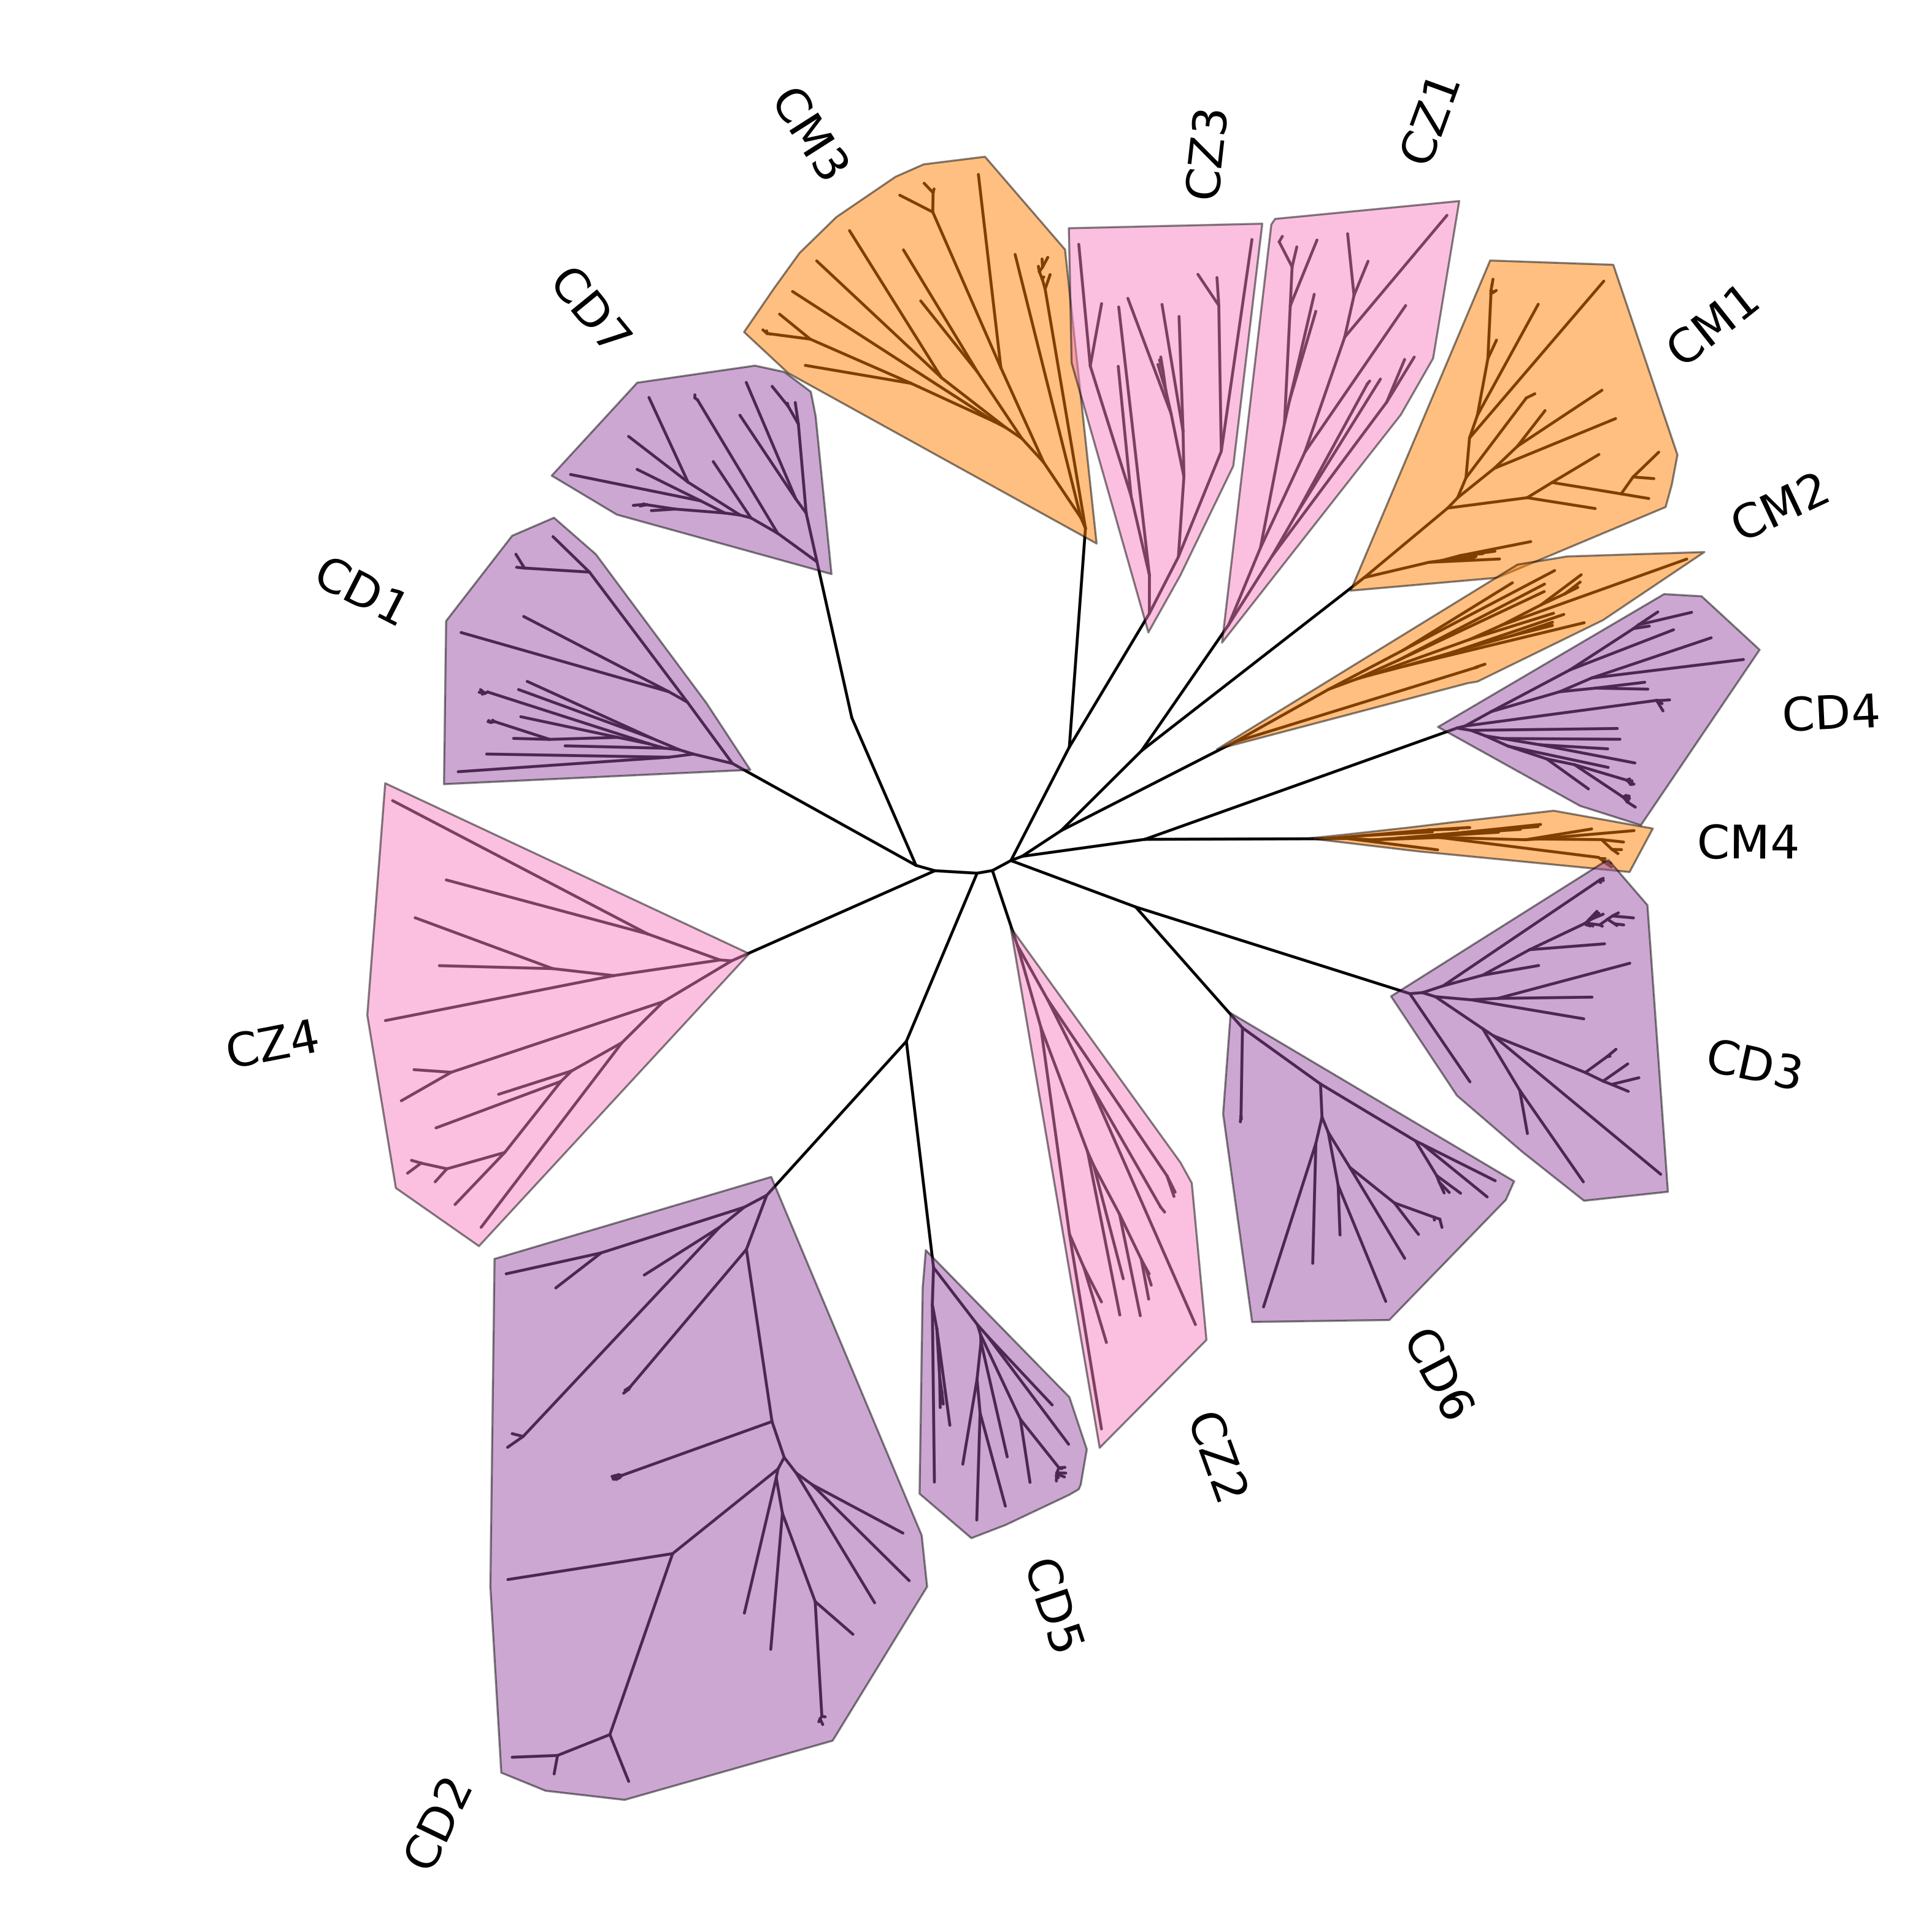
\includegraphics[width=0.9\textwidth]{_Figures/png/ch-tree-all}
\caption[\ch exons in the Atherinomorpha]{\textbf{\ch exons in the Atherinomorpha:} Unrooted phylogram of \ch exons in thirteen fish species from the Atherinomorpha, constructed using \program{PRANK} and \program{RAxML}. Each exon type is clustered separately in the tree topology, indicating that the types of the identified exons have all been correctly annotated.}
\label{fig:ch-tree-all}
\end{figure}

\begin{figure}
\centering
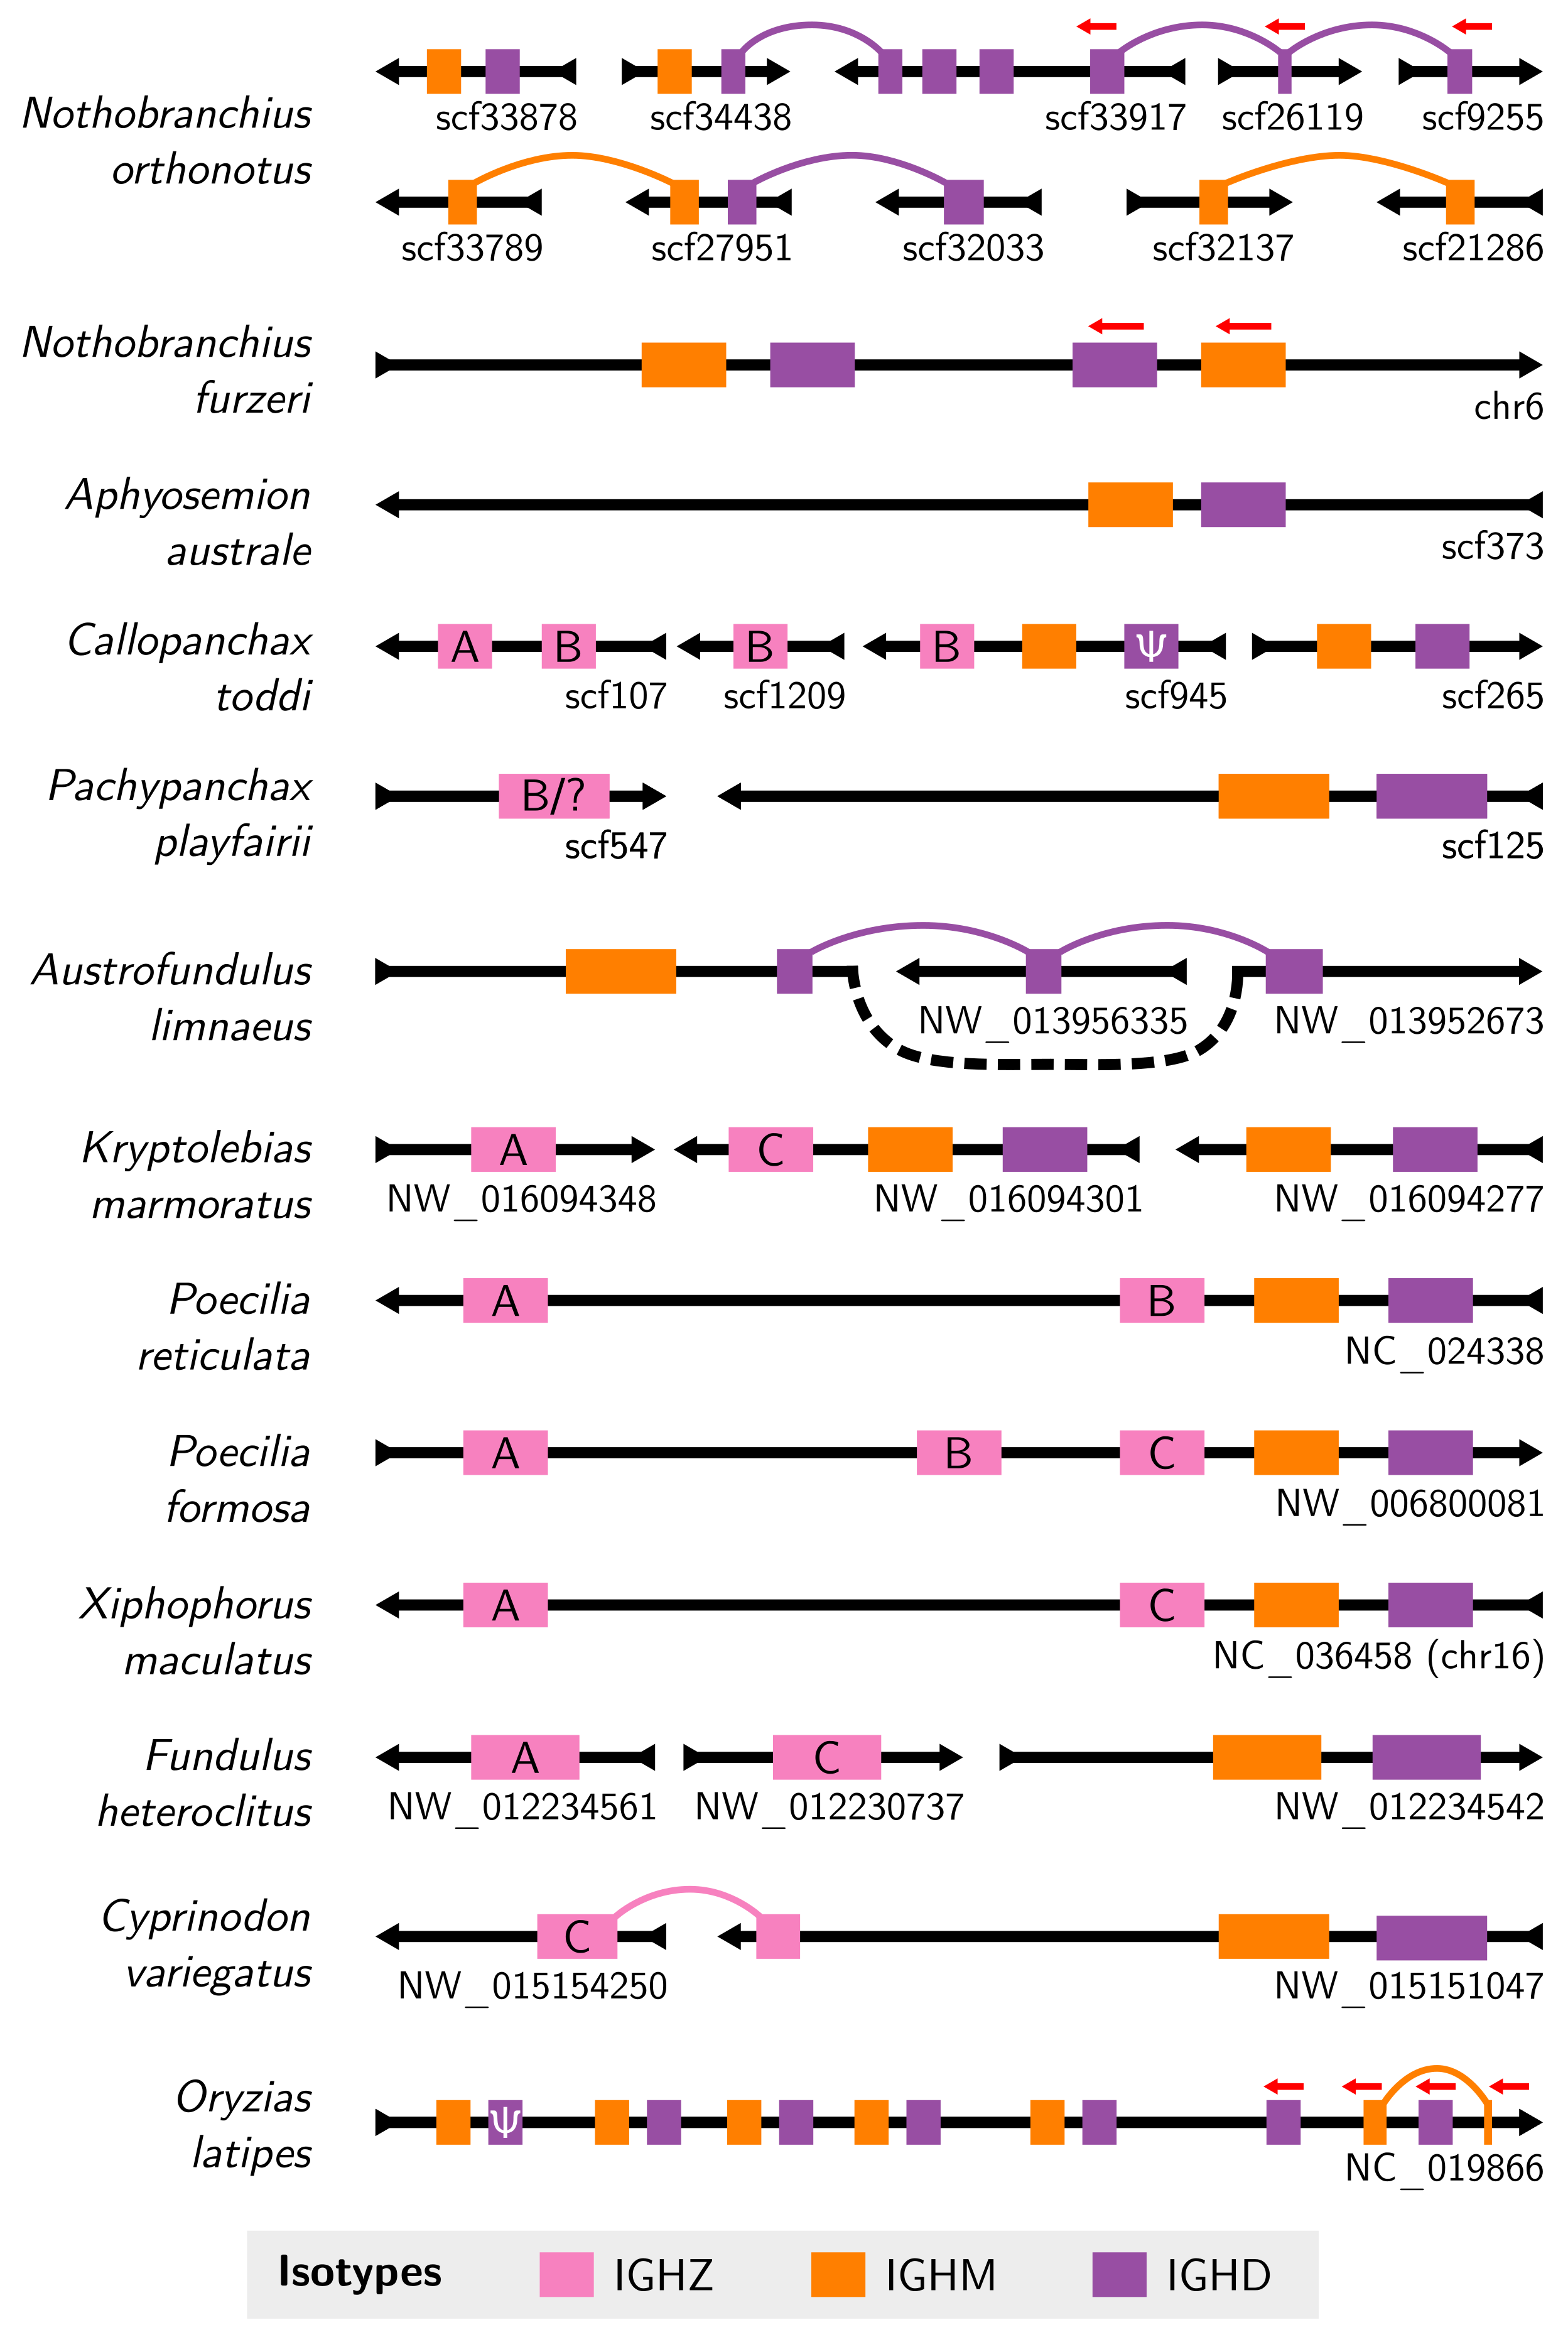
\includegraphics[width=0.9\textwidth]{_Figures/png_edited/multispecies-ch-regions}
\caption[Constant-region organisation in the Atherinomorpha]{\textbf{Constant-region organisation in the Atherinomorpha:}
Schematic of \igh{} constant regions in the genomes of thirteen species from the Atherinomorpha. Scaffold orientation is given by the black arrows; constant regions are oriented left-to-right unless otherwise specified (red arrows). Links between regions on different scaffolds indicate that exons from what appears to be the same constant region are distributed across multiple scaffolds in the order indicated; the order of unlinked scaffolds is arbitrary. The isotype of each region is given by its colour; \igh{Z} regions are further annotated with their subclass (\Cref{fig:species-tree-large-ighz}). Clearly pseudogenised constant regions are indicated by $\Psi$. Isotype length, scaffold length, and scaffold position are not to scale. Variable regions and lone, isolated constant-region exons are not shown.}
\label{fig:multispecies-ch-regions}
\end{figure}

In addition to at least one \igh{M} and \igh{D} constant region, the majority of species analysed (8 out of 13) were also found to possess at least one complete \igh{Z} constant region; of the exceptions, \species{A.}{limnaeus} exhibits an orphaned, pseudogenised \igh{Z-TM1} exon but no \cz exons in the current assembly (\Cref{fig:multispecies-ch-regions}, \Cref{tab:multispecies-ch-regions-2}), while \species{O.}{latipes}, \species{A.}{australe}, \Nfu and \species{N.}{orthonotus} display no \igh{Z} exons at all. Multiple duplications of \igh{Z} appeared even more common than for the other isotypes, with an average of 2.125 regions per \igh{Z}-bearing locus. Annotating the tree from \Cref{fig:species-tree-large-taxa} with the \igh{Z} status of each species (\Cref{fig:species-tree-large-ighz}) confirms that the loss of \igh{Z} in turquoise killifish (and related species) and medaka represent two distinct deletion events, with \textit{Austrofundulus limnaeus} potentially representing a third independent loss of \igh{Z} within the Atherinomorpha.

\begin{figure}
\centering
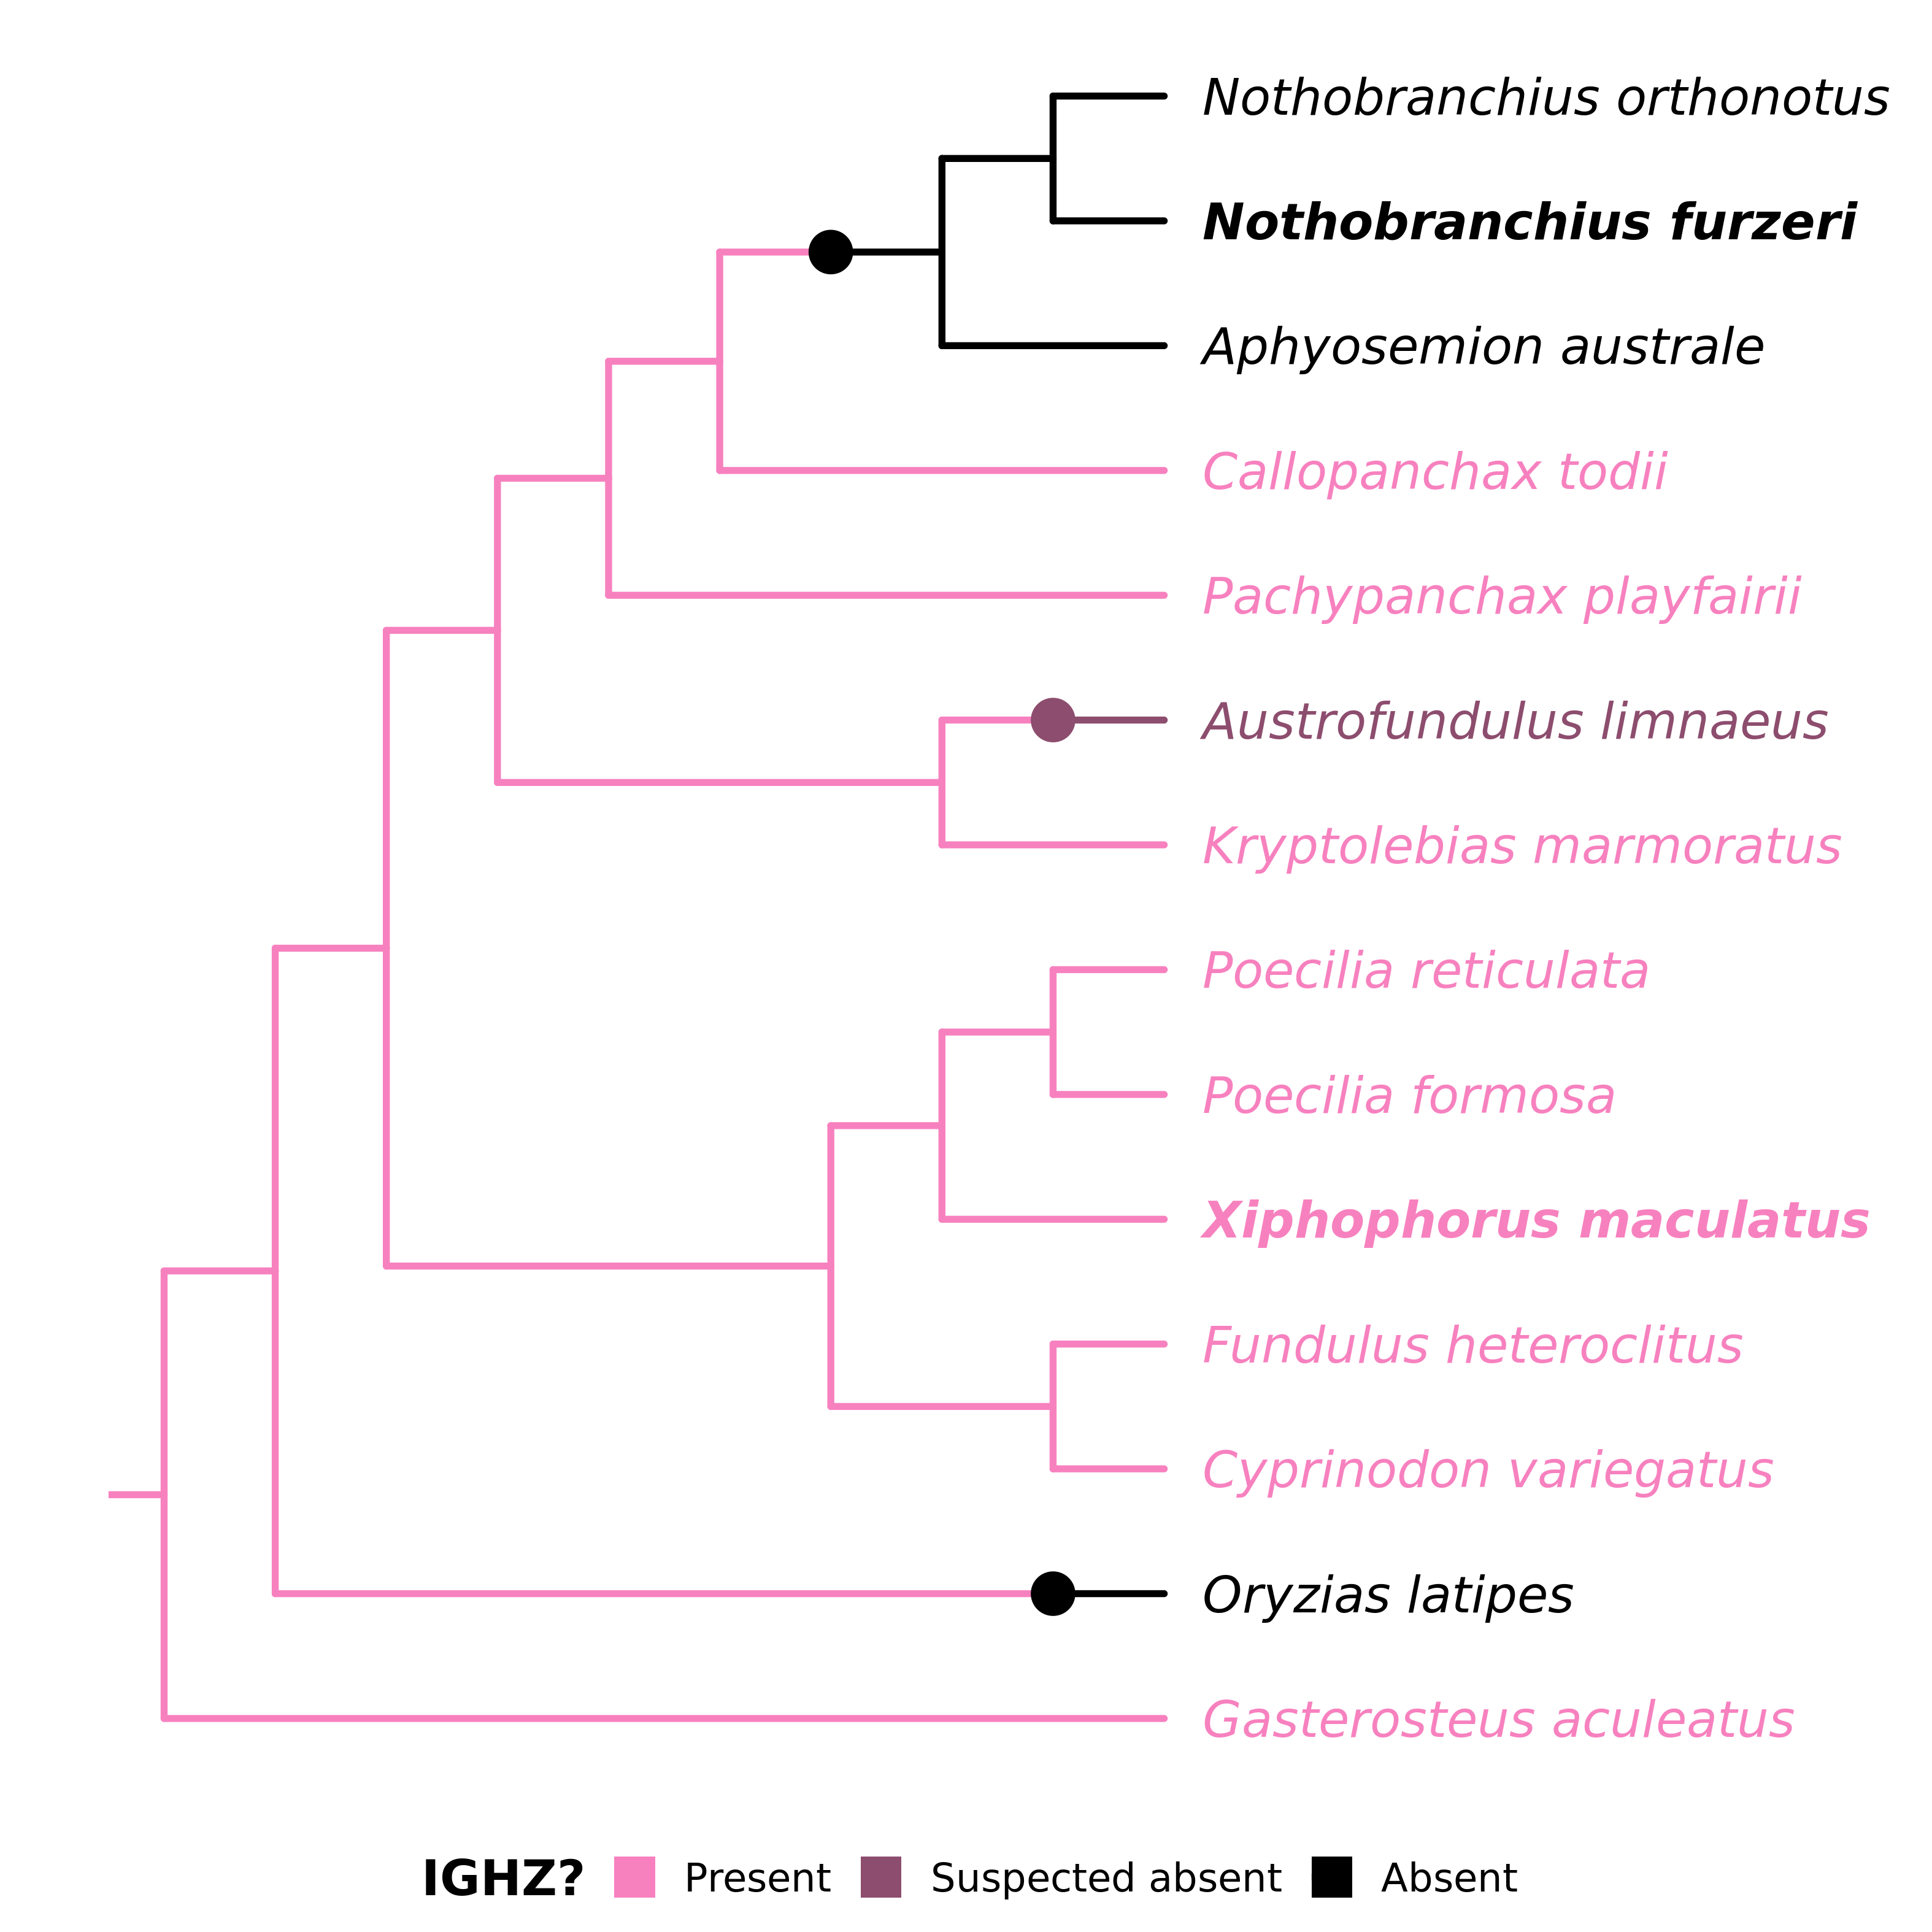
\includegraphics[width=0.9\textwidth]{_Figures/png/species-tree-large-ighz}
\caption[\igh{Z} in the Atherinomorpha has been lost multiple times independently]{\textbf{\igh{Z} in the Atherinomorpha has been lost multiple times independently:} Cladogram of species reproduced from \Cref{fig:species-tree-large-taxa}, annotated according to the known (tip nodes) or inferred (internal nodes) presence or absence of intact \igh{Z} constant regions in each species. Large coloured points on the cladogram denote sites of hypothesised state changes; \igh{Z} is assumed to be primitively present in the clade and losses to be irreversible. The currently-available genome assembly of \textit{A. limnaeus} (dark pink) contains one pseudogenised \igh{Z-TM1} exon and no \cz{} exons.}
\label{fig:species-tree-large-ighz}
\end{figure}

Apart from its repeated loss within the lineage, a second striking feature of \igh{Z} within the Atherinomorpha is its frequent presence in multiple copies per \igh{} locus; on average (geometric mean), the species analysed have approximately 1.62 \igh{Z} constant regions per \igh{M} constant region, and the same ratio veforrsus \igh{D}, suggesting a more complex evolutionary history than can be captured by a simple presence/absence metric. Concordantly, phylogenetic analysis (\Cref{fig:multispecies-cz-tree}, tree built using \program{PRANK} and \program{RAxML} on of \cz{1}--\cz{4} exon sequences) reveals three distinct lineages (or \textit{subclasses}) of \igh{Z} constant regions in the Cyprinidontiformes, each of which is present in multiple different species and appears to have been present in the common ancestor of the eight \igh{Z}-bearing species analysed (\Cref{fig:multispecies-cz-subclasses}).

\begin{figure}
	\centering
	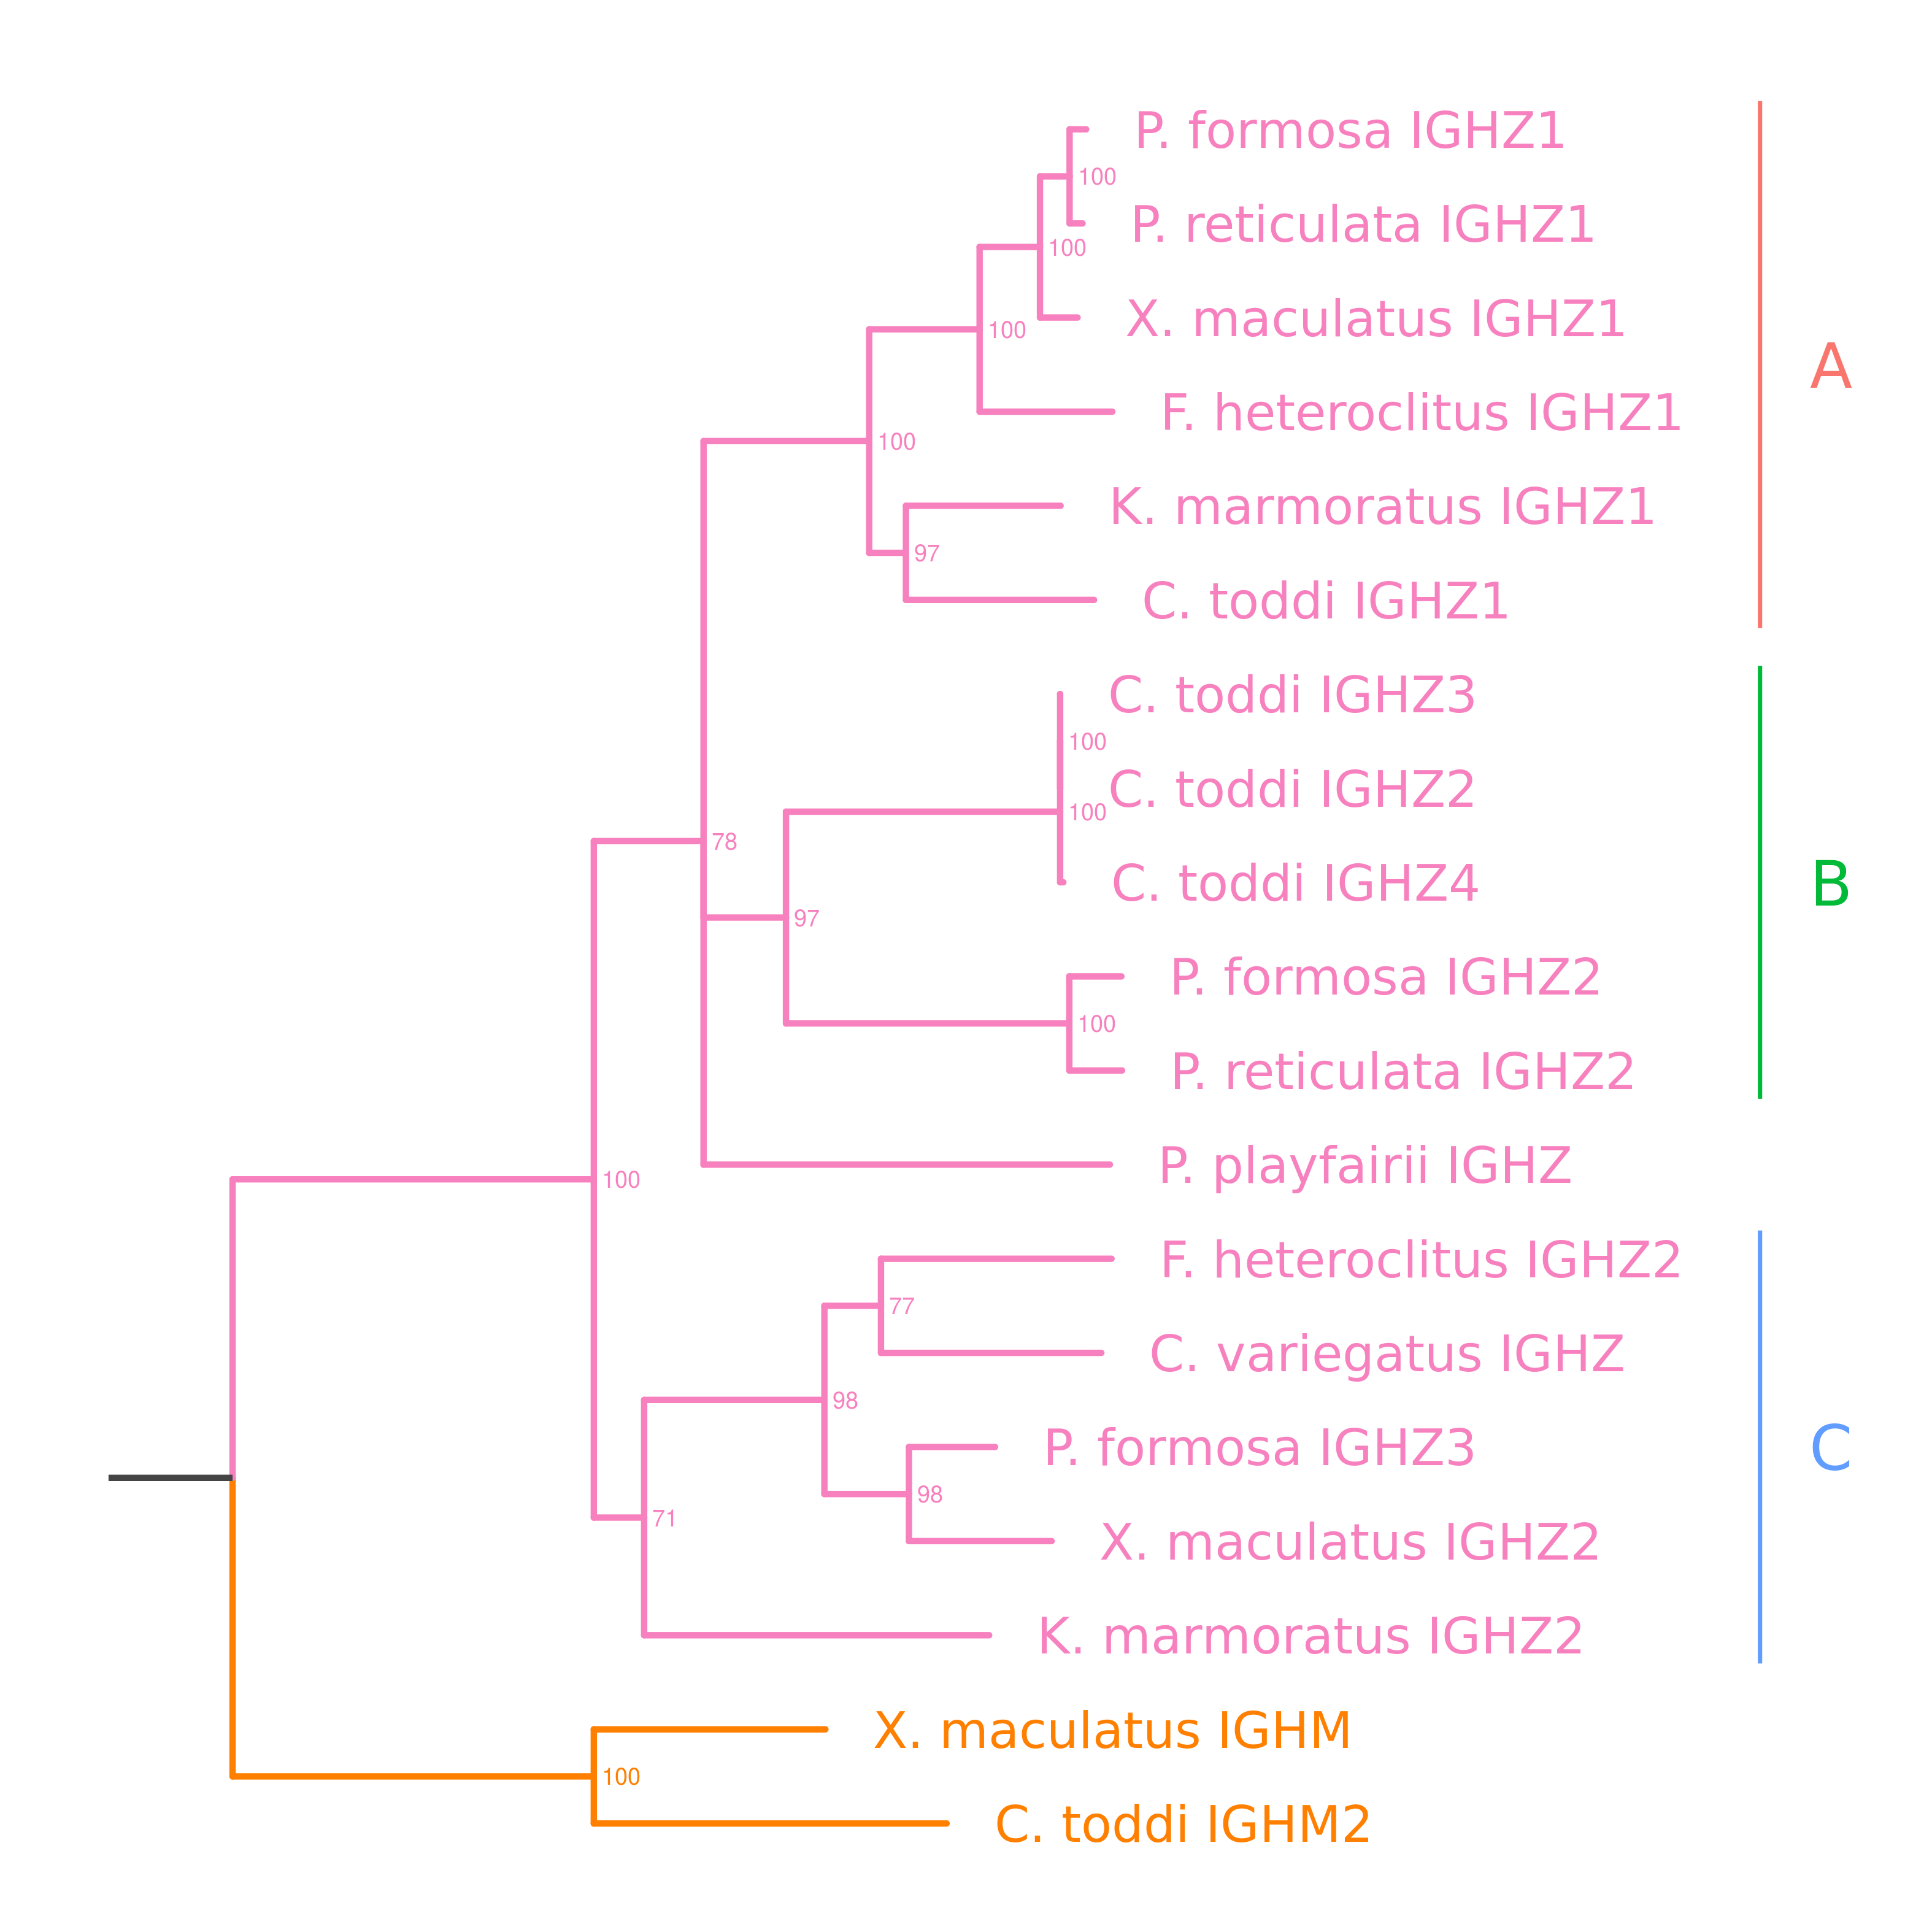
\includegraphics[width=0.9\textwidth]{_Figures/png/multispecies-cz-tree}
	\caption[\igh{Z} constant regions constitute three distinct subclasses]{\textbf{\igh{Z} constant regions constitute three distinct subclasses:} 
	Phylogram of concatenated \cz{1}--\cz{4} nucleotide sequences from \igh{Z}-bearing species in \Cref{tab:cyprinodontiform-genomes}, with \cm{1}--\cm{4} sequences from two species as an outgroup (in orange). Major clades (A--C) are annotated on the right. Support values indicate the result of rapid bootstrapping by \program{RAxML} across 1000 replicates.}
	\label{fig:multispecies-cz-tree}
\end{figure}

\begin{figure}
\centering
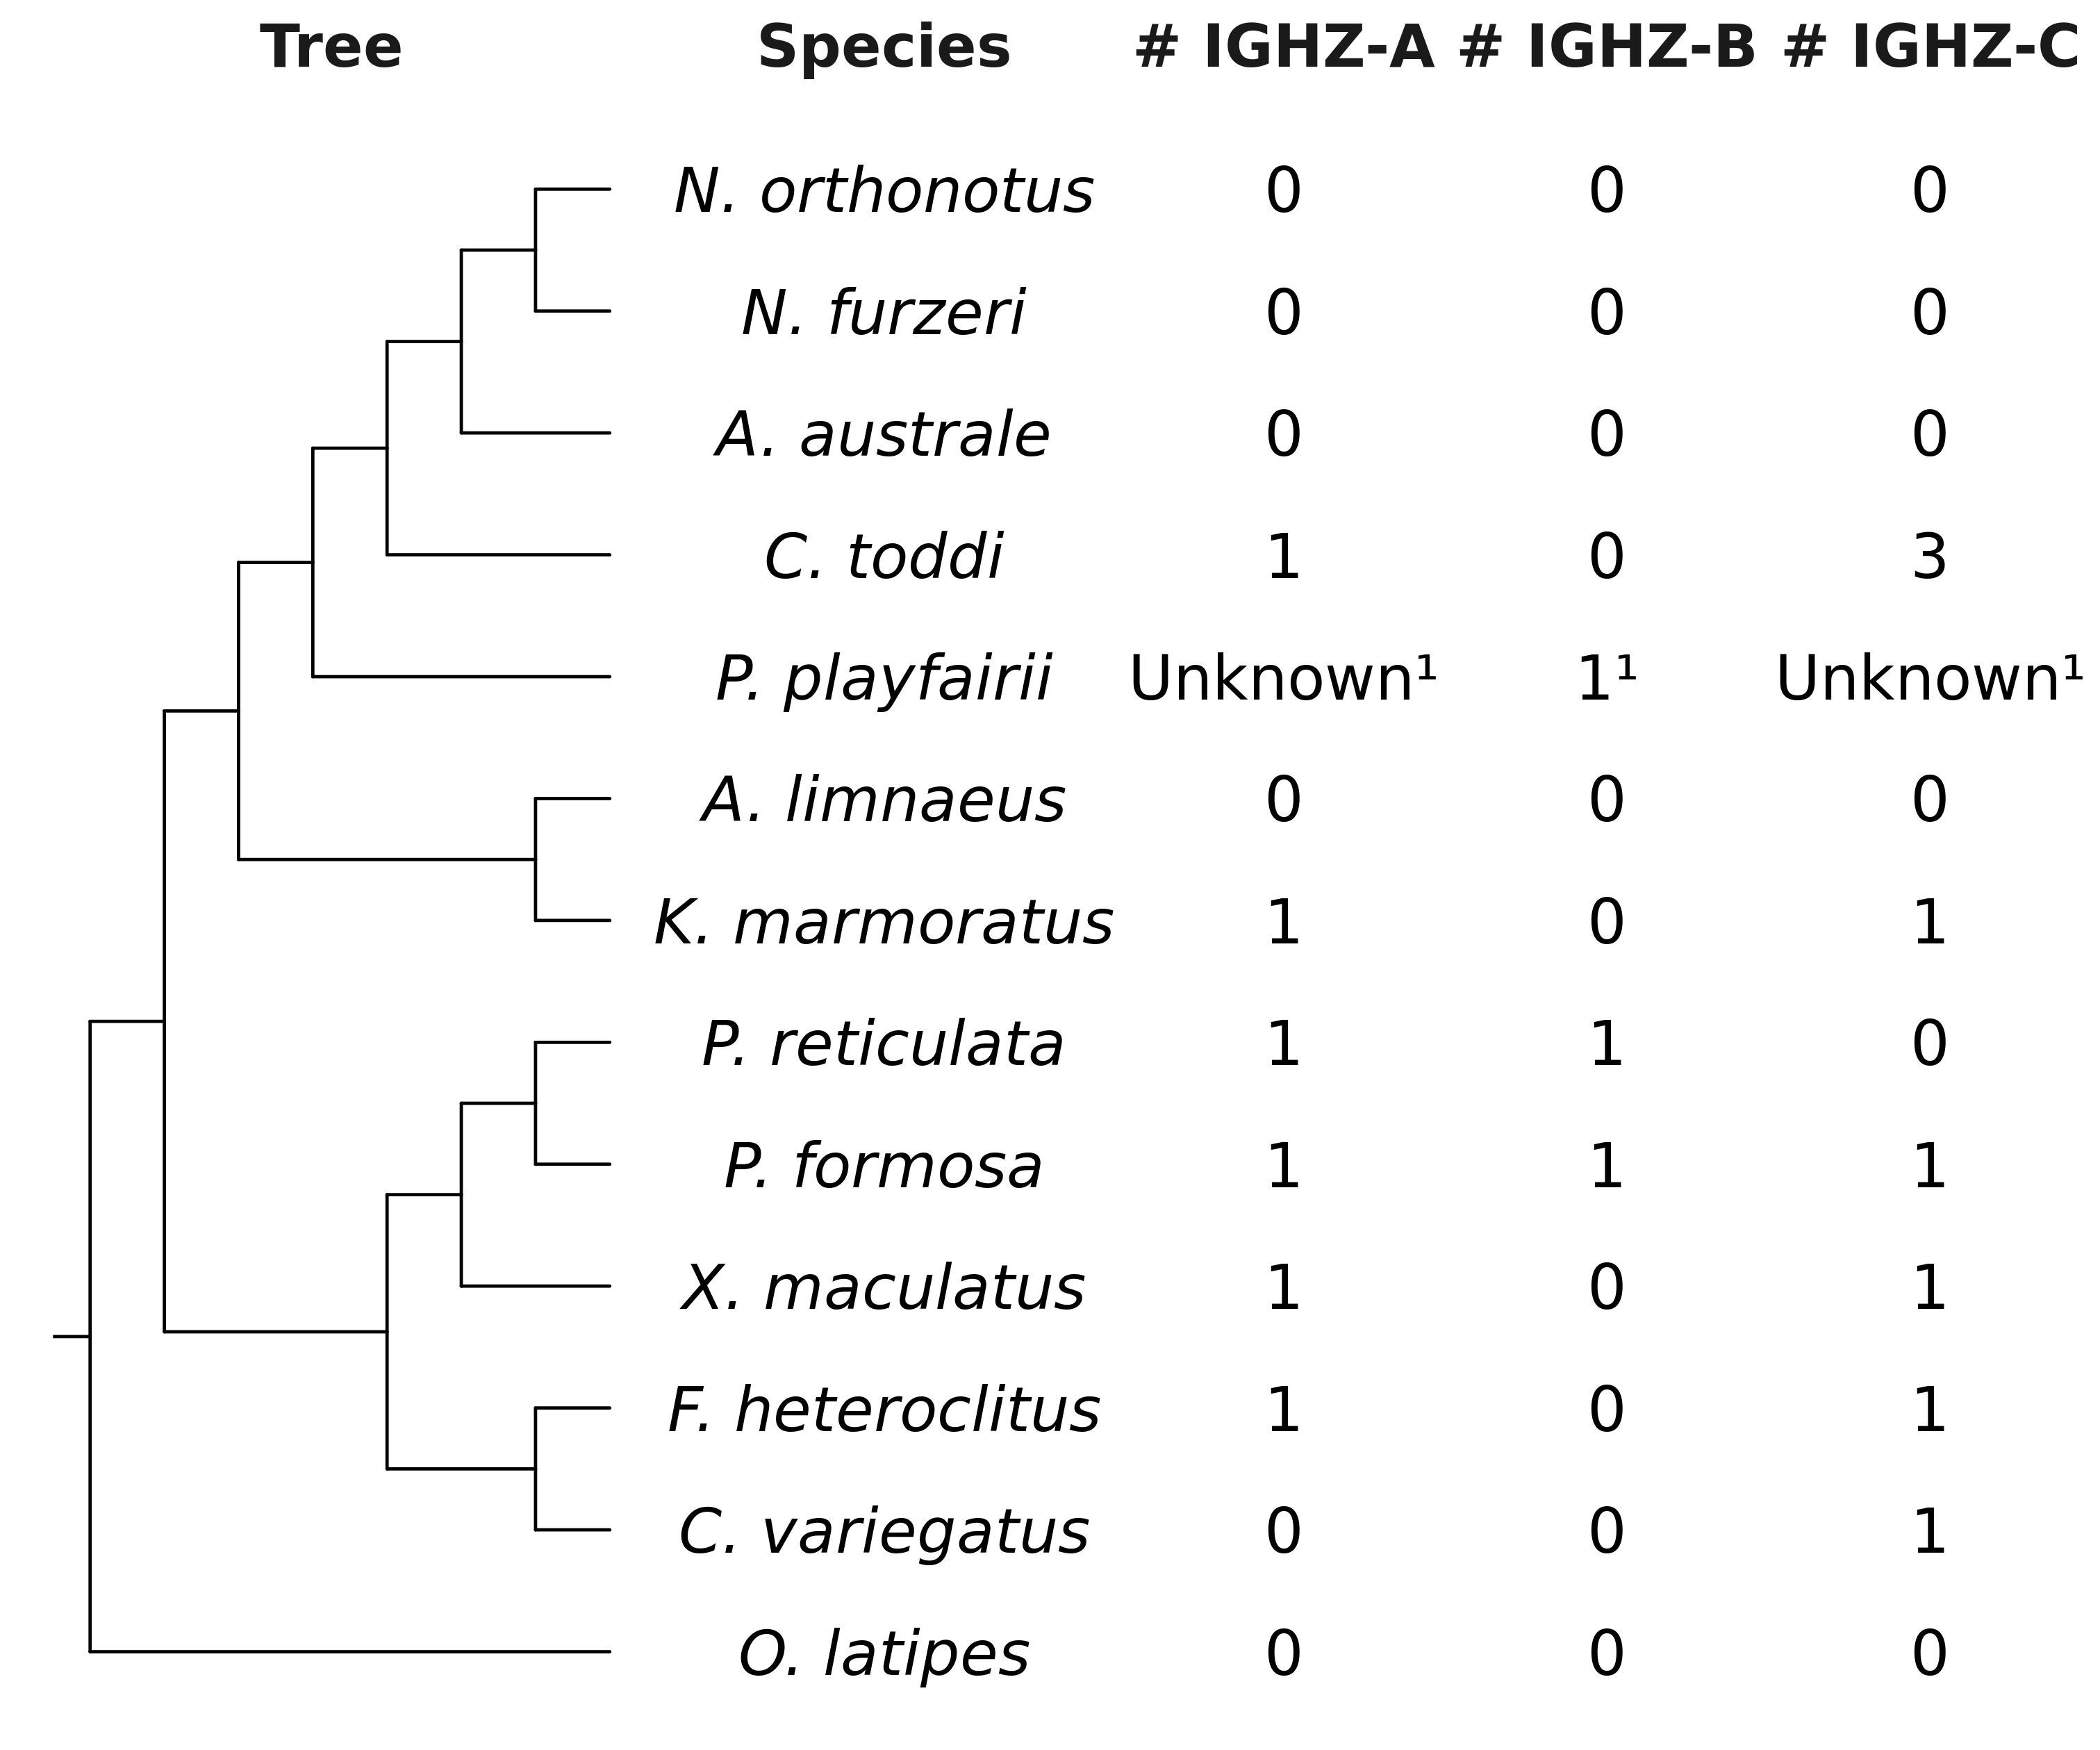
\includegraphics[width=0.8\textwidth]{_Figures/png/multispecies-cz-subclasses}
\begin{minipage}{0.7\textwidth}
\footnotesize
\begin{threeparttable}
\begin{tablenotes}
\item[1] \textit{P. playfairii} \igh{Z} \cz{1}--\cz{2} appear to be derived from \igh{Z-B}, while the other exons are of uncertain subclass origin (\Cref{fig:ppl-cz-aln}).
\end{tablenotes}
\end{threeparttable}
\end{minipage}
\caption[\igh{Z} subclasses in the Atherinomorpha]{\textbf{\igh{Z} subclasses in the Atherinomorpha:} Cladogram of atherinomorph species with characterised \igh{Z} constant regions, annotated with the number of regions belonging to each \igh{Z} isotype in each species. All three subclasses are present in at least one species in both major branches of the cyprinodontiform clade, suggesting that they were all present in the common ancestor of this grouping.}
\label{fig:multispecies-cz-subclasses}
\end{figure}


Only one \igh{Z} constant region from the analysed species could not be confidently assigned to one of these three subclasses, namely the single \igh{Z} of \species{Pachypanchax}{playfairii} (\Cref{fig:multispecies-cz-tree}). In order to more closely investigate the relationships of \igh{Z} in this species, the exon sequences of \species{P.}{playfairii} \cz{1}--\cz{4} were separately aligned to the \cz{} exons of all other \igh{Z}-bearing species using Needleman-Wunsch global alignments, and the distribution of alignment scores was plotted in \Cref{fig:ppl-cz-aln}
. The results show a striking difference in alignment behaviour between the exons, with \cz{1} and \cz{2} aligning much more strongly to exons from the B subclass and \cz{3} and \cz{4} showing more ambiguous affinity for either A- or C-subclass sequences. This unexpected behaviour indicates that the \species{P.}{playfairii} \igh{Z} sequence is the result of a deletion or fusion event combining the first two exons of a B-lineage \igh{Z} constant region with the latter exons of a constant region from another lineage, resulting in a chimeric gene with ambiguous ancestry.

\begin{figure}
	\centering
	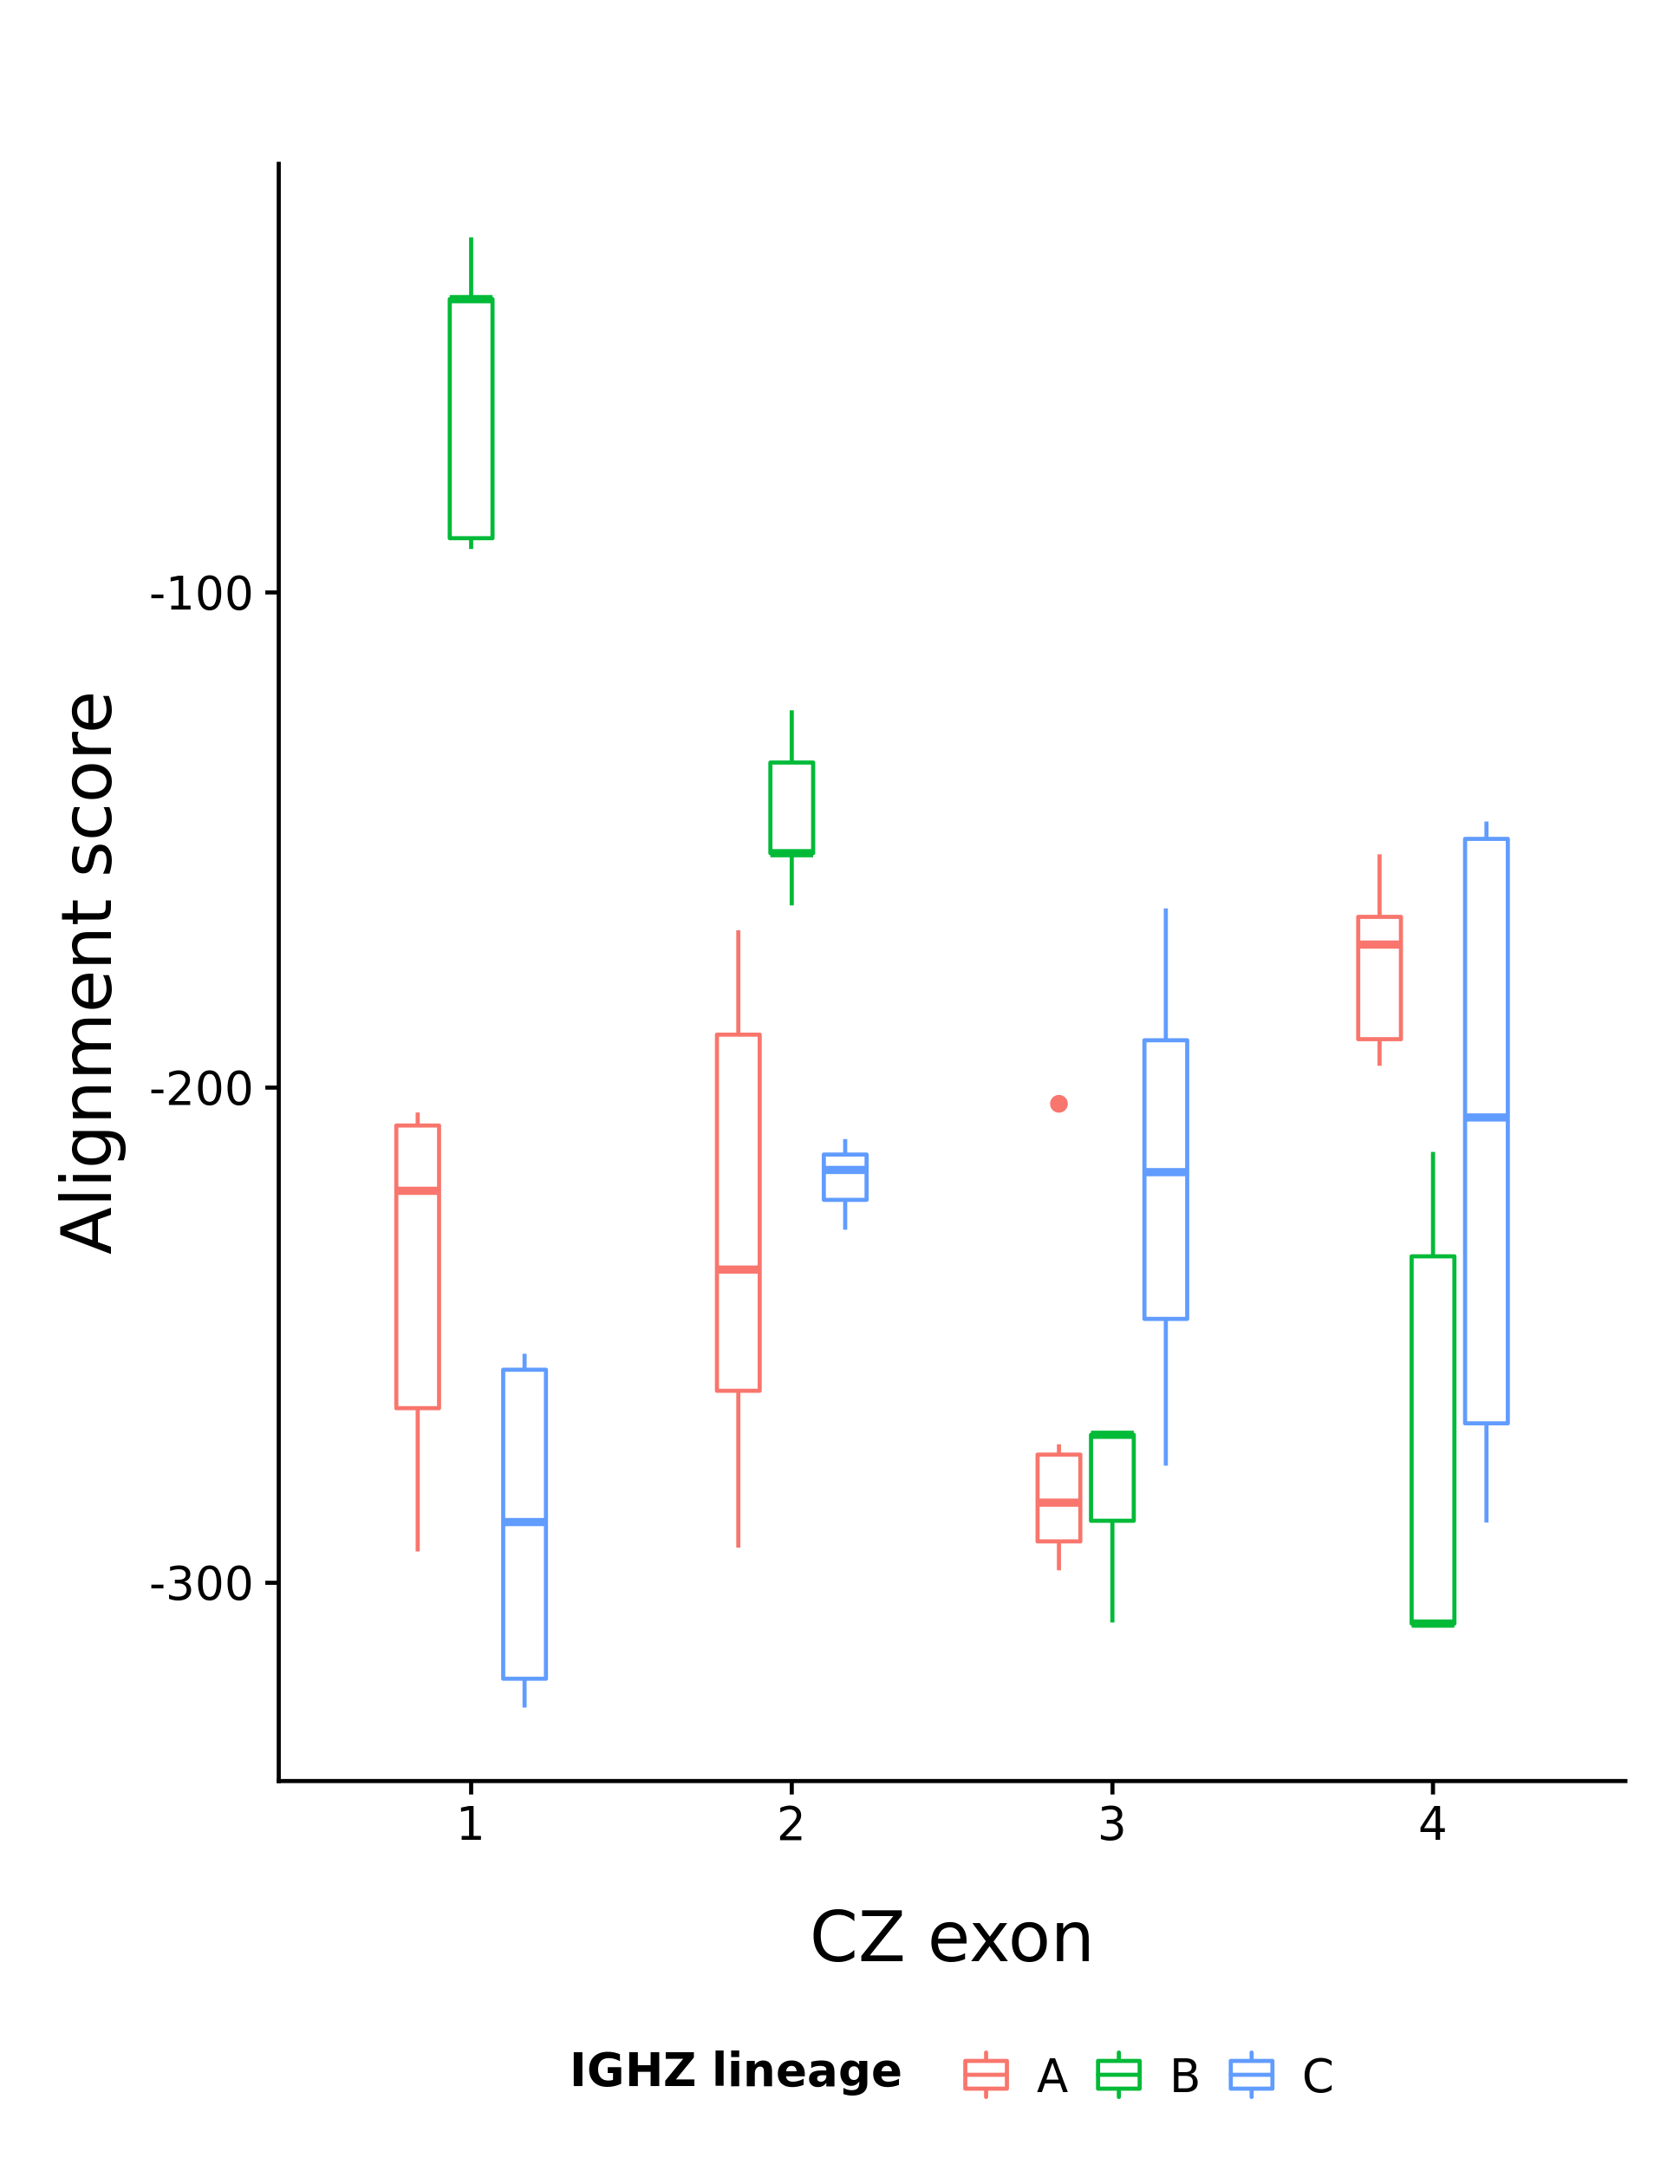
\includegraphics[width=0.7\textwidth]{_Figures/png/ppl-cz-aln-aa.png}
	\caption[Subclass affinity of \species{Pachypanchax}{playfairii} \igh{Z}]{\textbf{Subclass affinity of \species{Pachypanchax}{playfairii} \igh{Z}:} 
	Boxplots of Needleman-Wunsch alignment scores between the amino-acid sequences of \species{P.}{playfairii} \cz{} exons and those of seven other \igh{Z}-bearing cyprinodontiform species, demonstrating the differing affinity of diferent \species{P.}{playfairii} exons for each of the three \igh{Z} subclasses.}
	\label{fig:ppl-cz-aln}
\end{figure}
	
In summary, in addition to the still-universal primitive antibody classes \igh{M} and \igh{D}, the cyprinodontiforms ancestrally possessed both at least three variants of \igh{Z}, giving rise to multiple subclasses of \igh{Z} constant regions evolving in parallel across the clade. Each of these subclasses appears to have been lost in multiple cyprinodontiform species, with different species showing distinct patterns of retention and loss, and in at least one lineage -- that of \species{Pachypanchax}{playfairii} -- two different \igh{Z} lineages have fused to produce a chimeric isotype. All three subclasses are missing from a subset of species in the Nothobranchiidae (including \nfu), and also appear to have been independently lost in \species{Austrofundulus}{limnaeus}. Taken together, these data suggest a high degree of complexity and volatility in the evolution of mucosal adaptive immunity in the Cyprinodontiformes.


	% Discussion

	%	The examination of the constant-region structures present in the \Xma IGH locus therefore reveals three notable features that differ in state between medaka, turquoise killifish, and the southern platyfish. Most strikingly, the absence of IGHM in medaka and killifish, but its presence in platyfish, strongly suggests that the isoform has been lost independently in the two groups. Conversely, the presence of a four-exon IGHM-TM in medaka and killifish, but a five-exon configuration in platyfish, is less clear-cut: it may indicate an independent change in medaka and killifish that is absent in platyfish, but may also plausibly represent a reversion in platyfish to the more-primitive five-exon state. Without a deeper understanding of the currently-unknown physical underpinnings of this observed difference in splicing behaviour, this question can only be addressed through analysis of RNA-seq data from a large number of related species, something beyond the scope of the present investigation. % TODO: Do it anyway?
%	Finally, the presence of a (\cd{2}-\cd{3}-\cd{4}) duplication in both platyfish and killifish, but not in medaka, suggests that this may be a shared primitive feature of the Cyprinodontiforms; however, given the apparent recurrence of this duplication pattern in many different groups across the teleosts, a strong conclusion cannot be drawn without a higher-resolution phylogenetic analysis of a larger number of related species.
% TODO: Move to multispecies section intro

	%	TODO: Move to multilocus section. Alongside this, I performed a more limited characterisation of the \textit{IgH} constant regions in 9 %?
%	additional cyprinodontiform and beloniform species, to assess the broader patterns of immunoglobulin heavy chain evolution within these groups (\Cref{sec:comparative-loci}). The results of these additional investigations repeatedly called into question the hypothesis of homology in IgH locus ideosyncracies between medaka and turquoise killifish, and suggest a model of rapid locus evolution within this diverse and important teleost clade.
	
	% TODO: Move to discussion section.
	% TODO: Relationship between killifish Vs and other species
	% TODO: Evolution of IGH1 vs 2
	% TODO: Discussion of mucosal immunity in absence of IGZ
		% TODO: Discuss smallness of killifish locus in the context of relaxed purifying selection and short life span
	% TODO: Section on "Investigating the evolutionary relationship between IGH1 and IGH2"
	% Keep for discussion:
%\q{Given the lack of IgZ in this species, how do you think they carry out mucosal immunity?}
%
%I'd assume using IgM. It's the primitive antibody and is expressed in secreted form in the killifish gut. I haven't investigated the protein expression so it's hard to say for sure, but I'd guess that's the answer. It's also quite possible, lacking a specialised mucosal class, that the answer is ``not very well". It would be very interesting to compare mucosal immune function in species with and without IgZ, especially if those species are closely related.
%
%Given the impressive results indicating the specificity of IgT for mucosal immunity in trout, and the lack of mucosal response of IgM in that species, it would be very interesting to see what mucosal responses look like in a species that lacks that isotype -- is IgM much more responsive and expressed in the gut than in IgT-possessing species, or is the mucosal response just worse?
	% (Incidentally, it would be great to see whether any B-cells in TK show recombinations in both subloci, vs one or the other. Single-cell DNA sequencing could plausibly do this.)

%	The specialised mucosal isotype \igh{Z} is present in the majority of teleost \igh{} loci characterised so far, including several species (including stickleback and fugu) relatively closely related to the Atherinomorpha; the possession of \igh{Z} therefore appears to be primitive to most groups of teleost fish. The striking absence of the isotype in both medaka and turquoise killifish (\Cref{sec:nfu-locus-constant}), the first two characterised \igh{} loci from the Atherinomorpha, suggested that the lack of \igh{Z} may have occurred in the common ancestor of both species and so be primitive both the Beloniformes and Cyprinodontiformes; however, the surprising presence of two distinct \igh{Z} loci in the locus of the southern platyfish \xma convincingly falsified this hypothesis and indicated that the loss of \igh{Z} in medaka and turquoise killifish occurred independently in their respective lineages (\Cref{sec:xma-locus-constant}). % TODO: For discussion
% It is not known whether these subclasses have distinct functional properties, or how these % TODO: For discussion








	





%%!TEX root = ../thesis.tex

\chapter{Materials and Methods}
%s\doublespacing
\onehalfspacing


%
%\ifpdf
%    \graphicspath{{Chapter1/Figs/Raster/}{Chapter1/Figs/PDF/}{Chapter1/Figs/}}
%\else
%    \graphicspath{{Chapter1/Figs/Vector/}{Chapter1/Figs/}}
%\fi

\section*{Summary} % Fits one one page if 1.5-spaced, but not at double spacing

% ...
\pagebreak

%...

\section{Characterising the killifish \textit{IgH} locus}

% ...

\subsection{Assembling BAC inserts from Illumina reads}

The data from the BAC sequencing runs were trimmed of adaptor sequences by the sequence provider and uploaded to Illumina Basespace %trademark? citation
for online storage and sharing. These data were downloaded from BaseSpace to our institute file server with Illumina BaseMount % trademark? citation?
and uploaded to the institute computing cluster with SCP. % citation
Information about these raw sequencing libraries can be found in Table\dots %TODO: Add BAC info table
. 

The general outline of the BAC assembly pipeline used in this work is shown in Figure\dots %TODO: Make BAP flowchart figure
. In brief, the input reads were trimmed to remove low-quality bases using Trimmomatic; filtered using Bowtie2 to remove contaminant sequences; assembled into contigs using the SPAdes genome assembler; then scaffolded using BESST and long-insert libraries from the killifish genome project. % Citations for all of this
Each of these stages is described in more detail below; the complete pipeline is available at \dots .

\subsubsection{Quality-trimming with Trimmomatic}

Quality trimming to remove low-quality and adaptor sequences is important for the performance of \textit{de novo} sequence assembly applications \citep{bolger2014trimmomatic}, potentially yielding large gains in assembly quality. In this project, the widely-used quality-trimming tool Trimmomatic \citep{bolger2014trimmomatic} was used to process all BAC reads prior to filtering and assembly. Trimmomatic is capable of processing single- or paired-end read data, but its adaptor-removal performance is substantially higher when pairing information is available; it was therefore run on paired read data, before the files were split for contamination filtering (see below). The command used ((for Illumina data)) was:

ILLUMINACLIP:<path_to_adapters>:2:30:10:5:true LEADING:20 TRAILING:20 SLIDINGWINDOW:4:30 MINLEN:36 % TODO: Format this properly

Which applies the following operations (in order):

\begin{itemize}
\item ILLUMINACLIP: Scan reads for Illumina adapter sequences (using both simple and palindromic search modes \citep{bolger2014trimmomatic}) and remove them. The "true" option instructs Trimmomatic to retain both reads in the event that they are identical after adapter-trimming.
\item LEADING: Remove bases below the stated quality threshold from the start of the read.
\item TRAILING: Remove bases below the stated quality threshold from the end of the read.
\item SLIDINGWINDOW: Trim reads if the average quality score across a sliding window drops below a threshold value
\item MINLEN: Discard reads below some threshold length (post-trimming)
\end{itemize}

% Talk about TruSeq vs NextEra adaptor selection (if both, then why?)

\subsubsection{Contaminant-filtering with Bowtie2}

The presence of contaminating sequences in the read set can significantly impair \textit{de novo} sequence assembly, resulting in both contamination of the resulting assembly and a reduction in the length and reliability of true contigs %citation needed
. To avoid this, stringent filtering is required to remove reads aligning to expected contaminant sequences. In this case, observed contaminants included:

\begin{itemize}
\item Genomic DNA \textit{Escherichia coli} strain K12/DH10B (the strain of \textit{E. coli} used in the BAC library) % Other strains?
\item Fragments of genomic DNA from \textit{Amycolatopsis lurida} % More info - what gene if any, why is it there
\item Low levels of \textit{Homo sapiens} sequences
\end{itemize}

To remove these, the relevant sequences (see Table ((?)) ) were used to construct an index for the widely-used read-mapping program Bowtie2 \citep{langmead2012bowtie2},
, and the trimmed reads were aligned against this index. 


To maximise stringency, the forward and reverse reads files were each aligned separately, with reads that failed to align (i.e. that did not contain contaminating sequence) output to a new file with Bowtie2's --un argument; reads that did align to the contaminating sequences were discarded % Insert command here

Among those reads showing significant alignment to the reference sequence, some aligned concordantly (with both reads aligning to the contaminating sequence in a consistent manner) and others discordantly (with only one read aligning or the two reads aligning in a manner inconsistent with the sequencing format). In order to maximise stringency, any read pair in which at least one read aligned to a contamination sequence was deemed to be contaminated and removed from the read set prior to sequence assembly. To achieve this, the forward and reverse reads files were each aligned to the contamination index separately, with reads that failed to align (i.e. that did not contain contaminating sequence) output to a new file with Bowtie2's --un argument; reads that did show significant alignment to the reference sequence were discarded. % Insert command here

The forward and reverse read files were then re-synchronised using the re-pairing tool `rpair.sh` from the BBTools suite % no citation - link to website?
, which identifies paired reads using standard Illumina formatting conventions, discards reads with no pair in the other file and reorders the files so that paired reads are at corresponding positions. As a result of this last pre-processing step, only read pairs in which both partners failed to align to the contamination index were retained for sequence assembly.

\subsubsection{BAC sequence assembly with SPAdes}

Following quality-trimming and filtering of contaminating sequences, the remaining BAC reads underwent \textit{de novo} genome assembly using the de-Bruijn-graph-based assembly software SPAdes \citep{bankevich2012spades}. SPAdes is specialised for assembling small genomes and utilises... %Re-read the paper
including sophisticated error correction with the built-in correction utility BayesHammer \citep{nikolenko2013bayeshammer}. Standard parameters for assembling 250+bp MiSeq reads were used as recommended by the developers % cite website
; in particular, k-mer sizes of %...
were used in the iterated assembly.

% Command here

Following conclusion of the SPAdes pipeline, the initial BAC assemblies were assessed  (both individually and all together) using the widely-used quality-assessment tool QUAST % Citation here...

\subsubsection{Scaffold assembly with BESST}

As the insert sequences of the killifish BAC library were drawn from the killifish genome, long-insert read libraries used in the killifish genome project could be used to improve the quality of the BAC assemblies.

To achieve this, the SPAdes assemblies
with the scaffolding program BESST \citep{sahlin2014besst}.

\section{Analysis of IgSeq data}

\subsection{Pre-processing with pRESTO}

\subsection{


%\include{B_Chapters/Chapter3/chapter3}
%\include{B_Chapters/Chapter4/chapter4}
%\include{B_Chapters/Chapter5/chapter5}
%\include{B_Chapters/Chapter6/chapter6}
%\include{B_Chapters/Chapter7/chapter7}
%\include{Chapter8/chapter8}
%


% ********************************** Back Matter *******************************
% Backmatter should be commented out, if you are using appendices after References
%\backmatter

% ********************************** Bibliography ******************************
\begin{spacing}{0.9}

% To use the conventional natbib style referencing
% Bibliography style previews: http://nodonn.tipido.net/bibstyle.php
% Reference styles: http://sites.stat.psu.edu/~surajit/present/bib.htm

%\bibliographystyle{apalike}
\bibliographystyle{unsrt} % Use for unsorted references 
% TODO: Fix bibliography style 
%\bibliographystyle{plainnat} % use this to have URLs listed in References
%\cleardoublepage
%\bibliography{D_References/igh-locus} % Path to your References.bib file
\bibliography{D_References/Locus} % Path to your References.bib file

% If you would like to use BibLaTeX for your references, pass `custombib' as
% an option in the document class. The location of 'reference.bib' should be
% specified in the preamble.tex file in the custombib section.
% Comment out the lines related to natbib above and uncomment the following line.

%\printbibliography[heading=bibintoc, title={References}]


\end{spacing}

% ********************************** Appendices ********************************

\begin{appendices} % Using appendices environment for more functionality
\appendix
\chapter{Solutions and buffers}
\label{app:solutions}
\footnotesize
\section{Enzymes}
\label{app:solutions_enzymes}

\begin{threeparttable}
\begin{tabular}{lccc}\toprule
\textbf{Enzyme} & \textbf{Concentration} & \textbf{Manufacturer} & \textbf{Product code} \\\midrule
KAPA HiFi HotStart ReadyMix PCR Kit & \x{2}\tnote{a} & Kapa Biosystems & KR0370 \\
SMARTScribe Reverse Transcriptase & \unitsul{100} & Clontech Laboratories & 639537 \\
RNasin RNase inhibitor & \unitsul{40} & Promega &  N2511 \\
Uracil DNA glycosylase (UDG) & \unitsul{5} & NEB & M0280S \\
RNase A & \mgml{100} & QIAGEN & 19101 \\
\bottomrule \end{tabular}
\begin{tablenotes}
\item[a] KAPA HiFi HotStart DNA Polymerase present at \unitsul{0.04}.
\end{tablenotes}
\end{threeparttable}

\section{Non-enzyme reagents and components}
\label{app:solutions_reagents}

{\renewcommand{\arraystretch}{1.2}
\begin{threeparttable}
\begin{tabular}{lccc}\toprule
\textbf{Reagent} & \textbf{Concentration} & \textbf{Manufacturer} & \textbf{Product code} \\\midrule
SMARTScribe first-strand buffer & \x{5} & Clontech Laboratories & 639537\tnote{a}\\
Dithiothreitol (DTT) & \mmol{20} & Clontech Laboratories & 639537\tnote{a}\\
dNTP mix & \umol{10} each\tnote{b} & NEB & N0447L \\
\um{1} Sera-Mag™ Magnetic SpeedBeads™ & \mgml{50} & GE Healthcare & 65152105050250\\
QIAzol Lysis Reagent & \x{1} & QIAGEN & 79306\\
BluePippin electrophoresis buffer & \x{1} & Sage Science &BDF1510\tnote{c}\\
BluePippin R2 loading solution / marker mix & \x{1} & Sage Science &BDF1510\tnote{c}\\
Roti-Phenol/chloroform/isoamyl alcohol & \x{1} & Roth & A156.2\\
\bottomrule \end{tabular}
\begin{tablenotes}
\item[a] Supplied with SMARTScribe Reverse Transcriptase (\Cref{app:solutions_enzymes}).
\item[b] i.e. \umol{10} each of dATP, dGTP, dCTP and dTTP.
\item[c] Supplied with BluePippin \pc{1.5} agarose dye-free cassettes.
\end{tablenotes}
\end{threeparttable}
}

\section{Prepared buffers}
\label{app:solutions_buffers}
\begin{threeparttable}
\begin{tabular}{cllcc}\toprule
\textbf{Name} & \textbf{Purpose} & \textbf{Composition} & \textbf{\ph{}} & \textbf{Storage (\degC{})}\\\midrule
TET & Washing SeraMag beads & ~~\llap{\textbullet}~~ \mmol{10} Tris base & 8.0\tnote{a} & RT \\
& & ~~\llap{\textbullet}~~ \mmol{1} Na\textsubscript{2}-EDTA & & \\
& & ~~\llap{\textbullet}~~ \pc{0.05} (v/v) Tween 20 & & \\\midrule
iSB & Preparing SeraSure bead suspension & ~~\llap{\textbullet}~~ \mol{4.2} NaCl & 8.0\tnote{a} & RT \\
& & ~~\llap{\textbullet}~~ \mmol{16.8} Tris base & & \\
& & ~~\llap{\textbullet}~~ \mmol{1.68} Na\textsubscript{2}-EDTA & & \\\midrule
EB & Buffering nucleic-acid solutions & ~~\llap{\textbullet}~~ \mmol{10} Tris-HCl & 8.5\tnote{a} & RT \\\midrule
P1 & Resuspending cultured \textit{E. coli} cells & ~~\llap{\textbullet}~~ \mmol{50} Tris-HCl}& 8\tnote{a} & 4\tnote{c} \\
& & ~~\llap{\textbullet}~~ \mmol{10} Na\textsubscript{2}-EDTA & & \\
& & ~~\llap{\textbullet}~~ \ugml{100} RNase-A\tnote{b} & & \\\midrule
P2 & Cell lysis & ~~\llap{\textbullet}~~ \mmol{200} Sodium hydroxide & -- & RT \\
& & ~~\llap{\textbullet}~~ \pc{1} (v/v) Sodium dodecyl sulfate & & \\\midrule
P3 & Precipitation of cell lysate & ~~\llap{\textbullet}~~ \mol{3} Potassium acetate & 5.5\tnote{d} & RT \\\midrule
\end{tabular}
\begin{tablenotes}
\item[a] Adjust to the required \ph{} with hydrochloric acid (HCl).
\item[b] \Cref{app:solutions_enzymes}.
\item[c] Can be stored at room temperature before addition of RNase-A.
\item[d] Adjust to the required \ph{} with glacial acetic acid.
\end{tablenotes}
\end{threeparttable}
%\afterpage{\begin{landscape}

\chapter{Primers and oligonucleotides}
\label{app:oligos}

\section{Template-switch adapter oligos for reverse transcription}
\label{app:oligos_tsa}

\begin{threeparttable}
\begin{tabular}{cp{11cm}cc}\toprule
\textbf{Name} & \textbf{Sequence} & \textbf{Source} \\\midrule
SmartNNNa & AAGCAGUGGTAUCAACGCAGAGUNNNNUNNNNUNNNNUCTTrGrGrGrG & \parencite{turchaninova2016igprep}\\
\bottomrule
\end{tabular}
\end{threeparttable}

\section{PCR and reverse-transcription primers}
\label{app:oligos_primers}

\begin{threeparttable}
\begin{tabular}{cp{7cm}cccc}\toprule
\textbf{Name} & \textbf{Sequence} & \textbf{Purpose} & \textbf{Source}\tnote{a} \\\midrule
RT1 & TGGTCTTGCCAGCTGGTGATTTCCGCC & \igseq \cm{2} RT\tnote{b}~primer & -- \\\midrule
M1SS & AAGCAGTGGTATCAACGCA & \igseq PCR1 forward primer & \parencite{turchaninova2016igprep} \\
IGH-B & CCACATGGCACCAGAGGAAAC & \igseq PCR1 reverse primer & --\\
M1S+P2 & GTGACTGGAGTTCAGACGTGTGCTCTTC--CGATCTCAGTGGTATCAACGCAGAG  & \igseq PCR2 forward primer & \parencite{turchaninova2016igprep} \\ % Plus Illumina adaptors
IGH-C+P1 & ACACTCTTTCCCTACACGACGCTCTTC--CGATCTATGGCACCAGAGGAAACACAAC & \igseq PCR2 reverse primer & --\\
\bottomrule
\end{tabular}
\begin{tablenotes}
\item[a] Items without a specified source were designed by the author using Primer3, as described in ... % TODO: Reference primer3 methods section
\item[b] Reverse-transcription
\end{tablenotes}
\end{threeparttable}

\newpage
\section{Illumina TruSeq adaptor sequences}
\label{app:oligos_illumina}

\subsection{P1/i5 adaptor sequences}

\begin{tabular}{rm{10cm}}
\textbf{Base sequence:} & AATGATACGGCGACCACCGAGATCTACAC\textbf{NNNNNNNN}--ACACTCTTTCCCTACACGACGC\\
\textbf{Index sequences:} & \\
\end{tabular}\vspace{-2ex}

\begin{center}
\begin{threeparttable}
\begin{tabular}{cccc}\toprule
\textbf{Name} & \textbf{Index Sequence}\tnote{a}\\\midrule
D501 & AGGCTATA\\
D502 & GCCTCTAT\\
D503 & AGGATAGG\\
D504 & TCAGAGCC\\
D505 & CTTCGCCT\\
D506 & TAAGATTA\\
D507 & ACGTCCTG\\
D508 & GTCAGTAC\\
\bottomrule
\end{tabular}
\begin{tablenotes}
\item[a] \parencite{illumina2018adaptors}
\end{tablenotes}
\end{threeparttable}
\end{center}
% TODO: Correct source

\subsection{P2/i7 adaptor sequences}

\begin{tabular}{rm{10cm}}
\textbf{Base sequence:} & ACAAGCAGAAGACGGCATACGAGAT\textbf{NNNNNNNN}--GTGACTGGAGTTCAGACGTGTGC\\
\textbf{Index sequences:} & \\
\end{tabular}\vspace{-2ex}

\begin{center}
\begin{threeparttable}
\begin{tabular}{cccc}\toprule
\textbf{Name} & \textbf{Index Sequence}\tnote{a}\\\midrule
D701 & CGAGTAAT\\
D702 & TCTCCGGA\\
D703 & AATGAGCG\\
D704 & GGAATCTC\\
D705 & TTCTGAAT\\
D706 & ACGAATTC\\
D707 & AGCTTCAG\\
D708 & GCGCATTA\\
D709 & CATAGCCG\\
D710 & TTCGCGGA\\
D711 & GCGCGAGA\\
D712 & CTATCGCT\\
\bottomrule
\end{tabular}
\begin{tablenotes}
\item[a] \parencite{illumina2018adaptors}
\end{tablenotes}
\end{threeparttable}
\end{center}
% TODO: Correct source

%\end{landscape}}

%!TEX root = ../thesis.tex
% ******************************* Thesis Appendix B ********************************

\chapter{Installing the CUED class file}

\LaTeX.cls files can be accessed system-wide when they are placed in the
<texmf>/tex/latex directory, where <texmf> is the root directory of the user’s \TeX installation. On systems that have a local texmf tree (<texmflocal>), which
may be named ``texmf-local'' or ``localtexmf'', it may be advisable to install packages in <texmflocal>, rather than <texmf> as the contents of the former, unlike that of the latter, are preserved after the \LaTeX system is reinstalled and/or upgraded.

It is recommended that the user create a subdirectory <texmf>/tex/latex/CUED for all CUED related \LaTeX class and package files. On some \LaTeX systems, the directory look-up tables will need to be refreshed after making additions or deletions to the system files. For \TeX Live systems this is accomplished via executing ``texhash'' as root. MIK\TeX users can run ``initexmf -u'' to accomplish the same thing.

Users not willing or able to install the files system-wide can install them in their personal directories, but will then have to provide the path (full or relative) in addition to the filename when referring to them in \LaTeX.


\end{appendices}

% *************************************** Index ********************************
%\printthesisindex % If index is present
%\input{Lebenslauf_Franziska_Metge.pdf}
\singlespace
% ******************************* Thesis Declaration ***************************

\begin{declaration}

Ich versichere, dass ich die von mir vorgelegte Dissertation selbst\"andig angefertigt habe, die benutzten Quellen und Hilfsmittel vollst\"andig angegeben und die Stellen der Arbeit -- einschlie{\ss}lich Tabellen, Karten und Abbildungen --, die anderen Werken im Wortlaut oder dem Sinn nach entnommen sind, in jedem Einzelfall als Entlehnung kenntlich gemacht habe; dass diese Dissertation noch keiner anderen Fakult\"at oder Universtit\"at zur Pr\"ufung vorgelegen hat; dass sie -- abgesehen von unten angegebenen Teilpublikationen -- noch nicht ver\"offentlicht worden ist sowie, dass ich eine solche Ver\"offentlichung vor Abschluss des Promotionsverfahrens nicht vornehmen werde.\\

Die Bestimungen dieser Promotionsordnung sind mir bekannt. Die von mir vorgelegte Dissertation ist von Dr. Dario Valenzano betreut worden.

Nachfolgend genannte Teilpublikationen liegen vor:

[cite papers here]
%\begin{enumerate}
%\item Cheng, J., Metge, F., and Dieterich, C. (2016). Specific identification and quantification of
%circular RNAs from sequencing data. \textit{Bioinformatics}, 32(7):1094–1096. \citep{Cheng2016}
%\item Metge, F., Czaja-Hasse, L. F., Reinhardt, R., and Dieterich, C. (2017). FUCHS-towards full
%circular RNA characterization using RNAseq. \textit{PeerJ}, 5. \citep{Metge2017}
%\end{enumerate}
% Author and date will be inserted automatically from thesis.tex \author \degreedate

\end{declaration}



\end{document}
